\chapter{Love-Melancholy}
%SECT. II. MEMB. I.

%SUBSECT. I.-_Heroical love causeth Melancholy. His Pedigree, Power, and Extent_.
\section[Heroical love]{Heroical love causeth Melancholy. His Pedigree, Power, and Extent.}\label{sec:heroical-love}

\lettrine{I}{n} the preceding section mention was made, amongst other pleasant
objects, of this comeliness and beauty which proceeds from women, that
causeth heroical, or love-melancholy, is more eminent above the rest,
and properly called love. The part affected in men is the liver, and
therefore called heroical, because commonly gallants. Noblemen, and the
most generous spirits are possessed with it. His power and extent is
very large, \authorfootnote{4630} and in that twofold division of love, \textgreek{φιλεῖν} and
\textgreek{ἐρᾶν} \authorfootnote{4631}those two veneries which Plato and some other make mention
of it is most eminent, and \textgreek{κατ' ἐξοχὴν} called Venus, as I have said, or
love itself. Which although it be denominated from men, and most
evident in them, yet it extends and shows itself in vegetal and
sensible creatures, those incorporeal substances (as shall be
specified), and hath a large dominion of sovereignty over them. His
pedigree is very ancient, derived from the beginning of the world, as
\authorfootnote{4632}Phaedrus contends, and his \authorfootnote{4633} parentage of such antiquity,
that no poet could ever find it out. Hesiod makes \authorfootnote{4634}Terra and Chaos
to be Love's parents, before the Gods were born: Ante deos omnes primum
generavit amorem. Some think it is the self-same fire Prometheus
fetched from heaven. Plutarch amator. libello, will have Love to be the
son of Iris and Favonius; but Socrates in that pleasant dialogue of
Plato, when it came to his turn to speak of love, (of which subject
Agatho the rhetorician, magniloquus Agatho, that chanter Agatho, had
newly given occasion) in a poetical strain, telleth this tale: when
Venus was born, all the gods were invited to a banquet, and amongst the
rest, \authorfootnote{4635}Porus the god of bounty and wealth; Penia or Poverty came a
begging to the door; Porus well whittled with nectar (for there was no
wine in those days) walking in Jupiter's garden, in a bower met with
Penia, and in his drink got her with child, of whom was born Love; and
because he was begotten on Venus's birthday, Venus still attends upon
him. The moral of this is in \authorfootnote{4636}Ficinus. Another tale is there
borrowed out of Aristophanes: \authorfootnote{4637}in the beginning of the world, men
had four arms and four feet, but for their pride, because they compared
themselves with the gods, were parted into halves, and now peradventure
by love they hope to be united again and made one. Otherwise thus,
\authorfootnote{4638}Vulcan met two lovers, and bid them ask what they would and they
should have it; but they made answer, O Vulcane faber Deorum, \etc{}. O
Vulcan the gods' great smith, we beseech thee to work us anew in thy
furnace, and of two make us one; which he presently did, and ever since
true lovers are either all one, or else desire to be united. Many such
tales you shall find in Leon Hebreus, dial. 3. and their moral to them.
The reason why Love was still painted young, (as Phornutus \authorfootnote{4639}and
others will) \authorfootnote{4640}is because young men are most apt to love; soft,
fair, and fat, because such folks are soonest taken: naked, because all
true affection is simple and open: he smiles, because merry and given
to delights: hath a quiver, to show his power, none can escape: is
blind, because he sees not where he strikes, whom he hits, \etc{}. His
power and sovereignty is expressed by the \authorfootnote{4641}poets, in that he is
held to be a god, and a great commanding god, above Jupiter himself;
Magnus Daemon, as Plato calls him, the strongest and merriest of all
the gods according to Alcinous and \authorfootnote{4642}Athenaeus. Amor virorum rex,
amor rex et deum, as Euripides, the god of gods and governor of men;
for we must all do homage to him, keep a holiday for his deity, adore
in his temples, worship his image, (numen enim hoc non est nudum nomen)
and sacrifice to his altar, that conquers all, and rules all:
\authorfootnote{4643}Mallem cum icone, cervo et apro Aeolico,
Cum Anteo et Stymphalicis avibus luctari
Quam cum amore---

I had rather contend with bulls, lions, bears, and giants, than with
Love; he is so powerful, enforceth \authorfootnote{4644}all to pay tribute to him,
domineers over all, and can make mad and sober whom he list; insomuch
that Caecilius in Tully's Tusculans, holds him to be no better than a
fool or an idiot, that doth not acknowledge Love to be a great god.
\authorfootnote{4645}Cui in manu sit quem esse dementem velit,
Quem sapere, quam in morbum injici, \etc{}.

That can make sick, and cure whom he list. Homer and Stesichorus were
both made blind, if you will believe \authorfootnote{4646}Leon Hebreus, for speaking
against his godhead: and though Aristophanes degrade him, and say that
he was \authorfootnote{4647}scornfully rejected from the council of the gods, had his
wings clipped besides, that he might come no more amongst them, and to
his farther disgrace banished heaven for ever, and confined to dwell on
earth, yet he is of that \authorfootnote{4648}power, majesty, omnipotency, and
dominion, that no creature can withstand him.
\authorfootnote{4649}Imperat Cupido etiam diis pro arbitrio,
Et ipsum arcere ne armipotens potest Jupiter.

He is more than quarter-master with the gods,
\authorfootnote{4650}---Tenet
Thetide aequor, umbras Aeaco, coelum Jove:

and hath not so much possession as dominion. Jupiter himself was turned
into a satyr, shepherd, a bull, a swan, a golden shower, and what not,
for love; that as \authorfootnote{4651}Lucian's Juno right well objected to him, ludus
amoris tu es, thou art Cupid's whirligig: how did he insult over all
the other gods, Mars, Neptune, Pan, Mercury, Bacchus, and the rest?
\authorfootnote{4652} Lucian brings in Jupiter complaining of Cupid that he could not
be quiet for him; and the moon lamenting that she was so impotently
besotted on Endymion, even Venus herself confessing as much, how rudely
and in what sort her own son Cupid had used her being his \authorfootnote{4653}mother,
now drawing her to Mount Ida, for the love of that Trojan Anchises, now
to Libanus for that Assyrian youth's sake. And although she threatened
to break his bow and arrows, to clip his wings, \authorfootnote{4654}and whipped him
besides on the bare buttocks with her pantofle, yet all would not
serve, he was too headstrong and unruly. That monster-conquering
Hercules was tamed by him:
Quem non mille ferae, quem non Sthenelejus hostis,
Nec potuit Juno vincere, vicit amor.

Whom neither beasts nor enemies could tame,
Nor Juno's might subdue, Love quell'd the same.

Your bravest soldiers and most generous spirits are enervated with it,
\authorfootnote{4655}ubi mulieribus blanditiis permittunt se, et inquinantur
amplexibus. Apollo, that took upon him to cure all diseases,
\authorfootnote{4656}could not help himself of this; and therefore \authorfootnote{4657}Socrates
calls Love a tyrant, and brings him triumphing in a chariot, whom
Petrarch imitates in his triumph of Love, and Fracastorius, in an
elegant poem expresseth at large, Cupid riding, Mars and Apollo
following his chariot, Psyche weeping, \etc{}.
In vegetal creatures what sovereignty love hath, by many pregnant
proofs and familiar examples may be proved, especially of palm-trees,
which are both he and she, and express not a sympathy but a
love-passion, and by many observations have been confirmed.
\authorfootnote{4658}Vivunt in venerem frondes, omnisque vicissim
Felix arbor amat, nutant et mutua palmae
Foedera, populeo suspirat populus ictu,
Et platano platanus, alnoque assibilat alnus.

Constantine de Agric. lib. 10. cap. 4. gives an instance out of
Florentius his Georgics, of a palm-tree that loved most fervently,
\authorfootnote{4659} and would not be comforted until such time her love applied
herself unto her; you might see the two trees bend, and of their own
accords stretch out their boughs to embrace and kiss each other: they
will give manifest signs of mutual love. Ammianus Marcellinus, lib. 24,
reports that they marry one another, and fall in love if they grow in
sight; and when the wind brings the smell to them, they are
marvellously affected. Philostratus in Imaginibus, observes as much,
and Galen lib. 6. de locis affectis, cap. 5. they will be sick for
love; ready to die and pine away, which the husbandmen perceiving,
saith \authorfootnote{4660}Constantine, stroke many palms that grow together, and so
stroking again the palm that is enamoured, they carry kisses from the
one to the other: or tying the leaves and branches of the one to the
stem of the other, will make them both flourish and prosper a great
deal better: \authorfootnote{4661}which are enamoured, they can perceive by the
bending of boughs, and inclination of their bodies. If any man think
this which I say to be a tale, let him read that story of two
palm-trees in Italy, the male growing at Brundusium, the female at
Otranto (related by Jovianus Pontanus in an excellent poem, sometimes
tutor to Alphonsus junior, King of Naples, his secretary of state, and
a great philosopher) which were barren, and so continued a long time,
till they came to see one another growing up higher, though many
stadiums asunder. Pierius in his Hieroglyphics, and Melchior
Guilandinus, Mem. 3. tract. de papyro, cites this story of Pontanus for
a truth. See more in Salmuth Comment. in Pancirol. de Nova repert. Tit.
1. de novo orbe Mizaldus Arcanorum lib. 2. Sand's Voyages, lib. 2. fol.
103. \etc{}.

If such fury be in vegetals, what shall we think of sensible creatures,
how much more violent and apparent shall it be in them!
\authorfootnote{4662}Omne adeo genus in terris hominumque ferarum,
Et genus aequoreum, pecudes, pictaeque volucres
In furias ignemque ruunt; amor omnibus idem.


All kind of creatures in the earth,
And fishes of the sea,

And painted birds do rage alike;
This love bears equal sway.


\authorfootnote{4663}Hic Deus et terras et maria alta domat.

Common experience and our sense will inform us how violently brute
beasts are carried away with this passion, horses above the rest,-furor
est insignis equarum. \authorfootnote{4664}Cupid in Lucian bids Venus his mother be of
good cheer, for he was now familiar with lions, and oftentimes did get
on their backs, hold them by the mane, and ride them about like horses,
and they would fawn upon him with their tails. Bulls, bears, and boars
are so furious in this kind they kill one another: but especially
cocks, \authorfootnote{4665} lions, and harts, which are so fierce that you may hear
them fight half a mile off, saith \authorfootnote{4666}Turberville, and many times
kill each other, or compel them to abandon the rut, that they may
remain masters in their places; and when one hath driven his co-rival
away, he raiseth his nose up into the air, and looks aloft, as though
he gave thanks to nature, which affords him such great delight. How
birds are affected in this kind, appears out of Aristotle, he will have
them to sing ob futuram venerem for joy or in hope of their venery
which is to come.
\authorfootnote{4667}Aeeriae primum volucres te Diva tuumque
significant initum, perculsae corda tua vi.

Fishes pine away for love and wax lean, if \authorfootnote{4668}Gomesius's authority
may be taken, and are rampant too, some of them: Peter Gellius, lib.
10. de hist, animal. tells wonders of a triton in Epirus: there was a
well not far from the shore, where the country wenches fetched water,
they, \authorfootnote{4669}tritons, stupri causa would set upon them and carry them to
the sea, and there drown them, if they would not yield; so love
tyranniseth in dumb creatures. Yet this is natural for one beast to
dote upon another of the same kind; but what strange fury is that, when
a beast shall dote upon a man? Saxo Grammaticus, lib. 10. Dan. hist.
hath a story of a bear that loved a woman, kept her in his den a long
time and begot a son of her, out of whose loins proceeded many northern
kings: this is the original belike of that common tale of Valentine and
Orson: Aelian, \Pliny{}, Peter Gillius, are full of such relations. A
peacock in Lucadia loved a maid, and when she died, the peacock pined.
\authorfootnote{4670}A dolphin loved a boy called Hernias, and when he died, the fish
came on land, and so perished. The like adds Gellius, lib. 10. cap. 22.
out of Appion, Aegypt. lib. 15. a dolphin at Puteoli loved a child,
would come often to him, let him get on his back, and carry him about,
\authorfootnote{4671}and when by sickness the child was taken away, the dolphin died.
\authorfootnote{4672}Every book is full (saith Busbequius, the emperor's orator with
the Grand Signior, not long since, ep. 3. legat. Turc.), and yields
such instances, to believe which I was always afraid lest I should be
thought to give credit to fables, until I saw a lynx which I had from
Assyria, so affected towards one of my men, that it cannot be denied
but that he was in love with him. When my man was present, the beast
would use many notable enticements and pleasant motions, and when he
was going, hold him back, and look after him when he was gone, very sad
in his absence, but most jocund when he returned: and when my man went
from me, the beast expressed his love with continual sickness, and
after he had pined away some few days, died. Such another story he hath
of a crane of Majorca, that loved a Spaniard, that would walk any way
with him, and in his absence seek about for him, make a noise that he
might hear her, and knock at his door, \authorfootnote{4673}and when he took his last
farewell, famished herself. Such pretty pranks can love play with
birds, fishes, beasts:
(\authorfootnote{4674}Coelestis aestheris, ponti, terrae claves habet Venus,
Solaque istorum omnium imperium obtinet.)

and if all be certain that is credibly reported, with the spirits of
the air, and devils of hell themselves, who are as much enamoured and
dote (if I may use that word) as any other creatures whatsoever. For if
those stories be true that are written of incubus and succubus, of
nymphs, lascivious fauns, satyrs, and those heathen gods which were
devils, those lascivious Telchines, of whom the Platonists tell so many
fables; or those familiar meetings in our days, and company of witches
and devils, there is some probability for it. I know that Biarmannus,
Wierus, lib. 1. cap. 19. et 24. and some others stoutly deny it, that
the devil hath any carnal copulation with women, that the devil takes
no pleasure in such facts, they be mere fantasies, all such relations
of incubi, succubi, lies and tales; but \Austin{}, lib. 15. de civit. Dei.
doth acknowledge it: Erastus de Lamiis, Jacobus Sprenger and his
colleagues, \etc{}. \authorfootnote{4675} Zanchius, cap. 16. lib. 4. de oper. Dei.
Dandinus, in Arist. de Anima, lib. 2. text. 29. com. 30. Bodin, lib. 2.
cap. 7. and Paracelsus, a great champion of this tenet amongst the
rest, which give sundry peculiar instances, by many testimonies,
proofs, and confessions evince it. Hector Boethius, in his Scottish
history, hath three or four such examples, which Cardan confirms out of
him, lib. 16. cap. 43. of such as have had familiar company many years
with them, and that in the habit of men and women Philostratus in his
fourth book de vita Apollonii, hath a memorable instance in this kind,
which I may not omit, of one Menippus Lycius, a young man twenty-five
years of age, that going between Cenchreas and Corinth, met such a
phantasm in the habit of a fair gentlewoman, which taking him by the
hand, carried him home to her house in the suburbs of Corinth, and told
him she was a Phoenician by birth, and if he would tarry with her,
\authorfootnote{4676}he should hear her sing and play, and drink such wine as never
any drank, and no man should molest him; but she being fair and lovely
would live and die with him, that was fair and lovely to behold. The
young man a philosopher, otherwise staid and discreet, able to moderate
his passions, though not this of love, tarried with her awhile to his
great content, and at last married her, to whose wedding, amongst other
guests, came Apollonius, who, by some probable conjectures, found her
out to be a serpent, a lamia, and that all her furniture was like
Tantalus's gold described by Homer, no substance, but mere illusions.
When she saw herself descried, she wept, and desired Apollonius to be
silent, but he would not be moved, and thereupon she, plate, house, and
all that was in it, vanished in an instant: \authorfootnote{4677}many thousands took
notice of this fact, for it was done in the midst of Greece. Sabine in
his Comment on the tenth of \Ovid's Metamorphoses, at the tale of
Orpheus, telleth us of a gentleman of Bavaria, that for many months
together bewailed the loss of his dear wife; at length the devil in her
habit came and comforted him, and told him, because he was so
importunate for her, that she would come and live with him again, on
that condition he would be new married, never swear and blaspheme as he
used formerly to do; for if he did, she should be gone: \authorfootnote{4678}he vowed
it, married, and lived with her, she brought him children, and governed
his house, but was still pale and sad, and so continued, till one day
falling out with him, he fell a swearing; she vanished thereupon, and
was never after seen. \authorfootnote{4679}This I have heard, saith Sabine, from
persons of good credit, which told me that the Duke of Bavaria did tell
it for a certainty to the Duke of Saxony. One more I will relate out of
Florilegus, \emph{ad annum} 1058, an honest historian of our nation, because
he telleth it so confidently, as a thing in those days talked of all
over Europe: a young gentleman of Rome, the same day that he was
married, after dinner with the bride and his friends went a walking
into the fields, and towards evening to the tennis-court to recreate
himself; whilst he played, he put his ring upon the finger of Venus
statua, which was thereby made in brass; after he had sufficiently
played, and now made an end of his sport, he came to fetch his ring,
but Venus had bowed her finger in, and he could not get it off.
Whereupon loath to make his company tarry at present, there left it,
intending to fetch it the next day, or at some more convenient time,
went thence to supper, and so to bed. In the night, when he should come
to perform those nuptial rites, Venus steps between him and his wife
(unseen or felt of her), and told her that she was his wife, that he
had betrothed himself unto her by that ring, which he put upon her
finger: she troubled him for some following nights. He not knowing how
to help himself, made his moan to one Palumbus, a learned magician in
those days, who gave him a letter, and bid him at such a time of the
night, in such a cross-way, at the town's end, where old Saturn would
pass by with his associates in procession, as commonly he did, deliver
that script with his own hands to Saturn himself; the young man of a
bold spirit, accordingly did it; and when the old fiend had read it, he
called Venus to him, who rode before him, and commanded her to deliver
his ring, which forthwith she did, and so the gentleman was freed. Many
such stories I find in several \authorfootnote{4680}authors to confirm this which I
have said; as that more notable amongst the rest, of Philinium and
Machates in \authorfootnote{4681}Phlegon's Tract, de rebus mirabilibus, and though
many be against it, yet I, for my part, will subscribe to Lactantius,
lib. 14. cap. 15. \authorfootnote{4682}God sent angels to the tuition of men; but
whilst they lived amongst us, that mischievous all-commander of the
earth, and hot in lust, enticed them by little and little to this vice,
and defiled them with the company of women: and to Anaxagoras, de
resurrect. \authorfootnote{4683}Many of those spiritual bodies, overcome by the love
of maids, and lust, failed, of whom those were born we call giants.
Justin Martyr, Clemens Alexandrinus, Sulpicius Severus, Eusebius, etc.,
to this sense make a twofold fall of angels, one from the beginning of
the world, another a little before the deluge, as Moses teacheth us,
\authorfootnote{4684}openly professing that these genii can beget, and have carnal
copulation with women. At Japan in the East Indies, at this present (if
we may believe the relation of \authorfootnote{4685}travellers), there is an idol
called Teuchedy, to whom one of the fairest virgins in the country is
monthly brought, and left in a private room, in the fotoqui, or church,
where she sits alone to be deflowered. At certain times \authorfootnote{4686}the
Teuchedy (which is thought to be the devil) appears to her, and knoweth
her carnally. Every month a fair virgin is taken in; but what becomes
of the old, no man can tell. In that goodly temple of Jupiter Belus in
Babylon, there was a fair chapel, \authorfootnote{4687}saith Herodotus, an eyewitness
of it, in which was splendide stratus lectus et apposita mensa aurea, a
brave bed, a table of gold, \etc{}, into which no creature came but one
only woman, which their god made choice of, as the Chaldean priests
told him, and that their god lay with her himself, as at Thebes in
Egypt was the like done of old. So that you see this is no news, the
devils themselves, or their juggling priests, have played such pranks
in all ages. Many divines stiffly contradict this; but I will conclude
with \authorfootnote{4688}Lipsius, that since examples, testimonies, and confessions,
of those unhappy women are so manifest on the other side, and many even
in this our town of Louvain, that it is likely to be so. \authorfootnote{4689}One
thing I will add, that I suppose that in no age past, I know not by
what destiny of this unhappy time, have there ever appeared or showed
themselves so many lecherous devils, satyrs, and genii, as in this of
ours, as appears by the daily narrations, and judicial sentences upon
record. Read more of this question in Plutarch, vit. Numae, \Austin{} de
civ. Dei. lib. 15. Wierus, lib. 3. de praestig. Daem. Giraldus
Cambrensis, itinerar. Camb. lib. 1. Malleus malefic. quaest. 5. part.
1. Jacobus Reussus, lib. 5. cap. 6. fol. 54. Godelman, lib. 2. cap. 4.
Erastus, Valesius de sacra philo. cap. 40. John Nider, Fornicar. lib.
5. cap. 9. Stroz. Cicogna. lib. 3. cap. 3. Delrio, Lipsius Bodine,
daemonol. lib. 2. cap. 7. Pererius in Gen. lib. 8. in 6. cap. ver. 2.
King James, \etc{}.

%SUBSECT. II.-_How Love tyranniseth over men. Love, or Heroical Melancholy, his definition, part affected_.
\section[How Love tyranniseth over men.]{How Love tyranniseth over men. Love, or Heroical Melancholy, his definition, part affected.}

\lettrine{Y}{ou} have heard how this tyrant Love rageth with brute beasts and
spirits; now let us consider what passions it causeth amongst men.
\authorfootnote{4690}Improbe amor quid non mortalia pectora cogis? How it tickles the
hearts of mortal men, Horresco referens,-I am almost afraid to relate,
amazed, \authorfootnote{4691}and ashamed, it hath wrought such stupendous and
prodigious effects, such foul offences. Love indeed (I may not deny)
first united provinces, built cities, and by a perpetual generation
makes and preserves mankind, propagates the church; but if it rage it
is no more love, but burning lust, a disease, frenzy, madness, hell.
\authorfootnote{4692}Est orcus ille, vis est immedicabilis, est rabies insana; 'tis no
virtuous habit this, but a vehement perturbation of the mind, a monster
of nature, wit, and art, as Alexis in \authorfootnote{4693}Athenaeus sets it out,
viriliter audax, muliebriter timidium, furore praeceps, labore
infractum, mel felleum, blanda percussio, \etc{}. It subverts kingdoms,
overthrows cities, towns, families, mars, corrupts, and makes a
massacre of men; thunder and lightning, wars, fires, plagues, have not
done that mischief to mankind, as this burning lust, this brutish
passion. Let Sodom and Gomorrah, Troy, (which Dares Phrygius, and
Dictis Cretensis will make good) and I know not how many cities bear
record,-et fuit ante Helenam, \etc{}, all succeeding ages will subscribe:
Joanna of Naples in Italy, Fredegunde and Brunhalt in France, all
histories are full of these basilisks. Besides those daily monomachies,
murders, effusion of blood, rapes, riot, and immoderate expense, to
satisfy their lusts, beggary, shame, loss, torture, punishment,
disgrace, loathsome diseases that proceed from thence, worse than
calentures and pestilent fevers, those often gouts, pox, arthritis,
palsies, cramps, sciatica, convulsions, aches, combustions, \etc{}, which
torment the body, that feral melancholy which crucifies the soul in
this life, and everlastingly torments in the world to come.
Notwithstanding they know these and many such miseries, threats,
tortures, will surely come upon them, rewards, exhortations, e contra;
yet either out of their own weakness, a depraved nature, or love's
tyranny, which so furiously rageth, they suffer themselves to be led
like an ox to the slaughter: (\li{Facilis descensus Averni}) they go down
headlong to their own perdition, they will commit folly with beasts,
men leaving the natural use of women, as \authorfootnote{4694}Paul saith, burned in
lust one towards another, and man with man wrought filthiness.

\begin{latin}
Semiramis equo, Pasiphae tauro, Aristo Ephesius asinae se commiscuit,
Fulvius equae, alii canibus, capris, \etc{}, unde monstra nascuntur
aliquando, Centauri, Sylvani, et ad terrorem hominum prodigiosa
spectra: Nec cum brutis, sed ipsis hominibus rem habent, quod peccatum
Sodomiae vulgo dicitur; et frequens olim vitium apud Orientalis illos
fuit, Graecos nimirum, Italos, Afros, Asianos: \authorfootnote{4695}Hercules Hylam
habuit, Polycletum, Dionem, Perithoonta, Abderum et Phryga; alii et
Euristium ab Hercule amatum tradunt. Socrates pulchrorum Adolescentum
causa frequens Gymnasium adibat, flagitiosque spectaculo pascebat
oculos, quod et Philebus et Phaedon, Rivales, Charmides et
\authorfootnote{4696}reliqui Platonis Dialogi, satis superque testatum faciunt: quod
vero Alcibiades de eodem Socrate loquatur, lubens conticesco, sed et
abhorreo; tantum incitamentum praebet libidini. At hunc perstrinxit
Theodoretus lib. de curat. graec. affect. cap. ultimo. Quin et ipse
Plato suum demiratur Agathonem, Xenophon, Cliniam, Virgilius Alexin,
Anacreon Bathyllum: Quod autem de Nerone, Claudio, caeterorumque
portentosa libidine memoriae proditum, mallem a Petronio, Suetonio,
caeterisque petatis, quando omnem fidem excedat, quam a me expectetis;
sed vetera querimur. \authorfootnote{4697}Apud Asianos, Turcas, Italos, nunquam
frequentius hoc quam hodierno die vitium; Diana Romanorum Sodomia;
officinae horum alicubi apud Turcas,-qui saxis semina mandant-arenas
arantes; et frequentes querelae, etiam inter ipsos conjuges hac de re,
quae virorum concubitum illicitum calceo in oppositam partem verso
magistratui indicant; nullum apud Italos familiare magis peccatum, qui
et post \authorfootnote{4698}Lucianum et \authorfootnote{4699}Tatium, scriptis voluminibis defendunt.

Johannes de la Casa, Beventinus Episcopus, divinum opus vocat, suave
scelus, adeoque jactat, se non alia, usum Venere. Nihil usitatius apud
monachos, Cardinales, sacrificulos, etiam \authorfootnote{4700}furor hic ad mortem, ad
insaniam. \authorfootnote{4701}Angelus Politianus, ob pueri amorem, violentas sibi
inanus injecit. Et horrendum sane dictu, quantum apud nos patrum
memoria, scelus detestandum hoc saevierit! Quum enim Anno 1538.
prudentissimus Rex Henricus Octavus cucullatorum coenobia, et
sacrificorum collegia, votariorum, per venerabiles legum Doctores
Thomam Leum, Richardum Laytonum visitari fecerat, \etc{}, tanto numero
reperti sunt apud eos scortatores, cinaedi, ganeones, paedicones,
puerarii, paederastae, Sodomitae, (\authorfootnote{4702}Balei verbis utor) Ganimedes,
\etc{} ut in unoquoque eorum novam credideris Gomorrham. Sed vide si lubet
eorundem Catalogum apud eundem Balcum; Puellae (inquit) in lectis
dormire non poterant ob fratres necromanticos. Haec si apud votarios,
monachos, sanctos scilicet homunciones, quid in foro, quid in aula
factum suspiceris? quid apud nobiles, quid inter fornices, quam non
foeditatem, quam non spurcitiem? Sileo interim turpes illas, et ne
nominandas quidem monachorum \authorfootnote{4703} mastrupationes, masturbatores.
\authorfootnote{4704}Rodericus a Castro vocat, tum et eos qui se invicem ad Venerem
excitandam flagris caedunt, Spintrias, Succubas, Ambubeias, et
lasciviente lumbo Tribades illas mulierculas, quae se invicem fricant,
et praeter Eunuchos etiam ad Venerem explendam, artificiosa illa
veretra habent. Immo quod magis mirere, faemina foeminam
Constantinopoli non ita pridem deperiit, ausa rem plane incredibilem,
mutato cultu mentita virum de nuptiis sermonem init, et brevi nupta
est: sed authorem ipsum consule, Busbequium. Omitto \authorfootnote{4705}Salanarios
illos Egyptiacos, qui cum formosarum cadaveribus concumbunt; et eorum
vesanam libidinem, qui etiam idola et imagines depereunt. Nota est
fabula Pigmalionis apud \authorfootnote{4706}Ovidium; Mundi et Paulini apud Aegesippum
belli Jud. lib. 2. cap. 4. Pontius C. Caesaris legatus, referente
Plinio, lib. 35. cap. 3. quem suspicor eum esse qui Christum
crucifixit, picturis Atalantae et Helenae adeo libidine incensus, ut
tollere eas vellet si natura tectorii permisisset, alius statuam bonae
Fortunae deperiit (Aelianus, lib. 9. cap. 37.) alius bonae deae, et ne
qua pars probro vacet. \authorfootnote{4707}Raptus ad stupra (quod ait ille) et ne
\authorfootnote{4708}os quidem a libidine exceptum. Heliogabalus, per omnia cava
corporis libidinem recepit, Lamprid. vita ejus. \authorfootnote{4709}Hostius quidam
specula fecit, et ita disposuit, ut quum virum ipse pateretur, aversus
omnes admissarii motus in speculo videret, ac deinde falsa magnitudine
ipsius membri tanquam vera gauderet, simul virum et foeminam passus,
quod dictu foedum et abominandum. Ut veram plane sit, quod apud
\authorfootnote{4710}Plutarchum Gryllus Ulyssi objecit. Ad hunc usque diem apud nos
neque mas marem, neque foemina foeminam amavit, qualia multa apud vos
memorabiles et praeclari viri fecerunt: ut viles missos faciam,
Hercules imberbem sectans socium, amicos deseruit, \etc{}. Vestrae
libidines intra suos naturae fines coerceri non possunt, quin instar
fluvii exundantis atrocem foeditatum, tumultum, confusionemque naturae
gignant in re Venerea: nam et capras, porcos, equos inierunt viri et
foeminae, insano bestiarum amore exarserunt, imde Minotauri, Centauri,
Sylvani, Sphinges, \etc{}. Sed ne confutando doceam, aut ea foras efferam,
quae, non omnes scire convenit (haec enim doctis solummodo, quod causa
non absimili \authorfootnote{4711}Rodericus, scripta velim) ne levissomis ingentis et
depravatis mentibus focdissimi sceleris notitiam, \etc{}, nolo quem
diutius hisce sordibus inquinare.
\end{latin}

I come at last to that heroical love which is proper to men and women,
is a frequent cause of melancholy, and deserves much rather to be
called burning lust, than by such an honourable title. There is an
honest love, I confess, which is natural, \li{laqueus occultus captivans
  corda hominum, ut a mulieribus non possint separari}, a secret snare to
captivate the hearts of men, as \authorfootnote{4712}Christopher Fonseca proves, a
strong allurement, of a most attractive, occult, adamantine property,
and powerful virtue, and no man living can avoid it. \authorfootnote{4713}\li{Et qui vim
  non sensit amoris, aut lapis est, aut bellua}. He is not a man but a
block, a very stone, aut \authorfootnote{4714}Numen, aut Nebuchadnezzar, he hath a
gourd for his head, a pepon for his heart, that hath not felt the power
of it, and a rare creature to be found, one in an age, \li{Qui nunquam
visae flagravit amore puellae}\authorlatintrans{4715}; for \li{semel insanivimus omnes}, dote
we either young or old, as \authorfootnote{4716}he said, and none are excepted but
Minerva and the Muses: so Cupid in \authorfootnote{4717}Lucian complains to his mother
Venus, that amongst all the rest his arrows could not pierce them. But
this nuptial love is a common passion, an honest, for men to love in
the way of marriage; ut materia appetit formam, sic mulier virum.
\authorfootnote{4718}You know marriage is honourable, a blessed calling, appointed by
God himself in Paradise; it breeds true peace, tranquillity, content,
and happiness, qua nulla est aut fuit unquam sanctior conjunctio, as
Daphnaeus in \authorfootnote{4719}Plutarch could well prove, et quae generi humano
immortalitatem parat, when they live without jarring, scolding,
lovingly as they should do.

\authorfootnote{4720}Felices ter et amplius
Quos irrupta tenet copula, nec ullis

Divulsus querimoniis
Suprema citius solvit amor die.


Thrice happy they, and more than that,
Whom bond of love so firmly ties,

That without brawls till death them part,
'Tis undissolv'd and never dies.

As \Seneca{} lived with his Paulina, Abraham and Sarah, Orpheus and
Eurydice, Arria and Poetus, Artemisia and Mausolus, Rubenius Celer,
that would needs have it engraven on his tomb, he had led his life with
Ennea, his dear wife, forty-three years eight months, and never fell
out. There is no pleasure in this world comparable to it, 'tis summum
mortalitatis bonum- \authorfootnote{4721}hominum divumque voluptas, Alma Venus-latet
enim in muliere aliquid majus potentiusque, omnibus aliis humanis
voluptatibus, as \authorfootnote{4722}one holds, there's something in a woman beyond
all human delight; a magnetic virtue, a charming quality, an occult and
powerful motive. The husband rules her as head, but she again commands
his heart, he is her servant, she is only joy and content: no happiness
is like unto it, no love so great as this of man and wife, no such
comfort as \authorfootnote{4723}placens uxor, a sweet wife: \authorfootnote{4724}Omnis amor magnus,
sed aperto in conjuge major. When they love at last as fresh as they
did at first, \li{Charaque charo consenescit conjugi}\authorlatintrans{4725.5}\authormarginnote{4725}, as Homer brings
Paris kissing Helen, after they had been married ten years, protesting
withal that he loved her as dear as he did the first hour that he was
betrothed. And in their old age, when they make much of one another,
saying, as he did to his wife in the poet,

\authorfootnote{4726}Uxor vivamus quod viximus, et moriamur,
Servantes nomen sumpsimus in thalamo;

Nec ferat ulla dies ut commutemur in aevo,
Quin tibi sim juvenis, tuque puella mihi.


Dear wife, let's live in love, and die together,
As hitherto we have in all good will:

Let no day change or alter our affections.
But let's be young to one another still.

Such should conjugal love be, still the same, and as they are one
flesh, so should they be of one mind, as in an aristocratical
government, one consent, \authorfootnote{4727}Geyron-like, coalescere in unum, have
one heart in two bodies, will and nill the same. A good wife, according
to Plutarch, should be as a looking-glass to represent her husband's
face and passion: if he be pleasant, she should be merry: if he laugh,
she should smile: if he look sad, she should participate of his sorrow,
and bear a part with him, and so should they continue in mutual love
one towards another.
\authorfootnote{4728}Et me ab amore tuo deducet nulla senectus,
Sive ego Tythonus, sive ego Nestor ero.

No age shall part my love from thee, sweet wife,
Though I live Nestor or Tithonus' life.

And she again to him, as the \authorfootnote{4729}Bride saluted the Bridegroom of old
in Rome, Ubi tu Caius, ego semper Caia, be thou still Caius, I'll be
Caia.

'Tis a happy state this indeed, when the fountain is blessed (saith
Solomon, Prov. \rn{v.} 17.) and he rejoiceth with the wife of his youth, and
she is to him as the loving hind and pleasant roe, and he delights in
her continually. But this love of ours is immoderate, inordinate, and
not to be comprehended in any bounds. It will not contain itself within
the union of marriage, or apply to one object, but is a wandering,
extravagant, a domineering, a boundless, an irrefragable, a destructive
passion: sometimes this burning lust rageth after marriage, and then it
is properly called jealousy; sometimes before, and then it is called
heroical melancholy; it extends sometimes to co-rivals, \etc{}, begets
rapes, incests, murders: Marcus Antonius compressit Faustinam sororem,
Caracalla Juliam Novercam, Nero Matrem, Caligula sorores, Cyneras
Myrrham filiam, \etc{}. But it is confined within no terms of blood, years,
sex, or whatsoever else. Some furiously rage before they come to
discretion, or age. \authorfootnote{4730}Quartilla in Petronius never remembered she
was a maid; and the wife of Bath, in Chaucer, cracks,
%
{\gothfont%
\begin{versewithlinenos}{2}{1}{1}%
Since I was twelve years old, believe,\\*
Husbands at Kirk-door had I five.\\!
\end{versewithlinenos}%
}%
\attrib{[Lines FIXME. \theeditor{}]}

\authorfootnote{4731}Aratine Lucretia sold her maidenhead a thousand times before she
was twenty-four years old, plus milies vendiderant virginitatem, \etc{}
neque te celabo, non deerant qui ut integram ambirent. Rahab, that
harlot, began to be a professed quean at ten years of age, and was but
fifteen when she hid the spies, as \authorfootnote{4732}Hugh Broughton proves, to whom
Serrarius the Jesuit, quaest. 6. in cap. 2. Josue, subscribes.
Generally women begin pubescere, as they call it, or catullire, as
Julius Pollux cites, lib. 2. cap. 3. onomast out of Aristophanes,
\authorfootnote{4733}at fourteen years old, then they do offer themselves, and some
plainly rage. \authorfootnote{4734}Leo Afer saith, that in Africa a man shall scarce
find a maid at fourteen years of age, they are so forward, and many
amongst us after they come into the teens do not live without husbands,
but linger. What pranks in this kind the middle ages have played is not
to be recorded. Si mihi sint centum linguae, sint oraque centum, no
tongue can sufficiently declare, every story is full of men and women's
insatiable lust, Nero's, Heliogabali, Bonosi, \etc{}. \authorfootnote{4735} Coelius
Amphilenum, sed Quintius Amphelinam depereunt, \etc{}. They neigh after
other men's wives (as Jeremia, cap. v. 8. complaineth) like fed horses,
or range like town bulls, raptores virginum et viduarum, as many of our
great ones do. Solomon's wisdom was extinguished in this fire of lust,
Samson's strength enervated, piety in Lot's daughters quite forgot,
gravity of priesthood in Eli's sons, reverend old age in the Elders
that would violate Susanna, filial duty in Absalom to his stepmother,
brotherly love in Ammon. towards his sister. Human, divine laws,
precepts, exhortations, fear of God and men, fair, foul means, fame,
fortune, shame, disgrace, honour cannot oppose, stave off, or withstand
the fury of it, omnia vincit amor, \etc{}. No cord nor cable can so
forcibly draw, or hold so fast, as love can do with, a twined thread.
The scorching beams under the equinoctial, or extremity of cold within
the circle arctic, where the very seas are frozen, cold or torrid zone,
cannot avoid or expel this heat, fury, and rage of mortal men.
\li{Quo fugis ab demens, nulla est fuga, tu licet usque
Ad Tanaim fugias, usque sequetur amor.}\authorlatintrans{4736}

Of women's unnatural, \authorfootnote{4737}insatiable lust, what country, what village
doth not complain? Mother and daughter sometimes dote on the same man,
father and son, master and servant, on one woman.
\li{-Sed amor, sed ineffrenata libido,
Quid castum in terris intentatumque reliquit?}\authorlatintrans{4738}

What breach of vows and oaths, fury, dotage, madness, might I reckon
up? Yet this is more tolerable in youth, and such as are still in their
hot blood; but for an old fool to dote, to see an old lecher, what more
odious, what can be more absurd? and yet what so common? Who so
furious?\authorfootnote{4739} Amare ea aetate si occiperint, multo insaniunt acrius.
Some dote then more than ever they did in their youth. How many
decrepit, hoary, harsh, writhen, bursten-bellied, crooked, toothless,
bald, blear-eyed, impotent, rotten, old men shall you see flickering
still in every place? One gets him a young wife, another a courtesan,
and when he can scarce lift his leg over a sill, and hath one foot
already in Charon's boat, when he hath the trembling in his joints, the
gout in his feet, a perpetual rheum in his head, a continuate cough,
\authorfootnote{4740}his sight fails him, thick of hearing, his breath stinks, all his
moisture is dried up and gone, may not spit from him, a very child
again, that cannot dress himself, or cut his own meat, yet he will be
dreaming of, and honing after wenches, what can be more unseemly? Worse
it is in women than in men, when she is aetate declivis, diu vidua,
mater olim, parum decore matrimonium sequi videtur, an old widow, a
mother so long since (\authorfootnote{4741}in \Pliny{}'s opinion), she doth very unseemly
seek to marry, yet whilst she is \authorfootnote{4742}so old a crone, a beldam, she
can neither see, nor hear, go nor stand, a mere \authorfootnote{4743}carcass, a witch,
and scarce feel; she caterwauls, and must have a stallion, a champion,
she must and will marry again, and betroth herself to some young man,
\authorfootnote{4744}that hates to look on, but for her goods; abhors the sight of
her, to the prejudice of her good name, her own undoing, grief of
friends, and ruin of her children.

But to enlarge or illustrate this power and effects of love, is to set
a candle in the sun. \authorfootnote{4745}It rageth with all sorts and conditions of
men, yet is most evident among such as are young and lusty, in the
flower of their years, nobly descended, high fed, such as live idly,
and at ease; and for that cause (which our divines call burning lust)
this \authorfootnote{4746}ferinus insanus amor, this mad and beastly passion, as I
have said, is named by our physicians heroical love, and a more
honourable title put upon it, Amor nobilis, as \authorfootnote{4747}Savanarola styles
it, because noble men and women make a common practice of it, and are
so ordinarily affected with it. Avicenna, lib. 3. Fen, 1. tract. 4.
cap. 23. calleth this passion \emph{Ilishi}, and defines it \authorfootnote{4748}to be a
disease or melancholy vexation, or anguish of mind, in which a man
continually meditates of the beauty, gesture, manners of his mistress,
and troubles himself about it: desiring, (as Savanarola adds) with all
intentions and eagerness of mind, to compass or enjoy her, \authorfootnote{4749}as
commonly hunters trouble themselves about their sports, the covetous
about their gold and goods, so is he tormented still about his
mistress. Arnoldus Villanovanus, in his book of heroical love, defines
it, \authorfootnote{4750}a continual cogitation of that which he desires, with a
confidence or hope of compassing it; which definition his commentator
cavils at. For continual cogitation is not the genus but a symptom of
love; we continually think of that which we hate and abhor, as well as
that which we love; and many things we covet and desire, without all
hope of attaining. Carolus a Lorme, in his Questions, makes a doubt, An
amor sit morbus, whether this heroical love be a disease: Julius Pollux
Onomast. lib. 6. cap. 44. determines it. They that are in love are
likewise \authorfootnote{4751}sick; lascivus, salax, lasciviens, et qui in venerem
furit, vere est aegrotus, Arnoldus will have it improperly so called,
and a malady rather of the body than mind. Tully, in his Tusculans,
defines it a furious disease of the mind. Plato, madness itself.
Ficinus, his Commentator, cap. 12. a species of madness, for many have
run mad for women, Esdr. iv. 26. But \authorfootnote{4752}Rhasis a melancholy passion:
and most physicians make it a species or kind of melancholy (as will
appear by the symptoms), and treat of it apart; whom I mean to imitate,
and to discuss it in all his kinds, to examine his several causes, to
show his symptoms, indications, prognostics, effect, that so it may be
with more facility cured.

The part affected in the meantime, as \authorfootnote{4753}Arnoldus supposeth, is the
former part of the head for want of moisture, which his Commentator
rejects. Langius, med. epist. lib. 1. cap. 24. will have this passion
seated in the liver, and to keep residence in the heart, \authorfootnote{4754}to
proceed first from the eyes so carried by our spirits, and kindled with
imagination in the liver and heart; coget amare jecur, as the saying
is. Medium feret per epar, as Cupid in Anacreon. For some such cause
belike \authorfootnote{4755} Homer feigns Titius' liver (who was enamoured of Latona)
to be still gnawed by two vultures day and night in hell, \authorfootnote{4756}for
that young men's bowels thus enamoured, are so continually tormented by
love. Gordonius, cap. 2. part. 2. \authorfootnote{4757}will have the testicles an
immediate subject or cause, the liver an antecedent. Fracastorius
agrees in this with Gordonius, inde primitus imaginatio venerea,
erectio, \etc{} titillatissimam partem vocat, ita ut nisi extruso semine
gestiens voluptas non cessat, nec assidua veneris recordatio, addit
Gnastivinius Comment. 4. Sect. prob. 27. Arist. But \authorfootnote{4758}properly it
is a passion of the brain, as all other melancholy, by reason of
corrupt imagination, and so doth Jason Pratensis, c. 19. de morb.
cerebri (who writes copiously of this erotical love), place and reckon
it amongst the affections of the brain. \authorfootnote{4759}Melancthon de anima
confutes those that make the liver a part affected, and Guianerius,
Tract. 15. cap. 13 et 17. though many put all the affections in the
heart, refers it to the brain. Ficinus, cap. 7. in Convivium Platonis,
will have the blood to be the part affected. Jo. Frietagius, cap. 14.
noct. med. supposeth all four affected, heart, liver, brain, blood; but
the major part concur upon the brain, \authorfootnote{4760}'tis imaginatio laesa; and
both imagination and reason are misaffected;, because of his corrupt
judgment, and continual meditation of that which he desires, he may
truly be said to be melancholy. If it be violent, or his disease
inveterate, as I have determined in the precedent partitions, both
imagination and reason are misaffected, first one, then the other.

%MEMB. II.

%SUBSECT. I.-_Causes of Heroical Love, Temperature, full Diet, Idleness, Place, Climate, \&c._
\section[Causes of Heroical Love]{Causes of Heroical Love, Temperature, full Diet, Idleness, Place, Climate, \&c.}

\lettrine{O}{f} all causes the remotest are stars. \authorfootnote{4761}Ficinus cap. 19. saith they
are most prone to this burning lust, that have Venus in Leo in their
horoscope, when the Moon and Venus be mutually aspected, or such as be
of Venus' complexion. \authorfootnote{4762}Plutarch interprets astrologically that
tale of Mars and Venus, in whose genitures \Mars{} and \venus{} are in conjunction,
they are commonly lascivious, and if women queans; as the good wife of
Bath confessed in Chaucer;
%
{\gothfont%
\begin{versewithlinenos}{2}{1}{1}%
I followed aye mine inclination,\\*
By virtue of my constellation.\\!
\end{versewithlinenos}%
}%
\attrib{[Lines FIXME. \theeditor{}]}

But of all those astrological aphorisms which I have ever read, that of
Cardan is most memorable, for which howsoever he is bitterly censured
by \authorfootnote{4763}Marinus Marcennus, a malapert friar, and some others (which
\authorfootnote{4764} he himself suspected) yet methinks it is free, downright, plain
and ingenious. In his \authorfootnote{4765}eighth Geniture, or example, he hath these
words of himself, \conjunction{} \Venus{} and \Mercury in \Mercury \textlatin{dignitatibus assiduam mihi Venereorum
cogitationem praestabunt, ita ut nunquam quiescam. Et paulo post,
Cogitatio Venereorum me torquet perpetuo, et quam facto implere non
licuit, aut fecisse potentem puduit, cogitatione assidua mentitus sum
voluptatem. Et alibi, ob \leftmoon{} et \Mercury{} dominium et radiorum mixtionem,
profundum fuit ingenium, sed lascivum, egoque turpi libidini deditus et
obscaenus}. So far Cardan of himself, quod de se fatetur ideo \authorfootnote{4766}ut
utilitatem adferat studiosis hujusce disciplinae, and for this he is
traduced by Marcennus, when as in effect he saith no more than what
Gregory Nazianzen of old, to Chilo his scholar, offerebant se mihi
visendae mulieres, quarum praecellenti elegantia et decore spectabili
tentabatur meae. integritas pudicitiae. Et quidem flagitium vitavi
fornicationis, at munditiae virginalis florem arcana cordis cogitatione
foedavi. Sed ad rem. Aptiores ad masculinam venerem sunt quorum genesi
Venus est in signo masculino, et in Saturni finibus aut oppositione,
\etc{}. Ptolomeus in quadripart. plura de his et specialia habet
aphorismata, longo proculdubio usu confirmata, et ab experientia multa
perfecta, inquit commentator ejus Cardanus. Tho. Campanella Astrologiae
lib. 4. cap. 8. articulis 4 and 5. insaniam amatoriam remonstrantia,
multa prae caeteris accumulat aphorismata, quae qui volet, consulat.
Chiromantici ex cingulo Veneris plerumque conjecturam faciunt, et monte
Veneris, de quorum decretis, Taisnerum, Johan. de Indagine, Goclenium,
ceterosque si lubet, inspicias. Physicians divine wholly from the
temperature and complexion; phlegmatic persons are seldom taken,
according to Ficinus Comment, cap. 9; naturally melancholy less than
they, but once taken they are never freed; though many are of opinion
flatuous or hypochondriacal melancholy are most subject of all others
to this infirmity. Valescus assigns their strong imagination for a
cause, Bodine abundance of wind, Gordonius of seed, and spirits, or
atomi in the seed, which cause their violent and furious passions.
Sanguine thence are soon caught, young folks most apt to love, and by
their good wills, saith \authorfootnote{4767}Lucian, would have a bout with every one
they see: the colt's evil is common to all complexions. Theomestus a
young and lusty gallant acknowledgeth (in the said author) all this to
be verified in him, I am so amorously given, \authorfootnote{4768}you may sooner
number the sea-sands, and snow falling from the skies, than my several
loves. Cupid had shot all his arrows at me, I am deluded with various
desires, one love succeeds another, and that so soon, that before one
is ended, I begin with a second; she that is last is still fairest, and
she that is present pleaseth me most: as an hydra's head my loves
increase, no Iolaus can help me. Mine eyes are so moist a refuge and
sanctuary of love, that they draw all beauties to them, and are never
satisfied. I am in a doubt what fury of Venus this should be: alas, how
have I offended her so to vex me, what Hippolitus am I! What Telchine
is my genius? or is it a natural imperfection, an hereditary passion?
Another in \authorfootnote{4769}Anacreon confesseth that he had twenty sweethearts in
Athens at once, fifteen at Corinth, as many at Thebes, at Lesbos, and
at Rhodes, twice as many in Ionia, thrice in Caria, twenty thousand in
all: or in a word, \textgreek[variant=ancient]{ἐί φύλλα, πάντα}, \etc{}.

\textlatin{\begin{verse}
Folia arborum omnium si\\*
Nosti referre cuncta,\\*
Aut computare arenas\\*
In aequore universas,\\*
Solum meorum amorum\\*
Te fecero logistam?
\end{verse}}

\begin{verse}
Canst count the leaves in May,\\*
Or sands i' th' ocean sea?\\*
Then count my loves I pray.
\end{verse}

His eyes are like a balance, apt to propend each way, and to be weighed
down with every wench's looks, his heart a weathercock, his affection
tinder, or naphtha itself, which every fair object, sweet smile, or
mistress's favour sets on fire. Guianerius tract 15. cap. 14. refers
all this \authorfootnote{4770}to the hot temperature of the testicles, Ferandus a
Frenchman in his Erotique Mel. (which book\authormarginnote{4771} came first to my hands
after the third edition) to certain atomi in the seed, such as are very
spermatic and full of seed. I find the same in Aristot. sect. 4. prob.
17. si non secernatur semen, cessare tentigines non possunt, as
Gaustavinius his commentator translates it: for which cause these young
men that be strong set, of able bodies, are so subject to it. Hercules
de Saxonia hath the same words in effect. But most part I say, such as
are aptest to love that are young and lusty, live at ease, stall-fed,
free from cares, like cattle in a rank pasture, idle and solitary
persons, they must needs hirquitullire, as Guastavinius recites out of
Censorinus.
\authorfootnote{4772}Mens erit apta capi tum quum laetissima rerum.
Ut seges in pingui luxuriabit humo.

The mind is apt to lust, and hot or cold,
As corn luxuriates in a better mould.

The place itself makes much wherein we live, the clime, air, and
discipline if they concur. In our Misnia, saith Galen, near to
Pergamus, thou shalt scarce find an adulterer, but many at Rome, by
reason of the delights of the seat. It was that plenty of all things,
which made \authorfootnote{4773}Corinth so infamous of old, and the opportunity of the
place to entertain those foreign comers; every day strangers came in,
at each gate, from all quarters. In that one temple of Venus a thousand
whores did prostitute themselves, as Strabo writes, besides Lais and
the rest of better note: all nations resorted thither, as to a school
of Venus. Your hot and southern countries are prone to lust, and far
more incontinent than those that live in the north, as Bodine
discourseth at large, Method, hist. cap. 5. Molles Asiatici, so are
Turks, Greeks, Spaniards, Italians, even all that latitude; and in
those tracts, such as are more fruitful, plentiful, and delicious, as
Valence in Spain, Capua in Italy, domicilium luxus Tully terms it, and
(which Hannibal's soldiers can witness) Canopus in Egypt, Sybaris,
Phoeacia, Baiae, \authorfootnote{4774}Cyprus, Lampsacus. In \authorfootnote{4775}Naples the fruit of
the soil and pleasant air enervate their bodies, and alter
constitutions: insomuch that Florus calls it Certamen Bacchi et
Veneris, but \authorfootnote{4776}Foliot admires it. In Italy and Spain they have
their stews in every great city, as in Rome, Venice, Florence, wherein,
some say, dwell ninety thousand inhabitants, of which ten thousand are
courtesans; and yet for all this, every gentleman almost hath a
peculiar mistress; fornications, adulteries, are nowhere so common:
urbs est jam tota lupanar; how should a man live honest amongst so many
provocations? now if vigour of youth, greatness, liberty I mean, and
that impunity of sin which grandees take unto themselves in this kind
shall meet, what a gap must it needs open to all manner of vice, with
what fury will it rage? For, as Maximus Tyrius the Platonist observes,
\li{libido consequuta quum fuerit materiam improbam et praeruptam
licentiam, et effrenatam audaciam}, \etc{}, what will not lust effect in
such persons? For commonly princes and great men make no scruple at all
of such matters, but with that whore in Spartian, \li{quicquid libet licet},
they think they may do what they list, profess it publicly, and rather
brag with Proculus (that writ to a friend of his in Rome, \authorfootnote{4777}what
famous exploits he had done in that kind) than any way be abashed at
it. \authorfootnote{4778}Nicholas Sanders relates of Henry \rn{VIII}. (I know not how
truly) \lit{He saw very few maids that he did not desire, and desired fewer whom he did not enjoy}{Quod paucas vidit pulchriores quas non concupierit, et
paucissimas non concupierit quas non violarit}:
nothing so familiar amongst them, 'tis most of their business:
Sardanapalus, Messalina, and Joan of Naples, are not comparable to
\authormarginnote{4779}meaner men and women; Solomon of old had a thousand concubines;
Ahasuerus his eunuchs and keepers; Nero his Tigillinus panders, and
bawds; the Turks, \authorfootnote{4780} Muscovites, Mogors, Xeriffs of Barbary, and
Persian Sophies, are no whit inferior to them in our times. Delectus
fit omnium puellarum toto regno forma praestantiorum (saith Jovius) pro
imperatore; et quas ille linquit, nobiles habent; they press and muster
up wenches as we do soldiers, and have their choice of the rarest
beauties their countries can afford, and yet all this cannot keep them
from adultery, incest, sodomy, buggery, and such prodigious lusts. We
may conclude, that if they be young, fortunate, rich, high-fed, and
idle withal, it is almost impossible that they should live honest, not
rage, and precipitate themselves into these inconveniences of burning
lust.
\authorfootnote{4781}Otium et reges prius et beatas

Perdidit urbes.

Idleness overthrows all, Vacuo pectore regnat amor, love tyranniseth in
an idle person. Amore abundas Antiphio. If thou hast nothing to
do,\authorfootnote{4782} Invidia vel amore miser torquebere-Thou shalt be haled in
pieces with envy, lust, some passion or other. Homines nihil agendo
male agere discunt; 'tis Aristotle's simile, \authorfootnote{4783}as match or
touchwood takes fire, so doth an idle person love. Quaeritur Aegistus
quare sit factus adulter, \etc{}, why was Aegistus a whoremaster? You need
not ask a reason of it. Ismenedora stole Baccho, a woman forced a man,
as \authorfootnote{4784}Aurora did Cephalus: no marvel, saith \authorfootnote{4785}Plutarch,
Luxurians opibus more hominum mulier agit: she was rich, fortunate and
jolly, and doth but as men do in that case, as Jupiter did by Europa,
Neptune by Amymone. The poets therefore did well to feign all shepherds
lovers, to give themselves to songs and dalliances, because they lived
such idle lives. For love, as \authorfootnote{4786}Theophrastus defines it, is otiosi
animi affectus, an affection of an idle mind, or as \authorfootnote{4787}\Seneca{}
describes it, Juventa gignitur, juxu nutritur, feriis alitur, otioque
inter laeta fortunae bonae; youth begets it, riot maintains it,
idleness nourisheth it, \etc{} which makes \authorfootnote{4788} Gordonius the physician
cap. 20. part. 2. call this disease the proper passion of nobility. Now
if a weak judgment and a strong apprehension do concur, how, saith
Hercules de Saxonia, shall they resist? Savanarola appropriates it
almost to \authorfootnote{4789}monks, friars, and religious persons, because they live
solitarily, fair daintily, and do nothing: and well he may, for how
should they otherwise choose?

Diet alone is able to cause it: a rare thing to see a young man or a
woman that lives idly and fares well, of what condition soever, not to
be in love. \authorfootnote{4790}Alcibiades was still dallying with wanton young
women, immoderate in his expenses, effeminate in his apparel, ever in
love, but why? he was over-delicate in his diet, too frequent and
excessive in banquets, Ubicunque securitas, ibi libido dominatur; lust
and security domineer together, as St. Hierome averreth. All which the
wife of Bath in Chaucer freely justifies,
%
{\gothfont%
\begin{versewithlinenos}{2}{1}{1}%
For all to sicker, as cold engendreth hail,\\*
A liquorish tongue must have a liquorish tail.\\!
\end{versewithlinenos}%
}%
\attrib{[Lines FIXME. \theeditor{}]}

Especially if they shall further it by choice diet, as many times those
Sybarites and Phaeaces do, feed liberally, and by their good will eat
nothing else but lascivious meats. \authorfootnote{4791}Vinum imprimis generosum,
legumen, fabas, radices omnium generum bene conditas, et largo pipere
aspersas, carduos hortulanos, lactucas, \authorfootnote{4792}erucas, rapas, porros,
caepas, nucem piceam, amygdalas dulces, electuaria, syrupos, succos,
cochleas, conchas, pisces optime praeparatos, aviculas, testiculos
animalium, ova, condimenta diversorum generum, molles lectos,
pulvinaria, \etc{}. Et quicquid fere medici impotentia rei venereae
laboranti praescribunt, hoc quasi diasatyrion habent in delitiis, et
his dapes multo delicatiores; mulsum, exquisitas et exoticas fruges,
aromata, placentas, expressos succos multis ferculis variatos, ipsumque
vinum suavitate vincentes, et quicquid culina, pharmacopaea, aut
quaeque fere officina subministrare possit. Et hoc plerumque victu quum
se ganeones infarciant, \authorfootnote{4793}ut ille ob Chreseida suam, se bulbis et
cochleis curavit; etiam ad Venerem se parent, et ad hanc palestram se
exerceant, qui fieri possit, ut non misere depereant, \authorfootnote{4794}ut non
penitus insaniant? Aestuans venter cito despuit in libidinem,
Hieronymus ait. \authorfootnote{4795}Post prandia, Callyroenda. Quis enim continere se
potest? \authorfootnote{4796}Luxuriosa res vinum, fomentum libidinis vocat Augustinus,
blandum daemonem, Bernardus; lac veneris, Aristophanes. Non Aetna, non
Vesuvius tantis ardoribus aestuant, ac juveniles medullae vino plenae,
addit \authorfootnote{4797}Hieronymus: unde ob optimum vinum Lamsacus olim Priapo
sacer: et venerandi Bacchi socia apud \authorfootnote{4798} Orpheum Venus audit. Haec
si vinum simplex, et per se sumptum praestare possit, nam-\authorfootnote{4799}quo me
Bacche rapis tui plenum? quam non insaniam, quem non furorem a caeteris
expectemus? \authorfootnote{4800}Gomesius salem enumerat inter ea quae intempstivam
libidinem provocare solent, et salatiores fieri foeminas ob esum salis
contendit: Venerem ideo dicunt ab Oceano ortam.
\authorfootnote{4801}Unde tot in Veneta scortorum millia cur stint?
In promptu causa est, est Venus orta mari.

Et hinc foeta mater Salacea Oceani conjux, verbumque fortasse salax a
sale effluxit. Mala Bacchica tantum olim in amoribus praevaluerunt, ut
coronae ex illis statuae Bacchi ponerentur. \authorfootnote{4802}Cubebis in vino
maceratis utuntur Indi Orientales ad Venerem excitandum, et \authorfootnote{4803}Surax
radice Africani. Chinae radix eosdem effectus habet, talisque herbae
meminit mag. nat. lib. 2. cap. 16. \authorfootnote{4804}Baptista Porta ex India
allatae, cujus mentionem facit et Theophrastus. Sed infinita his
similia apud Rhasin, Matthiolum, Mizaldum, caeterosque medicos
occurrunt, quorum ideo mentionem feci, ne quis imperitior in hos
scopulas impingat, sed pro virili tanquam syrtes et cautes consulto
effugiat.

%SUBSECT. II.-_Other causes of Love-Melancholy, Sight, Being from the Face, Eyes, other parts, and how it pierceth_.
\section[Other causes of Love-Melancholy]{Other causes of Love-Melancholy, Sight, Being from the Face, Eyes, other parts, and how it pierceth.}

\lettrine{M}{any} such causes may be reckoned up, but they cannot avail, except
opportunity be offered of time, place, and those other beautiful
objects, or artificial enticements, as kissing, conference, discourse,
gestures concur, with such like lascivious provocations. Kornmannus, in
his book de linea amoris, makes five degrees of lust, out of
\authorfootnote{4805}Lucian belike, which he handles in five chapters, Visus,
Colloquium, Convictus, Oscula, Tactus. Sight\authormarginnote{4806}, of all other, is
the first step of this unruly love, though sometime it be prevented by
relation or hearing, or rather incensed. For there be those so apt,
credulous, and facile to love, that if they hear of a proper man, or
woman, they are in love before they see them, and that merely by
relation, as Achilles Tatius observes. \authorfootnote{4807}Such is their intemperance
and lust, that they are as much maimed by report, as if they saw them.
Callisthenes a rich young gentleman of Byzance in Thrace, hearing of
\authorfootnote{4808}Leucippe, Sostratus' fair daughter, was far in love with her,
and, out of fame and common rumour, so much incensed, that he would
needs have her to be his wife. And sometimes by reading they are so
affected, as he in \authorfootnote{4809}Lucian confesseth of himself, I never read
that place of Panthea in Xenophon, but I am as much affected as if I
were present with her. Such persons commonly \authorfootnote{4810}feign a kind of
beauty to themselves; and so did those three gentlewomen in
\authorfootnote{4811}Balthazar Castilio fall in love with a young man whom they never
knew, but only heard him commended: or by reading of a letter; for
there is a grace cometh from hearing, \authorfootnote{4812} as a moral philosopher
informeth us, as well from sight; and the species of love are received
into the fantasy by relation alone: \authorfootnote{4813}ut cupere ab aspectu, sic
velle ab auditu, both senses affect. Interdum et absentes amamus,
sometimes we love those that are absent, saith Philostratus, and gives
instance in his friend Athenodorus, that loved a maid at Corinth whom
he never saw; non oculi sed mens videt, we see with the eyes of our
understanding.

But the most familiar and usual cause of love is that which comes by
sight, which conveys those admirable rays of beauty and pleasing graces
to the heart. Plotinus derives love from sight, \textgreek{ἔρος} quasi \textgreek{ὅρασις}.
\authorfootnote{4814}Si nescis, oculi sunt in amore duces, the eyes are the harbingers
of love, and the first step of love is sight, as \authorfootnote{4815}Lilius Giraldus
proves at large, hist. deor. syntag. 13. they as two sluices let in the
influences of that divine, powerful, soul-ravishing, and captivating
beauty, which, as \authorfootnote{4816}one saith, is sharper than any dart or needle,
wounds deeper into the heart; and opens a gap through our eyes to that
lovely wound, which pierceth the soul itself (Ecclus. 18.) Through it
love is kindled like a fire. This amazing, confounding, admirable,
amiable beauty, \authorfootnote{4817}than which in all nature's treasure (saith
Isocrates) there is nothing so majestical and sacred, nothing so
divine, lovely, precious, 'tis nature's crown, gold and glory; bonum si
non summum, de summis tamen non infrequenter triumphans, whose power
hence may be discerned; we contemn and abhor generally such things as
are foul and ugly to behold, account them filthy, but love and covet
that which is fair. 'Tis \authorfootnote{4818} beauty in all things which pleaseth and
allureth us, a fair hawk, a fine garment, a goodly building, a fair
house, \etc{}. That Persian Xerxes when he destroyed all those temples of
the gods in Greece, caused that of Diana, in integrum servari, to be
spared alone for that excellent beauty and magnificence of it.
Inanimate beauty can so command. 'Tis that which painters, artificers,
orators, all aim at, as Eriximachus the physician, in Plato contends,
\authorfootnote{4819}It was beauty first that ministered occasion to art, to find out
the knowledge of carving, painting, building, to find out models,
perspectives, rich furnitures, and so many rare inventions. Whiteness
in the lily, red in the rose, purple in the violet, a lustre in all
things without life, the clear light of the moon, the bright beams of
the sun, splendour of gold, purple, sparkling diamond, the excellent
feature of the horse, the majesty of the lion, the colour of birds,
peacock's tails, the silver scales of fish, we behold with singular
delight and admiration. \authorfootnote{4820}And which is rich in plants, delightful
in flowers, wonderful in beasts, but most glorious in men, doth make us
affect and earnestly desire it, as when we hear any sweet harmony, an
eloquent tongue, see any excellent quality, curious work of man,
elaborate art, or aught that is exquisite, there ariseth instantly in
us a longing for the same. We love such men, but most part for
comeliness of person, we call them gods and goddesses, divine, serene,
happy, \etc{}. And of all mortal men they alone (\authorfootnote{4821}Calcagninus holds)
are free from calumny; qui divitiis, magistratu et gloria florent,
injuria lacessimus, we backbite, wrong, hate renowned, rich, and happy
men, we repine at their felicity, they are undeserving we think,
fortune is a stepmother to us, a parent to them. We envy (saith
\authorfootnote{4822}Isocrates) wise, just, honest men, except with mutual offices and
kindnesses, some good turn or other, they extort this love from us;
only fair persons we love at first sight, desire their acquaintance,
and adore them as so many gods: we had rather serve them than command
others, and account ourselves the more beholding to them, the more
service they enjoin us: though they be otherwise vicious, dishonest, we
love them, favour them, and are ready to do them any good office for
their \authorfootnote{4823}beauty's sake, though they have no other good quality
beside. Dic igitur o fomose, adolescens (as that eloquent Phavorinus
breaks out in \authorfootnote{4824}Stobeus) dic Autiloque, suavius nectare loqueris;
dic o Telemache, vehementius Ulysse dicis; dic Alcibiades utcunque
ebrius, libentius tibi licet ebrio auscultabimus. Speak, fair youth,
speak Autiloquus, thy words are sweeter than nectar, speak O
Telemachus, thou art more powerful than Ulysses, speak Alcibiades
though drunk, we will willingly hear thee as thou art. Faults in such
are no faults: for when the said Alcibiades had stolen Anytus his gold
and silver plate, he was so far from prosecuting so foul a fact (though
every man else condemned his impudence and insolency) that he wished it
had been more, and much better (he loved him dearly) for his sweet
sake. No worth is eminent in such lovely persons, all imperfections
hid; non enim facile de his quos plurimum diligimus, turpitudinem
suspicamur, for hearing, sight, touch, \etc{}, our mind and all our senses
are captivated, \li{omnes sensus formosus delectat}. Many men have been
preferred for their person alone, chosen kings, as amongst the Indians,
Persians, Ethiopians of old; the properest man of person the country
could afford, was elected their sovereign lord; \li{Gratior est pulchro
veniens e corpore virtus}\authorlatintrans{4825}, and so have many other nations thought
and done, as \authorfootnote{4826}Curtius observes: \lit{for there is a majestical presence in such men}{Ingens enim in corporis majestate
veneratio est}; and so
far was beauty adored amongst them, that no man was thought fit to
reign, that was not in all parts complete and supereminent. Agis, king
of Lacedaemon, had like to have been deposed, because he married a
little wife, they would not have their royal issue degenerate. Who
would ever have thought that Adrian' the Fourth, an English monk's
bastard (as \authorfootnote{4827}Papirius Massovius writes in his life), inops a suis
relectus, squalidus et miser, a poor forsaken child, should ever come
to be pope of Rome? But why was it? Erat acri ingenio, facundia
expedita eleganti corpore, facieque laeta ac hilari, (as he follows it
out of \authorfootnote{4828}Nubrigensis, for he ploughs with his heifer,) he was wise,
learned, eloquent, of a pleasant, a promising countenance, a goodly,
proper man; he had, in a word, a winning look of his own, and that
carried it, for that he was especially advanced. So Saul was a goodly
person and a fair. Maximinus elected emperor, \etc{}. Branchus the son of
Apollo, whom he begot of Jance, Succron's daughter (saith Lactantius),
when he kept King Admetus' herds in Thessaly, now grown a man, was an
earnest suitor to his mother to know his father; the nymph denied him,
because Apollo had conjured her to the contrary; yet overcome by his
importunity at last she sent him to his father; when he came into
Apollo's presence, malas Dei reverenter osculatus, he carried himself
so well, and was so fair a young man, that Apollo was infinitely taken
with the beauty of his person, he could scarce look off him, and said
he was worthy of such parents, gave him a crown of gold, the spirit of
divination, and in conclusion made him a demigod. O vis superba formae,
a goddess beauty is, whom the very gods adore, nam pulchros dii amant;
she is Amoris domina, love's harbinger, love's loadstone, a witch, a
charm, \etc{}. Beauty is a dower of itself, a sufficient patrimony, an
ample commendation, an accurate epistle, as \authorfootnote{4829}Lucian,
\authorfootnote{4830}\Apuleius, Tiraquellus, and some others conclude. Imperio digna
forma, beauty deserves a kingdom, saith Abulensis, paradox. 2. cap.
110. immortality; and \authorfootnote{4831}more have got this honour and eternity for
their beauty, than for all other virtues besides: and such as are fair,
are worthy to be honoured of God and men. That Idalian Ganymede was
therefore fetched by Jupiter into heaven, Hephaestion dear to
Alexander, Antinous to Adrian. Plato calls beauty for that cause a
privilege of nature, Naturae gaudentis opus, nature's masterpiece, a
dumb comment; Theophrastus, a silent fraud; still rhetoric Carneades,
that persuades without speech, a kingdom without a guard, because
beautiful persons command as so many captains; Socrates, a tyranny,
which tyranniseth over tyrants themselves; which made \Diogenes belike
call proper women queens, quod facerent homines quae praeciperent,
because men were so obedient to their commands. They will adore,
cringe, compliment, and bow to a common wench (if she be fair) as if
she were a noble woman, a countess, a queen, or a goddess. Those
intemperate young men of Greece erected at Delphos a golden image with
infinite cost, to the eternal memory of Phryne the courtesan, as Aelian
relates, for she was a most beautiful woman, insomuch, saith
\authorfootnote{4832}Athenaeus, that Apelles and Praxiteles drew Venus's picture from
her. Thus young men will adore and honour beauty; nay kings themselves
I say will do it, and voluntarily submit their sovereignty to a lovely
woman. Wine is strong, kings are strong, but a woman strongest, 1 Esd.
iv. 10. as Zerobabel proved at large to King Darius, his princes and
noblemen. Kings sit still and command sea and land, \etc{}, all pay
tribute to the king; but women make kings pay tribute, and have
dominion over them. When they have got gold and silver, they submit all
to a beautiful woman, give themselves wholly to her, gape and gaze on
her, and all men desire her more than gold or silver, or any precious
thing: they will leave father and mother, and venture their lives for
her, labour and travel to get, and bring all their gains to women,
steal, fight, and spoil for their mistress's sake. And no king so
strong, but a fair woman is stronger than he is. All things (as
\authorfootnote{4833}he proceeds) fear to touch the king; yet I saw him and Apame his
concubine, the daughter of the famous Bartacus, sitting on the right
hand of the king, and she took the crown off his head, and put it on
her own, and stroke him with her left hand; yet the king gaped and
gazed on her, and when she laughed he laughed, and when she was angry
he flattered to be reconciled to her. So beauty commands even kings
themselves; nay whole armies and kingdoms are captivated together with
their kings: \authorfootnote{4834}Forma vincit armatos, ferrum pulchritudo captivat;
vincentur specie, qui non vincentur proelio. And 'tis a great matter
saith \authorfootnote{4835}Xenophon, and of which all fair persons may worthily brag,
that a strong man must labour for his living if he will have aught, a
valiant man must fight and endanger himself for it, a wise man speak,
show himself, and toil; but a fair and beautiful person doth all with
ease, he compasseth his desire without any pains-taking: God and men,
heaven and earth conspire to honour him; every one pities him above
other, if he be in need, \authorfootnote{4836}and all the world is willing to do him
good. \authorfootnote{4837}Chariclea fell into the hand of pirates, but when all the
rest were put to the edge of the sword, she alone was preserved for her
person. \authorfootnote{4838}When Constantinople was sacked by the Turk, Irene
escaped, and was so far from being made a captive, that she even
captivated the Grand Signior himself. So did Rosamond insult over King
Henry the Second.
\authormarginnote{4839}---I was so fair an object;
Whom fortune made my king, my love made subject;
He found by proof the privilege of beauty,
That it had power to countermand all duty.

It captivates the very gods themselves, Morosiora numina,
---\li{Deus ipse deorum
Factus ob hanc formam bos, equus imber olor.}\authorlatintrans{4840.5}\authormarginnote{4840}

And those mali genii are taken with it, as \authorfootnote{4841}I have already proved.
Formosam Barbari verentur, et ad spectum pulchrum immanis animus
mansuescit. (Heliodor. lib. 5.) The barbarians stand in awe of a fair
woman, and at a beautiful aspect a fierce spirit is pacified. For when
as Troy was taken, and the wars ended (as Clemens \authorfootnote{4842}Alexandrinus
quotes out of Euripides) angry Menelaus with rage and fury armed, came
with his sword drawn, to have killed Helen, with his own hands, as
being the sole cause of all those wars and miseries: but when he saw
her fair face, as one amazed at her divine beauty, he let his weapon
fall, and embraced her besides, he had no power to strike so sweet a
creature. Ergo habetantur enses pulchritudine, the edge of a sharp
sword (as the saying is) is dulled with a beautiful aspect, and
severity itself is overcome. Hiperides the orator, when Phryne his
client was accused at Athens for her lewdness, used no other defence in
her cause, but tearing her upper garment, disclosed her naked breast to
the judges, with which comeliness of her body and amiable gesture they
were so moved and astonished, that they did acquit her forthwith, and
let her go. O noble piece of justice! mine author exclaims: and who is
he that would not rather lose his seat and robes, forfeit his office,
than give sentence against the majesty of beauty? Such prerogatives
have fair persons, and they alone are free from danger. Parthenopaeus
was so lovely and fair, that when he fought in the Theban wars, if his
face had been by chance bare, no enemy would offer to strike at or hurt
him, such immunities hath beauty. Beasts themselves are moved with it.
Sinalda was a woman of such excellent feature, \authorfootnote{4843}and a queen, that
when she was to be trodden on by wild horses for a punishment, the wild
beasts stood in admiration of her person, (Saxo Grammaticus lib. 8.
Dan. hist.) and would not hurt her. Wherefore did that royal virgin in
\authorfootnote{4844}\Apuleius, when she fled from the thieves' den, in a desert, make
such an apostrophe to her ass on whom she rode; (for what knew she to
the contrary, but that he was an ass?) \li{Si me parentibus et proco
formoso reddideris, quas, tibi gratias, quos honores habebo, quos cibos
exhibebo?}\authorlatintrans{4845} She would comb him, dress him, feed him, and trick him
every day herself, and he should work no more, toil no more, but rest
and play, \etc{}. And besides she would have a dainty picture drawn, in
perpetual remembrance, a virgin riding upon an ass's back with this
motto, \li{Asino vectore regia virgo fugiens captivitatem}; why said she all
this? why did she make such promises to a dumb beast? but that she
perceived the poor ass to be taken with her beauty, for he did often
\li{obliquo collo pedes puellae decoros basiare}, kiss her feet as she rode,
\li{et ad delicatulas voculas tentabat adhinnire}, offer to give consent as
much as in him was to her delicate speeches, and besides he had some
feeling, as she conceived of her misery. And why did Theogine's horse
in Heliodorus \authorfootnote{4846}curvet, prance, and go so proudly, \li{exultans
alacriter et superbiens}, \etc{}, but that such as mine author supposeth,
he was in love with his master? \li{dixisses ipsum equum pulchrum
intelligere pulchram domini fomam?} A fly lighted on \authorfootnote{4847} Malthius'
cheek as he lay asleep; but why? Not to hurt him, as a parasite of his,
standing by, well perceived, \li{non ut pungeret, sed ut oscularetur}, but
certainly to kiss him, as ravished with his divine looks. Inanimate
creatures, I suppose, have a touch of this. When a drop of
\authorfootnote{4848}Psyche's candle fell on Cupid's shoulder, I think sure it was to
kiss it. When Venus ran to meet her rose-cheeked Adonis, as an elegant
\authorfootnote{4849}poet of our's sets her out,
---the bushes in the way
Some catch her neck, some kiss her face,
Some twine about her legs to make her stay,
And all did covet her for to embrace.

\li{Aer ipse amore inficitur}, as Heliodorus holds, the air itself is in
love: for when Hero plaid upon her lute,
\authorfootnote{4850}The wanton air in twenty sweet forms danc't
After her fingers---

and those lascivious winds stayed Daphne when she fled from Apollo;
\authorfootnote{4851}---\li{nudabant corpora venti,
Obviaque adversas vibrabant flamina vestes}.

Boreas Ventus loved Hyacinthus, and Orithya Ericthons's daughter of
Athens: vi rapuit, \etc{} he took her away by force, as she was playing
with other wenches at Ilissus, and begat Zetes and Galias his two sons
of her. That seas and waters are enamoured with this our beauty, is all
out as likely as that of the air and winds; for when Leander swam in
the Hellespont, Neptune with his trident did beat down the waves, but
They still mounted up intending to have kiss'd him.
And fell in drops like tears because they missed him.

The \authorfootnote{4852}river Alpheus was in love with Arethusa, as she tells the
tale herself,
\li{---viridesque manu siccata capillos,
Fluminis Alphei veteres recitavit amores;
Pars ego Nympharum, \etc{}.}\authorlatintrans{4853}

When our Thame and Isis meet
\li{Oscula mille sonant, connexu brachia pallent,
Mutuaque explicitis connectunt colla lacertis.}\authorlatintrans{4854.5}\authormarginnote{4854}

Inachus and Pineus, and how many loving rivers can I reckon up, whom
beauty hath enthralled! I say nothing all this while of idols
themselves that have committed idolatry in this kind, of
looking-glasses, that have been rapt in love (if you will believe
\authorfootnote{4855}poets), when their ladies and mistresses looked on to dress them.
Et si non habeo sensum, tua gratia sensum
Exhibet, et calidi sentio amoris onus.
Dirigis huc quoties spectantia lumina, flamma
Succendunt inopi saucia membra mihi.

Though I no sense at all of feeling have.
Yet your sweet looks do animate and save;
And when your speaking eyes do this way turn,
Methinks my wounded members live and burn.

I could tell you such another story of a spindle that was fired by a
fair lady's \authorfootnote{4856}looks, or fingers, some say, I know not well whether,
but fired it was by report, and of a cold bath that suddenly smoked,
and was very hot when naked Coelia came into it, \li{Miramur quis sit
tantus et unde vapor}\authorlatintrans{4857}, \etc{}. But of all the tales in this kind, that
is the most memorable of \authorfootnote{4858}Death himself, when he should have
strucken a sweet young virgin with his dart, he fell in love with the
object. Many more such could I relate which are to be believed with a
poetical faith. So dumb and dead creatures dote, but men are mad,
stupefied many times at the first sight of beauty, amazed, \authorfootnote{4859}as
that fisherman in Aristaenetus that spied a maid bathing herself by the
seaside,
\li{Soluta mihi sunt omnia membra-
A capite ad calcem. sensusque omnis periit
De pectore, tam immensus stupor animam invasit mihi.}\authorlatintrans{4860.5}\authormarginnote{4860}

And as \authorfootnote{4861}Lucian, in his images, confesses of himself, that he was
at his mistress's presence void of all sense, immovable, as if he had
seen a Gorgon's head: which was no such cruel monster (as \authorfootnote{4862}Coelius
interprets it, lib. 3. cap. 9.), but the very quintessence of beauty,
some fair creature, as without doubt the poet understood in the first
fiction of it, at which the spectators were amazed. \authorfootnote{4863}Miseri quibus
intentata nites, poor wretches are compelled at the very sight of her
ravishing looks to run mad, or make away with themselves.
\authorfootnote{4864}They wait the sentence of her scornful eyes;
And whom she favours lives, the other dies.

4865]Heliodorus, lib. 1. brings in Thyamis almost besides himself, when
he saw Chariclia first, and not daring to look upon her a second time,
for he thought it impossible for any man living to see her and contain
himself. The very fame of beauty will fetch them to it many miles off
(such an attractive power this loadstone hath), and they will seem but
short, they will undertake any toil or trouble, \authorfootnote{4866}long journeys.
Penia or Atalanta shall not overgo them, through seas, deserts,
mountains, and dangerous places, as they did to gaze on Psyche: many
mortal men came far and near to see that glorious object of her age,
Paris for Helena, Corebus to Troja.
---Illis Trojam qui forte diebus
Venerat insano Cassandrae insensus amore.

who inflamed with a violent passion for Cassandra, happened then to be
in Troy. King John of France, once prisoner in England, came to visit
his old friends again, crossing the seas; but the truth is, his coming
was to see the Countess of Salisbury, the nonpareil of those times, and
his dear mistress. That infernal God Pluto came from hell itself, to
steal Proserpine; Achilles left all his friends for Polixena's sake,
his enemy's daughter; and all the \authorfootnote{4867}Graecian gods forsook their
heavenly mansions for that fair lady, Philo Dioneus daughter's sake,
the paragon of Greece in those days; ea enim venustate fuit, ut eam
certatim omnes dii conjugem expeterent: for she was of such surpassing
beauty, that all the gods contended for her love. \authorfootnote{4868}Formosa divis
imperat puella. The beautiful maid commands the gods. They will not
only come to see, but as a falcon makes a hungry hawk hover about,
follow, give attendance and service, spend goods, lives, and all their
fortunes to attain;
Were beauty under twenty locks kept fast,
Yet love breaks through, and picks them all at last.

When fair \authorfootnote{4869}Hero came abroad, the eyes, hearts, and affections of
her spectators were still attendant on her.
\authorfootnote{4870}Et medios inter vultus supereminet omnes,
Perque urbem aspiciunt venientem numinis instar.

\authorfootnote{4871}So far above the rest fair Hero shined.
And stole away the enchanted gazer's mind.

\authorfootnote{4872}When Peter Aretine's Lucretia came first to Rome, and that the
fame of her beauty, ad urbanarum deliciarum sectatores venerat, nemo
non ad videndam eam, \etc{} was spread abroad, they came in (as they say)
thick and threefold to see her, and hovered about her gates, as they
did of old to Lais of Corinth, and Phryne of Thebes, \authorfootnote{4873}Ad cujus
jacuit Graecia tota fores, at whose gates lay all Greece. \authorfootnote{4874}Every
man sought to get her love, some with gallant and costly apparel, some
with an affected pace, some with music, others with rich gifts,
pleasant discourse, multitude of followers; others with letters, vows,
and promises, to commend themselves, and to be gracious in her eyes.
Happy was he that could see her, thrice happy that enjoyed her company.
Charmides \authorfootnote{4875}in Plato was a proper young man in comeliness of
person, and all good qualities, far exceeding others; whensoever fair
Charmides came abroad, they seemed all to be in love with him (as
Critias describes their carriage), and were troubled at the very sight
of him; many came near him, many followed him wheresoever he went, as
those \authorfootnote{4876}formarum spectatores did Acontius, if at any time he walked
abroad: the Athenian lasses stared on Alcibiades; Sappho and the
Mitilenean women on Phaon the fair. Such lovely sights do not only
please, entice, but ravish and amaze. Cleonimus, a delicate and tender
youth, present at a feast which Androcles his uncle made in Piraeo at
Athens, when he sacrificed to Mercury, so stupefied the guests, Dineas,
Aristippus, Agasthenes, and the rest (as Charidemus in \authorfootnote{4877}Lucian
relates it), that they could not eat their meat, they sat all supper
time gazing, glancing at him, stealing looks, and admiring of his
beauty. Many will condemn these men that are so enamoured, for fools;
but some again commend them for it; many reject Paris's judgment, and
yet Lucian approves of it, admiring Paris for his choice; he would have
done as much himself, and by good desert in his mind: beauty is to be
preferred \authorfootnote{4878}before wealth or wisdom. \authorfootnote{4879}Athenaeus Deipnosophist,
lib. 13. cap. 7, holds it not such indignity for the Trojans and Greeks
to contend ten years, to spend so much labour, lose so many men's lives
for Helen's sake, \authorfootnote{4880}for so fair a lady's sake,
Ob talem uxorem cui praestantissima forma,
Nil mortale refert.

That one woman was worth a kingdom, a hundred thousand other women, a
world itself. Well might \authorfootnote{4881}Sterpsichores be blind for carping at so
fair a creature, and a just punishment it was. The same testimony gives
Homer of the old men of Troy, that were spectators of that single
combat between Paris and Menelaus at the Seian gate, when Helen stood
in presence; they said all, the war was worthily prolonged and
undertaken for her sake\authormarginnote{4882}. The very gods themselves (as Homer and
\authorfootnote{4883}Isocrates record) fought more for Helen, than they did against
the giants. When \authorfootnote{4884}Venus lost her son Cupid, she made proclamation
by Mercury, that he that could bring tidings of him should have seven
kisses; a noble reward some say, and much better than so many golden
talents; seven such kisses to many men were more precious than seven
cities, or so many provinces. One such a kiss alone would recover a man
if he were a dying, \authorfootnote{4885}Suaviolum Stygia sic te de valle reducet, \etc{}.
Great Alexander married Roxanne, a poor man's child, only for her
person. \authorfootnote{4886}'Twas well done of Alexander, and heroically done; I
admire him for it. Orlando was mad for Angelica, and who doth not
condole his mishap? Thisbe died for Pyramus, Dido for Aeneas; who doth
not weep, as (before his conversion) \authorfootnote{4887}\Austin{} did in commiseration
of her estate! she died for him; methinks (as he said) I could die for
her.

But this is not the matter in hand; what prerogative this beauty hath,
of what power and sovereignty it is, and how far such persons that so
much admire, and dote upon it, are to be justified; no man doubts of
these matters; the question is, how and by what means beauty produceth
this effect? By sight: the eye betrays the soul, and is both active and
passive in this business; it wounds and is wounded, is an especial
cause and instrument, both in the subject and in the object. \authorfootnote{4888}As
tears, it begins in the eyes, descends to the breast; it conveys these
beauteous rays, as I have said, unto the heart. \li{Ut vidi ut perii}.
\authorfootnote{4889}\li{Mars videt hanc, visamque cupit}. Schechem saw Dinah the daughter
of Leah, and defiled her, Gen. \rn{xxxiv.} 3. Jacob, Rachel, \rn{xxix.} 17, for
she was beautiful and fair. David spied Bathsheba afar off, 2 Sam. \rn{xi.}
2. The Elders, Susanna, \authorfootnote{4890}as that Orthomenian Strato saw fair
Aristoclea daughter of Theophanes, bathing herself at that Hercyne well
in Lebadea, and were captivated in an instant. \li{Viderunt oculi,
  rapuerunt pectora flammae}; Ammon fell sick for Thamar's sake, 2 Sam.
\rn{xiii.} 2. The beauty of Esther was such, that she found favour not only
in the sight of Ahasuerus, but of all those that looked upon her.
Gerson, Origen, and some others, contended that Christ himself was the
fairest of the sons of men, and Joseph next unto him, \li{speciosus prae
  filiis hominum}, and they will have it literally taken; his very person
was such, that he found grace and favour of all those that looked upon
him. Joseph was so fair, that, as the ordinary gloss hath it, filiae
decurrerent per murum, et ad fenestras, they ran to the top of the
walls and to the windows to gaze on him, as we do commonly to see some
great personage go by: and so Matthew Paris describes Matilda the
Empress going through Cullen. \authorfootnote{4891}P. Morales the Jesuit saith as much
of the Virgin Mary. Antony no sooner saw Cleopatra, but, saith Appian,
lib. 1, he was enamoured of her. \authorfootnote{4892}Theseus at the first sight of
Helen was so besotted, that he esteemed himself the happiest man in the
world if he might enjoy her, and to that purpose kneeled down, and made
his pathetical prayers unto the gods. \authorfootnote{4893}Charicles, by chance,
espying that curious picture of smiling Venus naked in her temple,
stood a great while gazing, as one amazed; at length, he brake into
that mad passionate speech, O fortunate god Mars, that wast bound in
chains, and made ridiculous for her sake! He could not contain himself,
but kissed her picture, I know not how oft, and heartily desired to be
so disgraced as Mars was. And what did he that his betters had not done
before him?

\authorfootnote{4894}---\li{atque aliquis de diis non tristibus optat
  Sic fieri turpis}---

When Venus came first to heaven, her comeliness was such, that (as mine
author saith) \authorfootnote{4895}all the gods came flocking about, and saluted her,
each of them went to Jupiter, and desired he might have her to be his
wife. When fair \authorfootnote{4896}Antilochus came in presence, as a candle in the
dark his beauty shined, all men's eyes (as Xenophon describes the
manner of it) were instantly fixed on him, and moved at the sight,
insomuch that they could not conceal themselves, but in gesture or
looks it was discerned and expressed. Those other senses, hearing,
touching, may much penetrate and affect, but none so much, none so
forcible as sight. Forma Briseis mediis in armis movit Achillem,
Achilles was moved in the midst of a battle by fair Briseis, Ajax by
Tecmessa; Judith captivated that great Captain Holofernes: Dalilah,
Samson; Rosamund, \authorfootnote{4897}Henry the Second; Roxolana, Suleiman the
Magnificent, \etc{}.
\textgreek[variant=ancient]{Νικᾶ δε καὶ σίδηρον καὶ πῦρ καλὴ τὶς οὖσα.\authorfootnote{4898}}
A fair woman overcomes fire and sword.

\begin{figure}[tbh]
  \begingroup
  \centering
  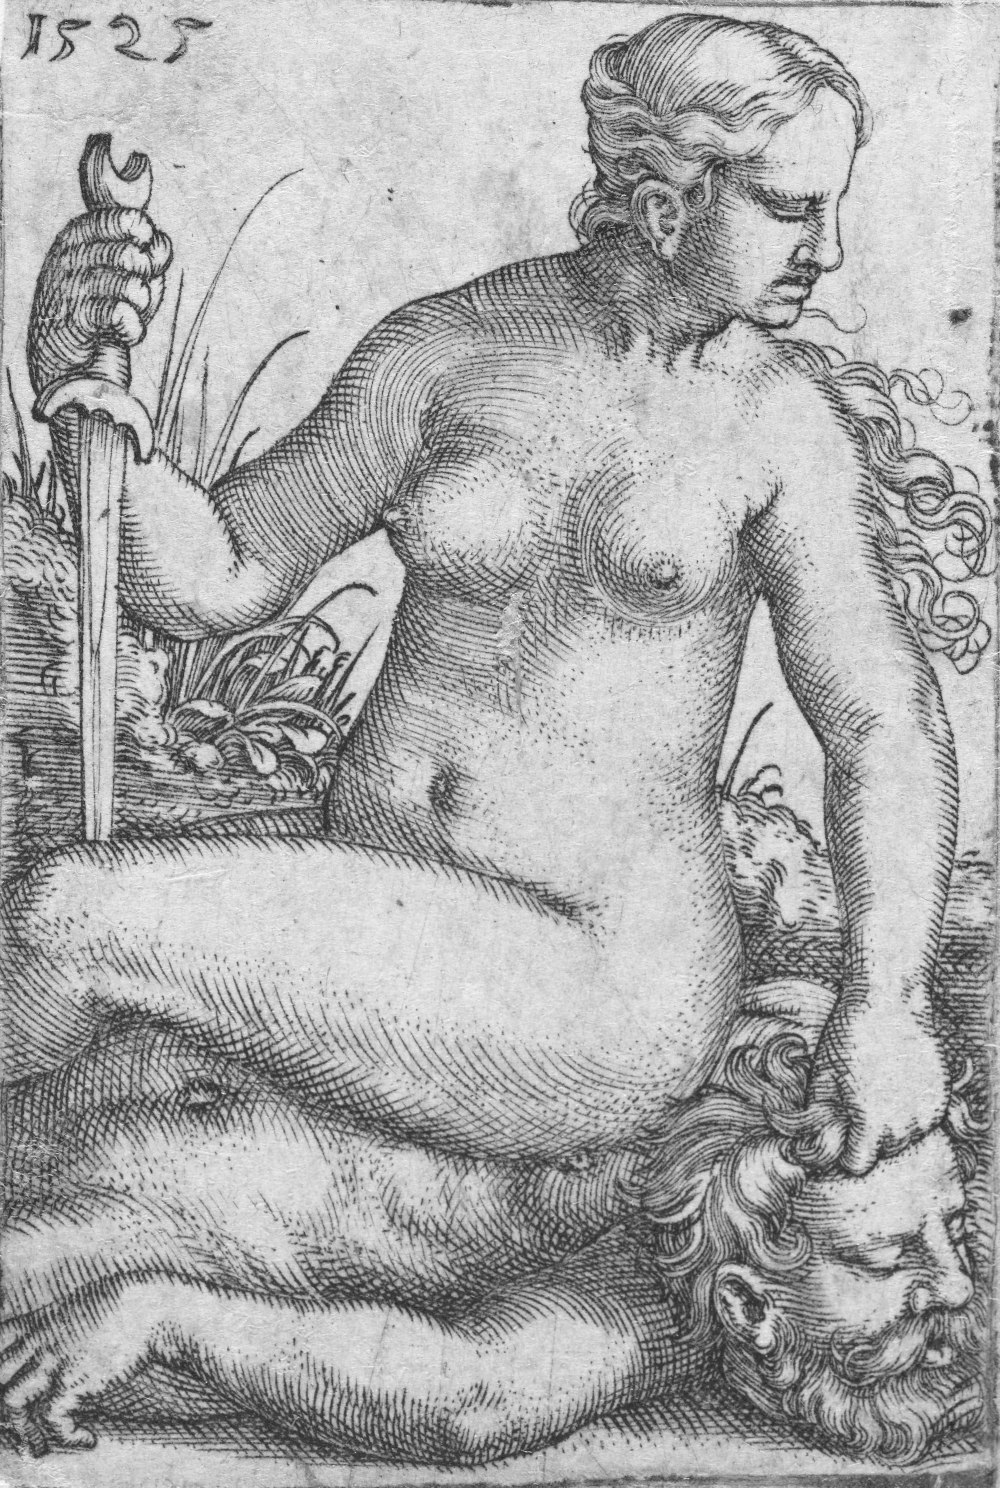
\includegraphics[keepaspectratio,width=0.6\textwidth]{figures/pride-JudithHolofernes-small.jpg}
  \captionart{JudithHolofernes}
  \label{fig:judithholofernes}
\end{figure}

\begin{versewithlinenos}{2}{1}{1}
Nought under heaven so strongly doth allure\\*
The sense of man and all his mind possess,\\*
As beauty's loveliest bait, that doth procure\\*
Great warriors erst their rigour to suppress,\\*
And mighty hands forget their manliness,\\*
Driven with the power of an heart-burning eye,\\*
And lapt in flowers of a golden tress.\\*
That can with melting pleasure mollify\\*
Their harden'd hearts inur'd to cruelty.\\!
\end{versewithlinenos}%
\attrib{\getauthornote{4899} [Book 5 \textlatin{Canto} \rn{VIII.} \theeditor{}]}

\authorfootnote{4900}Clitiphon ingenuously confesseth, that he no sooner came in
Leucippe's presence, but that he did corde tremere, et oculis lascivius
intueri; \authorfootnote{4901}he was wounded at the first sight, his heart panted, and
he could not possibly turn his eyes from her. So doth Calysiris in
Heliodorus, lib. 2. Isis Priest, a reverend old man, complain, who by
chance at Memphis seeing that Thracian Rodophe, might not hold his eyes
off her: \authorfootnote{4902}I will not conceal it, she overcame me with her
presence, and quite assaulted my continency which I had kept unto mine
old age; I resisted a long time my bodily eyes with the eyes of my
understanding; at last I was conquered, and as in a tempest carried
headlong. \authorfootnote{4903} Xenophiles, a philosopher, railed at women downright
for many years together, scorned, hated, scoffed at them; coming at
last into Daphnis a fair maid's company (as he condoles his mishap to
his friend Demaritis), though free before, Intactus nullis ante
cupidinibus, was far in love, and quite overcome upon a sudden. Victus
sum fateor a Daphnide, \etc{}. I confess I am taken,

\li{Sola haec inflexit sensus, animumque labentem
Impulit}---\authorlatintrans{4904.5}\authormarginnote{4904}

I could hold out no longer. Such another mishap, but worse, had
Stratocles the physician, that blear-eyed old man, muco plenus (so
\authorfootnote{4905}Prodromus describes him); he was a severe woman's-hater all his
life, \li{foeda et contumeliosa semper in faeminas profatus}, a bitter
persecutor of the whole sex, \li{humanas aspides et viperas appellabat}, he
forswore them all still, and mocked them wheresoever he came, in such
vile terms, \li{ut matrem et sorores odisses}, that if thou hadst heard him,
thou wouldst have loathed thine own mother and sisters for his word's
sake. Yet this old doting fool was taken at last with that celestial
and divine look of Myrilla, the daughter of Anticles the gardener, that
smirking wench, that he shaved off his bushy beard, painted his face,
\authorfootnote{4906}curled his hair, wore a laurel crown to cover his bald pate, and
for her love besides was ready to run mad. For the very day that he
married he was so furious, ut solis occasum minus expectare posset (a
terrible, a monstrous long day), he could not stay till it was night,
\li{sed omnibus insalutatis in thalamum festinans irrupit}, the meat scarce
out of his mouth, without any leave taking, he would needs go presently
to bed. What young man, therefore, if old men be so intemperate, can
secure himself? Who can say I will not be taken with a beautiful
object? I can, I will contain. No, saith \authorfootnote{4907}Lucian of his mistress,
she is so fair, that if thou dost but see her, she will stupefy thee,
kill thee straight, and, Medusa like, turn thee to a stone; thou canst
not pull thine eyes from her, but, as an adamant doth iron, she will
carry thee bound headlong whither she will herself, infect thee like a
basilisk. It holds both in men and women. Dido was amazed at Aeneas'
presence; \li{Obstupuit primo aspectu Sidonia Dido}; and as he feelingly
verified out of his experience;

\authorfootnote{4908}\li{Quam ego postquam vidi, non ita amavi ut sani solent
Homines, sed eodem pacto ut insani solent}.

\begin{verse}
I lov'd her not as others soberly,\\*
But as a madman rageth, so did I.\\!
\end{verse}

So Museus of Leander, \li{nusquam lumen detorquet ab illa}; and

\begin{verse}
\authormarginnote{4909}Chaucer of Palamon,\\*
He cast his eye upon Emilia,\\*
And therewith he blent and cried ha, ha,\\*
As though he had been stroke unto the hearta.
\end{verse}

If you desire to know more particularly what this beauty is, how it
doth Influere, how it doth fascinate (for, as all hold, love is a
fascination), thus in brief. \authorfootnote{4910}This comeliness or beauty ariseth
from the due proportion of the whole, or from each several part. For an
exact delineation of which, I refer you to poets, historiographers, and
those amorous writers, to Lucian's Images, and Charidemus, Xenophon's
description of Panthea, Petronius Catalectes, Heliodorus Chariclia,
Tacius Leucippe, Longus Sophista's Daphnis and Chloe, Theodorus
Prodromus his Rhodanthes, Aristaenetus and Philostratus Epistles,
Balthazar Castilio, lib. 4. de aulico. Laurentius, cap. 10, de melan.
Aeneas Sylvius his Lucretia, and every poet almost, which have most
accurately described a perfect beauty, an absolute feature, and that
through every member, both in men and women. Each part must concur to
the perfection of it; for as \Seneca{} saith, Ep. 33. lib. 4. Non est
formosa mulier cujus crus laudatur et brachium, sed illa cujus simul
universa facies admirationem singulis partibus dedit; she is no fair
woman, whose arm, thigh, \etc{} are commended, except the face and all the
other parts be correspondent. And the face especially gives a lustre to
the rest: the face is it that commonly denominates a fair or foul: arx
formae facies, the face is beauty's tower; and though the other parts
be deformed, yet a good face carries it (facies non uxor amatur) that
alone is most part respected, principally valued, deliciis suis ferox,
and of itself able to captivate.
\authorfootnote{4911}Urit te Glycerae nitor,
Urit grata protervitas,
Et vultus nimium lubricus aspici.

Glycera's too fair a face was it that set him on fire, too fine to be
beheld. When \authorfootnote{4912}Chaerea saw the singing wench's sweet looks, he was
so taken, that he cried out, O faciem pulchram, deleo omnes dehinc ex
animo mulieres, taedet quotidianarum harum formarum! O fair face, I'll
never love any but her, look on any other hereafter but her; I am weary
of these ordinary beauties, away with them. The more he sees her, the
worse he is,-uritque videndo, as in a burning-glass, the sunbeams are
re-collected to a centre, the rays of love are projected from her eyes.
It was Aeneas's countenance ravished Queen Dido, Os humerosque Deo
similis, he had an angelical face.
\authorfootnote{4913}O sacros vultus Baccho vel Apolline dignos,
Quos vir, quos tuto foemina nulla videt!

---O sacred looks, befitting majesty,
Which never mortal wight could safely see.

Although for the greater part this beauty be most eminent in the face,
yet many times those other members yield a most pleasing grace, and are
alone sufficient to enamour. A high brow like unto the bright heavens,
coeli pulcherrima plaga, Frons ubi vivit honor, frons ubi ludit amor,
white and smooth like the polished alabaster, a pair of cheeks of
vermilion colour, in which love lodgeth; \authorfootnote{4914}Amor qui mollibus genis
puellae pernoctas: a coral lip, suaviorum delubrum, in which Basia
mille patent, basia mille latent, A thousand appear, as many are
concealed; gratiarum sedes gratissima; a sweet-smelling flower, from
which bees may gather honey, \authorfootnote{4915}Mellilegae volucres quid adhuc cava
thyma rosasque, \etc{}.
Omnes ad dominae labra venite meae,
Illa rosas spirat, \etc{}.

A white and round neck, that via lactea, dimple in the chin, black
eyebrows, Cupidinis arcus, sweet breath, white and even teeth, which
some call the salepiece, a fine soft round pap, gives an excellent
grace, \authorfootnote{4916}Quale decus tumidis Pario de marmore mammis! \authorfootnote{4917}and
make a pleasant valley lacteum sinum, between two chalky hills,
Sororiantes papillulas, et ad pruritum frigidos amatores solo aspectu
excitantes. Unde is, \authorfootnote{4918}Forma papillarum quam fuit apta premi!-Again
Urebant oculos durae stantesque mamillae. A flaxen hair; golden hair
was even in great account, for which Virgil commends Dido, Nondum
sustulerat flavum Proserpinina crinem, Et crines nodantur in aurum.
Apollonius (Argonaut. lib. 4. Jasonis flava coma incendit cor Medeae)
will have Jason's golden hair to be the main cause of Medea's dotage on
him. Castor and Pollux were both yellow haired. Paris, Menelaus, and
most amorous young men, have been such in all ages, molles ac suaves,
as Baptista Porta infers, \authorfootnote{4919} Physiog. lib. 2. lovely to behold.
Homer so commends Helen, makes Patroclus and Achilles both yellow
haired: Pulchricoma Venus, and Cupid himself was yellow haired, in
aurum coruscante et crispante capillo, like that neat picture of
Narcissus in Callistratus; for so \authorfootnote{4920}Psyche spied him asleep,
Briseis, Polixena, \etc{} flavicomae omnes,
---and Hero the fair,
Whom young Apollo courted for her hair.

Leland commends Guithera, king Arthur's wife, for a flaxen hair: so
Paulus Aemilius sets out Clodeveus, that lovely king of France.
\authorfootnote{4921}Synesius holds every effeminate fellow or adulterer is fair
haired: and \Apuleius adds that Venus herself, goddess of love, cannot
delight, \authorfootnote{4922}though she come accompanied with the graces, and all
Cupid's train to attend upon her, girt with her own girdle, and smell
of cinnamon and balm, yet if she be bald or badhaired, she cannot
please her Vulcan. Which belike makes our Venetian ladies at this day
to counterfeit yellow hair so much, great women to calamistrate and
curl it up, vibrantes ad gratiam crines, et tot orbibus in captivitatem
flexos, to adorn their heads with spangles, pearls, and made-flowers;
and all courtiers to effect a pleasing grace in this kind. In a word,
\authorfootnote{4923}the hairs are Cupid's nets, to catch all comers, a brushy wood,
in which Cupid builds his nest, and under whose shadow all loves a
thousand several ways sport themselves.

A little soft hand, pretty little mouth, small, fine, long fingers,
Gratiae quae digitis -'tis that which Apollo did admire in
Daphne,-laudat digitosque manusque; a straight and slender body, a
small foot, and well-proportioned leg, hath an excellent lustre,
\authorfootnote{4924}Cui totum incumbit corpus uti fundamento aedes. Clearchus vowed
to his friend Amyander in \authorfootnote{4925}Aristaenetus, that the most attractive
part in his mistress, to make him love and like her first, was her
pretty leg and foot: a soft and white skin, \etc{} have their peculiar
graces, \authorfootnote{4926}Nebula haud est mollior ac hujus cutis est, aedipol
papillam bellulam. Though in men these parts are not so much respected;
a grim Saracen sometimes,-nudus membra Pyracmon, a martial hirsute face
pleaseth best; a black man is a pearl in a fair woman's eye, and is as
acceptable as \authorfootnote{4927}lame Vulcan was to Venus; for he being a sweaty
fuliginous blacksmith, was dearly beloved of her, when fair Apollo,
nimble Mercury were rejected, and the rest of the sweet-faced gods
forsaken. Many women (as Petronius \authorfootnote{4928}observes) sordibus calent (as
many men are more moved with kitchen wenches, and a poor market maid,
than all these illustrious court and city dames) will sooner dote upon
a slave, a servant, a dirt dauber, a brontes, a cook, a player, if they
see his naked legs or arms, thorosaque brachia, \authorfootnote{4929}\etc{}, like that
huntsman Meleager in Philostratus, though he be all in rags, obscene
and dirty, besmeared like a ruddleman, a gipsy, or a chimney-sweeper,
than upon a noble gallant, Nireus, Ephestion, Alcibiades, or those
embroidered courtiers full of silk and gold. \authorfootnote{4930}Justine's wife, a
citizen of Rome, fell in love with Pylades a player, and was ready to
run mad for him, had not Galen himself helped her by chance. Faustina
the empress doted on a fencer.

Not one of a thousand falls in love, but there is some peculiar part or
other which pleaseth most, and inflames him above the rest. \authorfootnote{4931}A
company of young philosophers on a time fell at variance, which part of
a woman was most desirable and pleased best? some said the forehead,
some the teeth, some the eyes, cheeks, lips, neck, chin, \etc{}, the
controversy was referred to Lais of Corinth to decide; but she,
smiling, said, they were a company of fools; for suppose they had her
where they wished, what would they \authorfootnote{4932}first seek? Yet this
notwithstanding I do easily grant, neque quis vestrum negaverit opinor,
all parts are attractive, but especially \authorfootnote{4933}the eyes, \authorfootnote{4934}
---videt igne micantes,
Sideribus similes oculos---

which are love's fowlers; \authorfootnote{4935}aucupium amoris, the shoeing horns, the
hooks of love (as Arandus will) the guides, touchstone, judges, that in
a moment cure mad men, and make sound folks mad, the watchmen of the
body; what do they not? How vex they not? All this is true, and (which
Athaeneus lib. 13. dip. cap. 5. and Tatius hold) they are the chief
seats of love, and James Lernutius \authorfootnote{4936}hath facetely expressed in an
elegant ode of his,
Amorem ocellis flammeolis herae
Vidi insidentem, credite posteri,
Fratresque circum ludibundos
Cum pharetra volitare et arcu, \etc{}.

I saw Love sitting in my mistress' eyes
Sparkling, believe it all posterity,
And his attendants playing round about
With bow and arrows ready for to fly.

Scaliger calls the eyes, \authorfootnote{4937}Cupid's arrows; the tongue, the
lightning of love; the paps, the tents: \authorfootnote{4938}Balthazar Castilio, the
causes, the chariots, the lamps of love,
---aemula lumina stellis,
Lumina quae possent sollicitare deos.

Eyes emulating stars in light,
Enticing gods at the first sight;

Love's orators, Petronius.
O blandos oculos, et o facetos,
Et quadam propria nota loquaces
Illic est Venus, et leves amores,
Atque ipsa in medio sedet voluptas.

O sweet and pretty speaking eyes,
Where Venus, love, and pleasure lies.

Love's torches, touch-box, naphtha and matches, \authorfootnote{4939}Tibullus.
Illius ex oculis quum vult exurere divos,
Accendit geminas lampades acer amor.

Tart Love when he will set the gods on fire,
Lightens the eyes as torches to desire.

Leander, at the first sight of Hero's eyes, was incensed, saith
Musaeus.
Simul in \authorfootnote{4940}oculorum radiis crescebat fax amorum,
Et cor fervebat invecti ignis impetu;
Pulchritudo enim Celebris immaculatae foeminae,
Acutior hominibus est veloci sagitta.
Oculos vero via est, ab oculi ictibus
Vulnus dilabitur, et in praecordia viri manat.

Love's torches 'gan to burn first in her eyes.
And set his heart on fire which never dies:
For the fair beauty of a virgin pure
Is sharper than a dart, and doth inure
A deeper wound, which pierceth to the heart
By the eyes, and causeth such a cruel smart.

\authorfootnote{4941}A modern poet brings in Amnon complaining of Thamar,
---et me fascino
Occidit ille risus et formae lepos,
Ille nitor, illa gratia, et verus decor,
Illae aemulantes purpuram, et \authorfootnote{4942}rosas genae,
Oculique vinctaeque aureo nodo comae.---

It was thy beauty, 'twas thy pleasing smile,
Thy grace and comeliness did me beguile;
Thy rose-like cheeks, and unto purple fair
Thy lovely eyes and golden knotted hair.

\authorfootnote{4943}Philostratus Lemnius cries out on his mistress's basilisk eyes,
ardentes faces, those two burning-glasses, they had so inflamed his
soul, that no water could quench it. What a tyranny (saith he), what a
penetration of bodies is this! thou drawest with violence, and
swallowest me up, as Charybdis doth sailors with thy rocky eyes: he
that falls into this gulf of love, can never get out. Let this be the
corollary then, the strongest beams of beauty are still darted from the
eyes.
\authorfootnote{4944}Nam quis lumina tanta, tanta
Posset luminibus suis tueri,
Non statim trepidansque, palpitansque,
Prae desiderii aestuantis aura? \etc{}.

For who such eyes with his can see,
And not forthwith enamour'd be!

And as men catch dotterels by putting out a leg or an arm, with those
mutual glances of the eyes they first inveigle one another.
\li{Cynthia prima suis miserum me, cepit ocellis}\authorlatintrans{4945.5}\authormarginnote{4945}. Of all eyes (by the
way) black are most amiable, enticing and fairer, which the poet
observes in commending of his mistress. \authorfootnote{4946}Spectandum nigris oculis,
nigroque capillo, which Hesiod admires in his Alemena,
\authorfootnote{4947}Cujus a vertice ac nigricantibus oculis,
Tale quiddam spiral ac ab aurea Venere.

From her black eyes, and from her golden face
As if from Venus came a lovely grace.

and \authorfootnote{4948}Triton in his Milaene-nigra oculos formosa mihi. \authorfootnote{4949}Homer
useth that epithet of ox-eyed, in describing Juno, because a round
black eye is the best, the son of beauty, and farthest from black the
worse: which \authorfootnote{4950}Polydore Virgil taxeth in our nation: Angli ut
plurimum caesiis oculis, we have grey eyes for the most part. Baptisma
Porta, Physiognom. lib. 3. puts grey colour upon children, they be
childish eyes, dull and heavy. Many commend on the other side Spanish
ladies, and those \authorfootnote{4951}Greek dames at this day, for the blackness of
their eyes, as Porta doth his Neapolitan young wives. Suetonius
describes Julius Caesar to have been nigris vegetisque oculis
micantibus, of a black quick sparkling eye: and although Averroes in
his Colliget will have such persons timorous, yet without question they
are most amorous.

Now last of all, I will show you by what means beauty doth fascinate,
bewitch, as some hold, and work upon the soul of a man by the eye. For
certainly I am of the poet's mind, love doth bewitch and strangely
change us.

\authorfootnote{4952}Ludit amor sensus, oculos perstringit, et aufert
Libertatem animi, mira nos fascinat arte.
Credo aliquis daemon subiens praecordia flammam
Concitat, et raptam tollit de cardine mentem.

Love mocks our senses, curbs our liberties,
And doth bewitch us with his art and rings,
I think some devil gets into our entrails,
And kindles coals, and heaves our souls from th'hinges.

Heliodorus lib. 3. proves at large, \authorfootnote{4953}that love is witchcraft, it
gets in at our eyes, pores, nostrils, engenders the same qualities and
affections in us, as were in the party whence it came. The manner of
the fascination, as Ficinus 10. cap. com. in Plat. declares it, is
thus: Mortal men are then especially bewitched, when as by often gazing
one on the other, they direct sight to sight, join eye to eye, and so
drink and suck in love between them; for the beginning of this disease
is the eye. And therefore he that hath a clear eye, though he be
otherwise deformed, by often looking upon him, will make one mad, and
tie him fast to him by the eye. Leonard. Varius, lib. 1. cap. 2. de
fascinat. telleth us, that by this interview, \authorfootnote{4954}the purer spirits
are infected, the one eye pierceth through the other with his rays,
which he sends forth, and many men have those excellent piercing eyes,
that, which Suetonius relates of Augustus, their brightness is such,
they compel their spectators to look off, and can no more endure them
than the sunbeams. \authorfootnote{4955}Barradius, lib. 6. cap. 10. de Harmonia
Evangel. reports as much of our Saviour Christ, and \authorfootnote{4956}Peter Morales
of the Virgin Mary, whom Nicephorus describes likewise to have been
yellow-haired, of a wheat colour, but of a most amiable and piercing
eye. The rays, as some think, sent from the eyes, carry certain
spiritual vapours with them, and so infect the other party, and that in
a moment. I know, they that hold visio fit intra mittendo, will make a
doubt of this; but Ficinus proves it from blear-eyes, \authorfootnote{4957} That by
sight alone, make others blear-eyed; and it is more than manifest, that
the vapour of the corrupt blood doth get in together with the rays, and
so by the contagion the spectators' eyes are infected. Other arguments
there are of a basilisk, that kills afar off by sight, as that Ephesian
did of whom \authorfootnote{4958}Philostratus speaks, of so pernicious an eye, he
poisoned all he looked steadily on: and that other argument, menstruae
faminae, out of Aristotle's Problems, morbosae Capivaccius adds, and
\authorfootnote{4959}Septalius the commentator, that contaminate a looking-glass with
beholding it. \authorfootnote{4960} So the beams that come from the agent's heart, by
the eyes, infect the spirits about the patients, inwardly wound, and
thence the spirits infect the blood. To this effect she complained in
\authorfootnote{4961}\Apuleius, Thou art the cause of my grief, thy eyes piercing
through mine eyes to mine inner parts, have set my bowels on fire, and
therefore pity me that am now ready to die for thy sake. Ficinus
illustrates this with a familiar example of that Marrhusian Phaedrus
and Theban Lycias, \authorfootnote{4962}Lycias he stares on Phaedrus' face, and
Phaedrus fastens the balls of his eyes upon Lycias, and with those
sparkling rays sends out his spirits. The beams of Phaedrus' eyes are
easily mingled with the beams of Lycias, and spirits are joined to
spirits. This vapour begot in Phaedrus' heart, enters into Lycias'
bowels; and that which is a greater wonder, Phaedrus' blood is in
Lycias' heart, and thence come those ordinary love-speeches, my
sweetheart Phaedrus, and mine own self, my dear bowels. And Phaedrus
again to Lycias, O my light, my joy, my soul, my life. Phaedrus follows
Lycias, because his heart would have his spirits, and Lycias follows
Phaedrus, because he loves the seat of his spirits; both follow; but
Lycias the earnester of the two: the river hath more need of the
fountain, than the fountain of the river; as iron is drawn to that
which is touched with a loadstone, but draws not it again; so Lycias
draws Phaedrus. But how comes it to pass then, that the blind man
loves, that never saw? We read in the Lives of the Fathers, a story of
a child that was brought up in the wilderness, from his infancy, by an
old hermit: now come to man's estate, he saw by chance two comely women
wandering in the woods: he asked the old man what creatures they were,
he told him fairies; after a while talking obiter, the hermit demanded
of him, which was the pleasantest sight that ever he saw in his life?
He readily replied, the two \authorfootnote{4963}fairies he spied in the wilderness.
So that, without doubt, there is some secret loadstone in a beautiful
woman, a magnetic power, a natural inbred affection, which moves our
concupiscence, and as he sings,

Methinks I have a mistress yet to come,
And still I seek, I love, I know not whom.

'Tis true indeed of natural and chaste love, but not of this heroical
passion, or rather brutish burning lust of which we treat; we speak of
wandering, wanton, adulterous eyes, which, as \authorfootnote{4964}he saith, lie still
in wait as so many soldiers, and when they spy an innocent spectator
fixed on them, shoot him through, and presently bewitch him: especially
when they shall gaze and gloat, as wanton lovers do one upon another,
and with a pleasant eye-conflict participate each other's souls. Hence
you may perceive how easily and how quickly we may be taken in love;
since at the twinkling of an eye, Phaedrus' spirits may so perniciously
infect Lycias' blood. \authorfootnote{4965}Neither is it any wonder, if we but
consider how many other diseases closely, and as suddenly are caught by
infection, plague, itch, scabs, flux, \etc{}. The spirits taken in, will
not let him rest that hath received them, but egg him on. \li{Idque
petit corpus mens unde est saucia amore}\authorlatintrans{4966.5}\authormarginnote{4966}; and we may manifestly perceive
a strange eduction of spirits, by such as bleed at nose after they be
dead, at the presence of the murderer; but read more of this in
Lemnius, lib. 2. de occult. nat. mir. cap. 7. Valleriola lib. 2.
observ. cap. 7. Valesius controv. Ficinus, Cardan, Libavius de cruentis
cadaveribus, \etc{}.

%SUBSECT. III.-_Artificial allurements of Love, Causes and Provocations to Lust; Gestures, Clothes, Dower, \&c._
\section[Artificial allures of Love]{Artificial allurements of Love, Causes and Provocations to Lust; Gestures, Clothes, Dower, \&c.}

\lettrine{N}{atural} beauty is a stronger loadstone of itself, as you have heard, a
great temptation, and pierceth to the very heart; \li{forma
verecundae, nocuit mihi visa puellae}\authorlatintrans{4967.5}\authormarginnote{4967}; but much more when those
artificial enticements and provocations of gestures, clothes, jewels,
pigments, exornations, shall be annexed unto it; those other
circumstances, opportunity of time and place shall concur, which of
themselves alone were all sufficient, each one in particular to produce
this effect. It is a question much controverted by some wise men, forma
debeat plus arti an naturae? Whether natural or artificial objects be
more powerful? but not decided: for my part I am of opinion, that
though beauty itself be a great motive, and give an excellent lustre in
sordibus, in beggary, as a jewel on a dunghill will shine and cast his
rays, it cannot be suppressed, which Heliodorus feigns of Chariclia,
though she were in beggar's weeds: yet as it is used, artificial is of
more force, and much to be preferred.

\authorfootnote{4968}Sic dentata sibi videtur Aegle,
Emptis ossibus Indicoque cornu;
Sic quae nigrior est cadente moro,
Cerussata sibi placet Lychoris.

So toothless Aegle seems a pretty one,
Set out with new-bought teeth of Indy bone:
So foul Lychoris blacker than berry
Herself admires, now finer than cherry.

John Lerius the Burgundian, cap. 8. hist. navigat. in Brazil. is
altogether on my side. For whereas (saith he) at our coming to Brazil,
we found both men and women naked as they were born, without any
covering, so much as of their privities, and could not be persuaded, by
our Frenchmen that lived a year with them, to wear any, \authorfootnote{4969}Many will
think that our so long commerce with naked women, must needs be a great
provocation to lust; but he concludes otherwise, that their nakedness
did much less entice them to lasciviousness, than our women's clothes.
And I dare boldly affirm (saith he) that those glittering attires,
counterfeit colours, headgears, curled hairs, plaited coats, cloaks,
gowns, costly stomachers, guarded and loose garments, and all those
other accoutrements, wherewith our countrywomen counterfeit a beauty,
and so curiously set out themselves, cause more inconvenience in this
kind, than that barbarian homeliness, although they be no whit inferior
unto them in beauty. I could evince the truth of this by many other
arguments, but I appeal (saith he) to my companions at that present,
which were all of the same mind. His countryman, Montague, in his
essays, is of the same opinion, and so are many others; out of whose
assertions thus much in brief we may conclude, that beauty is more
beholden to art than nature, and stronger provocations proceed from
outward ornaments, than such as nature hath provided. It is true that
those fair sparkling eyes, white neck, coral lips, turgent paps,
rose-coloured cheeks, \etc{}, of themselves are potent enticers; but when
a comely, artificial, well-composed look, pleasing gesture, an affected
carriage shall be added, it must needs be far more forcible than it
was, when those curious needleworks, variety of colours, purest dyes,
jewels, spangles, pendants, lawn, lace, tiffanies, fair and fine linen,
embroideries, calamistrations, ointments, etc. shall be added, they
will make the veriest dowdy otherwise, a goddess, when nature shall be
furthered by art. For it is not the eye of itself that enticeth to
lust, but an adulterous eye, as Peter terms it, 2. \rn{ii.} 14. a wanton, a
rolling, lascivious eye: a wandering eye, which Isaiah taxeth, \rn{iii.} 16.
Christ himself, and the Virgin Mary, had most beautiful eyes, as
amiable eyes as any persons, saith \authorfootnote{4970}Baradius, that ever lived, but
withal so modest, so chaste, that whosoever looked on them was freed
from that passion of burning lust, if we may believe \authorfootnote{4971}Gerson and
\authorfootnote{4972}Bonaventure: there was no such antidote against it, as the Virgin
Mary's face; 'tis not the eye, but carriage of it, as they use it, that
causeth such effects. When Pallas, Juno, Venus, were to win Paris'
favour for the golden apple, as it is elegantly described in that
pleasant interlude of \authorfootnote{4973}\Apuleius, Juno came with majesty upon the
stage, Minerva gravity, but Venus dulce subridens, constitit amaene; et
gratissimae, Graticae deam propitiantes, \etc{} came in smiling with her
gracious graces and exquisite music, as if she had danced, et
nonnunquam saltare solis oculis, and which was the main matter of all,
she danced with her rolling eyes: they were the brokers and harbingers
of her suite. So she makes her brags in a modern poet,
\authormarginnote{4974}Soon could I make my brow to tyrannise,
And force the world do homage to mine eyes.

The eye is a secret orator, the first bawd, Amoris porta, and with
private looks, winking, glances and smiles, as so many dialogues they
make up the match many times, and understand one another's meanings,
before they come to speak a word. \authormarginnote{4975}Euryalus and Lucretia were so
mutually enamoured by the eye, and prepared to give each other
entertainment, before ever they had conference: he asked her good will
with his eyes; she did suffragari, and gave consent with a pleasant
look. That \authormarginnote{4976}Thracian Rodophe was so excellent at this dumb
rhetoric, that if she had but looked upon any one almost (saith
Calisiris) she would have bewitched him, and he could not possibly
escape it. For as \authorfootnote{4977}Salvianus observes, the eyes are the windows of
our souls, by which as so many channels, all dishonest concupiscence
gets into our hearts. They reveal our thoughts, and as they say, frons
animi index, but the eye of the countenance, \authorfootnote{4978}Quid procacibus
intuere ocellis? \etc{}. I may say the same of smiling, gait, nakedness of
parts, plausible gestures, \etc{}. To laugh is the proper passion of a man,
an ordinary thing to smile; but those counterfeit, composed, affected,
artificial and reciprocal, those counter-smiles are the dumb shows and
prognostics of greater matters, which they most part use, to inveigle
and deceive; though many fond lovers again are so frequently mistaken,
and led into a fool's paradise. For if they see but a fair maid laugh,
or show a pleasant countenance, use some gracious words or gestures,
they apply it all to themselves, as done in their favour; sure she
loves them, she is willing, coming, \etc{}.
Stultus quando videt quod pulchra puellula ridet,
Tum fatuus credit se quod amare velit:

When a fool sees a fair maid for to smile,
He thinks she loves him, 'tis but to beguile.

They make an art of it, as the poet telleth us,
\authorfootnote{4979}Quis credat? discunt etiam ridere puellae,
Quaeritur atque illis hac quoque parte decor.

Who can believe? to laugh maids make an art,
And seek a pleasant grace to that same part.

And 'tis as great an enticement as any of the rest,
\authorfootnote{4980}---subrisit molle puella,
Cor tibi rite salit.

She makes thine heart leap with \authorfootnote{4981}a pleasing gentle smile of hers.
\authorfootnote{4982}Dulce ridentem Lalagen amabo,
Dulce loquentem,

I love Lalage as much for smiling, as for discoursing, delectata illa
risit tam blandum, as he said in Petronius of his mistress, being well
pleased, she gave so sweet a smile. It won Ismenias, as he \authorfootnote{4983}
confesseth, Ismene subrisit amatorium, Ismene smiled so lovingly the
second time I saw her, that I could not choose but admire her: and
Galla's sweet smile quite overcame \authorfootnote{4984}Faustus the shepherd, Me
aspiciens moils blande subrisit ocellis. All other gestures of the body
will enforce as much. Daphnis in \authorfootnote{4985}Lucian was a poor tattered wench
when I knew her first, said Corbile, pannosa et Zacera, but now she is
a stately piece indeed, hath her maids to attend her, brave attires,
money in her purse, \etc{}, and will you know how this came to pass? by
setting out herself after the best fashion, by her pleasant carriage,
affability, sweet smiling upon all, \etc{}. Many women dote upon a man for
his compliment only, and good behaviour, they are won in an instant;
too credulous to believe that every light wanton suitor, who sees or
makes love to them, is instantly enamoured, he certainly dotes on,
admires them, will surely marry, when as he means nothing less, 'tis
his ordinary carriage in all such companies. So both delude each other
by such outward shows; and amongst the rest, an upright, a comely
grace, courtesies, gentle salutations, cringes, a mincing gait, a
decent and an affected pace, are most powerful enticers, and which the
prophet Isaiah, a courtier himself, and a great observer, objected to
the daughters of Zion, iii. 16. they minced as they went, and made a
tinkling with their feet. To say the truth, what can they not effect by
such means?

Whilst nature decks them in their best attires
Of youth and beauty which the world admires.

\authormarginnote{4986}\li{Urit-voce, manu, gressu, pectore, fronte, oculis}. When art shall
be annexed to beauty, when wiles and guiles shall concur; for to speak
as it is, love is a kind of legerdemain; mere juggling, a fascination.
When they show their fair hand, fine foot and leg withal, magnum sui
desiderium nobis relinquunt, saith \authorfootnote{4987}Balthazar Castilio, lib. 1.
they set us a longing, and so when they pull up their petticoats, and
outward garments, as usually they do to show their fine stockings, and
those of purest silken dye, gold fringes, laces, embroiderings, (it
shall go hard but when they go to church, or to any other place, all
shall be seen) 'tis but a springe to catch woodcocks; and as
\authorfootnote{4988}\Chrysostom{} telleth them downright, though they say nothing with
their mouths, they speak in their gait, they speak with their eyes,
they speak in the carriage of their bodies. And what shall we say
otherwise of that baring of their necks, shoulders, naked breasts, arms
and wrists, to what end are they but only to tempt men to lust!

\authorfootnote{4989}Nam quid lacteolus sinus, et ipsas
Prae te fers sine linteo papillas?
Hoc est dicere, posce, posce, trado;
Hoc est ad Venerem vocare amantes.

There needs no more, as \authorfootnote{4990}Fredericus Matenesius well observes, but
a crier to go before them so dressed, to bid us look out, a trumpet to
sound, or for defect a sow-gelder to blow,
\authormarginnote{4991}Look out, look out and see
What object this may be
That doth perstringe mine eye;
A gallant lady goes
In rich and gaudy clothes,
But whither away God knows,
---look out, \etc{}, et quae sequuntur,

or to what end and purpose? But to leave all these fantastical
raptures, I'll prosecute my intended theme. Nakedness, as I have said,
is an odious thing of itself, remedium amoris; yet it may be so used,
in part, and at set times, that there can be no such enticement as it
is;
\authorfootnote{4992}Nec mihi cincta Diana placet, nec nuda Cythere,
Illa voluptatis nil habet, haec nimium.

David so espied Bathsheba, the elders Susanna: \authorfootnote{4993}Apelles was
enamoured with Campaspe, when he was to paint her naked. Tiberius in
Suet. cap. 42. supped with Sestius Gallus an old lecher, libidinoso
sene, ea lege ut nudae puellae administrarent; some say as much of
Nero, and Pontus Huter of Carolus Pugnax. Amongst the Babylonians, it
was the custom of some lascivious queans to dance frisking in that
fashion, saith Curtius lib. 5. and Sardus de mor. gent. lib. 1. writes
of others to that effect. The \authorfootnote{4994}Tuscans at some set banquets had
naked women to attend upon them, which Leonicus de Varia hist. lib. 3.
cap. 96. confirms of such other bawdy nations. Nero would have filthy
pictures still hanging in his chamber, which is too commonly used in
our times, and Heliogabalus, etiam coram agentes, ut ad venerem
incitarent: So things may be abused. A servant maid in Aristaenetus
spied her master and mistress through the key-hole \authorfootnote{4995}merrily
disposed; upon the sight she fell in love with her master.
\authorfootnote{4996}Antoninus Caracalla observed his mother-in-law with her breasts
amorously laid open, he was so much moved, that he said, Ah si liceret,
O that I might; which she by chance overhearing, replied as impudently,
\authorfootnote{4997}Quicquid libet licet, thou mayst do what thou wilt: and upon that
temptation he married her: this object was not in cause, not the thing
itself, but that unseemly, indecent carriage of it.
When you have all done, veniunt a veste sagittae the greatest
provocations of lust are from our apparel; God makes, they say, man
shapes, and there is no motive like unto it;
\authorfootnote{4998}Which doth even beauty beautify,
And most bewitch a wretched eye,

a filthy knave, a deformed quean, a crooked carcass, a mawkin, a witch,
a rotten post, a hedgestake may be so set out and tricked up, that it
shall make as fair a show, as much enamour as the rest: many a silly
fellow is so taken. Primum luxuriae, aucupium, one calls it, the first
snare of lust; \authorfootnote{4999}Bossus aucupium animarum, lethalem arundinem, a
fatal reed, the greatest bawd, forte lenocinium, sanguineis lachrymis
deplorandum, saith \authorfootnote{5000}Matenesius, and with tears of blood to be
deplored. Not that comeliness of clothes is therefore to be condemned,
and those usual ornaments: there is a decency and decorum in this as
well as in other things, fit to be used, becoming several persons, and
befitting their estates; he is only fantastical that is not in fashion,
and like an old image in arras hangings, when a manner of attire is
generally received; but when they are so new-fangled, so unstaid, so
prodigious in their attires, beyond their means and fortunes,
unbefitting their age, place, quality, condition, what should we
otherwise think of them? Why do they adorn themselves with so many
colours of herbs, fictitious flowers, curious needleworks, quaint
devices, sweet-smelling odours, with those inestimable riches of
precious stones, pearls, rubies, diamonds, emeralds, \etc{}? Why do they
crown themselves with gold and silver, use coronets and tires of
several fashions, deck themselves with pendants, bracelets, earrings,
chains, girdles, rings, pins, spangles, embroideries, shadows,
rebatoes, versicolour ribands? why do they make such glorious shows
with their scarves, feathers, fans, masks, furs, laces, tiffanies,
ruffs, falls, calls, cuffs, damasks, velvets, tinsels, cloth of gold,
silver, tissue? with colours of heavens, stars, planets: the strength
of metals, stones, odours, flowers, birds, beasts, fishes, and
whatsoever Africa, Asia, America, sea, land, art, and industry of man
can afford? Why do they use and covet such novelty of inventions; such
new-fangled tires, and spend such inestimable sums on them? To what end
are those crisped, false hairs, painted faces, as \authorfootnote{5001}the satirist
observes, such a composed gait, not a step awry? Why are they like so
many Sybarites, or Nero's Poppaea, Ahasuerus' concubines, so costly, so
long a dressing, as Caesar was marshalling his army, or a hawk in
pruning? \li{Dum moliuntur, dum comuntur annus est}\authorlatintrans{5002.5}\authormarginnote{5002}: a \authorfootnote{5003}gardener
takes not so much delight and pains in his garden, a horseman to dress
his horse, scour his armour, a mariner about his ship, a merchant his
shop and shop-book, as they do about their faces, and all those other
parts: such setting up with corks, straightening with whalebones; why
is it, but as a day-net catcheth larks, to make young men stoop unto
them? Philocharus, a gallant in Aristenaetus, advised his friend
Poliaenus to take heed of such enticements, \authorfootnote{5004}for it was the sweet
sound and motion of his mistress's spangles and bracelets, the smell of
her ointments, that captivated him first, Illa fuit mentis prima ruina
meae. Quid sibi vult pixidum turba, saith \authorfootnote{5005}Lucian, to what use are
pins, pots, glasses, ointments, irons, combs, bodkins, setting-sticks?
why bestow they all their patrimonies and husbands' yearly revenues on
such fooleries? \authorfootnote{5006}bina patrimonia singulis auribus; why use they
dragons, wasps, snakes, for chains, enamelled jewels on their necks,
ears? dignum potius foret ferro manus istas religari, atque utinam
monilia vere dracones essent; they had more need some of them be tied
in bedlam with iron chains, have a whip for a fan, and hair-cloths next
to their skins, and instead of wrought smocks, have their cheeks
stigmatised with a hot iron: I say, some of our Jezebels, instead of
painting, if they were well served. But why is all this labour, all
this cost, preparation, riding, running, far-fetched, and dear bought
stuff? \authorfootnote{5007}Because forsooth they would be fair and fine, and where
nature, is defective, supply it by art. \authorfootnote{5008}Sanguine quae vero non
rubet, arte rubet, (\Ovid); and to that purpose they anoint and paint
their faces, to make Helen of Hecuba-parvamque exortamque
puellam-Europen.\authorfootnote{5009}To this intent they crush in their feet and
bodies, hurt and crucify themselves, sometimes in lax-clothes, a
hundred yards I think in a gown, a sleeve; and sometimes again so
close, ut nudos exprimant artus. \authorfootnote{5010}Now long tails and trains, and
then short, up, down, high, low, thick, thin, \etc{}; now little or no
bands, then as big as cart wheels; now loose bodies, then great
farthingales and close girt, \etc{}. Why is all this, but with the whore in
the Proverbs, to intoxicate some or other? oculorum decipulam,\authorfootnote{5011}one
therefore calls it, et indicem libidinis, the trap of lust, and sure
token, as an ivy-bush is to a tavern.

Quod pulchros Glycere sumas de pixide vultus,
Quod tibi compositae nec sine lege comae:

Quod niteat digitis adamas, Beryllus in aure,
Non sum divinus, sed scio quid cupias.


O Glycere, in that you paint so much,
Your hair is so bedeckt in order such.
With rings on fingers, bracelets in your ear,
Although no prophet, tell I can, I fear.

To be admired, to be gazed on, to circumvent some novice; as many times
they do, that instead of a lady he loves a cap and a feather instead of
a maid that should have verum colorem, corpus solidum et succi plenum
(as Chaerea describes his mistress in the \authorfootnote{5012}poet), a painted face,
a ruff-band, fair and fine linen, a coronet, a flower,
(\authorfootnote{5013}Naturaeque putat quod fuit artificis,) a wrought waistcoat he
dotes on, or a pied petticoat, a pure dye instead of a proper woman.
For generally, as with rich-furred conies, their cases are far better
than their bodies, and like the bark of a cinnamon, tree, which is
dearer than the whole bulk, their outward accoutrements are far more
precious than their inward endowments. 'Tis too commonly so.
\authorfootnote{5014}Auferimur cultu, et gemmis, auroque teguntur
Omnia; pars minima est ipsa puella sui.


With gold and jewels all is covered,
And with a strange tire we are won,

(Whilst she's the least part of herself)
And with such baubles quite undone.

Why do they keep in so long together, a whole winter sometimes, and
will not be seen but by torch or candlelight, and come abroad with all
the preparation may be, when they have no business, but only to show
themselves? Spectatum veniunt, veniunt spectentur ut ipsae.
\authorfootnote{5015}For what is beauty if it be not seen,
Or what is't to be seen if not admir'd,
And though admir'd, unless in love desir'd?

why do they go with such counterfeit gait, which \authorfootnote{5016}Philo Judeus
reprehends them for, and use (I say it again) such gestures, apish,
ridiculous, indecent attires, sybaritical tricks, fucos genis,
purpurissam venis, cerussam fronti, leges occulis, \etc{} use those sweet
perfumes, powders and ointments in public; flock to hear sermons so
frequent, is it for devotion? or rather, as \authorfootnote{5017}Basil tells them, to
meet their sweethearts, and see fashions; for, as he saith, commonly
they come so provided to that place, with such curious compliments,
with such gestures and tires, as if they should go to a dancing-school,
a stage-play, or bawdy-house, fitter than a church.
When such a she-priest comes her mass to say,
Twenty to one they all forget to pray.

They make those holy temples, consecrated to godly martyrs and
religious uses, the shops of impudence, dens of whores and thieves, and
little better than brothel houses. When we shall see these things daily
done, their husbands bankrupts, if not cornutos, their wives light
housewives, daughters dishonest; and hear of such dissolute acts, as
daily we do, how should we think otherwise? what is their end, but to
deceive and inveigle young men? As tow takes fire, such enticing
objects produce their effect, how can it be altered? When Venus stood
before Anchises (as \authorfootnote{5018}Homer feigns in one of his hymns) in her
costly robes, he was instantly taken,
Cum ante ipsum staret Jovis filia, videns eam
Anchises, admirabatur formam, et stupendas vestes;
Erat enim induta peplo, igneis radiis spiendidiore;
Habebat quoque torques fulgidos, flexiles haelices,
Tenerum collum ambiebant monilia pulchra,
Aurea, variegata.---

When Venus stood before Anchises first,
He was amaz'd to see her in her tires;
For she had on a hood as red as fire,
And glittering chains, and ivy-twisted spires,
About her tender neck were costly brooches,
And necklaces of gold, enamell'd ouches.

So when Medea came in presence of Jason first, attended by her nymphs
and ladies, as she is described by \authorfootnote{5019}Apollonius,
Cunctas vero ignis instar sequebatur splendor,
Tantum ab aureis fimbriis resplendebat jubar,
Accenditque in oculis dulce desiderium.

A lustre followed them like flaming fire,
And from their golden borders came such beams,
Which in his eyes provok'd a sweet desire.

Such a relation we have in \authorfootnote{5020}Plutarch, when the queens came and
offered themselves to Antony, \authorfootnote{5021}with diverse presents, and enticing
ornaments, Asiatic allurements, with such wonderful joy and festivity,
they did so inveigle the Romans, that no man could contain himself, all
was turned to delight and pleasure. The women transformed themselves to
Bacchus shapes, the men-children to Satyrs and Pans; but Antony himself
was quite besotted with Cleopatra's sweet speeches, philters, beauty,
pleasing tires: for when she sailed along the river Cydnus, with such
incredible pomp in a gilded ship, herself dressed like Venus, her maids
like the Graces, her pages like so many Cupids, Antony was amazed, and
rapt beyond himself. Heliodorus, lib. 1. brings in Dameneta, stepmother
to Cnemon, whom she \authorfootnote{5022}saw in his scarves, rings, robes, and
coronet, quite mad for the love of him. It was Judith's pantofles that
ravished the eyes of Holofernes. And \authorfootnote{5023}Cardan is not ashamed to
confess, that seeing his wife the first time all in white, he did
admire and instantly love her. If these outward ornaments were not of
such force, why doth \authorfootnote{5024}Naomi give Ruth counsel how to please Boaz?
and \authorfootnote{5025}Judith, seeking to captivate Holofernes, washed and anointed
herself with sweet ointments, dressed her hair, and put on costly
attires. The riot in this kind hath been excessive in times past; no
man almost came abroad, but curled and anointed,
\authorfootnote{5026}Et matutino suadans Crispinus amomo.
Quantum vix redolent duo funera.

one spent as much as two funerals at once, and with perfumed hairs,
\authorfootnote{5027}et rosa canos odorati capillos Assyriaque nardo. What strange
thing doth \authorfootnote{5028}Sueton. relate in this matter of Caligula's riot? And
\Pliny{}, lib. 12. \& 13. Read more in Dioscorides, Ulmus, Arnoldus,
Randoletius de fuco et decoratione; for it is now an art, as it was of
old, (so \authorfootnote{5029}\Seneca{} records) officinae, sunt adores coquentium. Women
are bad and men worse, no difference at all between their and our
times; \authorfootnote{5030}good manners (as \Seneca{} complains) are extinct with
wantonness, in tricking up themselves men go beyond women, they wear
harlots' colours, and do not walk, but jet and dance, hic mulier, haec
vir, more like players, butterflies, baboons, apes, antics, than men.
So ridiculous, moreover, we are in our attires, and for cost so
excessive, that as Hierome said of old, Uno filio villarum insunt
pretia, uno lino decies sestertium inseritur; 'tis an ordinary thing to
put a thousand oaks and a hundred oxen into a suit of apparel, to wear
a whole manor on his back. What with shoe-ties, hangers, points, caps
and feathers, scarves, bands, curls, \etc{}, in a short space their whole
patrimonies are consumed. Heliogabalus is taxed by Lampridius, and
admired in his age for wearing jewels in his shoes, a common thing in
our times, not for emperors and princes, but almost for serving men and
tailors; all the flowers, stars, constellations, gold and precious
stones do condescend to set out their shoes. To repress the luxury of
those Roman matrons, there was \authorfootnote{5031}Lex Valeria and Oppia, and a Cato
to contradict; but no laws will serve to repress the pride and
insolency of our days, the prodigious riot in this kind. Lucullus's
wardrobe is put down by our ordinary citizens; and a cobbler's wife in
Venice, a courtesan in Florence, is no whit inferior to a queen, if our
geographers say true: and why is all this? Why do they glory in their
jewels (as \authorfootnote{5032}he saith) or exult and triumph in the beauty of
clothes? why is all this cost? to incite men the sooner to burning
lust. They pretend decency and ornament; but let them take heed, that
while they set out their bodies they do not damn their souls; 'tis
\authorfootnote{5033}Bernard's counsel: shine in jewels, stink in conditions; have
purple robes, and a torn conscience. Let them take heed of Isaiah's
prophecy, that their slippers and attires be not taken from them, sweet
balls, bracelets, earrings, veils, wimples, crisping-pins, glasses,
fine linen, hoods, lawns, and sweet savours, they become not bald,
burned, and stink upon a sudden. And let maids beware, as \authorfootnote{5034}Cyprian
adviseth, that while they wander too loosely abroad, they lose not
their virginities: and like Egyptian temples, seem fair without, but
prove rotten carcases within. How much better were it for them to
follow that good counsel of Tertullian? \authorfootnote{5035}To have their eyes
painted with chastity, the Word of God inserted into their ears,
Christ's yoke tied to the hair, to subject themselves to their
husbands. If they would do so, they should be comely enough, clothe
themselves with the silk of sanctity, damask of devotion, purple of
piety and chastity, and so painted, they shall have God himself to be a
suitor: let whores and queans prank up themselves, \authorfootnote{5036}let them paint
their faces with minion and ceruse, they are but fuels of lust, and
signs of a corrupt soul: if ye be good, honest, virtuous, and religious
matrons, let sobriety, modesty and chastity be your honour, and God
himself your love and desire. Mulier recte olet, ubi nihil olet, then a
woman smells best, when she hath no perfume at all; no crown, chain, or
jewel (Guivarra adds) is such an ornament to a virgin, or virtuous
woman, quam virgini pudor, as chastity is: more credit in a wise man's
eye and judgment they get by their plainness, and seem fairer than they
that are set out with baubles, as a butcher's meat is with pricks,
puffed up, and adorned like so many jays with variety of colours. It is
reported of Cornelia, that virtuous Roman lady, great Scipio's
daughter, Titus Sempronius' wife, and the mother of the Gracchi, that
being by chance in company with a companion, a strange gentlewoman
(some light housewife belike, that was dressed like a May lady, and, as
most of our gentlewomen are, was \authorfootnote{5037}more solicitous of her head-tire
than of her health, that spent her time between a comb and a glass, and
had rather be fair than honest (as Cato said), and have the
commonwealth turned topsy-turvy than her tires marred; and she did
nought but brag of her fine robes and jewels, and provoked the Roman
matron to show hers: Cornelia kept her in talk till her children came
from school, and these, said she, are my jewels, and so deluded and put
off a proud, vain, fantastical, housewife. How much better were it for
our matrons to do as she did, to go civilly and decently,
\authorfootnote{5038}Honestae mulieris instar quae utitur auro pro eo quod est, ad ea
tantum quibus opus est, to use gold as it is gold, and for that use it
serves, and when they need it, than to consume it in riot, beggar their
husbands, prostitute themselves, inveigle others, and peradventure damn
their own souls? How much more would it be for their honour and credit?
Thus doing, as Hierom said of Blesilla, \authorfootnote{5039}Furius did not so triumph
over the Gauls, Papyrius of the Samnites, Scipio of Numantia, as she
did by her temperance; pulla semper veste, \etc{}, they should insult and
domineer over lust, folly, vainglory, all such inordinate, furious and
unruly passions.

But I am over tedious, I confess, and whilst I stand gaping after fine
clothes, there is another great allurement, (in the world's eye at
least) which had like to have stolen out of sight, and that is money,
veniunt a dote sagittae, money makes the match; \authorfootnote{5040}\textgreek{Μονὸν ἄργυρον
βλέπουσιν}: 'tis like sauce to their meat, cum carne condimentum, a good
dowry with a wife. Many men if they do hear but of a great portion, a
rich heir, are more mad than if they had all the beauteous ornaments,
and those good parts art and nature can afford, they \authorfootnote{5041}care not for
honesty, bringing up, birth, beauty, person, but for money.
\authorfootnote{5042}Canes et equos (o Cyrne) quaerimus
Nobiles, et a bona progenie;
Malam vero uxorem, malique patris filiam
Ducere non curat vir bonus,
Modo ei magnam dotem afferat,

Our dogs and horses still from the best breed
We carefully seek, and well may they speed:
But for our wives, so they prove wealthy,
Fair or foul, we care not what they be.

If she be rich, then she is fair, fine, absolute and perfect, then they
burn like fire, they love her dearly, like pig and pie, and are ready
to hang themselves if they may not have her. Nothing so familiar in
these days, as for a young man to marry an old wife, as they say, for a
piece of gold; asinum auro onustum; and though she be an old crone, and
have never a tooth in her head, neither good conditions, nor a good
face, a natural fool, but only rich, she shall have twenty young
gallants to be suitors in an instant. As she said in Suetonius, non me,
sed mea ambiunt, 'tis not for her sake, but for her lands or money; and
an excellent match it were (as he added) if she were away. So on the
other side, many a young lovely maid will cast away herself upon an
old, doting, decrepit dizzard,
\authorfootnote{5043}Bis puer effoeto quamvis balbutiat ore,
Prima legit rarae tam culta roseta puellae,

that is rheumatic and gouty, hath some twenty diseases, perhaps but one
eye, one leg, never a nose, no hair on his head, wit in his brains, nor
honesty, if he have land or \authorfootnote{5044}money, she will have him before all
other suitors, \authorfootnote{5045}Dummodo sit dives barbarus ille placet. If he be
rich, he is the man, a fine man, and a proper man, she will go to
Jacaktres or Tidore with him; Galesimus de monte aureo. Sir Giles
Goosecap, Sir Amorous La-Fool, shall have her. And as Philemasium in
\authorfootnote{5046} Aristaenetus told Emmusus, absque argento omnia vana, hang him
that hath no money, 'tis to no purpose to talk of marriage without
means, \authorfootnote{5047} trouble me not with such motions; let others do as they
will, I'll be sure to have one shall maintain me fine and brave. Most
are of her mind, \authorfootnote{5048} De moribus ultima fiet questio, for his
conditions, she shall inquire after them another time, or when all is
done, the match made, and everybody gone home. \authorfootnote{5049}Lucian's Lycia was
a proper young maid, and had many fine gentlemen to her suitors;
Ethecles, a senator's son, Melissus, a merchant, \etc{}; but she forsook
them all for one Passius, a base, hirsute, bald-pated knave; but why
was it? His father lately died and left him sole heir of his goods and
lands. This is not amongst your dust-worms alone, poor snakes that will
prostitute their souls for money, but with this bait you may catch our
most potent, puissant, and illustrious princes. That proud upstart
domineering Bishop of Ely, in the time of Richard the First, viceroy in
his absence, as \authorfootnote{5050}Nubergensis relates it, to fortify himself, and
maintain his greatness, propinquarum suarum connubiis, plurimos sibi
potentes et nobiles devincire curavit, married his poor kinswomen
(which came forth of Normandy by droves) to the chiefest nobles of the
land, and they were glad to accept of such matches, fair or foul, for
themselves, their sons, nephews, \etc{}. Et quis tam praeclaram aflinitatem
sub spe magnae promotionis non optaret? Who would not have done as much
for money and preferment? as mine author \authorfootnote{5051}adds. Vortiger, King of
Britain, married Rowena the daughter of Hengist the Saxon prince, his
mortal enemy; but wherefore? she had Kent for her dowry. Iagello the
great Duke of Lithuania, 1386, was mightily enamoured on Hedenga,
insomuch that he turned Christian from a Pagan, and was baptised
himself by the name of Uladislaus, and all his subjects for her sake:
but why was it? she was daughter and heir of Poland, and his desire was
to have both kingdoms incorporated into one. Charles the Great was an
earnest suitor to Irene the Empress, but, saith \authorfootnote{5052}Zonarus, ob
regnum, to annex the empire of the East to that of the West. Yet what
is the event of all such matches, that are so made for money, goods, by
deceit, or for burning lust, quos foeda libido conjunxit, what follows?
they are almost mad at first, but 'tis a mere flash; as chaff and straw
soon fired, burn vehemently for a while, yet out in a moment; so are
all such matches made by those allurements of burning lust; where there
is no respect of honesty, parentage, virtue, religion, education, and
the like, they are extinguished in an instant, and instead of love
comes hate; for joy, repentance and desperation itself. Franciscus
Barbarus in his first book de re uxoria, c. 5, hath a story of one
Philip of Padua that fell in love with a common whore, and was now
ready to run mad for her; his father having no more sons let him enjoy
her; \authorfootnote{5053}but after a few days, the young man began to loath, could
not so much as endure the sight of her, and from one madness fell into
another. Such event commonly have all these lovers; and he that so
marries, or for such respects, let them look for no better success than
Menelaus had with Helen, Vulcan with Venus, Theseus with Phaedra, Minos
with Pasiphae, and Claudius with Messalina; shame, sorrow, misery,
melancholy, discontent.

%SUBSECT. IV.-_Importunity and Opportunity of Time, Place, Conference, Discourse, Singing, Dancing, Music, Amorous Tales, Objects, Kissing, Familiarity, Tokens, Presents, Bribes, Promises, Protestations, Tears, &c._
\section[Importunity and Opportunity of Time, Place\ldots{}]{Importunity and Opportunity of Time, Place, Conference, Discourse, Singing, Dancing, Music, Amorous Tales, Objects, Kissing, Familiarity, Tokens, Presents, Bribes, Promises, Protestations, Tears, \&c.}

\lettrine{A}{ll} these allurements hitherto are afar off, and at a distance; I will
come nearer to those other degrees of love, which are conference,
kissing, dalliance, discourse, singing, dancing, amorous tales,
objects, presents, \etc{}, which as so many sirens steal away the hearts
of men and women. For, as Tacitus observes, l. 2, \authorfootnote{5054}It is no
sufficient trial of a maid's affection by her eyes alone, but you must
say something that shall be more available, and use such other forcible
engines; therefore take her by the hand, wring her fingers hard, and
sigh withal; if she accept this in good part, and seem not to be much
averse, then call her mistress, take her about the neck and kiss her,
\etc{}. But this cannot be done except they first get opportunity of
living, or coming together, ingress, egress, and regress; letters and
commendations may do much, outward gestures and actions: but when they
come to live near one another, in the same street, village, or together
in a house, love is kindled on a sudden. Many a serving-man by reason
of this opportunity and importunity inveigles his master's daughter,
many a gallant loves a dowdy, many a gentleman runs upon his wife's
maids; many ladies dote upon their men, as the queen in Ariosto did
upon the dwarf, many matches are so made in haste, and they are
compelled as it were by \authorfootnote{5055}necessity so to love, which had they been
free, come in company of others, seen that variety which many places
afford, or compared them to a third, would never have looked one upon
another. Or had not that opportunity of discourse and familiarity been
offered, they would have loathed and contemned those whom, for want of
better choice and other objects, they are fatally driven on, and by
reason of their hot blood, idle life, full diet, \etc{}, are forced to
dote upon them that come next. And many times those which at the first
sight cannot fancy or affect each other, but are harsh and ready to
disagree, offended with each other's carriage, like Benedict and
Beatrice in the \authorfootnote{5056}comedy, and in whom they find many faults, by
this living together in a house, conference, kissing, colling, and such
like allurements, begin at last to dote insensibly one upon another.
It was the greatest motive that Potiphar's wife had to dote upon
Joseph, and \authorfootnote{5057}Clitiphon upon Leucippe his uncle's daughter, because
the plague being at Bizance, it was his fortune for a time to sojourn
with her, to sit next her at the table, as he tells the tale himself in
Tatius, lib. 2. (which, though it be but a fiction, is grounded upon
good observation, and doth well express the passions of lovers), he had
opportunity to take her by the hand, and after a while to kiss, and
handle her paps, \etc{}, \authorfootnote{5058} which made him almost mad. Ismenias the
orator makes the like confession in Eustathius, lib. 1, when he came
first to Sosthene's house, and sat at table with Cratistes his friend,
Ismene, Sosthene's daughter, waiting on them with her breasts open,
arms half bare, \authorfootnote{5059}Nuda pedem, discincta sinum, spoliata lacertos;
after the Greek fashion in those times,-\authorfootnote{5060} nudos media plus parte
lacertos, as Daphne was when she fled from Phoebus (which moved him
much), was ever ready to give attendance on him, to fill him drink, her
eyes were never off him, rogabundi oculi, those speaking eyes, courting
eyes, enchanting eyes; but she was still smiling on him, and when they
were risen, that she had got a little opportunity, \authorfootnote{5061}she came and
drank to him, and withal trod upon his toes, and would come and go, and
when she could not speak for the company, she would wring his hand, and
blush when she met him: and by this means first she overcame him
(bibens amorem hauriebam simul), she would kiss the cup and drink to
him, and smile, and drink where he drank on that side of the cup, by
which mutual compressions, kissings, wringing of hands, treading of
feet, \etc{}. Ipsam mihi videbar sorbillare virginem, I sipped and sipped
so long, till at length I was drunk in love upon a sudden.
Philocharinus, in \authorfootnote{5062} Aristaenetus, met a fair maid by chance, a
mere stranger to him, he looked back at her, she looked back at him
again, and smiled withal.
\li{Ille dies lethi primus, primusque malorum
Causa fuit.---}\authorlatintrans{5063.5}\authormarginnote{5063}

It was the sole cause of his farther acquaintance, and love that undid
him. \authorfootnote{5064}O nullis tutum credere blanditiis.
This opportunity of time and place, with their circumstances, are so
forcible motives, that it is impossible almost for two young folks
equal in years to live together, and not be in love, especially in
great houses, princes' courts, where they are idle in summo gradu, fare
well, live at ease, and cannot tell otherwise how to spend their time.
\li{Illic Hippolitum pone, Priapus erit}\authormarginnote{5065}. Achilles was sent by his
mother Thetis to the island of Scyros in the Aegean sea (where
Lycomedes then reigned) in his nonage to be brought up; to avoid that
hard destiny of the oracle (he should be slain at the siege of Troy):
and for that cause was nurtured in Genesco, amongst the king's children
in a woman's habit; but see the event: he compressed Deidamia, the
king's fair daughter, and had a fine son, called Pyrrhus by her. Peter
Abelard the philosopher, as he tells the tale himself, being set by
Fulbertus her uncle to teach Heloise his lovely niece, and to that
purpose sojourned in his house, and had committed agnam tenellam
famelico lupo, I use his own words, he soon got her good will, plura
erant oscula quam sententiae and he read more of love than any other
lecture; such pretty feats can opportunity plea; primum domo conjuncti,
inde animis, \etc{}. But when as I say, nox, vinum, et adolescentia, youth,
wine, and night, shall concur, nox amoris et quietis conscia, 'tis a
wonder they be not all plunged over head and ears in love; for youth is
benigna in amorem, et prona materies, a very combustible matter,
naphtha itself, the fuel of love's fire, and most apt to kindle it. If
there be seven servants in an ordinary house, you shall have three
couple in some good liking at least, and amongst idle persons how
should it be otherwise? Living at \authorfootnote{5066}Rome, saith Aretine's Lucretia,
in the flower of my fortunes, rich, fair, young, and so well brought
up, my conversation, age, beauty, fortune, made all the world admire
and love me. Night alone, that one occasion, is enough to set all on
fire, and they are so cunning in great houses, that they make their
best advantage of it: Many a gentlewoman, that is guilty to herself of
her imperfections, paintings, impostures, will not willingly be seen by
day, but as \authorfootnote{5067}Castilio noteth, in the night, Diem ut glis odit,
taedarum lucem super omnia mavult, she hateth the day like a dormouse,
and above all things loves torches and candlelight, and if she must
come abroad in the day, she covets, as \authorfootnote{5068}in a mercer's shop, a very
obfuscate and obscure sight. And good reason she hath for it: Nocte
latent mendae, and many an amorous gull is fetched over by that means.
Gomesius lib. 3. de sale gen. c. 22. gives instance in a Florentine
gentleman, that was so deceived with a wife, she was so radiantly set
out with rings and jewels, lawns, scarves, laces, gold, spangles, and
gaudy devices, that the young man took her to be a goddess (for he
never saw her but by torchlight); but after the wedding solemnities,
when as he viewed her the next morning without her tires, and in a
clear day, she was so deformed, a lean, yellow, shrivelled, \etc{}, such a
beastly creature in his eyes, that he could not endure to look upon
her. Such matches are frequently made in Italy, where they have no
other opportunity to woo but when they go to church, or, as \authorfootnote{5069}in
Turkey, see them at a distance, they must interchange few or no words,
till such time they come to be married, and then as Sardus lib. 1. cap.
3. de morb. gent. and \authorfootnote{5070}Bohemus relate of those old Lacedaemonians,
the bride is brought into the chamber, with her hair girt about her,
the bridegroom comes in and unties the knot, and must not see her at
all by daylight, till such time as he is made a father by her. In those
hotter countries these are ordinary practices at this day; but in our
northern parts, amongst Germans, Danes, French, and Britons, the
continent of Scandia and the rest, we assume more liberty in such
cases; we allow them, as Bohemus saith, to kiss coming and going, et
modo absit lascivia, in cauponem ducere, to talk merrily, sport, play,
sing, and dance so that it be modestly done, go to the alehouse and
tavern together. And 'tis not amiss, though \authorfootnote{5071} \Chrysostom{}, Cyprian,
Hierome, and some other of the fathers speak bitterly against it: but
that is the abuse which is commonly seen at some drunken matches,
dissolute meetings, or great unruly feasts. \authorfootnote{5072}A young,
pickedevanted, trim-bearded fellow, saith Hierome, will come with a
company of compliments, and hold you up by the arm as you go, and
wringing your fingers, will so be enticed, or entice: one drinks to
you, another embraceth, a third kisseth, and all this while the fiddler
plays or sings a lascivious song; a fourth singles you out to dance,
\authorfootnote{5073}one speaks by beck and signs, and that which he dares not say,
signifies by passions; amongst so many and so great provocations of
pleasure, lust conquers the most hard and crabbed minds, and scarce can
a man live honest amongst feastings, and sports, or at such great
meetings. For as he goes on, \authorfootnote{5074}she walks along and with the
ruffling of her clothes, makes men look at her, her shoes creak, her
paps tied up, her waist pulled in to make her look small, she is
straight girded, her hairs hang loose about her ears, her upper garment
sometimes falls, and sometimes tarries to show her naked shoulders, and
as if she would not be seen, she covers that in all haste, which
voluntarily she showed. And not at feasts, plays, pageants, and such
assemblies, \authorfootnote{5075}but as \Chrysostom objects, these tricks are put in
practice at service time in churches, and at the communion itself. If
such dumb shows, signs, and more obscure significations of love can so
move, what shall they do that have full liberty to sing, dance, kiss,
coll, to use all manner of discourse and dalliance! What shall he do
that is beleaguered of all sides?
\authorfootnote{5076}Quem tot, tam roseae petunt puellae,
Quem cultae cupiunt nurus, amorque
Omnis undique et undecunque et usque,
Omnis ambit Amor, Venusque Hymenque.

After whom so many rosy maids inquire,
Whom dainty dames and loving wights desire,
In every place, still, and at all times sue,
Whom gods and gentle goddesses do woo.

How shall he contain? The very tone of some of their voices, a pretty
pleasing speech, an affected tone they use, is able of itself to
captivate a young man; but when a good wit shall concur, art and
eloquence, fascinating speech, pleasant discourse, sweet gestures, the
Sirens themselves cannot so enchant. \authorfootnote{5077}P. Jovius commends his
Italian countrywomen, to have an excellent faculty in this kind, above
all other nations, and amongst them the Florentine ladies: some prefer
Roman and Venetian courtesans, they have such pleasing tongues, and
such \authorfootnote{5078} elegancy of speech, that they are able to overcome a saint,
Pro facie multis vox sua lena fuit. Tanta gratia vocis famam
conciliabat, saith Petronius \authorfootnote{5079}in his fragment of pure impurities,
I mean his Satyricon, tam dulcis sonus permulcebat aera, ut putares
inter auras cantare Syrenum concordiam; she sang so sweetly that she
charmed the air, and thou wouldst have thought thou hadst heard a
concert of Sirens. O good God, when Lais speaks, how sweet it is!
Philocolus exclaims in Aristenaetus, to hear a fair young gentlewoman
play upon the virginals, lute, viol, and sing to it, which as Gellius
observes, lib. 1. cap. 11. are lascivientium delicicae, the chief
delight of lovers, must needs be a great enticement. Parthenis was so
taken. \li{Mi vox ista avida haurit ab aure animam}\authorlatintrans{5080}: O sister
Harpedona (she laments) I am undone, \authorfootnote{5081}how sweetly he sings, I'll
speak a bold word, he is the properest man that ever I saw in my life:
O how sweetly he sings, I die for his sake, O that he would love me
again! If thou didst but hear her sing, saith \authorfootnote{5082}Lucian, thou
wouldst forget father and mother, forsake all thy friends, and follow
her. Helena is highly commended by \authorfootnote{5083}Theocritus the poet for her
sweet voice and music; none could play so well as she, and Daphnis in
the same Edyllion,
Quam tibi os dulce est, et vox amabilis o Daphni,
Jucundius est audire te canentem, quam mel lingere!

How sweet a face hath Daphne, how lovely a voice!
Honey itself is not so pleasant in my choice.

A sweet voice and music are powerful enticers. Those Samian singing
wenches, Aristonica, Onanthe and Agathocleia, regiis diadematibus
insultarunt, insulted over kings themselves, as \authorfootnote{5084}Plutarch
contends. Centum luminibus cinctum caput Argus habebat, Argus had a
hundred eyes, all so charmed by one silly pipe, that he lost his head.
Clitiphon complains in \authorfootnote{5085}Tatius of Leucippe's sweet tunes, he heard
her play by chance upon the lute, and sing a pretty song to it in
commendations of a rose, out of old Anacreon belike;
Rosa honor decusque florum,
Rosa flos odorque divum,
Hominum rosa est voluptas,
Decus illa Gratiarum,
Florente amoris hora,
Rosa suavium Diones, \etc{}.

Rose the fairest of all flowers.
Rose delight of higher powers,
Rose the joy of mortal men,
Rose the pleasure of fine women,
Rose the Graces' ornament,
Rose Dione's sweet content.

To this effect the lovely virgin with a melodious air upon her golden
wired harp or lute, I know not well whether, played and sang, and that
transported him beyond himself, and that ravished his heart. It was
Jason's discourse as much as his beauty, or any other of his good
parts, which delighted Medea so much.
\authorfootnote{5086}---Delectabatur enim
Animus simul forma dulcibusque verbis.

It was Cleopatra's sweet voice and pleasant speech which inveigled
Antony, above the rest of her enticements. Verba ligant hominem, ut
taurorum cornua funes, as bulls' horns are bound with ropes, so are
men's hearts with pleasant words. Her words burn as fire, Eccles. \rn{ix.}
10. Roxalana bewitched Suleiman the Magnificent, and Shore's wife by
this engine overcame Edward the Fourth, \authorfootnote{5087}Omnibus una omnes
surripuit Veneres. The wife of Bath in Chaucer confesseth all this out
of her experience.
%
{\gothfont%
\begin{versewithlinenos}{2}{1}{1}%
Some folk desire us for riches.\\*
Some for shape, some for fairness,\\*
Some for that she can sing or dance.\\*
Some for gentleness, or for dalliance.\\!
\end{versewithlinenos}%
}%
\attrib{[Lines FIXME. \theeditor{}]}

\authorfootnote{5088}Peter Aretine's Lucretia telleth as much and more of herself, I
counterfeited honesty, as if I had been virgo virginissima, more than a
vestal virgin, I looked like a wife, I was so demure and chaste, I did
add such gestures, tunes, speeches, signs and motions upon all
occasions, that my spectators and auditors were stupefied, enchanted,
fastened all to their places, like so many stocks and stones. Many
silly gentlewomen are fetched over in like sort, by a company of gulls
and swaggering companions, that frequently belie noblemen's favours,
rhyming Coribantiasmi, Thrasonean Rhadomantes or Bombomachides, that
have nothing in them but a few player's ends and compliments, vain
braggadocians, impudent intruders, that can discourse at table of
knights and lords' combats, like \authorfootnote{5089}Lucian's Leonitiscus, of other
men's travels, brave adventures, and such common trivial news, ride,
dance, sing old ballad tunes, and wear their clothes in fashion, with a
good grace; a fine sweet gentleman, a proper man, who could not love
him! She will have him though all her friends say no, though she beg
with him. Some again are incensed by reading amorous toys, Amadis de
Gaul, Palmerin de Oliva, the Knight of the Sun, \etc{}, or hearing such
tales of \authorfootnote{5090}lovers, descriptions of their persons, lascivious
discourses, such as Astyanassa, Helen's waiting-woman, by the report of
Suidas, writ of old, de variis concubitus modis, and after her Philenis
and Elephantine; or those light tracts of\authorfootnote{5091}Aristides Milesius
(mentioned by Plutarch) and found by the Persians in Crassus' army
amongst the spoils, Aretine's dialogues, with ditties, love songs, \etc{},
must needs set them on fire, with such like pictures, as those of
Aretine, or wanton objects of what kind soever; no stronger engine than
to hear or read of love toys, fables and discourses (\authorfootnote{5092}one saith)
and many by this means are quite mad. At Abdera in Thrace (Andromeda
one of Euripides' tragedies being played) the spectators were so much
moved with the object, and those pathetical love speeches of Perseus,
amongst the rest, O Cupid, Prince of Gods and men, \etc{} that every man
almost a good while after spake pure iambics, and raved still on
Perseus' speech, O Cupid, Prince of Gods and men. As carmen, boys and
apprentices, when a new song is published with us, go singing that new
tune still in the streets, they continually acted that tragical part of
Perseus, and in every man's mouth was O Cupid, in every street, O
Cupid, in every house almost, O Cupid, Prince of Gods and men,
pronouncing still like stage-players, O Cupid; they were so possessed
all with that rapture, and thought of that pathetical love speech, they
could not a long time after forget, or drive it out of their minds, but
O Cupid, Prince of Gods and men, was ever in their mouths. This belike
made Aristotle, Polit. lib. 7. cap. 18. forbid young men to see
comedies, or to hear amorous tales.
\authorfootnote{5093}Haec igitur juvenes nequam facilesque puellae
Inspiciant---

let not young folks meddle at all with such matters. And this made the
Romans, as \authorfootnote{5094}Vitruvius relates, put Venus' temple in the suburbs,
extra murum, ne adolescentes venereis insuescant, to avoid all
occasions and objects. For what will not such an object do? Ismenias,
as he walked in Sosthene's garden, being now in love, when he saw so
many \authorfootnote{5095}lascivious pictures, Thetis' marriage, and I know not what,
was almost beside himself. And to say truth, with a lascivious object
who is not moved, to see others dally, kiss, dance? And much more when
he shall come to be an actor himself.

To kiss and be kissed, which, amongst other lascivious provocations, is
as a burden in a song, and a most forcible battery, as infectious,
\authorfootnote{5096} Xenophon thinks, as the poison of a spider; a great allurement,
a fire itself, prooemium aut anticoenium, the prologue of burning lust
(as \Apuleius adds), lust itself, \authorfootnote{5097}Venus quinta parte sui nectaris
imbuit, a strong assault, that conquers captains, and those all
commanding forces, (\li{Domasque ferro sed domaris osculo}\authorlatintrans{5098.5}\authormarginnote{5098}).
\authorfootnote{5099}Aretine's Lucretia, when she would in kindness overcome a suitor
of hers, and have her desire of him, took him about the neck, and
kissed him again and again, and to that, which she could not otherwise
effect, she made him so speedily and willingly condescend. And 'tis a
continual assault,-\authorfootnote{5100}hoc non deficit incipitque semper, always
fresh, and ready to \authorfootnote{5101}begin as at first, basium nullo fine
terminatur, sed semper recens est, and hath a fiery touch with it.
\li{---Tenta modo tangere corpus,
Jam tua mellifluo membra calore fluent.}\authorlatintrans{5102.5}\authormarginnote{5102}

Especially when they shall be lasciviously given, as he feelingly said,
\authorfootnote{5103}et me praessulum deosculata Fotis, Catenatis lacertis, \authorfootnote{5104}
Obtorto valgiter labello.
\authorfootnote{5105}Valgiis suaviis,
Dum semiulco suavio
Meam puellam suavior,
Anima tunc aegra et saucia
Concurrit ad labia mihi.

The soul and all is moved; \authorfootnote{5106}Jam pluribus osculis labra
crepitabant, animarum quoque mixturam facientes, inter mutuos complexus
animas anhelantes,
\authorfootnote{5107}Haesimus calentes,
Et transfudimus hinc et hinc labellis
Errantes animas, valete curae.

They breathe out their souls and spirits together with their kisses,
saith \authorfootnote{5108}Balthazar Castilio, change hearts and spirits, and mingle
affections as they do kisses, and it is rather a connection of the mind
than of the body. And although these kisses be delightsome and
pleasant, Ambrosial kisses, \authorfootnote{5109}Suaviolum dulci dulcius Ambrosia,
such as \authorfootnote{5110} Ganymede gave Jupiter, Nectare suavius, sweeter than
\authorfootnote{5111}nectar, balsam, honey, \authorfootnote{5112}Oscula merum amorem stillantia,
love-dropping kisses; for
The gilliflower, the rose is not so sweet,
As sugared kisses be when lovers meet;

Yet they leave an irksome impression, like that of aloes or gall,
\authorfootnote{5113}Ut mi ex Ambrosia, mutatum jam foret illud
Suaviolum tristi tristius helleboro.

At first Ambrose itself was not sweeter,
At last black hellebore was not so bitter.

They are deceitful kisses,
\authorfootnote{5114}Quid me mollibus implicas lacertis?
Quid fallacibus osculis inescas? \etc{}.

Why dost within thine arms me lap,
And with false kisses me entrap.

They are destructive, and the more the worse: \authorfootnote{5115}Et quae me perdunt,
oscula mille dabat, they are the bane of these miserable lovers. There
be honest kisses, I deny not, osculum charitatis, friendly kisses,
modest kisses, vestal-virgin kisses, officious and ceremonial kisses,
\etc{}. Osculi sensus, brachiorum amplexus, kissing and embracing are
proper gifts of Nature to a man; but these are too lascivious kisses,
\li{Implicuitque suos circum meet colla lacertos}\authorlatintrans{5116.5}\authormarginnote{5116}, \etc{} too continuate
and too violent, \authorfootnote{5117}Brachia non hederae, non vincunt oscula conchae;
they cling like ivy, close as an oyster, bill as doves, meretricious
kisses, biting of lips, cum additamento: Tam impresso ore (saith
\authorfootnote{5118}Lucian) ut vix labia detrahant, inter deosculandum mordicantes,
tum et os aperientes quoque et mammas attrectantes, \etc{} such kisses as
she gave to Gyton, innumera oscula dedit non repugnanti puero, cervicem
invadens, innumerable kisses, \etc{}. More than kisses, or too homely
kisses: as those that \authorfootnote{5119}he spake of, Accepturus ab ipsa venere 7,
suavia, \etc{} with such other obscenities that vain lovers use, which are
abominable and pernicious. If, as Peter de Ledesmo cas. cons. holds,
every kiss a man gives his wife after marriage, be mortale peccatum, a
mortal sin, or that of \authorfootnote{5120}Hierome, Adulter est quisquis in uxorem
suam ardentior est amator; or that of Thomas Secund. quaest. 154.
artic. 4. contactus et osculum sit mortale peccatum, or that of Durand.
Rational. lib. 1. cap. 10. abstinere debent conjuges a complexu, toto
tempore quo solennitas nuptiarum interdicitur, what shall become of all
such \authorfootnote{5121}immodest kisses and obscene actions, the forerunners of
brutish lust, if not lust itself! What shall become of them that often
abuse their own wives? But what have I to do with this?
That which I aim at, is to show you the progress of this burning lust;
to epitomise therefore all this which I have hitherto said, with a
familiar example out of that elegant Musaeus, observe but with me those
amorous proceedings of Leander and Hero: they began first to look one
on another with a lascivious look,
Oblique intuens inde nutibus,-
Nutibus mutuis inducens in errorem mentem puellae.
Et illa e contra nutibus mutuis juvenis
Leandri quod amorem non renuit, \etc{}. Inde
Adibat in tenebris tacite quidem stringens
Roseos puellae digitos, ex imo suspirabat
Vehementer---Inde
Virginis autem bene olens collum osculatus.
Tale verbum ait amoris ictus stimulo,
Preces audi et amoris miserere mei,  \etc{}.
Sic fatus recusantis persuasit mentem puellae.


With becks and nods he first began
To try the wench's mind.

With becks and nods and smiles again
An answer he did find.

And in the dark he took her by the hand,
And wrung it hard, and sighed grievously,
And kiss'd her too, and woo'd her as he might,
With pity me, sweetheart, or else I die,
And with such words and gestures as there past,
He won his mistress' favour at the last.

The same proceeding is elegantly described by Apollonius in his
Argonautics, between Jason and Medea, by Eustathius in the ten books of
the loves of Ismenias and Ismene, Achilles Tatius between his Clitophon
and Leucippe, Chaucer's neat poem of Troilus and Cresseide; and in that
notable tale in Petronius of a soldier and a gentlewoman of Ephesus,
that was so famous all over Asia for her chastity, and that mourned for
her husband: the soldier wooed her with such rhetoric as lovers use to
do,-placitone etiam pugnabis amori? \etc{} at last, frangi pertinaciam
passa est, he got her good will, not only to satisfy his lust,
\authorfootnote{5122}but to hang her dead husband's body on the cross (which he
watched instead of the thief's that was newly stolen away), whilst he
wooed her in her cabin. These are tales, you will say, but they have
most significant morals, and do well express those ordinary proceedings
of doting lovers.

Many such allurements there are, nods, jests, winks, smiles,
wrestlings, tokens, favours, symbols, letters, valentines, \etc{}. For
which cause belike, Godfridus lib. 2. de amor. would not have women
learn to write. Many such provocations are used when they come in
presence, \authorfootnote{5123}10 they will and will not,
Malo me Galatea petit lasciva puella,
Et fugit ad salices, et se cupit ante videri.


My mistress with an apple woos me,
And hastily to covert goes

To hide herself, but would be seen
With all her heart before, God knows.

Hero so tripped away from Leander as one displeased,
\authorfootnote{5124}Yet as she went full often look'd behind,
And many poor excuses did she find
To linger by the way,---

but if he chance to overtake her, she is most averse, nice and coy,
Denegat et pugnat, sed vult super omnia vinci.

She seems not won, but won she is at length,
In such wars women use but half their strength.

Sometimes they lie open and are most tractable and coming, apt,
yielding, and willing to embrace, to take a green gown, with that
shepherdess in Theocritus, Edyl. 27. to let their coats, \etc{}, to play
and dally, at such seasons, and to some, as they spy their advantage;
and then coy, close again, so nice, so surly, so demure, you had much
better tame a colt, catch or ride a wild horse, than get her favour, or
win her love, not a look, not a smile, not a kiss for a kingdom.
\authorfootnote{5125}Aretine's Lucretia was an excellent artisan in this kind, as she
tells her own tale, Though I was by nature and art most beautiful and
fair, yet by these tricks I seemed to be far more amiable than I was,
for that which men earnestly seek and cannot attain, draws on their
affection with a most furious desire. I had a suitor loved me dearly
(said she), and the \authorfootnote{5126}more he gave me, the more eagerly he wooed
me, the more I seemed to neglect, to scorn him, and which I commonly
gave others, I would not let him see me, converse with me, no, not have
a kiss. To gull him the more, and fetch him over (for him only I aimed
at) I personated mine own servant to bring in a present from a Spanish
count, whilst he was in my company, as if he had been the count's
servant, which he did excellently well perform: \authorfootnote{5127}Comes de monte
Turco, my lord and master hath sent your ladyship a small present, and
part of his hunting, a piece of venison, a pheasant, a few partridges,
 \etc{} (all which she bought with her own money), commends his love and
service to you, desiring you to accept of it in good part, and he means
very shortly to come and see you. Withal she showed him rings, gloves,
scarves, coronets which others had sent her, when there was no such
matter, but only to circumvent him. \authorfootnote{5128}By these means (as she
concludes) I made the poor gentleman so mad, that he was ready to spend
himself, and venture his dearest blood for my sake. Philinna, in
\authorfootnote{5129}Lucian, practised all this long before, as it shall appear unto
you by her discourse; for when Diphilus her sweetheart came to see her
(as his daily custom was) she frowned upon him, would not vouchsafe him
her company, but kissed Lamprius his co-rival, at the same time
\authorfootnote{5130}before his face: but why was it? To make him (as she telleth her
mother that chid her for it) more jealous; to whet his love, to come
with a greater appetite, and to know that her favour was not so easy to
be had. Many other tricks she used besides this (as she there
confesseth), for she would fall out with, and anger him of set purpose,
pick quarrels upon no occasion, because she would be reconciled to him
again. Amantium irae amoris redintegratio, as the old saying is, the
falling out of lovers is the renewing of love; and according to that of
Aristenaetis, jucundiores amorum post injurias deliciae, love is
increased by injuries, as the sunbeams are more gracious after a cloud.
And surely this aphorism is most true; for as Ampelis informs Crisis in
the said Lucian, \authorfootnote{5131}If a lover be not jealous, angry, waspish, apt
to fall out, sigh and swear, he is no true lover. To kiss and coll,
hang about her neck, protest, swear and wish, are but ordinary
symptoms, incipientis adhuc et crescentis amoris signa; but if he be
jealous, angry, apt to mistake, \etc{}, bene speres licet, sweet sister he
is thine own; yet if you let him alone, humour him, please him, \etc{},
and that he perceive once he hath you sure, without any co-rival, his
love will languish, and he will not care so much for you. Hitherto
(saith she) can I speak out of experience; Demophantus a rich fellow
was a suitor of mine, I seemed to neglect him, and gave better
entertainment to Calliades the painter before his face, principio
abiit, verbis me insectatus, at first he went away all in a chafe,
cursing and swearing, but at last he came submitting himself, vowing
and protesting he loved me most dearly, I should have all he had, and
that he would kill himself for my sake. Therefore I advise thee (dear
sister Crisis) and all maids, not to use your suitors over kindly;
insolentes enim sunt hoc cum sentiunt, 'twill make them proud and
insolent; but now and then reject them, estrange thyself, et si me
audies semel atque iterum exclude, shut him out of doors once or twice,
let him dance attendance; follow my counsel, and by this means
\authorfootnote{5132}you shall make him mad, come off roundly, stand to any
conditions, and do whatsoever you will have him. These are the ordinary
practices; yet in the said Lucian, Melissa methinks had a trick beyond
all this; for when her suitor came coldly on, to stir him up, she writ
one of his co-rival's names and her own in a paper, Melissa amat
Hermotimum, Hermotimus Mellissam, causing it to be stuck upon a post,
for all gazers to behold, and lost it in the way where he used to walk;
which when the silly novice perceived, statim ut legit credidit,
instantly apprehended it was so, came raving to me, \etc{} \authorfootnote{5133}and so
when I was in despair of his love, four months after I recovered him
again. Eugenia drew Timocles for her valentine, and wore his name a
long time after in her bosom: Camaena singled out Pamphilus to dance,
at Myson's wedding (some say), for there she saw him first; Felicianus
overtook Caelia by the highway side, offered his service, thence came
further acquaintance, and thence came love. But who can repeat half
their devices? What Aretine experienced, what conceited Lucian, or
wanton Aristenaetus? They will deny and take, stiffly refuse, and yet
earnestly seek the same, repel to make them come with more eagerness,
fly from if you follow, but if averse, as a shadow they will follow you
again, fugientem sequitur, sequentem fugit; with a regaining retreat, a
gentle reluctancy, a smiling threat, a pretty pleasant peevishness they
will put you off, and have a thousand such several enticements. For as
he saith,

\authorfootnote{5134}Non est forma satis, nec quae vult bella videri,
Debet vulgari more placere suis.

Dicta, sales, lusus, sermones, gratia, risus,
Vincunt naturae candidioris opus.


'Tis not enough though she be fair of hue,
For her to use this vulgar compliment:
But pretty toys and jests, and saws and smiles,
As far beyond what beauty can attempt.

\authorfootnote{5135}For this cause belike Philostratus, in his images, makes diverse
loves, some young, some of one age, some of another, some winged, some
of one sex, some of another, some with torches, some with golden
apples, some with darts, gins, snares, and other engines in their
hands, as Propertius hath prettily painted them out, lib. 2. et 29. and
which some interpret, diverse enticements, or diverse affections of
lovers, which if not alone, yet jointly may batter and overcome the
strongest constitutions.

It is reported of Decius, and Valerianus, those two notorious
persecutors of the church, that when they could enforce a young
Christian by no means (as \authorfootnote{5136}Hierome records) to sacrifice to their
idols, by no torments or promises, they took another course to tempt
him: they put him into a fair garden, and set a young courtesan to
dally with him, \authorfootnote{5137}took him about the neck and kissed him, and that
which is not to be named, manibusque attrectare, \etc{}, and all those
enticements which might be used, that whom torments could not, love
might batter and beleaguer. But such was his constancy, she could not
overcome, and when this last engine would take no place, they left him
to his own ways. At \authorfootnote{5138}Berkley in Gloucestershire, there was in
times past a nunnery (saith Gualterus Mapes, an old historiographer,
that lived 400 years since), of which there was a noble and a fair lady
abbess: Godwin, that subtile Earl of Kent, travelling that way,
(seeking not her but hers) leaves a nephew of his, a proper young
gallant (as if he had been sick) with her, till he came back again, and
gives the young man charge so long to counterfeit, till he had
deflowered the abbess, and as many besides of the nuns as he could, and
leaves him withal rings, jewels, girdles, and such toys to give them
still, when they came to visit him. The young man, willing to undergo
such a business, played his part so well, that in short space he got up
most of their bellies, and when he had done, told his lord how he had
sped: \authorfootnote{5139}his lord made instantly to the court, tells the king how
such a nunnery was become a bawdy-house, procures a visitation, gets
them to be turned out, and begs the lands to his own use. This story I
do therefore repeat, that you may see of what force these enticements
are, if they be opportunely used, and how hard it is even for the most
averse and sanctified souls to resist such allurements. John Major in
the life of John the monk, that lived in the days of Theodosius,
commends the hermit to have been a man of singular continency, and of a
most austere life; but one night by chance the devil came to his cell
in the habit of a young market wench that had lost her way, and desired
for God's sake some lodging with him. \authorfootnote{5140}The old man let her in, and
after some common conference of her mishap, she began to inveigle him
with lascivious talk and jests, to play with his beard, to kiss him,
and do worse, till at last she overcame him. As he went to address
himself to that business, she vanished on a sudden, and the devils in
the air laughed him to scorn. Whether this be a true story, or a tale,
I will not much contend, it serves to illustrate this which I have
said.

Yet were it so, that these of which I have hitherto spoken, and such
like enticing baits, be not sufficient, there be many others, which
will of themselves intend this passion of burning lust, amongst which,
dancing is none of the least; and it is an engine of such force, I may
not omit it. Incitamentum libidinis, Petrarch calls it, the spur of
lust. A \authorfootnote{5141} circle of which the devil himself is the centre.
\authorfootnote{5142}Many women that use it, have come dishonest home, most
indifferent, none better. \authorfootnote{5143} Another terms it the companion of all
filthy delights and enticements, and 'tis not easily told what
inconveniences come by it, what scurrile talk, obscene actions, and
many times such monstrous gestures, such lascivious motions, such
wanton tunes, meretricious kisses, homely embracings.
\authorfootnote{5144}---(ut Gaditana canoro
Incipiat prurire choro, plausuque probatae
Ad terram tremula descendant clune puellae,
Irritamentum Veneris languentis)---

that it will make the spectators mad. When that epitomiser of
\authorfootnote{5145}Trogus had to the full described and set out King Ptolemy's riot
as a chief engine and instrument of his overthrow, he adds, tympanum et
tripudium, fiddling and dancing: the king was not a spectator only, but
a principal actor himself. A thing nevertheless frequently used, and
part of a gentlewoman's bringing up, to sing, dance, and play on the
lute, or some such instrument, before she can say her paternoster, or
ten commandments. 'Tis the next way their parents think to get them
husbands, they are compelled to learn, and by that means,
\authorfootnote{5146}Incoestos amores de tenero meditantur ungue; 'tis a great
allurement as it is often used, and many are undone by it. Thaïs, in
Lucian, inveigled Lamprias in a dance, Herodias so far pleased Herod,
that she made him swear to give her what she would ask, John Baptist's
head in a platter. \authorfootnote{5147}Robert, Duke of Normandy, riding by Falais,
spied Arlette, a fair maid, as she danced on a green, and was so much
enamoured with the object, that she must needs lie with her that
night\authormarginnote{5148}. Owen Tudor won Queen Catherine's affection in. a dance, falling
by chance with his head in her lap. Who cannot parallel these stories
out of his experience? Speusippas a noble gallant in \authorfootnote{5149}that Greek
Aristenaetus, seeing Panareta a fair young gentlewoman dancing by
accident, was so far in love with her, that for a long time after he
could think of nothing but Panareta: he came raving home full of
Panareta: Who would not admire her, who would not love her, that should
but see her dance as I did? O admirable, O divine Panareta! I have seen
old and new Rome, many fair cities, many proper women, but never any
like to Panareta, they are dross, dowdies all to Panareta! O how she
danced, how she tripped, how she turned, with what a grace! happy is
that man that shall enjoy her. O most incomparable, only, Panareta!
When Xenophon, in Symposio, or Banquet, had discoursed of love, and
used all the engines that might be devised, to move Socrates, amongst
the rest, to stir him the more, he shuts up all with a pleasant
interlude or dance of Dionysius and Ariadne. \authorfootnote{5150}First Ariadne
dressed like a bride came in and took her place; by and by Dionysius
entered, dancing to the music. The spectators did all admire the young
man's carriage; and Ariadne herself was so much affected with the
sight, that she could scarce sit. After a while Dionysius beholding
Ariadne, and incensed with love, bowing to her knees, embraced her
first, and kissed her with a grace; she embraced him again, and kissed
him with like affection, \etc{}, as the dance required; but they that
stood by, and saw this, did much applaud and commend them both for it.
And when Dionysius rose up, he raised her up with him, and many pretty
gestures, embraces, kisses, and love compliments passed between them:
which when they saw fair Bacchus and beautiful Ariadne so sweetly and
so unfeignedly kissing each other, so really embracing, they swore they
loved indeed, and were so inflamed with the object, that they began to
rouse up themselves, as if they would have flown. At the last when they
saw them still, so willingly embracing, and now ready to go to the
bride-chamber, they were so ravished, with it, that they that were
unmarried, swore they would forthwith marry, and those that were
married called instantly for their horses, and galloped home to their
wives. What greater motive can there be than this burning lust? what so
violent an oppugner? Not without good cause therefore so many general
councils condemn it, so many fathers abhor it, so many grave men speak
against it; Use not the company of a woman, saith Siracides, 8. 4. that
is a singer, or a dancer; neither hear, lest thou be taken in her
craftiness. In circo non tam cernitur quam discitur libido.

\authorfootnote{5151}Haedus holds, lust in theatres is not seen, but learned. Gregory
Nazianzen that eloquent divine, (\authorfootnote{5152}as he relates the story
himself,) when a noble friend of his solemnly invited him with other
bishops, to his daughter Olympia's wedding, refused to come: \authorfootnote{5153}For
it is absurd to see an old gouty bishop sit amongst dancers; he held it
unfit to be a spectator, much less an actor. Nemo saltat sobrius, Tully
writes, he is not a sober man that danceth; for some such reason
(belike) Domitian forbade the Roman senators to dance, and for that
fact removed many of them from the senate. But these, you will say, are
lascivious and Pagan dances, 'tis the abuse that causeth such
inconvenience, and I do not well therefore to condemn, speak against,
or innocently to accuse the best and pleasantest thing (so \authorfootnote{5154}Lucian
calls it) that belongs to mortal men. You misinterpret, I condemn it
not; I hold it notwithstanding an honest disport, a lawful recreation,
if it be opportune, moderately and soberly used: I am of Plutarch's
mind, \authorfootnote{5155}that which respects pleasure alone, honest recreation, or
bodily exercise, ought not to be rejected and contemned: I subscribe to
\authorfootnote{5156}Lucian, 'tis an elegant thing, which cheereth up the mind,
exerciseth the body, delights the spectators, which teacheth many
comely gestures, equally affecting the ears, eyes, and soul itself.
Sallust discommends singing and dancing in Sempronia, not that she did
sing or dance, but that she did it in excess, 'tis the abuse of it; and
Gregory's refusal doth not simply condemn it, but in some folks. Many
will not allow men and women to dance together, because it is a
provocation to lust: they may as well, with Lycurgus and Mahomet, cut
down all vines, forbid the drinking of wine, for that it makes some men
drunk.
\authorfootnote{5157}Nihil prodest quod non laedere posset idem;
Igne quid utilius?---

I say of this as of all other honest recreations, they are like fire,
good and bad, and I see no such inconvenience, but that they may so
dance, if it be done at due times, and by fit persons: and conclude
with Wolfungus \authorfootnote{5158}Hider, and most of our modern divines: Si decorae,
graves, verecundae, plena luce bonorum virorum et matronarum
honestarum, tempestive fiant, probari possunt, et debent. There is a
time to mourn, a time to dance, Eccles. \rn{iii.} 4. Let them take their
pleasures then, and as \authorfootnote{5159} he said of old, young men and maids
flourishing in their age, fair and lovely to behold, well attired, and
of comely carriage, dancing a Greek galliard, and as their dance
required, kept their time, now turning, now tracing, now apart now
altogether, now a courtesy then a caper, \etc{}, and it was a pleasant
sight to see those pretty knots, and swimming figures. The sun and moon
(some say) dance about the earth, the three upper planets about the sun
as their centre, now stationary, now direct, now retrograde, now in
apogee, then in perigee, now swift then slow, occidental, oriental,
they turn round, jump and trace, \Venus{} and \Mercury{} about the sun with those
thirty-three Maculae or Bourbonian planet, circa Solem saltantes
Cytharedum, saith Fromundus. Four Medicean stars dance about Jupiter,
two Austrian about Saturn, \etc{}, and all (belike) to the music of the
spheres. Our greatest counsellors, and staid senators, at some times
dance, as David before the ark, 2 Sam. \rn{vi.} 14. Miriam, Exod. \rn{xv.} 20.
Judith, \rn{xv.} 13. (though the devil hence perhaps hath brought in those
bawdy bacchanals), and well may they do it. The greatest soldiers, as
\authorfootnote{5160} Quintilianus, \authorfootnote{5161}Aemilius Probus, \authorfootnote{5162}Coelius Rhodiginus,
have proved at large, still use it in Greece, Rome, and the most worthy
senators, cantare, saltare. Lucian, Macrobius, Libanus, Plutarch,
Julius, Pollux, Athenaeus, have written just tracts in commendation of
it. In this our age it is in much request in those countries, as in all
civil commonwealths, as Alexander ab Alexandro, lib. 4. cap. 10. et
lib. 2. cap. 25. hath proved at large, \authorfootnote{5163}amongst the barbarians
themselves none so precious; all the world allows it.
\authorfootnote{5164}Divitias contemno tuas, rex Craese, tuamque
Vendo Asiam, unguentis, flore, mero, choreis.

Plato, in his Commonwealth\authormarginnote{5165}, will have dancing-schools to be
maintained, that young folks might meet, be acquainted, see one
another, and be seen; nay more, he would have them dance naked; and
scoffs at them that laugh at it. But Eusebius praepar. Evangel. lib. 1.
cap. 11. and Theodoret lib. 9. curat. graec. affect. worthily lash him
for it; and well they might: for as one saith, \authorfootnote{5166}the very sight of
naked parts causeth enormous, exceeding concupiscences, and stirs up
both men and women to burning lust. There is a mean in all things: this
is my censure in brief; dancing is a pleasant recreation of body and
mind, if sober and modest (such as our Christian dances are); if
tempestively used, a furious motive to burning lust; if as by Pagans
heretofore, unchastely abused. But I proceed.

If these allurements do not take place, for \authorfootnote{5167}Simierus, that great
master of dalliance, shall not behave himself better, the more
effectually to move others, and satisfy their lust, they will swear and
lie, promise, protest, forge, counterfeit, brag, bribe, flatter and
dissemble of all sides. 'Twas Lucretia's counsel in Aretine, Si vis
amica frui, promitte, finge, jura, perjura, jacta, simula, mentire; and
they put it well in practice, as Apollo to Daphne,
\authorfootnote{5168}---mihi Delphica tellus
Et Claros et Tenedos, patareaque regia servit,
Jupiter est genitor---

Delphos, Claros, and Tenedos serve me,
And Jupiter is known my sire to be.

\authorfootnote{5169}The poorest swains will do as much, \authorfootnote{5170}Mille pecus nivei sunt
et mihi vallibus agni; I have a thousand sheep, good store of cattle,
and they are all at her command,
\authorfootnote{5171}---Tibi nos, tibi nostra supellex,
Ruraque servierint---

house, land, goods, are at her service, as he is himself. Dinomachus, a
senator's son in \authorfootnote{5172}Lucian, in love with a wench inferior to him in
birth and fortunes, the sooner to accomplish his desire, wept unto her,
and swore he loved her with all his heart, and her alone, and that as
soon as ever his father died (a very rich man and almost decrepit) he
would make her his wife. The maid by chance made her mother acquainted
with the business, who being an old fox, well experienced in such
matters, told her daughter, now ready to yield to his desire, that he
meant nothing less, for dost thou think he will ever care for thee,
being a poor wench, \authorfootnote{5173}that may have his choice of all the beauties
in the city, one noble by birth, with so many talents, as young, better
qualified, and fairer than thyself? daughter believe him not: the maid
was abashed, and so the matter broke off. When Jupiter wooed Juno first
(Lilius Giraldus relates it out of an old comment on Theocritus) the
better to effect his suit, he turned himself into a cuckoo, and spying
her one day walking alone, separated from the other goddesses, caused a
tempest suddenly to arise, for fear of which she fled to shelter;
Jupiter to avoid the storm likewise flew into her lap, in virginis
Junonis gremium devolavit, whom Juno for pity covered in her
\authorfootnote{5174}apron. But he turned himself forthwith into his own shape, began
to embrace and offer violence unto her, sed illa matris metu abnuebat,
but she by no means would yield, donec pollicitus connubium obtinuit,
till he vowed and swore to marry her, and then she gave consent. This
fact was done at Thornax hill, which ever after was called Cuckoo hill,
and in perpetual remembrance there was a temple erected to Telia Juno
in the same place. So powerful are fair promises, vows, oaths and
protestations. It is an ordinary thing too in this case to belie their
age, which widows usually do, that mean to marry again, and bachelors
too sometimes,
\authorfootnote{5175}Cujus octavum trepidavit aetas,
cernere lustrum;

to say they are younger than they are. Carmides in the said Lucian
loved Philematium, an old maid of forty-five years; \authorfootnote{5176}she swore to
him she was but thirty-two next December. But to dissemble in this
kind, is familiar of all sides, and often it takes. \li{Fallere
credentem res est operosa puellam}\authormarginnote{5177}, 'tis soon done, no such great
mastery, Egregiam vero laudem, et spolia ampla,-and nothing so frequent
as to belie their estates, to prefer their suits, and to advance
themselves. Many men to fetch over a young woman, widows, or whom they
love, will not stick to crack, forge and feign any thing comes next,
bid his boy fetch his cloak, rapier, gloves, jewels, \etc{} in such a
chest, scarlet-golden-tissue breeches, \etc{} when there is no such
matter; or make any scruple to give out, as he did in Petronius, that
he was master of a ship, kept so many servants, and to personate their
part the better take upon them to be gentlemen of good houses, well
descended and allied, hire apparel at brokers, some scavenger or
prick-louse tailors to attend upon them for the time, swear they have
great possessions, \authorfootnote{5178}bribe, lie, cog, and foist how dearly they
love, how bravely they will maintain her, like any lady, countess,
duchess, or queen; they shall have gowns, tiers, jewels, coaches, and
caroches, choice diet,
The heads of parrots, tongues of nightingales,
The brains of peacocks, and of ostriches,
Their bath shall be the juice of gilliflowers,
Spirit of roses and of violets,
The milk of unicorns, \etc{}.

as old Volpone courted Celia in the \authorfootnote{5179}comedy, when as they are no
such men, not worth a groat, but mere sharkers, to make a fortune, to
get their desire, or else pretend love to spend their idle hours, to be
more welcome, and for better entertainment. The conclusion is, they
mean nothing less,
\authorfootnote{5180}Nil metuunt jurare, nihil promittere curant:
Sed simul accupidae mentis satiata libido est,
Dicta nihil metuere, nihil perjuria curant;

Oaths, vows, promises, are much protested;
But when their mind and lust is satisfied,
Oaths, vows, promises, are quite neglected;

though he solemnly swear by the genius of Caesar, by Venus' shrine,
Hymen's deity, by Jupiter, and all the other gods, give no credit to
his words. For when lovers swear, Venus laughs, Venus haec perjuria
ridet, \authorfootnote{5181}Jupiter himself smiles, and pardons it withal, as grave
\authorfootnote{5182}Plato gives out; of all perjury, that alone for love matters is
forgiven by the gods. If promises, lies, oaths, and protestations will
not avail, they fall to bribes, tokens, gifts, and such like feats.
\authorfootnote{5183}Plurimus auro conciliatur amor: as Jupiter corrupted Danae with a
golden shower, and Liber Ariadne with a lovely crown, (which was
afterwards translated into the heavens, and there for ever shines;)
they will rain chickens, florins, crowns, angels, all manner of coins
and stamps in her lap. And so must he certainly do that will speed,
make many feasts, banquets, invitations, send her some present or other
every foot. Summo studio parentur epulae (saith \authorfootnote{5184}Haedus) et
crebrae fiant largitiones, he must be very bountiful and liberal, seek
and sue, not to her only, but to all her followers, friends, familiars,
fiddlers, panders, parasites, and household servants; he must insinuate
himself, and surely will, to all, of all sorts, messengers, porters,
carriers; no man must be unrewarded, or unrespected. I had a suitor
(saith \authorfootnote{5185}Aretine's Lucretia) that when he came to my house, flung
gold and silver about, as if it had been chaff. Another suitor I had
was a very choleric fellow; but I so handled him, that for all his
fuming, I brought him upon his knees. If there had been an excellent
bit in the market, any novelty, fish, fruit, or fowl, muscatel, or
malmsey, or a cup of neat wine in all the city, it was presented
presently to me; though never so dear, hard to come by, yet I had it:
the poor fellow was so fond at last, that I think if I would I might
have had one of his eyes out of his head. A third suitor was a merchant
of Rome, and his manner of wooing was with \authorfootnote{5186}exquisite music,
costly banquets, poems, \etc{}. I held him off till at length he protested,
promised, and swore pro virginitate regno me donaturum, I should have
all he had, house, goods, and lauds, pro concubitu solo; \authorfootnote{5187}neither
was there ever any conjuror, I think, to charm his spirits that used
such attention, or mighty words, as he did exquisite phrases, or
general of any army so many stratagems to win a city, as he did tricks
and devices to get the love of me. Thus men are active and passive, and
women not far behind them in this kind: \li{Audax ad omnia foemina, quae
vel amat, vel odit}.
%
{\gothfont%
\begin{versewithlinenos}{2}{1}{1}%
For half so boldly there can non\\*
Swear and lye as women can.\\!
\end{versewithlinenos}%
}%
\attrib{\getauthornote{5188} [Lines FIXME. \theeditor{}]}

\authorfootnote{5189}They will crack, counterfeit, and collogue as well as the best,
with handkerchiefs, and wrought nightcaps, purses, posies, and such
toys: as he justly complained,
\authorfootnote{5190}Cur mittis violas? nempe ut violentius uret;
Quid violas violis me violenta tuis? \etc{}.

Why dost thou send me violets, my dear?
To make me burn more violent, I fear,
With violets too violent thou art,
To violate and wound my gentle heart.

When nothing else will serve, the last refuge is their tears. Haec
scripsi (testor amorem) mixta lachrymis et suspiriis, 'twixt tears and
sighs, I write this (I take love to witness), saith \authorfootnote{5191}Chelidonia to
Philonius. Lumina quae modo fulmina, jam flumina lachrymarum, those
burning torches are now turned to floods of tears. Aretine's Lucretia,
when her sweetheart came to town, \authorfootnote{5192}wept in his bosom, that he
might be persuaded those tears were shed for joy of his return.
Quartilla in Petronius, when nought would move, fell a weeping, and as
Balthazar Castilio paints them out, \authorfootnote{5193}To these crocodile's tears
they will add sobs, fiery sighs, and sorrowful countenance, pale
colour, leanness, and if you do but stir abroad, these fiends are ready
to meet you at every turn, with such a sluttish neglected habit,
dejected look, as if they were now ready to die for your sake; and how,
saith he, shall a young novice thus beset, escape? But believe them
not.
\li{---animam ne crede puellis,
Namque est foeminea tutior unda fide.}\authorlatintrans{5194.5}\authormarginnote{5194}

Thou thinkest, peradventure, because of her vows, tears, smiles, and
protestations, she is solely thine, thou hast her heart, hand, and
affection, when as indeed there is no such matter, as the \authorfootnote{5195}Spanish
bawd said, gaudet illa habere unum in lecto, alterum in porta, tertium
qui domi suspiret, she will have one sweetheart in bed, another in the
gate, a third sighing at home, a fourth, \etc{}. Every young man she sees
and likes hath as much interest, and shall as soon enjoy her as
thyself. On the other side, which I have said, men are as false, let
them swear, protest, and lie; \li{Quod vobis dicunt, dixerunt mille
puellis}\authorlatintrans{5196.5}\authormarginnote{5196}. They love some of them those eleven thousand virgins at once,
and make them believe, each particular, he is besotted on her, or love
one till they see another, and then her alone; like Milo's wife in
\Apuleius, lib. 2. Si quem conspexerit speciosae formae invenem,
venustate ejus sumitur, et in eum animum intorquet. 'Tis their common
compliment in that case, they care not what they swear, say or do: One
while they slight them, care not for them, rail downright and scoff at
them, and then again they will run mad, hang themselves, stab and kill,
if they may not enjoy them. Henceforth, therefore,-nulla viro juranti
foemina credat, let not maids believe them. These tricks and
counterfeit passions are more familiar with women, \authorfootnote{5197}finem hic
dolori faciet aut vitae dies, miserere amantis, quoth Phaedra to
Hippolitus. Joessa, in \authorfootnote{5198}Lucian, told Pythias, a young man, to move
him the more, that if he would not have her, she was resolved to make
away herself. There is a Nemesis, and it cannot choose but grieve and
trouble thee, to hear that I have either strangled or drowned myself
for thy sake. Nothing so common to this sex as oaths, vows, and
protestations, and as I have already said, tears, which they have at
command; for they can so weep, that one would think their very hearts
were dissolved within them, and would come out in tears; their eyes are
like rocks, which still drop water, diariae lachrymae et sudoris in
modum lurgeri promptae, saith \authorfootnote{5199} Aristaenetus, they wipe away their
tears like sweat, weep with one eye, laugh with the other; or as
children \authorfootnote{5200}weep and cry, they can both together.
\authorfootnote{5201}Neve puellarum lachrymis moveare memento,
Ut flerent oculos erudiere suos.

Care not for women's tears, I counsel thee,
They teach their eyes as much to weep as see.

And as much pity is to be taken of a woman weeping, as of a goose going
barefoot. When Venus lost her son Cupid, she sent a crier about, to bid
every one that met him take heed.
\authorfootnote{5202}Si fleatam aspicias, ne mox fallare, caveto;
Sin arridebit, magis effuge; et oscula si fors
Ferre volet, fugito; sunt oscula noxia, in ipsis
Suntque venena labris \etc{}.

Take heed of Cupid's tears, if cautious.
And of his smiles and kisses I thee tell,
If that he offer't, for they be noxious,
And very poison in his lips doth dwell.

\authorfootnote{5203}A thousand years, as Castilio conceives, will scarce serve to
reckon up those allurements and guiles, that men and women use to
deceive one another with.

%SUBSECT. V.-_Bawds, Philters, Causes_.
\section{Bawds, Philters, Causes.}

\lettrine{W}{hen} all other engines fail, that they can proceed no farther of
themselves, their last refuge is to fly to bawds, panders, magical
philters, and receipts; rather than fail, to the devil himself.
Flectere si nequeunt superos, Acheronta movebunt. And by those indirect
means many a man is overcome, and precipitated into this malady, if he
take not good heed. For these bawds, first, they are everywhere so
common, and so many, that, as he said of old \authorfootnote{5204}Croton, omnes hic
aut captantur, aut captant, either inveigle or be inveigled, we may say
of most of our cities, there be so many professed, cunning bawds in
them. Besides, bawdry is become an art, or a liberal science, as Lucian
calls it; and there be such tricks and subtleties, so many nurses, old
women, panders, letter carriers, beggars, physicians, friars,
confessors, employed about it, that nullus tradere stilus sufficiat,
one saith,
\authorfootnote{5205}---trecentis versibus
Suas impuritias traloqui nemo potest.

Such occult notes, stenography, polygraphy, Nuntius animatus, or
magnetical telling of their minds, which \authorfootnote{5206}Cabeus the Jesuit, by
the way, counts fabulous and false; cunning conveyances in this kind,
that neither Juno's jealousy, nor Danae's custody, nor Argo's vigilancy
can keep them safe. 'Tis the last and common refuge to use an
assistant, such as that Catanean Philippa was to Joan Queen of Naples,
a \authorfootnote{5207}bawd's help, an old woman in the business, as \authorfootnote{5208}Myrrha did
when she doted on Cyniras, and could not compass her desire, the old
jade her nurse was ready at a pinch, dic inquit, opemque me sine ferre
tibi-et in hac mea (pone timorem) Sedulitas erit apta libi, fear it
not, if it be possible to be done, I will effect it: non est mulieri
mulier insuperabilis, \authorfootnote{5209}Caelestina said, let him or her be never so
honest, watched and reserved, 'tis hard but one of these old women will
get access: and scarce shall you find, as \authorfootnote{5210}\Austin{} observes, in a
nunnery a maid alone, if she cannot have egress, before her window you
shall have an old woman, or some prating gossip, tell her some tales of
this clerk, and that monk, describing or commending some young
gentleman or other unto her. As I was walking in the street (saith a
good fellow in Petronius) to see the town served one evening, \authorfootnote{5211}I
spied an old woman in a corner selling of cabbages and roots (as our
hucksters do plums, apples, and such like fruits); mother (quoth he)
can you tell where I can dwell? she, being well pleased with my foolish
urbanity, replied, and why, sir, should I not tell? With that she rose
up and went before me. I took her for a wise woman, and by-and-by she
led me into a by-lane, and told me there I should dwell. I replied
again, I knew not the house; but I perceived, on a sudden, by the naked
queans, that I was now come into a bawdy-house, and then too late I
began to curse the treachery of this old jade. Such tricks you shall
have in many places, and amongst the rest it is ordinary in Venice, and
in the island of Zante, for a man to be bawd to his own wife. No sooner
shall you land or come on shore, but, as the Comical Poet hath it,
\authorfootnote{5212}Morem hunc meretrices habent,
Ad portum mittunt servulos, ancillulas,
Si qua peregrina navis in portum aderit,
Rogant cujatis sit, quod ei nomen siet,
Post illae extemplo sese adplicent.

These white devils have their panders, bawds, and factors in every
place to seek about, and bring in customers, to tempt and waylay
novices, and silly travellers. And when they have them once within
their clutches, as Aegidius Mascrius in his comment upon Valerius
Flaccus describes them, \authorfootnote{5213}with promises and pleasant discourse,
with gifts, tokens, and taking their opportunities, they lay nets which
Lucretia cannot avoid, and baits that Hippolitus himself would swallow;
they make such strong assaults and batteries, that the goddess of
virginity cannot withstand them: give gifts and bribes to move
Penelope, and with threats able to terrify Susanna. How many
Proserpinas, with those catchpoles, doth Pluto take? These are the
sleepy rods with which their souls touched descend to hell; this the
glue or lime with which the wings of the mind once taken cannot fly
away; the devil's ministers to allure, entice, \etc{}. Many young men and
maids, without all question, are inveigled by these Eumenides and their
associates. But these are trivial and well known. The most sly,
dangerous, and cunning bawds, are your knavish physicians, empirics,
mass-priests, monks, Jesuits\authormarginnote{5214}, and friars. Though it be against
Hippocrates' oath, some of them will give a dram, promise to restore
maidenheads, and do it without danger, make an abortion if need be,
keep down their paps, hinder conception, procure lust, make them able
with Satyrions, and now and then step in themselves. No monastery so
close, house so private, or prison so well kept, but these honest men
are admitted to censure and ask questions, to feel their pulse beat at
their bedside, and all under pretence of giving physic. Now as for
monks, confessors, and friars, as he said,
%
\begin{latin}
\begin{verse}
Non audet Stygius Pluto tentare quod audet\\*
Effrenis monachus, plenaque fraudis anus;
\end{verse}
\end{latin}
\translationrule
\begin{verse}
That Stygian Pluto dares not tempt or do,\\*
What an old hag or monk will undergo;
\end{verse}
\attrib{\getauthornote{5215}}

either for himself to satisfy his own lust; for another, if he be hired
thereto, or both at once, having such excellent means. For under colour
of visitation, auricular confession, comfort and penance, they have
free egress and regress, and corrupt, God knows, how many. They can
such trades, some of them, practise physic, use exorcisms, \etc{}.
%
{\gothfont%
\begin{versewithlinenos}{2}{1}{1}%
That whereas was wont to walk and Elf,\\*
There now walks the Limiter himself,\\*
In every bush and under every tree,\\*
There needs no other Incubus but he.\\!
\end{versewithlinenos}%
}%
\attrib{\getauthornote{5216} [Lines FIXME. \theeditor]}

\authorfootnote{5217}In the mountains between Dauphine and Savoy, the friars persuaded
the good wives to counterfeit themselves possessed, that their husbands
might give them free access, and were so familiar in those days with
some of them, that, as one\authorfootnote{5218}observes, wenches could not sleep in
their beds for necromantic friars: and the good abbess in Boccaccio may
in some sort witness, that rising betimes, mistook and put on the
friar's breeches instead of her veil or hat. You have heard the story,
I presume, of \authorfootnote{5219} Paulina, a chaste matron in Aegesippus, whom one
of Isis's priests did prostitute to Mundus, a young knight, and made
her believe it was their god Anubis. Many such pranks are played by our
Jesuits, sometimes in their own habits, sometimes in others, like
soldiers, courtiers, citizens, scholars, gallants, and women
themselves. Proteus-like, in all forms and disguises, that go abroad in
the night, to inescate and beguile young women, or to have their
pleasure of other men's wives; and, if we may believe \authorfootnote{5220} some
relations, they have wardrobes of several suits in the colleges for
that purpose. Howsoever in public they pretend much zeal, seem to be
very holy men, and bitterly preach against adultery, fornication, there
are no verier bawds or whoremasters in a country; \authorfootnote{5221}whose soul they
should gain to God, they sacrifice to the devil. But I spare these men
for the present.

The last battering engines are philters, amulets, spells, charms,
images, and such unlawful means: if they cannot prevail of themselves
by the help of bawds, panders, and their adherents, they will fly for
succour to the devil himself. I know there be those that deny the devil
can do any such thing (Crato epist. 2. lib. med.), and many divines,
there is no other fascination than that which comes by the eyes, of
which I have formerly spoken, and if you desire to be better informed,
read Camerarius, oper subcis. cent. 2. c. 5. It was given out of old,
that a Thessalian wench had bewitched King Philip to dote upon her, and
by philters enforced his love; but when Olympia, the Queen, saw the
maid of an excellent beauty, well brought up, and qualified-these,
quoth she, were the philters which inveigled King Philip; those the
true charms, as Henry to Rosamond,
\authorfootnote{5222}One accent from thy lips the blood more warms,
Than all their philters, exorcisms, and charms.

With this alone Lucretia brags \authorfootnote{5223}in Aretine, she could do more than
all philosophers, astrologers, alchemists, necromancers, witches, and
the rest of the crew. As for herbs and philters, I could never skill of
them, The sole philter that ever I used was kissing and embracing, by
which alone I made men rave like beasts stupefied, and compelled them
to worship me like an idol. In our times it is a common thing, saith
Erastus, in his book de Lamiis, for witches to take upon them the
making of these philters, \authorfootnote{5224}to force men and women to love and hate
whom they will, to cause tempests, diseases, \etc{}, by charms, spells,
characters, knots.-\authorfootnote{5225}hic Thessala vendit Philtra. St. Hierome
proves that they can do it (as in Hilarius' life, epist. lib. 3); he
hath a story of a young man, that with a philter made a maid mad for
the love of him, which maid was after cured by Hilarion. Such instances
I find in John Nider, Formicar. lib. 5. cap. 5. Plutarch records of
Lucullus that he died of a philter; and that Cleopatra used philters to
inveigle Antony, amongst other allurements. Eusebius reports as much of
Lucretia the poet. Panormitan, lib. 4. de gest. Aphonsi, hath a story
of one Stephan, a Neapolitan knight, that by a philter was forced to
run mad for love. But of all others, that which \authorfootnote{5226}Petrarch, epist.
famil. lib. 1. ep. 5, relates of Charles the Great (Charlemagne) is
most memorable. He foolishly doted upon a woman of mean favour and
condition, many years together, wholly delighting in her company, to
the great grief and indignation of his friends and followers. When she
was dead, he did embrace her corpse, as Apollo did the bay-tree for his
Daphne, and caused her coffin (richly embalmed and decked with jewels)
to be carried about with him, over which he still lamented. At last a
venerable bishop, that followed his court, prayed earnestly to God
(commiserating his lord and master's case) to know the true cause of
this mad passion, and whence it proceeded; it was revealed to him, in
fine, that the cause of the emperor's mad love lay under the dead
woman's tongue. The bishop went hastily to the carcass, and took a
small ring thence; upon the removal the emperor abhorred the corpse,
and, instead \authorfootnote{5227}of it, fell as furiously in love with the bishop, he
would not suffer him to be out of his presence; which when the bishop
perceived, he flung the ring into the midst of a great lake, where the
king then was. From that hour the emperor neglected all his other
houses, dwelt at \authorfootnote{5228}Ache, built a fair house in the midst of the
marsh, to his infinite expense, and a \authorfootnote{5229}temple by it, where after
he was buried, and in which city all his posterity ever since use to be
crowned. Marcus the heretic is accused by Irenaeus, to have inveigled a
young maid by this means; and some writers speak hardly of the Lady
Katharine Cobham, that by the same art she circumvented Humphrey Duke
of Gloucester to be her husband. Sycinius Aemilianus summoned
\authorfootnote{5230}\Apuleius to come before Cneius Maximus, proconsul of Africa, that
he being a poor fellow, had bewitched by philters Pudentilla, an
ancient rich matron, to love him, and, being worth so many thousand
sesterces, to be his wife. Agrippa, lib. 1. cap. 48. occult. philos.
attributes much in this kind to philters, amulets, images: and Salmutz
com. in Pancirol. Tit. 10. de Horol. Leo Afer, lib. 3, saith, 'tis an
ordinary practice at Fez in Africa, Praestigiatores ibi plures, qui
cogunt amores et concubitus: as skilful all out as that hyperborean
magician, of whom Cleodemus, in \authorfootnote{5231} Lucian, tells so many fine feats
performed in this kind. But Erastus, Wierus, and others are against it;
they grant indeed such things may be done, but (as Wierus discourseth,
lib. 3. de Lamiis. cap. 37.) not by charms, incantations, philters, but
the devil himself; lib. 5. cap. 2. he contends as much; so doth
Freitagius, noc. med. cap. 74. Andreas Cisalpinus, cap. 5; and so much
Sigismundus Scheretzius, cap. 9. de hirco nocturno, proves at large.

\authorfootnote{5232}Unchaste women by the help of these witches, the devil's kitchen
maids, have their loves brought to them in the night, and carried back
again by a phantasm flying in the air in the likeness of a goat. I have
heard (saith he) diverse confess, that they have been so carried on a
goat's back to their sweethearts, many miles in a night. Others are of
opinion that these feats, which most suppose to be done by charms and
philters, are merely effected by natural causes, as by man's blood
chemically prepared, which much avails, saith Ernestus Burgravius, in
Lucerna vitae et mortis Indice, ad amorem conciliandum et odium, (so
huntsmen make their dogs love them, and farmers their pullen,) 'tis an
excellent philter, as he holds, sed vulgo prodere grande nefas, but not
fit to be made common: and so be Mala insana, mandrake roots, mandrake
\authorfootnote{5233}apples, precious stones, dead men's clothes, candles, mala
Bacchica, panis porcinus, Hyppomanes, a certain hair in a \authormarginnote{5234}wolf's
tail, \etc{}, of which Rhasis, Dioscorides, Porta, Wecker, Rubeus,
Mizaldus, Albertus, treat: a swallow's heart, dust of a dove's heart,
multum valent linguae viperarum, cerebella asinorum, tela equina,
palliola quibus infantes obvoluti nascuntur, funis strangulati hominis,
lapis de nido Aquilae, \etc{}. See more in Sckenkius observat. medicinal,
lib. 4. \etc{}, which are as forcible and of as much virtue as that
fountain Salmacis in \authorfootnote{5235} Vitruvius, \Ovid, Strabo, that made all such
mad for love that drank of it, or that hot bath at \authorfootnote{5236}Aix in
Germany, wherein Cupid once dipped his arrows, which ever since hath a
peculiar virtue to make them lovers all that wash in it. But hear the
poet's own description of it,

\authorfootnote{5237}Unde hic fervor aquis terra erumpentibus uda?
Tela olim hic ludens ignea tinxit amor;

Et gaudens stridore novo, fervete perennes
Inquit, et haec pharetrae sint monumenta meae.

Ex illo fervet, rarusque hic mergitur hospes,
Cui non titillet pectora blandus amor.

These above-named remedies have happily as much power as that bath of
Aix, or Venus' enchanted girdle, in which, saith Natales Comes, Love
toys and dalliance, pleasantness, sweetness, persuasions, subtleties,
gentle speeches, and all witchcraft to enforce love, was contained.
Read more of these in Agrippa de occult. Philos. lib. 1. cap. 50. et
45. Malleus malefic. part. 1. quaest. 7. Delrio tom. 2. quest. 3. lib.
3. Wierus, Pomponatis, cap. 8. de incantat. Ficinus, lib. 13. Theol.
Plat. Calcagninus, \etc{}.

%MEMB. III.

\section[Symptoms or signs of Love Melancholy]{Symptoms or signs of Love Melancholy, in Body, Mind, good, bad, \&c.}

\lettrine{S}{ymptoms} are either of body or mind; of body, paleness, leanness,
dryness, \etc{}. \authorfootnote{5238}Pallidus omnis amans, color hic est aptus amanti, as
the poet describes lovers: fecit amor maciem, love causeth leanness.
\authorfootnote{5239} Avicenna de Ilishi, c. 33. makes hollow eyes, dryness, symptoms
of this disease, to go smiling to themselves, or acting as if they saw
or heard some delectable object. Valleriola, lib. 3. observat. cap. 7.
Laurentius, cap. 10. Aelianus Montaltus de Her. amore. Langius, epist.
24. lib. 1. epist. med. deliver as much, corpus exangue pallet, corpus
gracile, oculi cavi, lean, pale,-ut nudis qui pressit calcibus anguem,
as one who trod with naked foot upon a snake, hollow-eyed, their eyes
are hidden in their heads,-\authorfootnote{5240}Tenerque nitidi corposis cecidit
decor, they pine away, and look ill with waking, cares, sighs.
Et qui tenebant signa Phoebeae facis
Oculi, nihil gentile nec patrium micant.

And eyes that once rivalled the locks of Phoebus, lose the patrial and
paternal lustre. With groans, griefs, sadness, dullness,
\authorfootnote{5241}---Nulla jam Cereris subi
Cura aut salutis---

want of appetite, \etc{}. A reason of all this, \authorfootnote{5242}Jason Pratensis
gives, because of the distraction of the spirits the liver doth not
perform his part, nor turns the aliment into blood as it ought, and for
that cause the members are weak for want of sustenance, they are lean
and pine, as the herbs of my garden do this month of May, for want of
rain. The green sickness therefore often happeneth to young women, a
cachexia or an evil habit to men, besides their ordinary sighs,
complaints, and lamentations, which are too frequent. As drops from a
still,-ut occluso stillat ab igne liquor, doth Cupid's fire provoke
tears from a true lover's eyes,
\authorfootnote{5243}The mighty Mars did oft for Venus shriek,
Privily moistening his horrid cheek
With womanish tears,---

\authorfootnote{5244}---ignis distillat in undas,
Testis erit largus qui rigat ora liquor,

with many such like passions. When Chariclia was enamoured of
Theagines, as \authorfootnote{5245}Heliodorus sets her out, she was half distracted,
and spake she knew not what, sighed to herself, lay much awake, and was
lean upon a sudden: and when she was besotted on her son-in-law,
\authorfootnote{5246}pallor deformis, marcentes oculi, \etc{}, she had ugly paleness,
hollow eyes, restless thoughts, short wind, \etc{}. Euryalus, in an epistle
sent to Lucretia, his mistress, complains amongst other grievances, tu
mihi et somni et cibi usum abstulisti, thou hast taken my stomach and
my sleep from me. So he describes it aright:
%
{\gothfont%
\begin{versewithlinenos}{2}{1361}{1362}%
His sleep, his meat, his drink, in him bereft,\\*
That lean he waxeth, and dry as a shaft,\\*
His eyes hollow and grisly to behold,\\*
His hew pale and ashen to unfold,\\*
And solitary he was ever alone,\\*
And waking all the night making moan.\\!
\end{versewithlinenos}%
}%
\attrib{\getauthornote{5247}}

Theocritus Edyl. 2. makes a fair maid of Delphos, in love with a young
man of Minda, confess as much,
Ut vidi ut insanii, ut animus mihi male affectiis est,
Miserae mihi forma tabescebat, neque amplius pompam
Ullum curabam, aut quando domum redieram
Novi, sed me ardens quidam morbus consumebat,
Decubui in lecto dies decem, et noctes decem,
Defluebant capite capilli, ipsaque sola reliqua
Ossa et cutis---

No sooner seen I had, but mad I was.
My beauty fail'd, and I no more did care
For any pomp, I knew not where I was,
But sick I was, and evil I did fare;
I lay upon my bed ten days and nights,
A skeleton I was in all men's sights.

All these passions are well expressed by \authorfootnote{5248}that heroical poet in
the person of Dido:
At non infelix animi Phaenissa, nec unquam
Solvitur in somnos, oculisque ac pectore amores
Accipit; ingeminant curae, rursusque resurgens
Saevit amor, \etc{}.---

Unhappy Dido could not sleep at all,
But lies awake, and takes no rest:
And up she gets again, whilst care and grief,
And raging love torment her breast.

Accius Sanazarius Egloga 2. de Galatea, in the same manner feigns his
Lychoris \authorfootnote{5249}tormenting herself for want of sleep, sighing, sobbing,
and lamenting; and Eustathius in his Ismenias much troubled, and \authorfootnote{5250}
panting at heart, at the sight of his mistress, he could not sleep, his
bed was thorns. \authorfootnote{5251}All make leanness, want of appetite, want of
sleep ordinary symptoms, and by that means they are brought often so
low, so much altered and changed, that as \authorfootnote{5252}he jested in the
comedy, one scarce know them to be the same men.
Attenuant juvenum vigilatae corpora noctes,
Curaque et immenso qui fit amore dolor.

Many such symptoms there are of the body to discern lovers by,-quis
enim bene celet amorem? Can a man, saith Solomon, Prov. \rn{vi.} 27, carry
fire in his bosom and not burn? it will hardly be hid; though they do
all they can to hide it, it must out, plus quam mille notis-it may be
described, \authorfootnote{5253}quoque magis tegitur, tectus magis aestuat ignis.
'Twas Antiphanes the comedian's observation of old, Love and
drunkenness cannot be concealed, Celare alia possis, haec praeter duo,
vini potum, \etc{} words, looks, gestures, all will betray them; but two
of the most notable signs are observed by the pulse and countenance.
When Antiochus, the son of Seleucus, was sick for Stratonice, his
mother-in-law, and would not confess his grief, or the cause of his
disease, Erasistratus, the physician, found him by his pulse and
countenance to be in love with her, \authorfootnote{5254}because that when she came in
presence, or was named, his pulse varied, and he blushed besides. In
this very sort was the love of Callices, the son of Polycles,
discovered by Panacaeas the physician, as you may read the story at
large in \authorfootnote{5255}Aristenaetus. By the same signs Galen brags that he
found out Justa, Boethius the consul's wife, to dote on Pylades the
player, because at his name still she both altered pulse and
countenance, as \authorfootnote{5256} Polyarchus did at the name of Argenis.
Franciscus Valesius, l. 3. controv. 13. med. contr. denies there is any
such pulsus amatorius, or that love may be so discerned; but Avicenna
confirms this of Galen out of his experience, lib. 3. Fen. 1. and
Gordonius, cap. 20. \authorfootnote{5257}Their pulse, he saith, is ordinate and swift,
if she go by whom he loves, Langius, epist. 24. lib. 1. med. epist.
Neviscanus, lib. 4. numer. 66. syl. nuptialis, Valescus de Taranta,
Guianerius, Tract. 15. Valleriola sets down this for a symptom,
\authorfootnote{5258}Difference of pulse, neglect of business, want of sleep, often
sighs, blushings, when there is any speech of their mistress, are
manifest signs. But amongst the rest, Josephus Struthis, that Polonian,
in the fifth book, cap. 17. of his Doctrine of Pulses, holds that this
and all other passions of the mind may be discovered by the pulse.
\authorfootnote{5259}And if you will know, saith he, whether the men suspected be such
or such, touch their arteries, \etc{}. And in his fourth book, fourteenth
chapter, he speaks of this particular pulse, \authorfootnote{5260} Love makes an
unequal pulse, \etc{}, he gives instance of a gentlewoman, \authorfootnote{5261}a patient
of his, whom by this means he found to be much enamoured, and with
whom: he named many persons, but at the last when his name came whom he
suspected, \authorfootnote{5262}her pulse began to vary and to beat swifter, and so by
often feeling her pulse, he perceived what the matter was. Apollonius
Argonaut. lib. 4. poetically setting down the meeting of Jason and
Medea, makes them both to blush at one another's sight, and at the
first they were not able to speak.
\authorfootnote{5263}---totus Parmeno
Tremo, horreoque postquam aspexi hanc,

Phaedria trembled at the sight of Thaïs, others sweat, blow short,
Crura tremunt ac poplites,-are troubled with palpitation of heart upon
the like occasion, cor proximum ori, saith \authorfootnote{5264}Aristenaetus, their
heart is at their mouth, leaps, these burn and freeze, (for love is
fire, ice, hot, cold, itch, fever, frenzy, pleurisy, what not) they
look pale, red, and commonly blush at their first congress; and
sometimes through violent agitation of spirits bleed at nose, or when
she is talked of; which very sign \authorfootnote{5265}Eustathius makes an argument of
Ismene's affection, that when she met her sweetheart by chance, she
changed her countenance to a maiden-blush. 'Tis a common thing amongst
lovers, as \authorfootnote{5266}Arnulphus, that merry-conceited bishop, hath well
expressed in a facetious epigram of his,
Alterno facies sibi dat responsa rubore,
Et tener affectum prodit utrique pudor, \etc{}.

Their faces answer, and by blushing say,
How both affected are, they do betray.

But the best conjectures are taken from such symptoms as appear when
they are both present; all their speeches, amorous glances, actions,
lascivious gestures will betray them; they cannot contain themselves,
but that they will be still kissing. \authorfootnote{5267}Stratocles, the physician,
upon his wedding-day, when he was at dinner, Nihil prius sorbillavit,
quam tria basia puellae pangeret, could not eat his meat for kissing
the bride, \etc{}. First a word, and then a kiss, then some other
compliment, and then a kiss, then an idle question, then a kiss, and
when he had pumped his wits dry, can say no more, kissing and colling
are never out of season, \authorfootnote{5268}Hoc non deficit incipitque semper, 'tis
never at an end, \authorfootnote{5269}another kiss, and then another, another, and
another, \etc{}.-huc ades O Thelayra-Come kiss me Corinna?
\authorfootnote{5270}Centum basia centies,
Centum basia millies,
Mille basia millies,
Et tot millia millies,

Quot guttae Siculo mari,
Quot sunt sidera coelo,

Istis purpureis genis,
Istis turgidulis labris,
Ocelisque loquaculis,

Figam continuo impetu;
O formosa Neaera. (As Catullus to Lesbia.)

Da mihi basia mille, deindi centum,
Dein mille altera, da secunda centum,
Dein usque altera millia, deinde centum.

---first give a hundred,
Then a thousand, then another
Hundred, then unto the other
Add a thousand, and so more, \etc{}.\authormarginnote{5271}

Till you equal with the store, all the grass, \etc{}. So Venus did by her
Adonis, the moon with Endymion, they are still dallying and culling, as
so many doves, Columbatimque labra conserentes labiis, and that with
alacrity and courage,
\authorfootnote{5272}Affligunt avide corpus, junguntque salivas
Oris, et inspirant prensantes dentibus ora.

\authorfootnote{5273}Tam impresso ore ut vix inde labra detrahant, cervice reclinata,
as Lamprias in Lucian kissed Thaïs, Philippus her \authorfootnote{5274}Aristaenetus,
amore lymphato tam uriose adhaesit, ut vix labra solvere esset,
totumque os mihi contrivit; \authorfootnote{5275}Aretine's Lucretia, by a suitor of
hers was so saluted, and 'tis their ordinary fashion.
---dentes illudunt saepe labellis,
Atque premunt arete adfigentes oscula---

They cannot, I say, contain themselves, they will be still not only
joining hands, kissing, but embracing, treading on their toes, \etc{},
diving into their bosoms, and that libenter, et cum delectatione, as
\authorfootnote{5276} Philostratus confesseth to his mistress; and Lamprias in Lucian,
Mammillas premens, per sinum clam dextra, \etc{}, feeling their paps, and
that scarce honestly sometimes: as the old man in the \authorfootnote{5277}Comedy well
observed of his son, Non ego te videbam manum huic puellae in sinum
insere? Did not I see thee put thy hand into her bosom? go to, with
many such love tricks. \authorfootnote{5278}Juno in Lucian deorum, tom. 3. dial. 3.
complains to Jupiter of Ixion, \authorfootnote{5279}he looked so attentively on her,
and sometimes would sigh and weep in her company, and when I drank by
chance, and gave Ganymede the cup, he would desire to drink still in
the very cup that I drank of, and in the same place where I drank, and
would kiss the cup, and then look steadily on me, and sometimes sigh,
and then again smile. If it be so they cannot come near to dally, have
not that opportunity, familiarity, or acquaintance to confer and talk
together; yet if they be in presence, their eye will betray them: Ubi
amor ibi oculus, as the common saying is, where I look I like, and
where I like I love; but they will lose themselves in her looks.
Alter in alterius jactantes lumina vultus,
Quaerebant taciti noster ubi esset amor.

They cannot look off whom they love, they will impregnare eam, ipsis
oculis, deflower her with their eyes, be still gazing, staring,
stealing faces, smiling, glancing at her, as \authorfootnote{5280}Apollo on Leucothoe,
the moon on her \authorfootnote{5281}Endymion, when she stood still in Caria, and at
Latmos caused her chariot to be stayed. They must all stand and admire,
or if she go by, look after her as long as they can see her, she is
animae auriga, as Anacreon calls her, they cannot go by her door or
window, but, as an adamant, she draws their eyes to it; though she be
not there present, they must needs glance that way, and look back to
it. Aristenaetus of \authorfootnote{5282} Exithemus, Lucian, in his Imagim. of
himself, and Tatius of Clitophon, say as much, Ille oculos de Leucippe
\authorfootnote{5283}nunquam dejiciebat, and many lovers confess when they came in
their mistress' presence, they could not hold off their eyes, but
looked wistfully and steadily on her, inconnivo aspectu, with much
eagerness and greediness, as if they would look through, or should
never have enough sight of her. Fixis ardens obtutibus haeret; so she
will do by him, drink to him with her eyes, nay, drink him up, devour
him, swallow him, as Martial's Mamurra is remembered to have done:
Inspexit molles pueros, oculisque comedit, \etc{}. There is a pleasant
story to this purpose in Navigat. Vertom. lib. 3. cap. 5. The sultan of
Sana's wife in Arabia, because Vertomannus was fair and white, could
not look off him, from sunrising to sunsetting; she could not desist;
she made him one day come into her chamber, et geminae, horae spatio
intuebatur, non a me anquam aciem oculorum avertebat, me observans
veluti Cupidinem quendam, for two hours' space she still gazed on him.
A young man in \authorfootnote{5284}Lucian fell in love with Venus' picture; he came
every morning to her temple, and there continued all day long
\authorfootnote{5285}from sunrising to sunset, unwilling to go home at night, sitting
over against the goddess's picture, he did continually look upon her,
and mutter to himself I know not what. If so be they cannot see them
whom they love, they will still be walking and waiting about their
mistress's doors, taking all opportunity to see them, as in
\authorfootnote{5286}Longus Sophista, Daphnis and Chloe, two lovers, were still
hovering at one another's gates, he sought all occasions to be in her
company, to hunt in summer, and catch birds in the frost about her
father's house in the winter, that she might see him, and he her.
\authorfootnote{5287}A king's palace was not so diligently attended, saith Aretine's
Lucretia, as my house was when I lay in Rome; the porch and street was
ever full of some, walking or riding, on set purpose to see me; their
eye was still upon my window; as they passed by, they could not choose
but look back to my house when they were past, and sometimes hem or
cough, or take some impertinent occasion to speak aloud, that I might
look out and observe them. 'Tis so in other places, 'tis common to
every lover, 'tis all his felicity to be with her, to talk with her; he
is never well but in her company, and will walk \authorfootnote{5288} seven or eight
times a day through the street where she dwells, and make sleeveless
errands to see her; plotting still where, when, and how to visit her,
\authorfootnote{5289}Levesque sub nocte susurri,
Composita repetuntur hora.

And when he is gone, he thinks every minute an hour, every hour as long
as a day, ten days a whole year, till he see her again. \authorfootnote{5290}Tempora
si numeres, bene quae numeramus amantes. And if thou be in love, thou
wilt say so too, Et longum formosa, vale, farewell sweetheart, vale
charissima Argenis, \etc{}. Farewell my dear Argenis, once more farewell,
farewell. And though he is to meet her by compact, and that very
shortly, perchance tomorrow, yet both to depart, he'll take his leave
again, and again, and then come back again, look after, and shake his
hand, wave his hat afar off. Now gone, he thinks it long till he see
her again, and she him, the clocks are surely set back, the hour's
past,
\authorfootnote{5291}Hospita Demophoon tua te Rodopheia Phillis,
Ultra promissum tempus abesse queror.

She looks out at window still to see whether he come, \authorfootnote{5292}and by
report Phillis went nine times to the seaside that day, to see if her
Demophoon were approaching, and \authorfootnote{5293}Troilus to the city gates, to
look for his Cresseid. She is ill at ease, and sick till she see him
again, peevish in the meantime; discontent, heavy, sad, and why comes
he not? where is he? why breaks he promise? why tarries he so long?
sure he is not well; sure he hath some mischance; sure he forgets
himself and me; with infinite such. And then, confident again, up she
gets, out she looks, listens, and inquires, hearkens, kens; every man
afar off is sure he, every stirring in the street, now he is there,
that's he, male aurorae, malae soli dicit, deiratque, \etc{}, the longest
day that ever was, so she raves, restless and impatient; for Amor non
patitur moras, love brooks no delays: the time's quickly gone that's
spent in her company, the miles short, the way pleasant; all weather is
good whilst he goes to her house, heat or cold; though his teeth
chatter in his head, he moves not; wet or dry, 'tis all one; wet to the
skin, he feels it not, cares not at least for it, but will easily
endure it and much more, because it is done with alacrity, and for his
mistress's sweet sake; let the burden be never so heavy, love makes it
light. \authorfootnote{5294}Jacob served seven years for Rachel, and it was quickly
gone because he loved her. None so merry; if he may happily enjoy her
company, he is in heaven for a time; and if he may not, dejected in an
instant, solitary, silent, he departs weeping, lamenting, sighing,
complaining.
But the symptoms of the mind in lovers are almost infinite, and so
diverse, that no art can comprehend them; though they be merry
sometimes, and rapt beyond themselves for joy: yet most part, love is a
plague, a torture, a hell, a bitter sweet passion at last; \authorfootnote{5295}Amor
melle et felle est faecundissimus, gustum dat dulcem et amarum. 'Tis
suavis amaricies, dolentia delectabilis, hilare tormentum;
\authorfootnote{5296}Et me melle beant suaviora,
Et me felle necant amariora.

like a summer fly or sphinx's wings, or a rainbow of all colours,
Quae ad solis radios conversae aureae erant,
Adversus nubes ceruleae, quale jabar iridis,

fair, foul, and full of variation, though most part irksome and bad.
For in a word, the Spanish Inquisition is not comparable to it; a
torment and \authorfootnote{5297}execution as it is, as he calls it in the poet, an
unquenchable fire, and what not? \authorfootnote{5298}From it, saith \Austin{}, arise
biting cares, perturbations, passions, sorrows, fears, suspicions,
discontents, contentions, discords, wars, treacheries, enmities,
flattery, cozening, riot, impudence, cruelty, knavery, \etc{}.
\authorfootnote{5299}---dolor, querelae,
Lamentatio, lachrymae perennes,
Languor, anxietas, amaritudo;
Aut si triste magis potest quid esse,
Hos tu das comites Neaera vitae.

These be the companions of lovers, and the ordinary symptoms, as the
poet repeats them.
\authorfootnote{5300}In amore haec insunt vitia,
Suspiciones, inimicitiae, audaciae,
Bellum, pax rursum, \etc{}.

\authorfootnote{5301}Insomnia, aerumna, error, terror, et fuga,
Excogitantia excors immodestia,
Petulantia, cupiditas, et malevolentia;
Inhaeret etiam aviditas, desidia, injuria,
Inopia, contumelia et dispendium, \etc{}.

In love these vices are; suspicions.
Peace, war, and impudence, detractions.
Dreams, cares, and errors, terrors and affrights,
Immodest pranks, devices, sleights and flights,
Heart-burnings, wants, neglects, desire of wrong,
Loss continual, expense and hurt among.

Every poet is full of such catalogues of love symptoms; but fear and
sorrow may justly challenge the chief place. Though Hercules de
Saxonia, cap. 3. Tract. de melanch. will exclude fear from love
melancholy, yet I am otherwise persuaded. \authorfootnote{5302}Res est solliciti plena
timoris amor. 'Tis full of fear, anxiety, doubt, care, peevishness,
suspicion; it turns a man into a woman, which made Hesiod belike put
Fear and Paleness Venus' daughters,
---Marti clypeos atque arma secanti
Alma Venus peperit Pallorem, unaque Timorem:

because fear and love are still linked together. Moreover they are apt
to mistake, amplify, too credulous sometimes, too full of hope and
confidence, and then again very jealous, unapt to believe or entertain
any good news. The comical poet hath prettily painted out this passage
amongst the rest in a \authorfootnote{5303}dialogue betwixt Mitio and Aeschines, a
gentle father and a lovesick son. Be of good cheer, my son, thou shalt
have her to wife. Ae. Ah father, do you mock me now? M. I mock thee,
why? Ae. That which I so earnestly desire, I more suspect and fear. M.
Get you home, and send for her to be your wife. Ae. What now a wife,
now father, \etc{}. These doubts, anxieties, suspicions, are the least part
of their torments; they break many times from passions to actions,
speak fair, and flatter, now most obsequious and willing, by and by
they are averse, wrangle, fight, swear, quarrel, laugh, weep: and he
that doth not so by fits, \authorfootnote{5304}Lucian holds, is not thoroughly touched
with this loadstone of love. So their actions and passions are
intermixed, but of all other passions, sorrow hath the greatest share;
\authorfootnote{5305}love to many is bitterness itself; rem amaram Plato calls it, a
bitter potion, an agony, a plague.
Eripite hanc pestem perniciemque mihi;
Quae mihi subrepens imos ut torpor in artus,
Expulit ex omni pectore laetitias.

O take away this plague, this mischief from me,
Which, as a numbness over all my body,
Expels my joys, and makes my soul so heavy.

Phaedria had a true touch of this, when he cried out,
\authorfootnote{5306}O Thaïs, utinam esset mihi
Pars aequa amoris tecum, ac paritor fieret ut
Aut hoc tibi doleret itidem, ut mihi dolet.

O Thaïs, would thou hadst of these my pains a part,
Or as it doth me now, so it would make thee smart.

So had that young man, when he roared again for discontent,
\authorfootnote{5307}Jactor, crucior, agitor, stimulor,
Versor in amoris rota miser,
Exanimor, feror, distrahor, deripior,
Ubi sum, ibi non sum; ubi non sum, ibi est animus.

I am vext and toss'd, and rack'd on love's wheel:
Where not, I am; but where am, do not feel.

The moon in \authorfootnote{5308}Lucian made her moan to Venus, that she was almost
dead for love, pereo equidem amore, and after a long tale, she broke
off abruptly and wept, \authorfootnote{5309}O Venus, thou knowest my poor heart.
Charmides, in \authorfootnote{5310}Lucian, was so impatient, that he sobbed and
sighed, and tore his hair, and said he would hang himself. I am undone,
O sister Tryphena, I cannot endure these love pangs; what shall I do?
Vos O dii Averrunci solvite me his curis, O ye gods, free me from these
cares and miseries, out of the anguish of his soul, \authorfootnote{5311}Theocles
prays. Shall I say, most part of a lover's life is full of agony,
anxiety, fear, and grief, complaints, sighs, suspicions, and cares,
(heigh-ho, my heart is woe) full of silence and irksome solitariness?
Frequenting shady bowers in discontent,
To the air his fruitless clamours he will vent.

except at such times that he hath lucida intervalla, pleasant gales, or
sudden alterations, as if his mistress smile upon him, give him a good
look, a kiss, or that some comfortable message be brought him, his
service is accepted, \etc{}.
He is then too confident and rapt beyond himself, as if he had heard
the nightingale in the spring before the cuckoo, or as \authorfootnote{5312}Calisto
was at Malebaeas' presence, Quis unquam hac mortali vita, tam gloriosum
corpus vidit? humanitatem transcendere videor., \etc{} who ever saw so
glorious a sight, what man ever enjoyed such delight? More content
cannot be given of the gods, wished, had or hoped of any mortal man.
There is no happiness in the world comparable to his, no content, no
joy to this, no life to love, he is in paradise.
\authorfootnote{5313}Quis me uno vivit felicior? aut magis hac est
Optandum vita dicere quis poterit?

Who lives so happy as myself? what bliss
In this our life may be compar'd to this?

He will not change fortune in that case with a prince,
\authorfootnote{5314}Donec gratus eram tibi,
Persarum vigui rege beatior.

The Persian kings are not so jovial as he is, O \authorfootnote{5315}festus dies
hominis, O happy day; so Chaerea exclaims when he came from Pamphila
his sweetheart well pleased,
Nunc est profecto interfici cum perpeti me possem,
Ne hoc gaudium contaminet vita aliqua aegritudine.

He could find in his heart to be killed instantly, lest if he live
longer, some sorrow or sickness should contaminate his joys. A little
after, he was so merrily set upon the same occasion, that he could not
contain himself.
\authorfootnote{5316}O populares, ecquis me vivit hodie fortunatior?
Nemo hercule quisquam; nam in me dii plane potestatem
Suam omnem ostendere;

Is't possible (O my countrymen) for any living to be so happy as
myself? No sure it cannot be, for the gods have shown all their power,
all their goodness in me. Yet by and by when this young gallant was
crossed in his wench, he laments, and cries, and roars downright:
Occidi-I am undone,
Neque virgo est usquam, neque ego, qui e conspectu illam amisi meo,
Ubi quaeram, ubi investigem, quem percunter, quam insistam viam?

The virgin's gone, and I am gone, she's gone, she's gone, and what
shall I do? where shall I seek her, where shall I find her, whom shall
I ask? what way, what course shall I take? what will become of
me-\authorfootnote{5317}vitales auras invitus agebat, he was weary of his life, sick,
mad, and desperate, \authorfootnote{5318}utinam mihi esset aliquid hic, quo nunc me
praecipitem darem. 'Tis not Chaereas' case this alone, but his, and
his, and every lover's in the like state. If he hear ill news, have bad
success in his suit, she frown upon him, or that his mistress in his
presence respect another more (as \authorfootnote{5319}Hedus observes) prefer another
suitor, speak more familiarly to him, or use more kindly than himself,
if by nod, smile, message, she discloseth herself to another, he is
instantly tormented, none so dejected as he is, utterly undone, a
castaway, \authorfootnote{5320}In quem fortuna omnia odiorum suorum crudelissima tela
exonerat, a dead man, the scorn of fortune, a monster of fortune, worse
than nought, the loss of a kingdom had been less. \authorfootnote{5321}Aretine's
Lucretia made very good proof of this, as she relates it herself. For
when I made some of my suitors believe I would betake myself to a
nunnery, they took on, as if they had lost father and mother, because
they were for ever after to want my company. Omnes labores leves fuere,
all other labour was light: \authorfootnote{5322}but this might not be endured. Tui
carendum quod erat-for I cannot be without thy company, mournful
Amyntas, painful Amyntas, careful Amyntas; better a metropolitan city
were sacked, a royal army overcome, an invincible armada sunk, and
twenty thousand kings should perish, than her little finger ache, so
zealous are they, and so tender of her good. They would all turn friars
for my sake, as she follows it, in hope by that means to meet, or see
me again, as my confessors, at stool-ball, or at barley-break: And so
afterwards when an importunate suitor came, \authorfootnote{5323}If I had bid my maid
say that I was not at leisure, not within, busy, could not speak with
him, he was instantly astonished, and stood like a pillar of marble;
another went swearing, chafing, cursing, foaming. \authorfootnote{5324}Illa sibi vox
ipsa Jovis violentior ira, cum tonat, \etc{} the voice of a mandrake had
been sweeter music: but he to whom I gave entertainment, was in the
Elysian fields, ravished for joy, quite beyond himself. 'Tis the
general humour of all lovers, she is their stern, pole-star, and guide.
\authorfootnote{5325}Deliciumque animi, deliquiumque sui. As a tulipant to the sun
(which our herbalists calls Narcissus) when it shines, is Admirandus
flos ad radios solis se pandens, a glorious flower exposing itself;
\authorfootnote{5326}but when the sun sets, or a tempest comes, it hides itself, pines
away, and hath no pleasure left, (which Carolus Gonzaga, duke of
Mantua, in a cause not unlike, sometimes used for an impress) do all
inamorates to their mistress; she is their sun, their Primum mobile, or
anima informans; this \authorfootnote{5327}one hath elegantly expressed by a windmill,
still moved by the wind, which otherwise hath no motion of itself. Sic
tua ni spiret gratia, truncus ero. He is wholly animated from her
breath, his soul lives in her body, \authorfootnote{5328}sola claves habet interitus
et salutis, she keeps the keys of his life: his fortune ebbs and flows
with her favour, a gracious or bad aspect turns him up or down, Mens
mea lucescit Lucia luce tua. Howsoever his present state be pleasing or
displeasing, 'tis continuate so long as he \authorfootnote{5329}loves, he can do
nothing, think of nothing but her; desire hath no rest, she is his
cynosure, Hesperus and vesper, his morning and evening star, his
goddess, his mistress, his life, his soul, his everything; dreaming,
waking, she is always in his mouth; his heart, his eyes, ears, and all
his thoughts are full of her. His Laura, his Victorina, his Columbina,
Flavia, Flaminia, Caelia, Delia, or Isabella, (call her how you will)
she is the sole object of his senses, the substance of his soul,
nidulus animae suae, he magnifies her above measure, totus in illa,
full of her, can breathe nothing but her. I adore Melebaea, saith
lovesick \authorfootnote{5330}Calisto, I believe in Melebaea, I honour, admire and
love my Melebaea; His soul was soused, imparadised, imprisoned in his
lady. When \authorfootnote{5331}Thaïs took her leave of Phaedria,-mi Phaedria, et
nunquid aliud vis? Sweet heart (she said) will you command me any
further service? he readily replied, and gave in this charge,
---egone quid velim?
Dies noctesque ames me, me desideres,
Me somnies, me expectes, me cogites,
Me speres, me te oblectes, mecum tota sis,
Meus fac postremo animus, quando ego sum tuus.

Dost ask (my dear) what service I will have?
To love me day and night is all I crave,
To dream on me, to expect, to think on me,
Depend and hope, still covet me to see,
Delight thyself in me, be wholly mine,
For know, my love, that I am wholly thine.

But all this needed not, you will say; if she affect once, she will be
his, settle her love on him, on him alone,
\authorfootnote{5332}---illum absens absentem
Auditque videtque---

she can, she must think and dream of nought else but him, continually
of him, as did Orpheus on his Eurydice,
Te dulcis conjux, te solo in littore mecum,
Te veniente die, te discedente canebam.

On thee sweet wife was all my song.
Morn, evening, and all along.

And Dido upon her Aeneas;
---et quae me insomnia terrent,
Multa viri virtus, et plurima currit imago.

And ever and anon she thinks upon the man
That was so fine, so fair, so blithe, so debonair.

Clitophon, in the first book of Achilles, Tatius, complaineth how that
his mistress Leucippe tormented him much more in the night than in the
day. \authorfootnote{5333}For all day long he had some object or other to distract his
senses, but in the night all ran upon her. All night long he lay \authorfootnote{5334}
awake, and could think of nothing else but her, he could not get her
out of his mind; towards morning, sleep took a little pity on him, he
slumbered awhile, but all his dreams were of her.
\authorfootnote{5335}---te nocte sub atra
Alloquor, amplector, falsaque in imagine somni,
Gaudia solicitam palpant evanida mentem.

In the dark night I speak, embrace, and find
That fading joys deceive my careful mind.

The same complaint Euryalus makes to his Lucretia, \authorfootnote{5336}day and night
I think of thee, I wish for thee, I talk of thee, call on thee, look
for thee, hope for thee, delight myself in thee, day and night I love
thee.
\authorfootnote{5337}Nec mihi vespere
Surgente decedunt amores,
Nec rapidum fugiente solem.

Morning, evening, all is alike with me, I have restless thoughts,
\authorfootnote{5338} Te vigilans oculis, animo te nocte requiro. Still I think on
thee. Anima non est ubi animat, sed ubi amat. I live and breathe in
thee, I wish for thee.
\authorfootnote{5339}O niveam quae te poterit mihi reddere lucem,
O mihi felicem terque quaterque diem.

O happy day that shall restore thee to my sight. In the meantime he
raves on her; her sweet face, eyes, actions, gestures, hands, feet,
speech, length, breadth, height, depth, and the rest of her dimensions,
are so surveyed, measured, and taken, by that Astrolabe of phantasy,
and that so violently sometimes, with such earnestness and eagerness,
such continuance, so strong an imagination, that at length he thinks he
sees her indeed; he talks with her, he embraceth her, Ixion-like, pro
Junone nubem, a cloud for Juno, as he said. Nihil praeter Leucippen
cerno, Leucippe mihi perpetuo in oculis, et animo versatur, I see and
meditate of nought but Leucippe. Be she present or absent, all is one;
\li{Et quamvis aberat placidae praesentia formae
Quem dederat praesens forma, manebat amor.}\authorlatintrans{5340.5}\authormarginnote{5340}

That impression of her beauty is still fixed in his mind,-\authorfootnote{5341}haerent
infixi pectora vultus; as he that is bitten with a mad dog thinks all
he sees dogs-dogs in his meat, dogs in his dish, dogs in his drink: his
mistress is in his eyes, ears, heart, in all his senses. Valleriola had
a merchant, his patient, in the same predicament; and \authorfootnote{5342}Ulricus
Molitor, out of \Austin{}, hath a story of one, that through vehemency of
his love passion, still thought he saw his mistress present with him,
she talked with him, Et commisceri cum ea vigilans videbatur, still
embracing him.

Now if this passion of love can produce such effects, if it be
pleasantly intended, what bitter torments shall it breed, when it is
with fear and continual sorrow, suspicion, care, agony, as commonly it
is, still accompanied, what an intolerable \authorfootnote{5343}pain must it be?
---Non tam grandes
Gargara culmos, quot demerso
Pectore curas longa nexas
Usque catena, vel quae penitus
Crudelis amor vulnera miscet.

Mount Gargarus hath not so many stems
As lover's breast hath grievous wounds,
And linked cares, which love compounds.

When the King of Babylon would have punished a courtier of his, for
loving of a young lady of the royal blood, and far above his fortunes,
\authorfootnote{5344} Apollonius in presence by all means persuaded to let him alone;
For to love and not enjoy was a most unspeakable torment, no tyrant
could invent the like punishment; as a gnat at a candle, in a short
space he would consume himself. For love is a perpetual \authorfootnote{5345}flux,
angor animi, a warfare, militat omni amans, a grievous wound is love
still, and a lover's heart is Cupid's quiver, a consuming \authorfootnote{5346}fire,
\authorfootnote{5347}accede ad hunc ignem, \etc{} an inextinguishable fire.
\authorfootnote{5348}---alitur et crescit malum,
Et ardet intus, qualis Aetnaeo vapor
Exundat antro---

As Aetna rageth, so doth love, and more than Aetna or any material
fire.
\authorfootnote{5349}---Nam amor saepe Lypareo
Vulcano ardentiorem flammam incendere solet.

Vulcan's flames are but smoke to this. For fire, saith \authorfootnote{5350}Xenophon,
burns them alone that stand near it, or touch it; but this fire of love
burneth and scorcheth afar off, and is more hot and vehement than any
material fire: \authorfootnote{5351}Ignis in igne furit, 'tis a fire in a fire, the
quintessence of fire. For when Nero burnt Rome, as Calisto urgeth, he
fired houses, consumed men's bodies and goods; but this fire devours
the soul itself, and \authorfootnote{5352}one soul is worth a hundred thousand bodies.
No water can quench this wild fire.
\authorfootnote{5353}---In pectus coecos absorbuit ignes,
Ignes qui nec aqua perimi potuere, nec imbre
Diminui, neque graminibus, magicisque susurris.


A fire he took into his breast,
Which water could not quench.

Nor herb, nor art, nor magic spells
Could quell, nor any drench.

Except it be tears and sighs, for so they may chance find a little
ease.
\authorfootnote{5354}Sic candentia colla, sic patens frons,
Sic me blanda tui Neaera ocelli,
Sic pares minio genae perurunt,
Ut ni me lachrymae rigent perennes,
Totus in tenues eam favillas.

So thy white neck, Neaera, me poor soul
Doth scorch, thy cheeks, thy wanton eyes that roll:
Were it not for my dropping tears that hinder,
I should be quite burnt up forthwith to cinder.

This fire strikes like lightning, which made those old Grecians paint
Cupid, in many of their \authorfootnote{5355}temples, with Jupiter's thunderbolts in
his hands; for it wounds, and cannot be perceived how, whence it came,
where it pierced. \authorfootnote{5356}Urimur, et coecum, pectora vulnus habent, and
can hardly be discerned at first.
\authorfootnote{5357}---Est mollis flamma medullas,
Et tacitum insano vivit sub pectore vulnus.

A gentle wound, an easy fire it was,
And sly at first, and secretly did pass.

But by-and-by it began to rage and burn amain;
\authorfootnote{5358}---Pectus insanum vapor.
Amorque torret, intus saevus vorat
Penitus medullas, atque per venas meat
Visceribus ignis mersus, et venis latens,
Ut agilis altas flamma percurrit trabes.

This fiery vapour rageth in the veins,
And scorcheth entrails, as when fire burns
A house, it nimbly runs along the beams,
And at the last the whole it overturns.

Abraham Hoffemannus, lib. 1. amor conjugal, cap. 2. p. 22. relates out
of Plato, how that Empedocles, the philosopher, was present at the
cutting up of one that died for love, \authorfootnote{5359}his heart was combust, his
liver smoky, his lungs dried up, insomuch that he verily believed his
soul was either sodden or roasted through the vehemency of love's fire.
Which belike made a modern writer of amorous emblems express love's
fury by a pot hanging over the fire, and Cupid blowing the coals. As
the heat consumes the water, \authorfootnote{5360}Sic sua consumit viscera coecus
amor, so doth love dry up his radical moisture. Another compares love
to a melting torch, which stood too near the fire.
\authorfootnote{5361}Sic quo quis proprior suae puellae est,
Hoc stultus proprior suae runinae est.

The nearer he unto his mistress is,
The nearer he unto his ruin is.

So that to say truth, as \authorfootnote{5362}Castilio describes it, The beginning,
middle, end of love is nought else but sorrow, vexation, agony,
torment, irksomeness, wearisomeness; so that to be squalid, ugly,
miserable, solitary, discontent, dejected, to wish for death, to
complain, rave, and to be peevish, are the certain signs and ordinary
actions of a lovesick person. This continual pain and torture makes
them forget themselves, if they be far gone with it, in doubt, despair
of obtaining, or eagerly bent, to neglect all ordinary business.
\li{---pendent opera interrupta, minaeque
Murorum ingentes, aequataque machina coelo.}\authorlatintrans{5363.5}\authormarginnote{5363}

Lovesick Dido left her work undone, so did Phaedra\authormarginnote{5364},
\li{---Palladis telae vacant
Et inter ipsus pensa labuntur manus.}\authorlatintrans{5364}

Faustus, in Mantuan\authormarginnote{5365}, took no pleasure in anything he did,
\li{Nulla quies mihi dulcis erat, nullus labor aegro
Pectore, sensus iners, et mens torpore sepulta,
Carminis occiderat studium.---}\authorlatintrans{5365.5}

And 'tis the humour of them all, to be careless of their persons and
their estates, as the shepherd in \authorfootnote{5366}Theocritus, et haec barba
inculta est, squalidique capilli, their beards flag, and they have no
more care of pranking themselves or of any business, they care not, as
they say, which end goes forward.
\authorfootnote{5367}Oblitusque greges, et rura domestica totus
\authorfootnote{5368}Uritur, et noctes in luctum expendit amaras,

Forgetting flocks of sheep and country farms,
The silly shepherd always mourns and burns.

Lovesick \authorfootnote{5369}Chaerea, when he came from Pamphila's house, and had not
so good welcome as he did expect, was all amort, Parmeno meets him,
quid tristis es? Why art thou so sad man? unde es? whence comest, how
doest? but he sadly replies, Ego hercle nescio neque unde eam, neque
quorsum eam, ita prorsus oblitus sum mei, I have so forgotten myself, I
neither know where I am, nor whence I come, nor whether I will, what I
do. P. \authorfootnote{5370}How so? Ch. I am in love. Prudens sciens. \authorfootnote{5371}-vivus
vidensque pereo, nec quid agam scio. \authorfootnote{5372}He that erst had his
thoughts free (as Philostratus Lemnius, in an epistle of his, describes
this fiery passion), and spent his time like a hard student, in those
delightsome philosophical precepts; he that with the sun and moon
wandered all over the world, with stars themselves ranged about, and
left no secret or small mystery in nature unsearched, since he was
enamoured can do nothing now but think and meditate of love matters,
day and night composeth himself how to please his mistress; all his
study, endeavour, is to approve himself to his mistress, to win his
mistress' favour, to compass his desire, to be counted her servant.
When Peter Abelard, that great scholar of his age, Cui soli patuit
scibile quicquid erat,\authorfootnote{5373}(whose faculties were equal to any
difficulty in learning,) was now in love with Heloise, he had no mind
to visit or frequent schools and scholars any more, Taediosum mihi
valde fuit (as he \authorfootnote{5374}confesseth) ad scholas procedere, vel in iis
morari, all his mind was on his new mistress.

Now to this end and purpose, if there be any hope of obtaining his
suit, to prosecute his cause, he will spend himself, goods, fortunes
for her, and though he lose and alienate all his friends, be
threatened, be cast off, and disinherited; for as the poet saith, Amori
quis legem det?\authorfootnote{5375} though he be utterly undone by it, disgraced, go
a begging, yet for her sweet sake, to enjoy her, he will willingly beg,
hazard all he hath, goods, lands, shame, scandal, fame, and life
itself.
Non recedam neque quiescam, noctu et interdiu,
profecto quam aut ipsam, aut mortem investigavero.

I'll never rest or cease my suit
Till she or death do make me mute.

Parthenis in Aristaenetus \authorfootnote{5376}was fully resolved to do as much. I may
have better matches, I confess, but farewell shame, farewell honour,
farewell honesty, farewell friends and fortunes, \etc{}. O, Harpedona, keep
my counsel, I will leave all for his sweet sake, I will have him, say
no more, contra gentes, I am resolved, I will have him. Gobrias\authorfootnote{5377},
the captain, when, he had espied Rhodanthe, the fair captive maid, fell
upon his knees before Mystilus, the general, with tears, vows, and all
the rhetoric he could, by the scars he had formerly received, the good
service he had done, or whatsoever else was dear unto him, besought his
governor he might have the captive virgin to be his wife, virtutis suae
spolium, as a reward of his worth and service; and, moreover, he would
forgive him the money which was owing, and all reckonings besides due
unto him, I ask no more, no part of booty, no portion, but Rhodanthe to
be my wife. And when as he could not compass her by fair means, he fell
to treachery, force and villainy, and set his life at stake at last to
accomplish his desire. 'Tis a common humour this, a general passion of
all lovers to be so affected, and which Aemilia told Aratine, a
courtier in Castilio's discourse, surely Aratine, if thou werst not so
indeed, thou didst not love; ingenuously confess, for if thou hadst
been thoroughly enamoured, thou wouldst have desired nothing more than
to please thy mistress. For that is the law of love, to will and nill
the same.\authorfootnote{5378}Tantum velle et nolle, velit nolit quod amica?\authorfootnote{5379}
Undoubtedly this may be pronounced of them all, they are very slaves,
drudges for the time, madmen, fools, dizzards, atrabilarii\authorfootnote{5380},
beside themselves, and as blind as beetles. Their dotage \authorfootnote{5381}is most
eminent, Amore simul et sapere ipsi Jovi non datur, as \Seneca{} holds,
Jupiter himself cannot love and be wise both together; the very best of
them, if once they be overtaken with this passion, the most staid,
discreet, grave, generous and wise, otherwise able to govern
themselves, in this commit many absurdities, many indecorums,
unbefitting their gravity and persons.
\li{Quisquis amat servit, sequitur captivus amantem,
Fert domita cervice jugum---}\authorlatintrans{5382.5}\authormarginnote{5382}

Samson, David, Solomon, Hercules, Socrates, \etc{} are justly taxed of
indiscretion in this point; the middle sort are between hawk and
buzzard; and although they do perceive and acknowledge their own
dotage, weakness, fury, yet they cannot withstand it; as well may
witness those expostulations and confessions of Dido in Virgil.
\li{Incipit effari mediaque in voce resistit.}\authorlatintrans{5383.5}\authormarginnote{5383}

Phaedra in \Seneca{}.
\authorfootnote{5384}Quod ratio poscit, vincit ac regnat furor,
Potensque tota mente dominatur deus.

Myrrha in \authorfootnote{5385}. \Ovid
Illa quidem sentit, foedoque repugnat amori,
Et secum quo mente feror, quid molior, inquit,
Dii precor, et pietas, \etc{}.


She sees and knows her fault, and doth resist,
Against her filthy lust she doth contend.

And whither go I, what am I about?
And God forbid, yet doth it in the end.

Again,
---Per vigil igne
Carpitur indomito, furiosaque vota retrectat,
Et modo desperat, modo vult tentare, pudetque
Et cupit, et quid agat, non invenit, \etc{}.

With raging lust she burns, and now recalls
Her vow, and then despairs, and when 'tis past,
Her former thoughts she'll prosecute in haste,
And what to do she knows not at the last.

She will and will not, abhors: and yet as Medea did, doth it,
---Trahit invitam nova via, aliudque cupido,
Mens aliud suadet; video meliora, proboque,
Deteriora sequor.---

Reason pulls one way, burning lust another,
She sees and knows what's good, but she doth neither,

\li{O fraus, amorque, et mentis emotae furor,
quo me abstulistis?}\authorlatintrans{5386.5}\authormarginnote{5386}

The major part of lovers are carried headlong like so many brute
beasts, reason counsels one way, thy friends, fortunes, shame,
disgrace, danger, and an ocean of cares that will certainly follow; yet
this furious lust precipitates, counterpoiseth, weighs down on the
other; though it be their utter undoing, perpetual infamy, loss, yet
they will do it, and become at last insensati, void of sense;
degenerate into dogs, hogs, asses, brutes; as Jupiter into a bull,
\Apuleius an ass, Lycaon a wolf, Tereus a lapwing, Calisto a bear\authormarginnote{5387},
Elpenor and Grillus info swine by Circe. For what else may we think
those ingenious poets to have shadowed in their witty fictions and
poems but that a man once given over to his lust (as \authorfootnote{5388}Fulgentius
interprets that of \Apuleius, Alciat of Tereus) is no better than a
beast.
Rex fueram, sic crista docet, sed sordida vita
Immundam e tanto culmine fecit avem.\authorfootnote{5389}

I was a king, my crown my witness is,
But by my filthiness am come to this.

Their blindness is all out as great, as manifest as their weakness and
dotage, or rather an inseparable companion, an ordinary sign of it,
love is blind\authormarginnote{5390}, as the saying is, Cupid's blind, and so are all
his followers. Quisquis amat ranam, ranam putat esse Dianam. Every
lover admires his mistress, though she be very deformed of herself,
ill-favoured, wrinkled, pimpled, pale, red, yellow, tanned,
tallow-faced, have a swollen juggler's platter face, or a thin, lean,
chitty face, have clouds in her face, be crooked, dry, bald,
goggle-eyed, blear-eyed, or with staring eyes, she looks like a
squissed cat, hold her head still awry, heavy, dull, hollow-eyed, black
or yellow about the eyes, or squint-eyed, sparrow-mouthed, Persian
hook-nosed, have a sharp fox nose, a red nose, China flat, great nose,
nare simo patuloque, a nose like a promontory, gubber-tushed, rotten
teeth, black, uneven, brown teeth, beetle browed, a witch's beard, her
breath stink all over the room, her nose drop winter and summer, with a
Bavarian poke under her chin, a sharp chin, lave eared, with a long
crane's neck, which stands awry too, pendulis mammis, her dugs like two
double jugs, or else no dugs, in that other extreme, bloody fallen
fingers, she have filthy, long unpared nails, scabbed hands or wrists,
a tanned skin, a rotten carcass, crooked back, she stoops, is lame,
splay-footed, as slender in the middle as a cow in the waist, gouty
legs, her ankles hang over her shoes, her feet stink, she breed lice, a
mere changeling, a very monster, an oaf imperfect, her whole complexion
savours, a harsh voice, incondite gesture, vile gait, a vast virago, or
an ugly tit, a slug, a fat fustilugs, a truss, a long lean rawbone, a
skeleton, a sneaker (si qua latent meliora puta), and to thy judgment
looks like a merd in a lantern, whom thou couldst not fancy for a
world, but hatest, loathest, and wouldst have spit in her face, or blow
thy nose in her bosom, remedium amoris to another man, a dowdy, a slut,
a scold, a nasty, rank, rammy, filthy, beastly quean, dishonest
peradventure, obscene, base, beggarly, rude, foolish, untaught,
peevish, Irus' daughter, Thersites' sister, Grobians' scholar, if he
love her once, he admires her for all this, he takes no notice of any
such errors, or imperfections of body or mind, \authorfootnote{5391}Ipsa
haec-delectant, veluti Balbinum Polypus Agnae,; he had rather have her
than any woman in the world. If he were a king, she alone should be his
queen, his empress. O that he had but the wealth and treasure of both
the Indies to endow her with, a carrack of diamonds, a chain of pearl,
a cascanet of jewels, (a pair of calfskin gloves of four-pence a pair
were fitter), or some such toy, to send her for a token, she should
have it with all his heart; he would spend myriads of crowns for her
sake. Venus herself, Panthea, Cleopatra, Tarquin's Tanaquil, Herod's
Mariamne, or Mary of Burgundy\authormarginnote{5392}, if she were alive, would not match
her.
(\li{Vincit vultus haec Tyndarios,
Qui moverunt horrida bellla.}\authorlatintrans{5393.5}\authormarginnote{5393}

Let Paris himself be judge) renowned Helen comes short, that Rodopheian
Phillis, Larissean Coronis, Babylonian Thisbe, Polixena, Laura, Lesbia,
\etc{}, your counterfeit ladies were never so fair as she is.
\authorfootnote{5394}Quicquid erit placidi, lepidi, grati, atque faceti,
Vivida cunctorum retines Pandora deorum.

Whate'er is pretty, pleasant, facete, well,
Whate'er Pandora had, she doth excel.

\authorfootnote{5395}Dicebam Trivioe formam nihil esse Dianoe. Diana was not to be
compared to her, nor Juno, nor Minerva, nor any goddess. Thetis' feet
were as bright as silver, the ankles of Hebe clearer than crystal, the
arms of Aurora as ruddy as the rose, Juno's breasts as white as snow,
Minerva wise, Venus fair; but what of this? Dainty come thou to me. She
is all in all,
\authorfootnote{5396}---Caelia ridens
Est Venus, incedens Juno, Minerva loquens.

\authorfootnote{5397}Fairest of fair, that fairness doth excel.

Ephemerus in Aristaenetus, so far admireth his mistress' good parts,
that he makes proclamation of them, and challengeth all comers in her
behalf. \authorfootnote{5398}Whoever saw the beauties of the east, or of the west, let
them come from all quarters, all, and tell truth, if ever they saw such
an excellent feature as this is. A good fellow in Petronius cries out,
no tongue can \authorfootnote{5399}tell his lady's fine feature, or express it,
quicquid dixeris minus erit, \etc{}.
No tongue can her perfections tell,
In whose each part, all tongues may dwell.

Most of your lovers are of his humour and opinion. She is nulli
secunda, a rare creature, a phoenix, the sole commandress of his
thoughts, queen of his desires, his only delight: as \authorfootnote{5400}Triton now
feelingly sings, that lovesick sea-god:
Candida Leucothoe placet, et placet atra Melaene,
Sed Galatea placet longe magis omnibus una.

Fair Leucothe, black Melene please me well,
But Galatea doth by odds the rest excel.

All the gracious elogies, metaphors, hyperbolical comparisons of the
best things in the world, the most glorious names; whatsoever, I say,
is pleasant, amiable, sweet, grateful, and delicious, are too little
for her.
Phoebo pulchrior et sorore Phoebi.

His Phoebe is so fair, she is so bright,
She dims the sun's lustre, and the moon's light.

Stars, sun, moons, metals, sweet-smelling flowers, odours, perfumes,
colours, gold, silver, ivory, pearls, precious stones, snow, painted
birds, doves, honey, sugar, spice, cannot express her, \authorfootnote{5401}so soft,
so tender, so radiant, sweet, so fair is she.-Mollior cuniculi capillo,
\etc{}.
\authorfootnote{5402}Lydia bella, puelia candida,
Quae bene superas lac, et lilium,
Albamque simul rosam et rubicundam,
Et expolitum ebur Indicum.

Fine Lydia, my mistress, white and fair,
The milk, the lily do not thee come near;
The rose so white, the rose so red to see,
And Indian ivory comes short of thee.

Such a description our English Homer makes of a fair lady
%
{\gothfont%
\begin{versewithlinenos}{2}{1035}{1035}%
That Emilia that was fairer to seen,\\*
Then is lily upon the stalk green:\\*
And fresher then May with flowers new,\\*
For with the rose colour strove her hue,\\*
I no't which was the fairer of the two.\\!
\end{versewithlinenos}%
}%
\attrib{\getauthornote{5403}}

In this very phrase \authorfootnote{5404}Polyphemus courts Galatea:
Candidior folio nivei Galatea ligustri,
Floridior prato, longa procerior alno,
Splendidior vitro, tenero lascivior haedo, \etc{}.
Mollior et cygni plumis, et lacte coacto.

Whiter Galet than the white withie-wind,
Fresher than a field, higher than a tree,
Brighter than glass, more wanton than a kid,
Softer than swan's down, or ought that may be.

So she admires him again, in that conceited dialogue of Lucian, which
John Secundus, an elegant Dutch modern poet, hath translated into
verse. When Doris and those other sea nymphs upbraided her with her
ugly misshapen lover, Polyphemus; she replies, they speak out of envy
and malice,
\li{Et plane invidia huc mera vos stimulare videtur.
Quod non vos itidem ut me Polyphemus amet;}\authorlatintrans{5405}

Say what they could, he was a proper man. And as Heloise writ to her
sweetheart Peter Abelard, Si me Augustus orbis imperator uxorem
expeteret, mallem tua esse meretrix quam orbis imperatrix; she had
rather be his vassal, his quean, than the world's empress or queen.-non
si me Jupiter ipse forte velit,-she would not change her love for
Jupiter himself.

To thy thinking she is a most loathsome creature; and as when a country
fellow discommended once that exquisite picture of Helen, made by
Zeuxis, \authorfootnote{5406}for he saw no such beauty in it; Nichomachus a lovesick
spectator replied, Sume tibi meos oculos et deam existimabis, take mine
eyes, and thou wilt think she is a goddess, dote on her forthwith,
count all her vices virtues; her imperfections infirmities, absolute
and perfect: if she be flat-nosed, she is lovely; if hook-nosed,
kingly; if dwarfish and little, pretty; if tall, proper and man-like,
our brave British Boadicea; if crooked, wise; if monstrous, comely; her
defects are no defects at all, she hath no deformities. Immo nec ipsum
amicae stercus foetet, though she be nasty, fulsome, as Sostratus'
bitch, or Parmeno's sow; thou hadst as live have a snake in thy bosom,
a toad in thy dish, and callest her witch, devil, hag, with all the
filthy names thou canst invent; he admires her on the other side, she
is his idol, lady, mistress, \authorfootnote{5407}venerilla, queen, the quintessence
of beauty, an angel, a star, a goddess.
Thou art my Vesta, thou my goddess art,
Thy hallowed temple only is my heart.

The fragrancy of a thousand courtesans is in her face: \authorfootnote{5408}Nec
pulchrae effigies, haec Cypridis aut Stratonices; 'tis not Venus'
picture that, nor the Spanish infanta's, as you suppose (good sir), no
princess, or king's daughter: no, no, but his divine mistress,
forsooth, his dainty Dulcinia, his dear Antiphila, to whose service he
is wholly consecrate, whom he alone adores.
\authorfootnote{5409}Cui comparatus indecens erit pavo,
Inamabilis sciurus, et frequens Phoenix.

To whom conferr'd a peacock's indecent,
A squirrel's harsh, a phoenix too frequent.

All the graces, veneries, elegancies, pleasures, attend her. He prefers
her before a myriad of court ladies.
\authorfootnote{5410}He that commends Phillis or Neraea,
Or Amaryllis, or Galatea,
Tityrus or Melibea, by your leave,
Let him be mute, his love the praises have.

Nay, before all the gods and goddesses themselves. So \authorfootnote{5411}Quintus
Catullus admired his squint-eyed friend Roscius.
Pace mihi liceat (Coelestes) dicere vestra,
Mortalis visus pulchrior esse Deo.

By your leave gentle Gods, this I'll say true,
There's none of you that have so fair a hue.

All the bombast epithets, pathetical adjuncts, incomparably fair,
curiously neat, divine, sweet, dainty, delicious, \etc{}, pretty
diminutives, corculum, suaviolum, \etc{} pleasant names may be invented,
bird, mouse, lamb, puss, pigeon, pigsney, kid, honey, love, dove,
chicken, \etc{} he puts on her.
\authorfootnote{5412}Meum mel, mea suavitas, meum cor,
Meum suaviolum, mei lepores,

my life, my light, my jewel, my glory, \authorfootnote{5413}Margareta speciosa, cujus
respectu omnia mundi pretiosa sordent, my sweet Margaret, my sole
delight and darling. And as \authorfootnote{5414}Rhodomant courted Isabella:
By all kind words and gestures that he might,
He calls her his dear heart, his sole beloved,
His joyful comfort, and his sweet delight.
His mistress, and his goddess, and such names,
As loving knights apply to lovely dames.

Every cloth she wears, every fashion pleaseth him above measure; her
hand, O quales digitos, quos habet illa manus! pretty foot, pretty
coronets, her sweet carriage, sweet voice, tone, O that pretty tone,
her divine and lovely looks, her every thing, lovely, sweet, amiable,
and pretty, pretty, pretty. Her very name (let it be what it will) is a
most pretty, pleasing name; I believe now there is some secret power
and virtue in names, every action, sight, habit, gesture; he admires,
whether she play, sing, or dance, in what tires soever she goeth, how
excellent it was, how well it became her, never the like seen or heard.
\authorfootnote{5415}Mille habet ornatus, mille decenter habet. Let her wear what she
will, do what she will, say what she will, \authorfootnote{5416}Quicquid enim dicit,
seu facit, omne decet. He applauds and admires everything she wears,
saith or doth,

\authorfootnote{5417}Illam quicquid agit, quoquo vestigia vertit,
Composuit furtim subsequiturque decor;

Seu solvit crines, fusis decet esse capillis,
Seu compsit, comptis est reverenda comis.


Whate'er she doth, or whither e'er she go,
A sweet and pleasing grace attends forsooth;

Or loose, or bind her hair, or comb it up,
She's to be honoured in what she doth.

\authorfootnote{5418}Vestem induitur, formosa est: exuitur, tota forma est, let her be
dressed or undressed, all is one, she is excellent still, beautiful,
fair, and lovely to behold. Women do as much by men; nay more, far
fonder, weaker, and that by many parasangs. Come to me my dear Lycias,
(saith Musaeus in \authorfootnote{5419}Aristaenetus) come quickly sweetheart, all
other men are satyrs, mere clowns, blockheads to thee, nobody to thee.
Thy looks, words, gestures, actions, \etc{}, are incomparably beyond all
others. Venus was never so much besotted on her Adonis, Phaedra so
delighted in Hippolitus, Ariadne in Theseus, Thisbe in her Pyramus, as
she is enamoured on her Mopsus.
Be thou the marigold, and I will be the sun,
Be thou the friar, and I will be the nun.

I could repeat centuries of such. Now tell me what greater dotage or
blindness can there be than this in both sexes? and yet their slavery
is more eminent, a greater sign of their folly than the rest.
They are commonly slaves, captives, voluntary servants, Amator amicae
mancipium, as \authorfootnote{5420}Castilio terms him, his mistress' servant, her
drudge, prisoner, bondman, what not? He composeth himself wholly to her
affections to please her, and, as Aemelia said, makes himself her
lackey. All his cares, actions, all his thoughts, are subordinate to
her will and commandment: her most devote, obsequious, affectionate
servant and vassal. For love (as \authorfootnote{5421}Cyrus in Xenophon well observed)
is a mere tyranny, worse than any disease, and they that are troubled
with it desire to be free and cannot, but are harder bound than if they
were in iron chains. What greater captivity or slavery can there be (as
\authorfootnote{5422}Tully expostulates) than to be in love? Is he a free man over
whom a woman domineers, to whom she prescribes laws, commands, forbids
what she will herself; that dares deny nothing she demands; she asks,
he gives; she calls, he comes; she threatens, he fears; Nequissimum
hunc servum puto, I account this man a very drudge. And as he follows
it, \authorfootnote{5423}Is this no small servitude for an enamourite to be every hour
combing his head, stiffening his beard, perfuming his hair, washing his
face with sweet water, painting, curling, and not to come abroad but
sprucely crowned, decked, and apparelled? Yet these are but toys in
respect, to go to the barber, baths, theatres, \etc{}, he must attend upon
her wherever she goes, run along the streets by her doors and windows
to see her, take all opportunities, sleeveless errands, disguise,
counterfeit shapes, and as many forms as Jupiter himself ever took; and
come every day to her house (as he will surely do if he be truly
enamoured) and offer her service, and follow her up and down from room
to room, as Lucretia's suitors did, he cannot contain himself but he
will do it, he must and will be where she is, sit next her, still
talking with her. \authorfootnote{5424}If I did but let my glove fall by chance, (as
the said Aretine's Lucretia brags,) I had one of my suitors, nay two or
three at once ready to stoop and take it up, and kiss it, and with a
low conge deliver it unto me; if I would walk, another was ready to
sustain me by the arm. A third to provide fruits, pears, plums,
cherries, or whatsoever I would eat or drink. All this and much more he
doth in her presence, and when he comes home, as Troilus to his
Cressida, 'tis all his meditation to recount with himself his actions,
words, gestures, what entertainment he had, how kindly she used him in
such a place, how she smiled, how she graced him, and that infinitely
pleased him; and then he breaks out, O sweet Areusa, O my dearest
Antiphila, O most divine looks, O lovely graces, and thereupon
instantly he makes an epigram, or a sonnet to five or seven tunes, in
her commendation, or else he ruminates how she rejected his service,
denied him a kiss, disgraced him, \etc{}, and that as effectually torments
him. And these are his exercises between comb and glass, madrigals,
elegies, \etc{}, these his cogitations till he see her again. But all this
is easy and gentle, and the least part of his labour and bondage, no
hunter will take such pains for his game, fowler for his sport, or
soldier to sack a city, as he will for his mistress' favour.
\li{Ipsa comes veniam, neque me salebrosa movebunt
Saxa, nec obliquo dente timendus aper.}\authorlatintrans{5425}

As Phaedra to Hippolitus. No danger shall affright, for if that be true
the poets feign, Love is the son of Mars and Venus; as he hath
delights, pleasures, elegances from his mother, so hath he hardness,
valour, and boldness from his father. And 'tis true that Bernard hath;
Amore nihil mollius, nihil volentius, nothing so boisterous, nothing so
tender as love. If once, therefore, enamoured, he will go, run, ride
many a mile to meet her, day and night, in a very dark night, endure
scorching heat, cold, wait in frost and snow, rain, tempest, till his
teeth chatter in his head, those northern winds and showers cannot cool
or quench his flame of love. Intempesta nocte non deterretur, he will,
take my word, sustain hunger, thirst, Penetrabit omnia, perrumpet
omnia, love will find out a way, through thick and thin he will to her,
Expeditissimi montes videntur omnes tranabiles, he will swim through an
ocean, ride post over the Alps, Apennines, or Pyrenean hills,
\authorfootnote{5426}Ignem marisque fluctus, atque turbines
Venti paratus est transire,---

though it rain daggers with their points downward, light or dark, all
is one: (Roscida per tenebras Faunus ad antra venit), for her sweet
sake he will undertake Hercules's twelve labours, endure, hazard, \etc{},
he feels it not. \authorfootnote{5427}What shall I say, saith Haedus, of their great
dangers they undergo, single combats they undertake, how they will
venture their lives, creep in at windows, gutters, climb over walls to
come to their sweethearts, (anointing the doors and hinges with oil,
because they should not creak, tread soft, swim, wade, watch, \etc{}), and
if they be surprised, leap out at windows, cast themselves headlong
down, bruising or breaking their legs or arms, and sometimes loosing
life itself, as Calisto did for his lovely Melibaea. Hear some of their
own confessions, protestations, complaints, proffers, expostulations,
wishes, brutish attempts, labours in this kind. Hercules served
Omphale, put on an apron, took a distaff and spun; Thraso the soldier
was so submissive to Thaïs, that he was resolved to do whatever she
enjoined. \authorfootnote{5428}Ego me Thaidi dedam; et faciam quod jubet, I am at her
service. Philostratus in an epistle to his mistress, \authorfootnote{5429}I am ready
to die sweetheart if it be thy will; allay his thirst whom thy star
hath scorched and undone, the fountains and rivers deny no man drink
that comes; the fountain doth not say thou shalt not drink, nor the
apple thou shalt not eat, nor the fair meadow walk not in me, but thou
alone wilt not let me come near thee, or see thee, contemned and
despised I die for grief. Polienus, when his mistress Circe did but
frown upon him in Petronius, drew his sword, and bade her \authorfootnote{5430}kill,
stab, or whip him to death, he would strip himself naked, and not
resist. Another will take a journey to Japan, Longae navigationis
molestis non curans: a third (if she say it) will not speak a word for
a twelvemonth's space, her command shall be most inviolably kept: a
fourth will take Hercules's club from him, and with that centurion in
the Spanish \authorfootnote{5431}Caelestina, will kill ten men for his mistress
Areusa, for a word of her mouth he will cut bucklers in two like
pippins, and flap down men like flies, Elige quo mortis genere illum
occidi cupis? \authorfootnote{5432}Galeatus of Mantua did a little more: for when he
was almost mad for love of a fair maid in the city, she, to try him
belike what he would do for her sake, bade him in jest leap into the
river Po if he loved her; he forthwith did leap headlong off the bridge
and was drowned. Another at Ficinum in like passion, when his mistress
by chance (thinking no harm I dare swear) bade him go hang, the next
night at her doors hanged himself. \authorfootnote{5433}Money (saith Xenophon) is a
very acceptable and welcome guest, yet I had rather give it my dear
Clinia than take it of others, I had rather serve him than command
others, I had rather be his drudge than take my ease, undergo any
danger for his sake than live in security. For I had rather see Clinia
than all the world besides, and had rather want the sight of all other
things than him alone; I am angry with the night and sleep that I may
not see him, and thank the light and sun because they show me my
Clinia; I will run into the fire for his sake, and if you did but see
him, I know that you likewise would run with me. So Philostratus to his
mistress, \authorfootnote{5434}Command me what you will, I will do it; bid me go to
sea, I am gone in an instant, take so many stripes, I am ready, run
through the fire, and lay down my life and soul at thy feet, 'tis done.
So did. Aeolus to Juno.
---Tuus o regina quod optas
Explorare labor, mihi jussa capescere fas est.

O queen it is thy pains to enjoin me still,
And I am bound to execute thy will.

And Phaedra to Hippolitus,
Me vel sororem Hippolite aut famulam voca,
Famulamque potius, omne servitium feram.

O call me sister, call me servant, choose,
Or rather servant, I am thine to use.

\authorfootnote{5435}Non me per altas ire si jubeas nives,
Pigeat galatis ingredi Pindi jugis,
Non si per ignes ire aut infesta agmina
Cuncter, paratus \authorfootnote{5436}ensibus pectus dare,
Te tunc jubere, me decet jussa exequi.

It shall not grieve me to the snowy hills,
Or frozen Pindus' tops forthwith to climb.
Or run through fire, or through an army,
Say but the word, for I am always thine.

Callicratides in \authorfootnote{5437}Lucian breaks out into this passionate speech, O
God of Heaven, grant me this life for ever to sit over against my
mistress, and to hear her sweet voice, to go in and out with her, to
have every other business common with her; I would labour when she
labours; sail when she sails; he that hates her should hate me; and if
a tyrant kill her, he should kill me; if she should die, I would not
live, and one grave should hold us both. \li{Finiet illa meos moriens
morientis amores}\authorlatintrans{5438.5}\authormarginnote{5438}. Abrocomus in \authorfootnote{5439}Aristaenetus makes the like
petition for his Delphia, -\authorfootnote{5440}Tecum vivere amem, tecum obeam lubens.
I desire to live with thee, and I am ready to die with thee. 'Tis the
same strain which Theagines used to his Chariclea, so that I may but
enjoy thy love, let me die presently: Leander to his Hero, when he
besought the sea waves to let him go quietly to his love, and kill him
coming back. \authorfootnote{5441}Parcite dum propero, mergite dum redeo. Spare me
whilst I go, drown me as I return. 'Tis the common humour of them all,
to contemn death, to wish for death, to confront death in this case,
Quippe queis nec fera, nec ignis, neque praecipitium, nec fretum, nec
ensis, neque laqueus gravia videntur; 'Tis their desire (saith Tyrius)
to die.
Haud timet mortem, cupit ire in ipsos
---obvius enses.

He does not fear death, he desireth such upon the very swords. Though a
thousand dragons or devils keep the gates, Cerberus himself, Scyron and
Procrastes lay in wait, and the way as dangerous, as inaccessible as
hell, through fiery flames and over burning coulters, he will adventure
for all this. And as \authorfootnote{5442}Peter Abelard lost his testicles for his
Heloise, he will I say not venture an incision, but life itself. For
how many gallants offered to lose their lives for a night's lodging
with Cleopatra in those days! and in the hour or moment of death, 'tis
their sole comfort to remember their dear mistress, as \authorfootnote{5443}Zerbino
slain in France, and Brandimart in Barbary; as Arcite did his Emily.
%
{\gothfont%
\begin{versewithlinenos}{2}{2805}{2805}%
---when he felt death,\\*
Dusked been his eyes, and faded is his breath\\*
But on his lady yet casteth he his eye,\\*
His last word was, mercy Emely,\\*
His spirit chang'd, and out went there,\\*
Whether I cannot tell, ne where.\\!
\end{versewithlinenos}%
}%
\attrib{\getauthornote{5444}}

\authorfootnote{5445}When Captain Gobrius by an unlucky accident had received his
death's wound, heu me miserum exclamat, miserable man that I am,
(instead of other devotions) he cries out, shall I die before I see my
sweetheart Rhodanthe? Sic amor mortem, (saith mine author) aut quicquid
humanitus accidit, aspernatur, so love triumphs, contemns, insults over
death itself. Thirteen proper young men lost their lives for that fair
Hippodamias' sake, the daughter of Onomaus, king of Elis: when that
hard condition was proposed of death or victory, they made no account
of it, but courageously for love died, till Pelops at last won her by a
sleight. \authorfootnote{5446}As many gallants desperately adventured their dearest
blood for Atalanta, the daughter of Schenius, in hope of marriage, all
vanquished and overcame, till Hippomenes by a few golden apples happily
obtained his suit. Perseus, of old, fought with a sea monster for
Andromeda's sake; and our St. George freed the king's daughter of Sabea
(the golden legend is mine author) that was exposed to a dragon, by a
terrible combat. Our knights errant, and the Sir Lancelots of these
days, I hope will adventure as much for ladies' favours, as the Squire
of Dames, Knight of the Sun, Sir Bevis of Southampton, or that renowned
peer,
\authorfootnote{5447}Orlando, who long time had loved dear
Angelica the fair, and for her sake
About the world in nations far and near,
Did high attempts perform and undertake;

he is a very dastard, a coward, a block and a beast, that will not do
as much, but they will sure, they will; for it is an ordinary thing for
these inamoratos of our time to say and do more, to stab their arms,
carouse in blood, \authorfootnote{5448}or as that Thessalian Thero, that bit off his
own thumb, provocans rivalem ad hoc aemulandum, to make his co-rival do
as much. 'Tis frequent with them to challenge the field for their lady
and mistress' sake, to run a tilt,
\authorfootnote{5449}That either bears (so furiously they meet)
The other down under the horses' feet,

and then up and to it again,
And with their axes both so sorely pour,
That neither plate nor mail sustain'd the stour,
But riveld wreak like rotten wood asunder,
And fire did flash like lightning after thunder;

and in her quarrel, to fight so long \authorfootnote{5450}till their headpiece,
bucklers be all broken, and swords hacked like so many saws, for they
must not see her abused in any sort, 'tis blasphemy to speak against
her, a dishonour without all good respect to name her. 'Tis common with
these creatures, to drink \authorfootnote{5451}healths upon their bare knees, though
it were a mile to the bottom, no matter of what mixture, off it comes.
If she bid them they will go barefoot to Jerusalem, to the great Cham's
court, \authorfootnote{5452} to the East Indies, to fetch her a bird to wear in her
hat: and with Drake and Candish sail round about the world for her
sweet sake, adversis ventis, serve twice seven years, as Jacob did for
Rachel; do as much as \authorfootnote{5453}Gesmunda, the daughter of Tancredus, prince
of Salerna, did for Guisardus, her true love, eat his heart when he
died; or as Artemisia drank her husband's bones beaten to powder, and
so bury him in herself, and endure more torments than Theseus or Paris.
Et his colitur Venus magis quam thure, et victimis, with such
sacrifices as these (as \authorfootnote{5454} Aristaenetus holds) Venus is well
pleased. Generally they undertake any pain, any labour, any toil, for
their mistress' sake, love and admire a servant, not to her alone, but
to all her friends and followers, they hug and embrace them for her
sake; her dog, picture, and everything she wears, they adore it as a
relic. If any man come from her, they feast him, reward him, will not
be out of his company, do him all offices, still remembering, still
talking of her:
\li{Nam si abest quod ames, praesto simulacra tamen sunt
Illius, et nomen dulce observatur ad aures.}\authorlatintrans{5455.5}\authormarginnote{5455}

The very carrier that comes from him to her is a most welcome guest;
and if he bring a letter, she will read it twenty times over, and as
\authorfootnote{5456} Lucretia did by Euryalus, kiss the letter a thousand times
together, and then read it: And \authorfootnote{5457}Chelidonia by Philonius, after
many sweet kisses, put the letter in her bosom,
And kiss again, and often look thereon,
And stay the messenger that would be gone:

And asked many pretty questions, over and over again, as how he looked,
what he did, and what he said? In a word,
\authorfootnote{5458}Vult placere sese amicae, vult mihi, vult pedissequae,
Vult famulis, vult etiam ancillis, et catulo meo.

He strives to please his mistress, and her maid,
Her servants, and her dog, and's well apaid.

If he get any remnant of hers, a busk-point, a feather of her fan, a
shoe-tie, a lace, a ring, a bracelet of hair,
\li{Pignusque direptum lacertis;
Aut digito male pertinaci,}\authorlatintrans{5459.5}\authormarginnote{5459}

he wears it for a favour on his arm, in his hat, finger, or next his
heart. Her picture he adores twice a day, and for two hours together
will not look off it; as Laodamia did by Protesilaus, when he went to
war, \authorfootnote{5460}'sit at home with his picture before her;' a garter or a
bracelet of hers is more precious than any saint's relic, he lays it up
in his casket, (O blessed relic) and every day will kiss it: if in her
presence, his eye is never off her, and drink he will where she drank,
if it be possible, in that very place, \etc{}. If absent, he will walk in
the walk, sit under that tree where she did use to sit, in that bower,
in that very seat,-\li{et foribus miser oscula figit}\authorlatintrans{5461}, many years
after sometimes, though she be far distant and dwell many miles off, he
loves yet to walk that way still, to have his chamber-window look that
way: to walk by that river's side, which (though far away) runs by the
house where she dwells, he loves the wind blows to that coast.
\authorfootnote{5462}O quoties dixi Zephyris properantibus illuc,
Felices pulchram visuri Amaryllada venti.

O happy western winds that blow that way,
For you shall see my love's fair face to day.

He will send a message to her by the wind.
\li{Vos aurae Alpinae, placidis de montibus aurae,
Haec illi portate,---}\authorlatintrans{5463.5}\authormarginnote{5463}

he desires to confer with some of her acquaintance\authormarginnote{5464}, for his heart
is still with her, \authorfootnote{5465}to talk of her, admiring and commending her,
lamenting, moaning, wishing himself anything for her sake, to have
opportunity to see her, O that he might but enjoy her presence! So did
Philostratus to his mistress, \authorfootnote{5466}O happy ground on which she treads,
and happy were I if she would tread upon me. I think her countenance
would make the rivers stand, and when she comes abroad, birds will sing
and come about her.
Ridebunt valles, ridebunt obvia Tempe,
In florem viridis protinus ibi humus.

The fields will laugh, the pleasant valleys burn,
And all the grass will into flowers turn.

Omnis Ambrosiam spirabit aura. \authorfootnote{5467}When she is in the meadow, she is
fairer than any flower, for that lasts but for a day, the river is
pleasing, but it vanisheth on a sudden, but thy flower doth not fade,
thy stream is greater than the sea. If I look upon the heaven, methinks
I see the sun fallen down to shine below, and thee to shine in his
place, whom I desire. If I look upon the night, methinks I see two more
glorious stars, Hesperus and thyself. A little after he thus courts his
mistress, \authorfootnote{5468} If thou goest forth of the city, the protecting gods
that keep the town will run after to gaze upon thee: if thou sail upon
the seas, as so many small boats, they will follow thee: what river
would not run into the sea? Another, he sighs and sobs, swears he hath
Cor scissum, a heart bruised to powder, dissolved and melted within
him, or quite gone from him, to his mistress' bosom belike, he is in an
oven, a salamander in the fire, so scorched with love's heat; he
wisheth himself a saddle for her to sit on, a posy for her to smell to,
and it would not grieve him to be hanged, if he might be strangled in
her garters: he would willingly die tomorrow, so that she might kill
him with her own hands. \authorfootnote{5469}\Ovid would be a flea, a gnat, a ring,
Catullus a sparrow,
\li{O si tecum ludere sicut ipsa possem,
Et tristes animi levare curas.}\authormarginnote{5470}

Anacreon, a glass, a gown, a chain, anything,
\begin{latin}
\begin{verse}
Sed speculum ego ipse fiam,\\*
Ut me tuum usque cernas,\\*
Et vestis ipse fiam,\\*
Ut me tuum usque gestes.\\*
Mutari et opto in undam,\\*
Lavem tuos ut artus,\\*
Nardus puella fiam,\\*
Ut ego teipsum inungam,\\*
Sim fascia in papillis,\\*
Tuo et monile collo.\\*
Fiamque calceus, me\\*
Saltem ut pede usque calces.\authorfootnote{5471}
\end{verse}
\end{latin}

\authormarginnote{5472}
\begin{verse}
But I a looking-glass would be,\\*
Still to be look'd upon by thee,\\*
Or I, my love, would be thy gown,\\*
By thee to be worn up and down;\\*
Or a pure well full to the brims,\\*
That I might wash thy purer limbs:\\*
Or, I'd be precious balm to 'noint,\\*
With choicest care each choicest joint;\\*
Or, if I might, I would be fain\\*
About thy neck thy happy chain,\\*
Or would it were my blessed hap\\*
To be the lawn o'er thy fair pap.\\*
Or would I were thy shoe, to be\\*
Daily trod upon by thee.
\end{verse}

O thrice happy man that shall enjoy her: as they that saw Hero in
Museus, and \authorfootnote{5473}Salmacis to Hermaphroditus,
\authorfootnote{5474}---Felices mater, \etc{} felix nutrix.-
Sed longe cunctis, longeque beatior ille,
Quem fructu sponsi et socii dignabere lecti.

The same passion made her break out in the comedy, \authorfootnote{5475}Nae illae
fortunatae, sunt quae cum illo cubant, happy are his bedfellows; and as
she said of Cyprus, \authorfootnote{5476}Beata quae illi uxor futura esset, blessed is
that woman that shall be his wife, nay, thrice happy she that shall
enjoy him but a night. \authorfootnote{5477}Una nox Jovis sceptro aequiparanda, such a
night's lodging is worth Jupiter's sceptre.
\authorfootnote{5478}Qualis nox erit illa, dii, deaeque,
Quam mollis thorus?

O what a blissful night would it be, how soft, how sweet a bed! She
will adventure all her estate for such a night, for a nectarean, a
balsam kiss alone.
\li{Qui te videt beatus est,
Beatior qui te audiet,
Qui te potitur est Deus.}\authorlatintrans{5479}

The sultan of Sana's wife in Arabia, when she had seen Vertomannus,
that comely traveller, lamented to herself in this manner, \authorfootnote{5480}O God,
thou hast made this man whiter than the sun, but me, mine husband, and
all my children black; I would to God he were my husband, or that I had
such a son; she fell a weeping, and so impatient for love at last, that
(as Potiphar's wife did by Joseph) she would have had him gone in with
her, she sent away Gazella, Tegeia, Galzerana, her waiting-maids,
loaded him with fair promises and gifts, and wooed him with all the
rhetoric she could,- extremum hoc miserae da munus amanti, grant this
last request to a wretched lover. But when he gave not consent, she
would have gone with him, and left all, to be his page, his servant, or
his lackey, Certa sequi charum corpus ut umbra solet, so that she might
enjoy him, threatening moreover to kill herself, \etc{}. Men will do as
much and more for women, spend goods, lands, lives, fortunes; kings
will leave their crowns, as King John for Matilda the nun at Dunmow.
\authorfootnote{5481}But kings in this yet privileg'd may be,
I'll be a monk so I may live with thee.

The very Gods will endure any shame (atque aliquis de diis non
tristibus inquit, \etc{}) be a spectacle as Mars and Venus were, to all
the rest; so did Lucian's Mercury wish, and peradventure so dost thou.
They will adventure their lives with alacrity -\authorfootnote{5482}pro qua non metuam
mori-nay more, pro qua non metuam bis mori, I will die twice, nay,
twenty times for her. If she die, there's no remedy, they must die with
her, they cannot help it. A lover in Calcagninus, wrote this on his
darling's tomb,
Quincia obiit, sed non Quincia sola obiit,
Quincia obiit, sed cum Quincia et ipse obii;
Risus obit, obit gratia, lusus obit.
Nec mea nunc anima in pectore, at in tumulo est.

Quincia my dear is dead, but not alone,
For I am dead, and with her I am gone:
Sweet smiles, mirth, graces, all with her do rest,
And my soul too, for 'tis not in my breast.

How many doting lovers upon the like occasion might say the same? But
these are toys in respect, they will hazard their very souls for their
mistress' sake.
Atque aliquis interjuvenes miratus est, et verbum dixit,
Non ego in caelo cuperem Deus esse,
Nostram uxorem habens domi Hero.


One said, to heaven would I not
desire at all to go,

If that at mine own house I had
such a fine wife as Hero.

Venus forsook heaven for Adonis' sake,-\authorfootnote{5483}caelo praefertur Adonis.
Old Janivere, in Chaucer, thought when he had his fair May he should
never go to heaven, he should live so merrily here on earth; had I such
a mistress, he protests,
\authorfootnote{5484}Caelum diis ego non suum inviderem,
Sed sortem mihi dii meam inviderent.

I would not envy their prosperity,
The gods should envy my felicity.

Another as earnestly desires to behold his sweetheart he will adventure
and leave all this, and more than this to see her alone.
\authorfootnote{5485}Omnia quae patior mala si pensare velit fors,
Una aliqua nobis prosperitate, dii
Hoc precor, ut faciant, faciant me cernere coram,
Cor mihi captivum quae tenet hocce, deam.

If all my mischiefs were recompensed
And God would give we what I requested,
I would my mistress' presence only seek,
Which doth mine heart in prison captive keep.

But who can reckon upon the dotage, madness, servitude and blindness,
the foolish phantasms and vanities of lovers, their torments, wishes,
idle attempts?

Yet for all this, amongst so many irksome, absurd, troublesome
symptoms, inconveniences, fantastical fits and passions which are
usually incident to such persons, there be some good and graceful
qualities in lovers, which this affection causeth. As it makes wise men
fools, so many times it makes fools become wise; \authorfootnote{5486}it makes base
fellows become generous, cowards courageous, as Cardan notes out of
Plutarch; covetous, liberal and magnificent; clowns, civil; cruel,
gentle; wicked, profane persons, to become religious; slovens, neat;
churls, merciful; and dumb dogs, eloquent; your lazy drones, quick and
nimble. Feras mentes domat cupido, that fierce, cruel and rude Cyclops
Polyphemus sighed, and shed many a salt tear for Galatea's sake. No
passion causeth greater alterations, or more vehement of joy or
discontent. Plutarch. Sympos. lib. 5. quaest. 1, \authorfootnote{5487} saith, that the
soul of a man in love is full of perfumes and sweet odours, and all
manner of pleasing tones and tunes, insomuch that it is hard to say (as
he adds) whether love do mortal men more harm than good. It adds
spirits and makes them, otherwise soft and silly, generous and
courageous, \authorfootnote{5488}Audacem faciebat amor. Ariadne's love made Theseus so
adventurous, and Medea's beauty Jason so victorious; expectorat amor
timorem. \authorfootnote{5489}Plato is of opinion that the love of Venus made Mars so
valorous. A young man will be much abashed to commit any foul offence
that shall come to the hearing or sight of his mistress. As \authorfootnote{5490}he
that desired of his enemy now dying, to lay him with his face upward,
ne amasius videret eum a tergo vulneratum, lest his sweetheart should
say he was a coward. And if it were \authorfootnote{5491}possible to have an army
consist of lovers, such as love, or are beloved, they would be
extraordinary valiant and wise in their government, modesty would
detain them from doing amiss, emulation incite them to do that which is
good and honest, and a few of them would overcome a great company of
others. There is no man so pusillanimous, so very a dastard, whom love
would not incense, make of a divine temper, and an heroical spirit. As
he said in like case, \authorfootnote{5492} Tota ruat caeli moles, non terreor, \etc{}.
Nothing can terrify, nothing can dismay them. But as Sir Blandimor and
Paridel, those two brave fairy knights, fought for the love of fair
Florimel in presence-

\authorfootnote{5493}And drawing both their swords with rage anew,
Like two mad mastives each other slew,
And shields did share, and males did rash, and helms did hew;
So furiously each other did assail,
As if their souls at once they would have rent,
Out of their breasts, that streams of blood did trail
Adown as if their springs of life were spent,
That all the ground with purple blood was sprent,
And all their armour stain'd with bloody gore,
Yet scarcely once to breath would they relent.
So mortal was their malice and so sore,
That both resolved (than yield) to die before.

Every base swain in love will dare to do as much for his dear mistress'
sake. He will fight and fetch, \authorfootnote{5494}Argivum Clypeum, that famous
buckler of Argos, to do her service, adventure at all, undertake any
enterprise. And as Serranus the Spaniard, then Governor of Sluys, made
answer to Marquess Spinola, if the enemy brought 50,000 devils against
him he would keep it. The nine worthies, Oliver and Rowland, and forty
dozen of peers are all in him, he is all mettle, armour of proof, more
than a man, and in this case improved beyond himself. For as
\authorfootnote{5495}Agatho contends, a true lover is wise, just, temperate, and
valiant. \authorfootnote{5496}I doubt not, therefore, but if a man had such an army of
lovers (as Castilio supposeth) he might soon conquer all the world,
except by chance he met with such another army of inamoratos to oppose
it. \authorfootnote{5497}For so perhaps they might fight as that fatal dog and fatal
hare in the heavens, course one another round, and never make an end.
Castilio thinks Ferdinand King of Spain would never have conquered
Granada, had not Queen Isabel and her ladies been present at the siege:
\authorfootnote{5498}It cannot be expressed what courage the Spanish knights took,
when the ladies were present, a few Spaniards overcame a multitude of
Moors. They will undergo any danger whatsoever, as Sir Walter Manny in
Edward the Third's time, stuck full of ladies' favours, fought like a
dragon. For soli amantes, as \authorfootnote{5499}Plato holds, pro amicis mori
appetunt, only lovers will die for their friends, and in their
mistress' quarrel. And for that cause he would have women follow the
camp, to be spectators and encouragers of noble actions: upon such an
occasion, the \authorfootnote{5500}Squire of Dames himself, Sir Lancelot or Sir
Tristram, Caesar, or Alexander, shall not be more resolute or go beyond
them.

Not courage only doth love add, but as I said, subtlety, wit, and many
pretty devices, \li{Namque dolos inspirat amor, fraudesque ministrat}\authorlatintrans{5501.5}\authormarginnote{5501},
\authorfootnote{5502}Jupiter in love with Leda, and not knowing how to compass his
desire, turned himself into a swan, and got Venus to pursue him in the
likeness of an eagle; which she doing, for shelter, he fled to Leda's
lap, et in ejus gremio se collocavit, Leda embraced him, and so fell
fast asleep, sed dormientem Jupiter compressit, by which means Jupiter
had his will. Infinite such tricks love can devise, such fine feats in
abundance, with wisdom and wariness, \li{quis fallere possit amantem}\authorlatintrans{5503.5}\authormarginnote{5503}.
All manner of civility, decency, compliment and good behaviour, plus
solis et leporis, polite graces and merry conceits. Boccaccio hath a
pleasant tale to this purpose, which he borrowed from the Greeks, and
which Beroaldus hath turned into Latin, Bebelius in verse, of Cymon and
Iphigenia. This Cymon was a fool, a proper man of person, and the
governor of Cyprus' son. but a very ass, insomuch that his father being
ashamed of him, sent him to a farmhouse he had in the country, to be
brought up. Where by chance, as his manner was, walking alone, he
espied a gallant young gentlewoman, named Iphigenia, a burgomaster's
daughter of Cyprus, with her maid, by a brook side in a little thicket,
fast asleep in her smock, where she had newly bathed herself: When
\authorfootnote{5504}Cymon saw her, he stood leaning on his staff, gaping on her
immovable, and in amaze; at last he fell so far in love with the
glorious object, that he began to rouse himself up, to bethink what he
was, would needs follow her to the city, and for her sake began to be
civil, to learn to sing and dance, to play on instruments, and got all
those gentlemanlike qualities and compliments in a short space, which
his friends were most glad of. In brief, he became, from an idiot and a
clown, to be one of the most complete gentlemen in Cyprus, did many
valorous exploits, and all for the love of mistress Iphigenia. In a
word, I may say thus much of them all, let them be never so clownish,
rude and horrid, Grobians and sluts, if once they be in love they will
be most neat and spruce; for, \authorfootnote{5505}Omnibus rebus, et nitidis nitoribus
antevenit amor, they will follow the fashion, begin to trick up, and to
have a good opinion of themselves, venustatem enim mater Venus; a ship
is not so long a rigging as a young gentlewoman a trimming up herself
against her sweetheart comes. A painter's shop, a flowery meadow, no so
gracious aspect in nature's storehouse as a young maid, nubilis puella,
a Novitsa or Venetian bride, that looks for a husband, or a young man
that is her suitor; composed looks, composed gait, clothes, gestures,
actions, all composed; all the graces, elegances in the world are in
her face. Their best robes, ribands, chains, jewels, lawns, linens,
laces, spangles, must come on, \authorfootnote{5506}praeter quam res patitur student
elegantiae, they are beyond all measure coy, nice, and too curious on a
sudden; 'tis all their study, all their business, how to wear their
clothes neat, to be polite and terse, and to set out themselves. No
sooner doth a young man see his sweetheart coming, but he smugs up
himself, pulls up his cloak now fallen about his shoulders, ties his
garters, points, sets his band, cuffs, slicks his hair, twires his
beard, \etc{}. When Mercury was to come before his mistress,
\authorfootnote{5507}---Chlamydemque ut pendeat apte
Collocat, ut limbus totumque appareat aurum.

He put his cloak in order, that the lace.
And hem, and gold-work, all might have his grace.

Salmacis would not be seen of Hermaphroditus, till she had spruced up
herself first,
\authorfootnote{5508}Nec tamen ante adiit, etsi properabat adire,
Quam se composuit, quam circumspexit amictus,
Et finxit vultum, et meruit formosa videri.

Nor did she come, although 'twas her desire,
Till she compos'd herself, and trimm'd her tire,
And set her looks to make him to admire.

Venus had so ordered the matter, that when her son Aeneas was to
appear before Queen Dido, he was
\li{Os humerosque deo similis namque ipsa decoram
Caesariem nato genetrix, lumenque juventae
Purpureum et laetos oculis afflarat honores.}\authorlatintrans{5509.5}\authormarginnote{5509}

like a god, for she was the tire-woman herself, to set him out with all
natural and artificial impostures. As mother Mammea did her son
Heliogabalus, new chosen emperor, when he was to be seen of the people
first. When the hirsute cyclopical Polyphemus courted Galatea;
\authorfootnote{5510}Jamque tibi formae, jamque est tibi cura placendi,
Jam rigidos pectis rastris Polypheme capillos,
Jam libet hirsutam tibi falce recidere barbam,
Et spectare feros in aqua et componere vultus.

And then he did begin to prank himself,
To plait and comb his head, and beard to shave,
And look his face i' th' water as a glass,
And to compose himself for to be brave.

He was upon a sudden now spruce and keen, as a new ground hatchet. He
now began to have a good opinion of his own features and good parts,
now to be a gallant.
Jam Galatea veni, nec munera despice nostra,
Certe ego me novi, liquidaque in imagine vidi
Nuper aquae, placuitque mihi mea forma videnti.

Come now, my Galatea, scorn me not,
Nor my poor presents; for but yesterday
I saw myself i' th' water, and methought
Full fair I was, then scorn me not I say.

\li{Non sum adeo informis, nuper me in littore vidi,
Cum placidum ventis staret mare---}\authorlatintrans{5511.5}\authormarginnote{5511}

'Tis the common humour of all suitors to trick up themselves, to be
prodigal in apparel, pure lotus, neat, combed, and curled, with
powdered hair, comptus et calimistratus, with a long love-lock, a
flower in his ear, perfumed gloves, rings, scarves, feathers, points,
\etc{} as if he were a prince's Ganymede, with everyday new suits, as the
fashion varies; going as if he trod upon eggs, as Heinsius writ to
Primierus, \authorfootnote{5512}if once he be besotten on a wench, he must like awake
at nights, renounce his book, sigh and lament, now and then weep for
his hard hap, and mark above all things what hats, bands, doublets,
breeches, are in fashion, how to cut his beard, and wear his locks, to
turn up his mustachios, and curl his head, prune his pickedevant, or if
he wear it abroad, that the east side be correspondent to the west; he
may be scoffed at otherwise, as Julian that apostate emperor was for
wearing a long hirsute goatish beard, fit to make ropes with, as in his
Mysopogone, or that apologetical oration he made at Antioch to excuse
himself, he doth ironically confess, it hindered his kissing, nam non
licuit inde pura puris, eoque suavioribus labra labris adjungere, but
he did not much esteem it, as it seems by the sequel, de accipiendis
dandisve osculis non laboro, yet (to follow mine author) it may much
concern a young lover, he must be more respectful in this behalf, he
must be in league with an excellent tailor, barber,
\authorfootnote{5513}Tonsorem pucrum sed arte talem,
Qualis nec Thalamis fuit Neronis;

have neat shoe-ties, points, garters, speak in print, walk in print,
eat and drink in print, and that which is all in all, he must be mad in
print.
Amongst other good qualities an amorous fellow is endowed with, he must
learn to sing and dance, play upon some instrument or other, as without
all doubt he will, if he be truly touched with this loadstone of love.
For as \authorfootnote{5514}Erasmus hath it, Musicam docet amor et Poesia, love will
make them musicians, and to compose ditties, madrigals, elegies, love
sonnets, and sing them to several pretty tunes, to get all good
qualities may be had. \authorfootnote{5515}Jupiter perceived Mercury to be in love
with Philologia, because he learned languages, polite speech, (for
Suadela herself was Venus' daughter, as some write) arts and sciences,
quo virgini placeret, all to ingratiate himself, and please his
mistress. 'Tis their chiefest study to sing, dance; and without
question, so many gentlemen and gentlewomen would not be so well
qualified in this kind, if love did not incite them. \authorfootnote{5516}Who, saith
Castilio, would learn to play, or give his mind to music, learn to
dance, or make so many rhymes, love-songs, as most do, but for women's
sake, because they hope by that means to purchase their good wills, and
win their favour? We see this daily verified in our young women and
wives, they that being maids took so much pains to sing, play, and
dance, with such cost and charge to their parents, to get those
graceful qualities, now being married will scarce touch an instrument,
they care not for it. Constantine agricult. lib. 11. cap. 18, makes
Cupid himself to be a great dancer; by the same token as he was
capering amongst the gods, \authorfootnote{5517}he flung down a bowl of nectar, which
distilling upon the white rose, ever since made it red: and
Calistratus, by the help of Dedalus, about Cupid's statue \authorfootnote{5518}made a
many of young wenches still a dancing, to signify belike that Cupid was
much affected with it, as without all doubt he was. For at his and
Psyche's wedding, the gods being present to grace the feast, Ganymede
filled nectar in abundance (as \authorfootnote{5519}\Apuleius describes it), Vulcan was
the cook, the Hours made all fine with roses and flowers, Apollo played
on the harp, the Muses sang to it, sed suavi Musicae super ingressa
Venus saltavit, but his mother Venus danced to his and their sweet
content. Witty \authorfootnote{5520}Lucian in that pathetical love passage, or
pleasant description of Jupiter's stealing of Europa, and swimming from
Phoenicia to Crete, makes the sea calm, the winds hush, Neptune and
Amphitrite riding in their chariot to break the waves before them, the
tritons dancing round about, with every one a torch, the sea-nymphs
half naked, keeping time on dolphins' backs, and singing Hymeneus,
Cupid nimbly tripping on the top of the waters, and Venus herself
coming after in a shell, strewing roses and flowers on their heads.
Praxiteles, in all his pictures of love, feigns Cupid ever smiling, and
looking upon dancers; and in St. Mark's in Rome (whose work I know
not), one of the most delicious pieces, is a many of \authorfootnote{5521}satyrs
dancing about a wench asleep. So that dancing still is as it were a
necessary appendix to love matters. Young lasses are never better
pleased than when as upon a holiday, after evensong, they may meet
their sweethearts, and dance about a maypole, or in a town-green under
a shady elm. Nothing so familiar in. \authorfootnote{5522}France, as for citizens'
wives and maids to dance a round in the streets, and often too, for
want of better instruments, to make good music of their own voices, and
dance after it. Yea many times this love will make old men and women
that have more toes than teeth, dance,-John, come kiss me now, mask and
mum; for Comus and Hymen love masks, and all such merriments above
measure, will allow men to put on women's apparel in some cases, and
promiscuously to dance, young and old, rich and poor, generous and
base, of all sorts. Paulus Jovius taxeth Augustine Niphus the
philosopher, \authorfootnote{5523}for that being an old man, and a public professor, a
father of many children, he was so mad for the love of a young maid
(that which many of his friends were ashamed to see), an old gouty
fellow, yet would dance after fiddlers. Many laughed him to scorn for
it, but this omnipotent love would have it so.
\authorfootnote{5524}Hyacinthino bacillo
Properans amor, me adegit
Violenter ad sequendum.

Love hasty with his purple staff did make
Me follow and the dance to undertake.

And 'tis no news this, no indecorum; for why? a good reason may be
given of it. Cupid and death met both in an inn; and being merrily
disposed, they did exchange some arrows from either quiver; ever since
young men die, and oftentimes old men dote-\li{Sic moritur Juvenis,
sic moribundus amat}\authorlatintrans{5525.5}\authormarginnote{5525}. And who can then withstand it? If once we be in
love, young or old, though our teeth shake in our heads, like virginal
jacks, or stand parallel asunder like the arches of a bridge, there is
no remedy, we must dance trenchmore for a need, over tables, chairs,
and stools, \etc{}. And princum prancum is a fine dance. Plutarch, Sympos.
1. quaest. 5. doth in some sort excuse it, and telleth us moreover in
what sense, Musicam docet amor, licet prius fuerit rudis, how love
makes them that had no skill before learn to sing and dance; he
concludes, 'tis only that power and prerogative love hath over us.
\authorfootnote{5526}Love (as he holds) will make a silent man speak, a modest man
most officious; dull, quick; slow, nimble; and that which is most to be
admired, a hard, base, untractable churl, as fire doth iron in a
smith's forge, free, facile, gentle, and easy to be entreated. Nay,
'twill make him prodigal in the other extreme, and give a \authorfootnote{5527}hundred
sesterces for a night's lodging, as they did of old to Lais of Corinth,
or \authorfootnote{5528} ducenta drachmarum millia pro unica nocte, as Mundus to
Paulina, spend all his fortunes (as too many do in like case) to obtain
his suit. For which cause many compare love to wine, which makes men
jovial and merry, frolic and sad, whine, sing, dance, and what not.
But above all the other symptoms of lovers, this is not lightly to be
overpassed, that likely of what condition soever, if once they be in
love, they turn to their ability, rhymers, ballad makers, and poets.
For as Plutarch saith, \authorfootnote{5529}They will be witnesses and trumpeters of
their paramours' good parts, bedecking them with verses and
commendatory songs, as we do statues with gold, that they may be
remembered and admired of all. Ancient men will dote in this kind
sometimes as well as the rest; the heat of love will thaw their frozen
affections, dissolve the ice of age, and so far enable them, though
they be sixty years of age above the girdle, to be scarce thirty
beneath. Jovianus Pontanus makes an old fool rhyme, and turn poetaster
to please his mistress.

\authorfootnote{5530}Ne ringas Mariana, meos me dispice canos,
De sene nam juvenem dia referre potes, \etc{}.

Sweet Marian do not mine age disdain,
For thou canst make an old man young again.

They will be still singing amorous songs and ditties (if young
especially), and cannot abstain though it be when they go to, or should
be at church. We have a pretty story to this purpose in
\authorfootnote{5531}Westmonasteriensis, an old writer of ours (if you will believe
it) \emph{Anno Domini} 1012. at Colewiz in Saxony, on Christmas eve a company
of young men and maids, whilst the priest was at mass in the church,
were singing catches and love songs in the churchyard, he sent to them
to make less noise, but they sung on still: and if you will, you shall
have the very song itself.
Equitabat homo per sylvam frondosam,
Ducebatque secum Meswinden formosam.

Quid stamus, cur non imus?


A fellow rid by the greenwood side,
And fair Meswinde was his bride,

Why stand we so, and do not go?

This they sung, he chaft, till at length, impatient as he was, he
prayed to St. Magnus, patron of the church, they might all three sing
and dance till that time twelvemonth, and so \authorfootnote{5532}they did without
meat and drink, wearisomeness or giving over, till at year's end they
ceased singing, and were absolved by Herebertus archbishop of Cologne.
They will in all places be doing thus, young folks especially, reading
love stories, talking of this or that young man, such a fair maid,
singing, telling or hearing lascivious tales, scurrilous tunes, such
objects are their sole delight, their continual meditation, and as
Guastavinius adds, Com. in 4. Sect. 27. Prov. Arist. ob seminis
abundantiam crebrae cogitationes, veneris frequens recordatio et
pruriens voluptas, \etc{} an earnest longing comes hence, pruriens corpus,
pruriens anima, amorous conceits, tickling thoughts, sweet and pleasant
hopes; hence it is, they can think, discourse willingly, or speak
almost of no other subject. 'Tis their only desire, if it may be done
by art, to see their husband's picture in a glass, they'll give
anything to know when they shall be married, how many husbands they
shall have, by cromnyomantia, a kind of divination with \authorfootnote{5533}onions
laid on the altar on Christmas eve, or by fasting on St. Anne's eve or
night, to know who shall be their first husband, or by amphitormantia,
by beans in a cake, \etc{}, to burn the same. This love is the cause of
all good conceits, \authorfootnote{5534} neatness, exornations, plays, elegancies,
delights, pleasant expressions, sweet motions, and gestures, joys,
comforts, exultancies, and all the sweetness of our life, \authorfootnote{5535}qualis
jam vita foret, aut quid jucundi sine aurea Venere? \authorfootnote{5536}Emoriar cum
ista non amplius mihi cura fuerit, let me live no longer than I may
love, saith a mad merry fellow in Mimnermus. This love is that salt
that seasoneth our harsh and dull labours, and gives a pleasant relish
to our other unsavoury proceedings, \authorfootnote{5537}Absit amor, surgunt tenebrae,
torpedo, veternum, pestis, \etc{}. All our feasts almost, masques,
mummings, banquets, merry meetings, weddings, pleasing songs, fine
tunes, poems, love stories, plays, comedies, Atellans, jigs,
Fescennines, elegies, odes, \etc{} proceed hence. \authorfootnote{5538}Danaus, the son of
Belus, at his daughter's wedding at Argos, instituted the first plays
(some say) that ever were heard of symbols, emblems, impresses,
devices, if we shall believe Jovius, Coutiles, Paradine, Camillus de
Camillis, may be ascribed to it. Most of our arts and sciences,
painting amongst the rest, was first invented, saith \authorfootnote{5539}Patritius ex
amoris beneficio, for love's sake. For when the daughter of
\authorfootnote{5540}Deburiades the Sycionian, was to take leave of her sweetheart now
going to wars, ut desiderio ejus minus tabesceret, to comfort herself
in his absence, she took his picture with coal upon a wall, as the
candle gave the shadow, which her father admiring, perfected
afterwards, and it was the first picture by report that ever was made.
And long after, Sycion for painting, carving, statuary, music, and
philosophy, was preferred before all the cities in Greece. \authorfootnote{5541}Apollo
was the first inventor of physic, divination, oracles; Minerva found
out weaving, Vulcan curious ironwork, Mercury letters, but who prompted
all this into their heads? Love, Nunquam talia invenissent, nisi talia
adamassent, they loved such things, or some party, for whose sake they
were undertaken at first. 'Tis true, Vulcan made a most admirable
brooch or necklace, which long after Axion and Temenus, Phegius' sons,
for the singular worth of it, consecrated to Apollo at Delphos, but
Pharyllus the tyrant stole it away, and presented it to Ariston's wife,
on whom he miserably doted (Parthenius tells the story out of
Phylarchus); but why did Vulcan make this excellent Ouch? to give
Hermione Cadmus' wife, whom he dearly loved. All our tilts and
tournaments, orders of the garter, golden fleece, \etc{}.-Nobilitas sub
amore jacet-owe their beginnings to love, and many of our histories. By
this means, saith Jovius, they would express their loving minds to
their mistress, and to the beholders. 'Tis the sole subject almost of
poetry, all our invention tends to it, all our songs, whatever those
old Anacreons: (and therefore Hesiod makes the Muses and Graces still
follow Cupid, and as Plutarch holds, Menander and the rest of the poets
were love's priests,) all our Greek and Latin epigrammatists, love
writers. Antony \Diogenes the most ancient, whose epitome we find in
Phocius Bibliotheca, Longus Sophista, Eustathius, Achilles, Tatius,
Aristaenetus, Heliodorus, Plato, Plutarch, Lucian, Parthenius,
Theodorus, Prodromus, \Ovid, Catullus, Tibullus, \etc{}. Our new Ariostoes,
Boyards, Authors of Arcadia, Urania, Faerie Queen, \etc{}. Marullus,
Leotichius, Angerianus, Stroza, Secundus, Capellanus, \etc{} with the rest
of those facete modern poets, have written in this kind, are but as so
many symptoms of love. Their whole books are a synopsis or breviary of
love, the portuous of love, legends of lovers' lives and deaths, and of
their memorable adventures, nay more, quod leguntur, quod laudantur
amori debent, as \authorfootnote{5542}Nevisanus the lawyer holds, there never was any
excellent poet that invented good fables, or made laudable verses,
which was not in love himself; had he not taken a quill from Cupid's
wings, he could never have written so amorously as he did.

\authorfootnote{5543}Cynthia te vatem fecit lascive Properti,
Ingenium Galli pulchra Lycoris habet.

Fama est arguti Nemesis formosa Tibulli,
Lesbia dictavit docte Catulle tibi.

Non me Pelignus, nec spernet Mantua vatem,
Si qua Corinna mihi, si quis Alexis erit.


\begin{verse}
Wanton Propertius and witty Callus,\\*
Subtile Tibullus, and learned Catullus,\\*
It was Cynthia, Lesbia, Lychoris,\\*
That made you poets all; and if Alexis,\\*
Or Corinna chance my paramour to be,\\*
Virgil and \Ovid shall not despise me.
\end{verse}

\li{Non me carminibus vincet nec Thraceus Orpheus,
Nec Linus.}\authorlatintrans{5544.5}\authormarginnote{5544}

Petrarch's Laura made him so famous, Astrophel's Stella, and Jovianus
Pontanus' mistress was the cause of his roses, violets, lilies,
nequitiae, blanditiae, joci, decor, nardus, ver, corolla, thus, Mars,
Pallas, Venus, Charis, crocum, Laurus, unguentem, costum, lachrymae,
myrrha, musae, \etc{} and the rest of his poems; why are Italians at this
day generally so good poets and painters? Because every man of any
fashion amongst them hath his mistress. The very rustics and
hog-rubbers, Menalcas and Corydon, qui faetant de stercore equino,
those fulsome knaves, if once they taste of this love-liquor, are
inspired in an instant. Instead of those accurate emblems, curious
impresses, gaudy masques, tilts, tournaments, \etc{}, they have their
wakes, Whitsun-ales, shepherd's feasts, meetings on holidays, country
dances, roundelays, writing their names on \authorfootnote{5545}trees, true lover's
knots, pretty gifts.
With tokens, hearts divided, and half rings,
Shepherds in their loves are as coy as kings.

Choosing lords, ladies, kings, queens, and valentines, \etc{}, they go by
couples,
Corydon's Phillis, Nysa and Mopsus,
With dainty Dousibel and Sir Tophus.

Instead of odes, epigrams and elegies, \etc{}, they have their ballads,
country tunes, O the broom, the bonny, bonny broom, ditties and songs,
Bess a belle, she doth excel,-they must write likewise and indite all
in rhyme.
\authorfootnote{5546}Thou honeysuckle of the hawthorn hedge,
Vouchsafe in Cupid's cup my heart to pledge;
My heart's dear blood, sweet Cis is thy carouse
Worth all the ale in Gammer Gubbin's house.
I say no more, affairs call me away,
My father's horse for provender doth stay.
Be thou the Lady Cressetlight to me.
Sir Trolly Lolly will I prove to thee.
Written in haste, farewell my cowslip sweet,
Pray let's a Sunday at the alehouse meet.

Your most grim stoics and severe philosophers will melt away with this
passion, and if \authorfootnote{5547}Atheneus belie them not, Aristippus, Apollodorus,
Antiphanes, \etc{}, have made love-songs and commentaries of their
mistress' praises, \authorfootnote{5548}orators write epistles, princes give titles,
honours, what not? \authorfootnote{5549}Xerxes gave to Themistocles Lampsacus to find
him wine, Magnesia for bread, and Myunte for the rest of his diet. The
\authorfootnote{5550}Persian kings allotted whole cities to like use, haec civitas
mulieri redimiculum praebeat, haec in collum, haec in crines, one whole
city served to dress her hair, another her neck, a third her hood.
Ahasuerus would \authorfootnote{5551}have given Esther half his empire, and
\authorfootnote{5552}Herod bid Herodias ask what she would, she should have it.
Caligula gave 100\thinspace{}000 sesterces to his courtesan at first word, to buy
her pins, and yet when he was solicited by the senate to bestow
something to repair the decayed walls of Rome for the commonwealth's
good, he would give but 6000 sesterces at most. \authorfootnote{5553}Dionysius, that
Sicilian tyrant, rejected all his privy councillors, and was so
besotted on Mirrha his favourite and mistress, that he would bestow no
office, or in the most weightiest business of the kingdom do aught
without her especial advice, prefer, depose, send, entertain no man,
though worthy and well deserving, but by her consent; and he again whom
she commended, howsoever unfit, unworthy, was as highly approved. Kings
and emperors, instead of poems, build cities; Adrian built Antinoa in
Egypt, besides constellations, temples, altars, statues, images, \etc{},
in the honour of his Antinous. Alexander bestowed infinite sums to set
out his Hephestion to all eternity. \authorfootnote{5554}Socrates professeth himself
love's servant, ignorant in all arts and sciences, a doctor alone in
love matters, et quum alienarum rerum omnium scientiam diffiteretur,
saith \authorfootnote{5555}Maximus Tyrius, his sectator, hujus negotii professor, \etc{},
and this he spake openly, at home and abroad, at public feasts, in the
academy, in Pyraeo, Lycaeo, sub Platano, \etc{}, the very bloodhound of
beauty, as he is styled by others. But I conclude there is no end of
love's symptoms, 'tis a bottomless pit. Love is subject to no
dimensions; not to be surveyed by any art or engine: and besides, I am
of \authorfootnote{5556}Haedus' mind, no man can discourse of love matters, or judge
of them aright, that hath not made trial in his own person, or as
Aeneas Sylvius \authorfootnote{5557}adds, hath not a little doted, been mad or
lovesick himself. I confess I am but a novice, a contemplator only,
Nescio quid sit amor nec amo\authorfootnote{5558}-I have a tincture; for why should I
lie, dissemble or excuse it, yet homo sum, \etc{}, not altogether inexpert
in this subject, non sum praeceptor amandi, and what I say, is merely
reading, ex altorum forsan ineptiis, by mine own observation, and
others' relation.

%MEMB. IV.

\emph{Prognostics of Love-Melancholy.}

What fires, torments, cares, jealousies, suspicions, fears, griefs,
anxieties, accompany such as are in love, I have sufficiently said: the
next question is, what will be the event of such miseries, what they
foretell. Some are of opinion that this love cannot be cured, Nullis
amor est medicabilis herbis, it accompanies them to the \authorfootnote{5559}last,
Idem amor exitio est pecori pecorisque magistro. The same passion
consume both the sheep and the shepherd, and is so continuate, that by
no persuasion almost it may be relieved. \authorfootnote{5560}Bid me not love, said
Euryalus, bid the mountains come down into the plains, bid the rivers
run back to their fountains; I can as soon leave to love, as the sun
leave his course;
\authorfootnote{5561}Et prius aequoribus pisces, et montibus umbrae,
Et volucres deerunt sylvis, et murmura ventis,
Quam mihi discedent formosae Amaryllidis ignes.

First seas shall want their fish, the mountains shade
Woods singing birds, the wind's murmur shall fade,
Than my fair Amaryllis' love allay'd.

Bid me not love, bid a deaf man hear, a blind man see, a dumb speak,
lame run, counsel can do no good, a sick man cannot relish, no physic
can ease me. Non prosunt domino quae prosunt omnibus artes. As Apollo
confessed, and Jupiter himself could not be cured.
\authorfootnote{5562}Omnes humanos curat medicina dolores,
Solus amor morbi non habet artificem.

Physic can soon cure every disease,
\authorfootnote{5563}Excepting love that can it not appease.

But whether love may be cured or no, and by what means, shall be
explained in his place; in the meantime, if it take his course, and be
not otherwise eased or amended, it breaks out into outrageous often and
prodigious events. Amor et Liber violenti dii sunt) as \authorfootnote{5564}Tatius
observes, et eousque animum incendunt, ut pudoris oblivisci cogant,
love and Bacchus are so violent gods, so furiously rage in our minds,
that they make us forget all honesty, shame, and common civility. For
such men ordinarily, as are thoroughly possessed with this humour,
become insensati et insani, for it is \authorfootnote{5565}amor insanus, as the poet
calls it, beside themselves, and as I have proved, no better than
beasts, irrational, stupid, headstrong, void of fear of God or men,
they frequently forswear themselves, spend, steal, commit incests,
rapes, adulteries, murders, depopulate towns, cities, countries, to
satisfy their lust.
\authorfootnote{5566}A devil 'tis, and mischief such doth work,
As never yet did Pagan, Jew, or Turk.

The wars of Troy may be a sufficient witness; and as Appian, lib. 5.
hist, saith of Antony and Cleopatra, \authorfootnote{5567}Their love brought
themselves and all Egypt into extreme and miserable calamities, the end
of her is as bitter as wormwood, and as sharp as a two-edged sword,
Prov. \rn{v.} 4, 5. Her feet go down to death, her steps lead on to hell.
She is more bitter than death, (Eccles. \rn{vii.} 28.) and the sinner shall
be taken by her. \authorfootnote{5568}Qui in amore praecipitavit, pejus perit, quam
qui saxo salit. \authorfootnote{5569}He that runs headlong from the top of a rock is
not in so bad a case as he that falls into this gulf of love. For
hence, saith \authorfootnote{5570} Platina, comes repentance, dotage, they lose
themselves, their wits, and make shipwreck of their fortunes
altogether: madness, to make away themselves and others, violent death.
Prognosticatio est talis, saith Gordonius, \authorfootnote{5571}si non succurratur
iis, aut in maniam cadunt, aut moriuntur; the prognostication is, they
will either run mad, or die. For if this passion continue, saith
\authorfootnote{5572}Aelian Montaltus, it makes the blood hot, thick, and black; and
if the inflammation get into the brain, with continual meditation and
waking, it so dries it up, that madness follows, or else they make away
themselves, \li{O Corydon, Corydon, quae te dementia cepit?}\authorlatintrans{5573.5}\authormarginnote{5573} Now, as
Arnoldus adds, it will speedily work these effects, if it be not
presently helped; \authorfootnote{5574}They will pine away, run mad, and die upon a
sudden; Facile incidunt in maniam, saith Valescus, quickly mad, nisi
succurratur, if good order be not taken,
\authorfootnote{5575}Ehou triste jugum quisquis amoris habet,
Is prius se norit se periisse perit.

Oh heavy yoke of love, which whoso bears,
Is quite undone, and that at unawares.

So she confessed of herself in the poet,
\li{---insaniam priusquam quis sentiat,
Vix pili intervallo a furore absum.}\authorlatintrans{5576.5}\authormarginnote{5576}

I shall be mad before it be perceived,
A hair-breadth off scarce am I, now distracted.

As mad as Orlando for his Angelica, or Hercules for his Hylas,
At ille ruebat quo pedes ducebant, furibundus,
Nam illi saevus Deus jntus jecur laniabat.

He went he car'd not whither, mad he was,
The cruel God so tortured him, alas!

At the sight of Hero I cannot tell how many ran mad,
\authorfootnote{5577}Alius vulnus celans insanit pulchritudine puellae.

And whilst he doth conceal his grief,
Madness comes on him like a thief.

Go to Bedlam for examples. It is so well known in every village, how
many have either died for love, or voluntary made away themselves, that
I need not much labour to prove it: \authorfootnote{5578}Nec modus aut requies nisi
mors reperitur amoris: death is the common catastrophe to such persons.
\authorfootnote{5579}Mori mihi contingat, non enim alia
Liberatio ab aeramnis fuerit ullo paeto istis.

Would I were dead, for nought, God knows,
But death can rid me of these woes.

As soon as Euryalus departed from Senes, Lucretia, his paramour, never
looked up, no jests could exhilarate her sad mind, no joys comfort her
wounded and distressed soul, but a little after she fell sick and died.
But this is a gentle end, a natural death, such persons commonly make
away themselves.
---proprioque in sanguine laetus,
Indignantem animam vacuas elludit in auras;

so did Dido; \li{Sed moriamur ait, sic sic juvat ire per umbras}\authorlatintrans{5580}; 
Pyramus and Thisbe, Medea, \authorfootnote{5581}Coresus and Callirhoe, \authorfootnote{5582}Theagines
the philosopher, and many myriads besides, and so will ever do,
\authorfootnote{5583}---et mihi fortis
Est manus, est et amor, dabit hic in vulnera vires.

Whoever heard a story of more woe,
Than that of Juliet and her Romeo?

Read Parthenium in Eroticis, and Plutarch's amatorias narrationes, or
love stories, all tending almost to this purpose. Valleriola, lib. 2.
observ. 7, hath a lamentable narration of a merchant, his patient,
\authorfootnote{5584} that raving through impatience of love, had he not been watched,
would every while have offered violence to himself. Amatus Lusitanus,
cent. 3. car. 56, hath such \authorfootnote{5585}another story, and Felix Plater, med.
observ. lib. 1. a third of a young \authorfootnote{5586}gentleman that studied physic,
and for the love of a doctor's daughter, having no hope to compass his
desire, poisoned himself, \authorfootnote{5587}anno 1615. A barber in Frankfort,
because his wench was betrothed to another, cut his own throat.
\authorfootnote{5588}At Neoburg, the same year, a young man, because he could not get
her parents' consent, killed his sweetheart, and afterward himself,
desiring this of the magistrate, as he gave up the ghost, that they
might be buried in one grave, Quodque rogis superest una requiescat in
urna, which \authorfootnote{5589} Gismunda besought of Tancredus, her father, that she
might be in like sort buried with Guiscardus, her lover, that so their
bodies might lie together in the grave, as their souls wander about
\authorfootnote{5590}Campos lugentes in the Elysian fields,-\li{quos durus amor crudeli
tabe peredit}\authorlatintrans{5591}, in a myrtle grove
\li{---et myrtea circum
Sylva tegit: curae non ipsa in morte relinquunt.}\authorlatintrans{5592}

You have not yet heard the worst, they do not offer violence to
themselves in this rage of lust, but unto others, their nearest and
dearest friends. \authorfootnote{5593}Catiline killed his only son, misitque ad orci
pallida, lethi obnubila, obsita tenebris loca, for the love of Aurelia
Oristella, quod ejus nuptias vivo filio recusaret. \authorfootnote{5594}Laodice, the
sister of Mithridates, poisoned her husband, to give content to a base
fellow whom she loved. \authorfootnote{5595}Alexander, to please Thaïs, a concubine of
his, set Persepolis on fire. \authorfootnote{5596}Nereus' wife, a widow, and lady of
Athens, for the love of a Venetian gentleman, betrayed the city; and he
for her sake murdered his wife, the daughter of a nobleman in Venice.
\authorfootnote{5597}Constantine Despota made away Catherine, his wife, turned his son
Michael and his other children out of doors, for the love of a base
scrivener's daughter in Thessalonica, with whose beauty he was
enamoured. \authorfootnote{5598}Leucophria betrayed the city where she dwelt, for her
sweetheart's sake, that was in the enemies' camp. \authorfootnote{5599}Pithidice, the
governor's daughter of Methinia, for the love of Achilles, betrayed the
whole island to him, her father's enemy. \authorfootnote{5600}Diognetus did as much in
the city where he dwelt, for the love of Policrita, Medea for the love
of Jason, she taught him how to tame the fire-breathing brass-feeted
bulls, and kill the mighty dragon that kept the golden fleece, and tore
her little brother Absyrtus in pieces, that her father. Aethes might
have something to detain him, while she ran away with her beloved
Jason, \etc{}. Such acts and scenes hath this tragicomedy of love.

%MEMB. V.

%SUBSECT. 1.-_Cure of Love-Melancholy, by Labour, Diet, Physic, Fasting, &c._
\section[Cure of Love-Melancholy]{Cure of Love-Melancholy, by Labour, Diet, Physic, Fasting, \&c.}

\lettrine{A}{lthough} it be controverted by some, whether love-melancholy may be
cured, because it is so irresistible and violent a passion; for as you
know,
\authorfootnote{5601}---facilis descensus Averni;
Sed revocare gradum, superasque evadere ad auras;
Hic labor, hoc opus est.---

It is an easy passage down to hell,
But to come back, once there, you cannot well.

Yet without question, if it be taken in time, it may be helped, and by
many good remedies amended. Avicenna, lib. 3. Fen. cap. 23. et 24. sets
down seven compendious ways how this malady may be eased, altered, and
expelled. Savanarola 9. principal observations, Jason Pratensis
prescribes eight rules besides physic, how this passion may be tamed,
Laurentius 2. main precepts, Arnoldus, Valleriola, Montaltus,
Hildesheim, Langius, and others inform us otherwise, and yet all
tending to, the same purpose. The sum of which I will briefly
epitomise, (for I light my candle from their torches) and enlarge again
upon occasion, as shall seem best to me, and that after mine own
method. The first rule to be observed in this stubborn and unbridled
passion, is exercise and diet. It is an old and well-known, sentence,
Sine Cerere et Saccho friget Venus (love grows cool without bread and
wine). As an \authorfootnote{5602}idle sedentary life, liberal feeding, are great
causes of it, so the opposite, labour, slender and sparing diet, with
continual business, are the best and most ordinary means to prevent it.
Otio si tollas, periere Cupidinis artes,
Contemptaeque jacent, et sine luce faces.

Take idleness away, and put to flight
Are Cupid's arts, his torches give no light.

Minerva, Diana, Vesta, and the nine Muses were not enamoured at all,
because they never were idle.
\authorfootnote{5603}Frustra blanditae appulistis ad has,
Frustra nequitiae venistis ad has,
Frustra delitiae obsidebitis has,
Frustra has illecebrae, et procacitates,
Et suspiria, et oscula, et susurri,
Et quisquis male sana corda amantum
Blandis ebria fascinat venenis.

In vain are all your flatteries,
In vain are all your knaveries,
Delights, deceits, procacities,
Sighs, kisses, and conspiracies,
And whate'er is done by art,
To bewitch a lover's heart.

'Tis in vain to set upon those that are busy. 'Tis Savanarola's third
rule, Occupari in multis et magnis negotiis, and Avicenna's precept,
cap. 24. \li{Cedit amor rebus; res, age tutus eris}\authorlatintrans{5604.5}\authormarginnote{5604}. To be busy still,
and as \authorfootnote{5605}Guianerius enjoins, about matters of great moment, if it
may be. \authorfootnote{5606}Magninus adds, Never to be idle but at the hours of
sleep.
\authorfootnote{5607}---et si
Poscas ante diem librum cum lumine, si non
Intendas animum studiis, et rebus honestis,
Invidia vel amore miser torquebere.---

For if thou dost not ply thy book,
By candlelight to study bent,
Employ'd about some honest thing,
Envy or love shall thee torment.

No better physic than to be always occupied, seriously intent.
\authorfootnote{5608}Cur in penates rarius tenues subit,
Haec delicatas eligens pestis domus,
Mediumque sanos vulgus affectuss tenet? \etc{}.

Why dost thou ask, poor folks are often free,
And dainty places still molested be?

Because poor people fare coarsely, work hard, go woolward and bare.
\li{Non habet unde suum paupertas pascat amorem}\authorlatintrans{5609} . \authorfootnote{5610}Guianerius
therefore prescribes his patient to go with hair-cloth next his skin,
to go barefooted, and barelegged in cold weather, to whip himself now
and then, as monks do, but above all to fast. Not with sweet wine,
mutton and pottage, as many of those tender-bellies do, howsoever they
put on Lenten faces, and whatsoever they pretend, but from all manner
of meat. Fasting is an all-sufficient remedy of itself; for, as Jason
Pratensis holds, the bodies of such persons that feed liberally, and
live at ease, \authorfootnote{5611}are full of bad spirits and devils, devilish
thoughts; no better physic for such parties, than to fast. Hildesheim,
spicel. 2. to this of hunger, adds, \authorfootnote{5612}often baths, much exercise
and sweat, but hunger and fasting he prescribes before the rest. And
'tis indeed our Saviour's oracle, This kind of devil is not cast out
but by fasting and prayer, which makes the fathers so immoderate in
commendation of fasting. As hunger, saith \authorfootnote{5613} Ambrose, is a friend
of virginity, so is it an enemy to lasciviousness, but fullness
overthrows chastity, and fostereth all manner of provocations. If thine
horse be too lusty, Hierome adviseth thee to take away some of his
provender; by this means those Pauls, Hilaries, Anthonies, and famous
anchorites, subdued the lusts of the flesh; by this means Hilarion made
his ass, as he called his own body, leave kicking, (so \authorfootnote{5614}Hierome
relates of him in his life) when the devil tempted him to any such foul
offence. By this means those \authorfootnote{5615}Indian Brahmins kept themselves
continent: they lay upon the ground covered with skins, as the
red-shanks do on heather, and dieted themselves sparingly on one dish,
which Guianerius would have all young men put in practice, and if that
will not serve, \authorfootnote{5616}Gordonius would have them soundly whipped, or, to
cool their courage, kept in prison, and there fed with bread and water
till they acknowledge their error, and become of another mind. If
imprisonment and hunger will not take them down, according to the
directions of that \authorfootnote{5617} Theban Crates, time must wear it out; if time
will not, the last refuge is a halter. But this, you will say, is
comically spoken. Howsoever, fasting, by all means, must be still used;
and as they must refrain from such meats formerly mentioned, which
cause venery, or provoke lust, so they must use an opposite diet.
\authorfootnote{5618}Wine must be altogether avoided of the younger sort. So
\authorfootnote{5619}Plato prescribes, and would have the magistrates themselves
abstain from it, for example's sake, highly commending the
Carthaginians for their temperance in this kind. And 'twas a good
edict, a commendable thing, so that it were not done for some sinister
respect, as those old Egyptians abstained from wine, because some
fabulous poets had given out, wine sprang first from the blood of the
giants, or out of superstition, as our modern Turks, but for
temperance, it being animae virus et vitiorum fomes, a plague itself,
if immoderately taken. Women of old for that cause, \authorfootnote{5620}in hot
countries, were forbid the use of it; as severely punished for drinking
of wine as for adultery; and young folks, as Leonicus hath recorded,
Var. hist. l. 3. cap. 87, 88. out of Athenaeus and others, and is still
practised in Italy, and some other countries of Europe and Asia, as
Claudius Minoes hath well illustrated in his Comment on the 23. Emblem
of Alciat. So choice is to be made of other diet.
Nec minus erucas aptum est vitare salaces,
Et quicquid veneri corpora nostra parat.

Eringos are not good for to be taken,
And all lascivious meats must be forsaken.

Those opposite meats which ought to be used are cucumbers, melons,
purslane, water-lilies, rue, woodbine, ammi, lettuce, which Lemnius so
much commends, lib. 2, cap. 42. and Mizaldus hort. med. to this
purpose; vitex, or agnus castus before the rest, which, saith
\authorfootnote{5621}Magninus, hath a wonderful virtue in it. Those Athenian women, in
their solemn feasts called Thesmopheries, were to abstain nine days
from the company of men, during which time, saith Aelian, they laid a
certain herb, named hanea, in their beds, which assuaged those ardent
flames of love, and freed them from the torments of that violent
passion. See more in Porta, Matthiolus, Crescentius lib. 5. \etc{}, and
what every herbalist almost and physician hath written, cap. de
Satyriasi et Priapismo; Rhasis amongst the rest. In some cases again,
if they be much dejected, and brought low in body, and now ready to
despair through anguish, grief, and too sensible a feeling of their
misery, a cup of wine and full diet is not amiss, and as Valescus
adviseth, cum alia honesta venerem saepe exercendo, which Langius
epist. med. lib. 1. epist. 24. approves out of Rhasis (ad assiduationem
coitus invitat] and Guianerius seconds it, cap. 16. tract. 16. as a
\authorfootnote{5622} very profitable remedy.
\authorfootnote{5623}---tument tibi quum inguina, cum si
Ancilla, aut verna praesto est, tentigine rumpi
Malis? non ego namque, \etc{}.---

\authorfootnote{5624}Jason Pratensis subscribes to this counsel of the poet, Excretio
enim aut tollet prorsus aut lenit aegritudinem. As it did the raging
lust of Ahasuerus, \authorfootnote{5625}qui ad impatientiam amoris leniendam, per
singulas fere noctes novas puellas devirginavit. And to be drunk too by
fits; but this is mad physic, if it be at all to be permitted. If not,
yet some pleasure is to be allowed, as that which Vives speaks of, lib.
3. de anima., \authorfootnote{5626}A lover that hath as it were lost himself through
impotency, impatience, must be called home as a traveller, by music,
feasting, good wine, if need be to drunkenness itself, which many so
much commend for the easing of the mind, all kinds of sports and
merriments, to see fair pictures, hangings, buildings, pleasant fields,
orchards, gardens, groves, ponds, pools, rivers, fishing, fowling,
hawking, hunting, to hear merry tales, and pleasant discourse, reading,
to use exercise till he sweat, that new spirits may succeed, or by some
vehement affection or contrary passion to be diverted till he be fully
weaned from anger, suspicion, cares, fears, \etc{}, and habituated into
another course. Semper tecum sit, (as \authorfootnote{5627}Sempronius adviseth Calisto
his lovesick master) qui sermones joculares moveat, conciones
ridiculas, dicteria falsa, suaves historias, fabulas venustas
recenseat, coram ludat, \etc{}, still have a pleasant companion to sing
and tell merry tales, songs and facete histories, sweet discourse, \etc{}.
And as the melody of music, merriment, singing, dancing, doth augment
the passion of some lovers, as \authorfootnote{5628} Avicenna notes, so it expelleth
it in others, and doth very much good. These things must be warily
applied, as the parties' symptoms vary, and as they shall stand
variously affected.
If there be any need of physic, that the humours be altered, or any new
matter aggregated, they must be cured as melancholy men. Carolus a
Lorme, amongst other questions discussed for his degree at Montpelier
in France, hath this, An amantes et amantes iisdem remediis curentur?
Whether lovers and madmen be cured by the same remedies? he affirms it;
for love extended is mere madness. Such physic then as is prescribed,
is either inward or outward, as hath been formerly handled in the
precedent partition in the cure of melancholy. Consult with Valleriola
observat. lib. 2. observ. 7. Lod. Mercatus lib. 2. cap. 4. de mulier.
affect. Daniel Sennertus lib. 1. part. 2. cap. 10. Jacobus
Ferrandus the Frenchman\authormarginnote{5629}, in his \textlatin{Tract de amore Erotique}, Forestus lib.
10. observ. 29 and 30, Jason Pratensis and others for peculiar
receipts. \authorfootnote{5630}Amatus Lusitanus cured a young Jew, that was almost mad
for love, with the syrup of hellebore, and such other evacuations and
purges which are usually prescribed to black choler: \authorfootnote{5631}Avicenna
confirms as much if need require, and \authorfootnote{5632}bloodletting above the
rest, which makes amantes ne sint amentes, lovers to come to
themselves, and keep in their right minds. 'Tis the same which Schola
Salernitana, Jason Pratensis, Hildesheim, \etc{}, prescribe bloodletting
to be used as a principal remedy. Those old Scythians had a trick to
cure all appetite of burning lust, by \authorfootnote{5633} letting themselves blood
under the ears, and to make both men and women barren, as Sabellicus in
his Aeneades relates of them. Which Salmuth. Tit. 10. de Herol.
comment. in Pancirol. de nov. report. Mercurialis, var. lec. lib. 3.
cap. 7. out of Hippocrates and Benzo say still is in use amongst the
Indians, a reason of which Langius gives lib. 1. epist. 10.
Huc faciunt medicamenta venerem sopientia, ut camphora pudendis
alligata, et in bracha gestata (quidam ait) membrum flaccidum reddit.
Laboravit hoc morbo virgo nobilis, cui inter caetera praescripsit
medicus, ut laminam plumbeam multis foraminibus pertusam ad dies
viginti portaret in dorso; ad exiccandum vero sperma jussit eam quam
parcissime cibari, et manducare frequentur coriandrum praeparatum, et
semen lactucae, et acetosae, et sic eam a morbo liberavit. Porro
impediunt et remittunt coitum folia salicis trita et epota, et si
frequentius usurpentur ipsa in totum auferunt. Idem praestat Topatius
annulo gestatus, dexterum lupi testiculum attritum, et oleo vel aqua
rosata exhibitum veneris taedium inducere scribit Alexander Benedictus:
lac butyri commestum et semen canabis, et camphora exhibita idem
praestant. Verbena herba gestata libidinem extinguit, pulvisquae ranae
decollatae et exiccatae. Ad extinguendum coitum, ungantur membra
genitalia, et renes et pecten aqua in qua opium Thebaicum sit
dissolutum; libidini maxime contraria camphora est, et coriandrum
siccum frangit coitum, et erectionem virgae impedit; idem efficit
synapium ebibitum. Da verbenam in potu et non erigetur virga sex
diebus; utere mentha sicca cum aceto, genitalia illinita succo
hyoscyami aid cicutae, coitus appelitum sedant, \etc{}.

%℞. seminis lactuc.
%portulac. coriandri an. ʒj. menthae siccae ʒß. sacchari albiss. ℥iiij.
%pulveriscentur omnia subtiliter, et post ea simul misce aqua
%neunpharis, f. confec. solida in morsulis.

\begin{Prescription}[H]
\marginrecipe{Apothecaries` system:}[\baselineskip]
\begin{prescriptionbox}{}{\textlatin{confec. solida in morsulis}}
\item \textlatin{seminis lactuc},
\item \textlatin{portulac. coriandri an. ʒj},
\item \textlatin{menthae siccae ʒß},
\item \textlatin{sacchari albiss. ℥iiij},
\item \textlatin{pulveriscentur omnia subtiliter, et post ea simul misce aqua neunpharis, f},
\end{prescriptionbox}
\begin{prescriptionbox}{FIXME translation}{\textlatin{confec. solida in morsulis}}
\item \textlatin{seminis lactuc},
\item \textlatin{portulac. coriandri an. ʒj},
\item \textlatin{menthae siccae ʒß},
\item \textlatin{sacchari albiss. ℥iiij},
\item \textlatin{pulveriscentur omnia subtiliter, et post ea simul misce aqua neunpharis, f},
\end{prescriptionbox}
\caption{ recipe}
\end{Prescription}

Ex his sumat mane unum quum
surgat. Innumera fere his similia petas ab Hildeshemo loco praedicto,
Mizaldo, Porta, caeterisque.

%SUBSECT. II.-_Withstand the beginnings, avoid occasions, change his place: fair and foul means, contrary passions, with witty inventions: to bring in another, and discommend the former_.
\section[Withstand the beginnings, avoid occasions of love]{Withstand the beginnings, avoid occasions, change his place: fair and foul means, contrary passions, with witty inventions: to bring in another, and discommend the former.}

\lettrine{O}{ther} good rules and precepts are enjoined by our physicians, which, if
not alone, yet certainly conjoined, may do much; the first of which is
obstare principiis, to withstand the beginning,\authorfootnote{5634}Quisquis in primo
obstitit, Pepulitque amorem tutus ac victor fuit, he that will but
resist at first, may easily be a conqueror at the last. Balthazar
Castilio, l. 4. urgeth this prescript above the rest, \authorfootnote{5635}when he
shall chance (saith he) to light upon a woman that hath good behaviour
joined with her excellent person, and shall perceive his eyes with a
kind of greediness to pull unto them this image of beauty, and carry it
to the heart: shall observe himself to be somewhat incensed with this
influence, which moveth within: when he shall discern those subtle
spirits sparkling in her eyes, to administer more fuel to the fire, he
must wisely withstand the beginnings, rouse up reason, stupefied
almost, fortify his heart by all means, and shut up all those passages,
by which it may have entrance. 'Tis a precept which all concur upon,
\authorfootnote{5636}Opprime dum nova sunt subiti mala semina morbi,
Dum licet, in primo lumine siste pedem.

Thy quick disease, whilst it is fresh today,
By all means crush, thy feet at first step stay.

Which cannot speedier be done, than if he confess his grief and passion
to some judicious friend \authorfootnote{5637}(qui tacitus ardet magis uritur, the
more he conceals, the greater is his pain) that by his good advice may
happily ease him on a sudden; and withal to avoid occasions, or any
circumstance that may aggravate his disease, to remove the object by
all means; for who can stand by a fire and not burn?
\authorfootnote{5638}Sussilite obsecro et mittite istanc foras,
quae misero mihi amanti ebibit sanguinem.

'Tis good therefore to keep quite out of her company, which Hierom so
much labours to Paula, to Nepotian; \Chrysostom{} so much inculcates in
ser. in contubern. Cyprian, and many other fathers of the church,
Siracides in his ninth chapter, Jason Pratensis, Savanarola, Arnoldus,
Valleriola, \etc{}, and every physician that treats of this subject. Not
only to avoid, as \authorfootnote{5639} Gregory Tholosanus exhorts, kissing,
dalliance, all speeches, tokens, love-letters, and the like, or as
Castilio, lib. 4. to converse with them, hear them speak, or sing,
(tolerabilius est audire basiliscum sibilantem, thou hadst better hear,
saith \authorfootnote{5640}Cyprian, a serpent hiss) \authorfootnote{5641}those amiable smiles,
admirable graces, and sweet gestures, which their presence affords.
\authorfootnote{5642}Neu capita liment solitis morsiunculis,
Et his papillarum oppressiunculis
Abstineant:---

but all talk, name, mention, or cogitation of them, and of any other
women, persons, circumstance, amorous book or tale that may administer
any occasion of remembrance. \authorfootnote{5643}Prosper adviseth young men not to
read the Canticles, and some parts of Genesis at other times; but for
such as are enamoured they forbid, as before, the name mentioned, \etc{},
especially all sight, they must not so much as come near, or look upon
them.
\li{Et fugitare decet simulacra et pabula amoris,
Abstinere sibi atque alio convertere mentem.}\authorlatintrans{5644.5}\authormarginnote{5644}

Gaze not on a maid, saith Siracides, turn away thine eyes from a
beautiful woman, c. 9. v. 5. 7, 8. averte oculos, saith David, or if
thou dost see them, as Ficinus adviseth, let not thine eye be intentus
ad libidinem, do not intend her more than the rest: for as
\authorfootnote{5645}Propertius holds, Ipse alimenta sibi maxima praebet amor, love as
a snow ball enlargeth itself by sight: but as Hierome to Nepotian, aut
aequaliter ama, aut aequaliter ignora, either see all alike, or let all
alone; make a league with thine eyes, as \authorfootnote{5646}Job did, and that is the
safest course, let all alone, see none of them. Nothing sooner revives,
\authorfootnote{5647}or waxeth sore again, as Petrarch holds, than love doth by sight.
As pomp renews ambition; the sight of gold, covetousness; a beauteous
object sets on fire this burning lust. Et multum saliens incitat unda
sitim. The sight of drink makes one dry, and the sight of meat
increaseth appetite. 'Tis dangerous therefore to see. A \authorfootnote{5648}young
gentleman in merriment would needs put on his mistress's clothes, and
walk abroad alone, which some of her suitors espying, stole him away
for her that he represented. So much can sight enforce. Especially if
he have been formerly enamoured, the sight of his mistress strikes him
into a new fit, and makes him rave many days after.
\authorfootnote{5649}---Infirmis causa pusilla nocet,

Ut pene extinctum cinerem si sulphure tangas,
Vivet, et ex minimo maximus ignis erit:

Sic nisi vitabis quicquid renovabit amorem,
Flamma recrudescet, quae modo nulla fuit.


A sickly man a little thing offends,
As brimstone doth a fire decayed renew,

And makes it burn afresh, doth love's dead flames,
If that the former object it review.

Or, as the poet compares it to embers in ashes, which the wind blows,
\authorfootnote{5650}ut solet a ventis, \etc{}, a scald head (as the saying is) is soon
broken, dry wood quickly kindles, and when they have been formerly
wounded with sight, how can they by seeing but be inflamed? Ismenias
acknowledged as much of himself, when he had been long absent, and
almost forgotten his mistress, \authorfootnote{5651}at the first sight of her, as
straw in a fire, I burned afresh, and more than ever I did before.
\authorfootnote{5652}Chariclia was as much moved at the sight of her dear Theagines,
after he had been a great stranger. \authorfootnote{5653}Mertila, in Aristaenetus,
swore she would never love Pamphilus again, and did moderate her
passion, so long as he was absent; but the next time he came in
presence, she could not contain, effuse amplexa attrectari se sinit,
\etc{}, she broke her vow, and did profusely embrace him. Hermotinus, a
young man (in the said \authorfootnote{5654}author) is all out as unstaid, he had
forgot his mistress quite, and by his friends was well weaned from her
love; but seeing her by chance, agnovit veteris vestigia flammae, he
raved amain, Illa tamen emergens veluti lucida stella cepit elucere,
\etc{}, she did appear as a blazing star, or an angel to his sight. And it
is the common passion of all lovers to be overcome in this sort. For
that cause belike Alexander discerning this inconvenience and danger
that comes by seeing, \authorfootnote{5655}when he heard Darius's wife so much
commended for her beauty, would scarce admit her to come in his sight,
foreknowing belike that of Plutarch, formosam videre periculosissimum,
how full of danger it is to see a proper woman, and though he was
intemperate in other things, yet in this superbe se gessit, he carried
himself bravely. And so when as Araspus, in Xenophon, had so much
magnified that divine face of Panthea to Cyrus, \authorfootnote{5656}by how much she
was fairer than ordinary, by so much he was the more unwilling to see
her. Scipio, a young man of twenty-three years of age, and the most
beautiful of the Romans, equal in person to that Grecian Charinus, or
Homer's Nireus, at the siege of a city in Spain, when as a noble and
most fair young gentlewoman was brought unto him, \authorfootnote{5657}and he had
heard she was betrothed to a lord, rewarded her, and sent her back to
her sweetheart. St. \Austin{}, as \authorfootnote{5658}Gregory reports of him, ne cum
sorore quidem sua putavit habitandum, would not live in the house with
his own sister. Xenocrates lay with Lais of Corinth all night, and
would not touch her. Socrates, though all the city of Athens supposed
him to dote upon fair Alcibiades, yet when he had an opportunity,
\authorfootnote{5659}solus cum solo to lie in the chamber with, and was wooed by him
besides, as the said Alcibiades publicly \authorfootnote{5660}confessed, formam
sprevit et superbe contempsit, he scornfully rejected him. Petrarch,
that had so magnified his Laura in several poems, when by the pope's
means she was offered unto him, would not accept of her. \authorfootnote{5661}It is a
good happiness to be free from this passion of love, and great
discretion it argues in such a man that he can so contain himself; but
when thou art once in love, to moderate thyself (as he saith) is a
singular point of wisdom.
%
\begin{latin}%
\begin{verse}%
Nam vitare plagas in amoris ne jaciamur\\*
Non ita difficile est, quam captum retibus ipsis\\*
Exire, et validos Veneris perrumpere nodos.\\!
\end{verse}%
\end{latin}%
\translationrule%
\begin{verse}%
To avoid such nets is no such mastery,\\*
But ta'en escape is all the victory.\\!
\end{verse}%
\attrib{\getauthornote{5662}}%

But, forasmuch as few men are free, so discreet lovers, or that can
contain themselves, and moderate their passions, to curb their senses,
as not to see them, not to look lasciviously, not to confer with them,
such is the fury of this headstrong passion of raging lust, and their
weakness, \li{ferox ille ardor a natura insitus}, \authorfootnote{5663}as he terms it such
a furious desire nature hath inscribed, such unspeakable delight.

\begin{latin}%
\begin{verse}%
Sic Divae Veneris furor,\\*
Insanis adeo mentibus incubat,
\end{verse}%
\end{latin}%

which neither reason, counsel, poverty, pain, misery, drudgery, partus
dolor, \etc{}, can deter them from; we must use some speedy means to
correct and prevent that, and all other inconveniences, which come by
conference and the like. The best, readiest, surest way, and which all
approve, is Loci mutatio, to send them several ways, that they may
neither hear of, see, nor have an opportunity to send to one another
again, or live together, soli cum sola, as so many Gilbertines.
Elongatio a patria, 'tis Savanarola's fourth rule, and Gordonius'
precept, distrahatur ad longinquas regiones, send him to travel. 'Tis
that which most run upon, as so many hounds, with full cry, poets,
divines, philosophers, physicians, all, mutet patriam: Valesius:
\authorfootnote{5664}as a sick man he must be cured with change of air, Tully 4
Tuscul. The best remedy is to get thee gone, Jason Pratensis: change
air and soil, Laurentius. \authorfootnote{5665}Fuge littus amatum.
Virg. Utile finitimis abstinuisse locis.
\li{procul, et longas carpere perge vias.
---sed fuge tutus eris.}\authorlatintrans{5666.5}\authormarginnote{5666}

Travelling is an antidote of love,
\authorfootnote{5667}Magnum iter ad doctas proficisci cogor Athenas,
Ut me longa gravi solvat amore via.

For this purpose, saith \authorfootnote{5668}Propertius, my parents sent me to Athens;
time and patience wear away pain and grief, as fire goes out for want
of fuel. Quantum oculis, animo tam procul ibit amor. But so as they
tarry out long enough: a whole year \authorfootnote{5669}Xenophon prescribes
Critobulus, vix enim intra hoc tempus ab amore sanari poteris: some
will hardly be weaned under. All this \authorfootnote{5670}Heinsius merrily inculcates
in an epistle to his friend Primierus; first fast, then tarry, thirdly,
change thy place, fourthly, think of a halter. If change of place,
continuance of time, absence, will not wear it out with those precedent
remedies, it will hardly be removed: but these commonly are of force.
Felix Plater, observ. lib. 1. had a baker to his patient, almost mad
for the love of his maid, and desperate; by removing her from him, he
was in a short space cured. Isaeus, a philosopher of Assyria, was a
most dissolute liver in his youth, palam lasciviens, in love with all
he met; but after he betook himself, by his friends' advice, to his
study, and left women's company, he was so changed that he cared no
more for plays, nor feasts, nor masks, nor songs, nor verses, fine
clothes, nor no such love toys: he became a new man upon a sudden,
tanquam si priores oculos amisisset, (saith mine \authorfootnote{5671}author) as if he
had lost his former eyes. Peter Godefridus, in the last chapter of his
third book, hath a story out of St. Ambrose, of a young man that
meeting his old love after long absence, on whom he had extremely
doted, would scarce take notice of her; she wondered at it, that he
should so lightly esteem her, called him again, lenibat dictis animum,
and told him who she was, Ego sum, inquit: At ego non sum ego; but he
replied, he was not the same man: proripuit sese tandem, as
\authorfootnote{5672}Aeneas fled from Dido, not vouchsafing her any farther parley,
loathing his folly, and ashamed of that which formerly he had done.
\authorfootnote{5673}Non sum stultus ut ante jam Neaera. O Neaera, put your tricks,
and practise hereafter upon somebody else, you shall befool me no
longer. Petrarch hath such another tale of a young gallant, that loved
a wench with one eye, and for that cause by his parents was sent to
travel into far countries, after some years he returned, and meeting
the maid for whose sake he was sent abroad, asked her how, and by what
chance she lost her eye? no, said she, I have lost none, but you have
found yours: signifying thereby, that all lovers were blind, as Fabius
saith, Amantes de forma judicare non possunt, lovers cannot judge of
beauty, nor scarce of anything else, as they will easily confess after
they return unto themselves, by some discontinuance or better advice,
wonder at their own folly, madness, stupidity, blindness, be much
abashed, and laugh at love, and call it an idle thing, condemn
themselves that ever they should be so besotted or misled: and be
heartily glad they have so happily escaped.

If so be (which is seldom) that change of place will not effect this
alteration, then other remedies are to be annexed, fair and foul means,
as to persuade, promise, threaten, terrify, or to divert by some
contrary passion, rumour, tales, news, or some witty invention to alter
his affection, \authorfootnote{5674}by some greater sorrow to drive out the less,
saith Gordonius, as that his house is on fire, his best friends dead,
his money stolen. \authorfootnote{5675}That he is made some great governor, or hath
some honour, office, some inheritance is befallen him. He shall be a
knight, a baron; or by some false accusation, as they do to such as
have the hiccup, to make them forget it. St. Hierome, lib. 2. epist.
16. to Rusticus the monk, hath an instance of a young man of Greece,
that lived in a monastery in Egypt, \authorfootnote{5676}that by no labour, no
continence, no persuasion, could be diverted, but at last by this trick
he was delivered. The abbot sets one of his convent to quarrel with
him, and with some scandalous reproach or other to defame him before
company, and then to come and complain first, the witnesses were
likewise suborned for the plaintiff. The young man wept, and when all
were against him, the abbot cunningly took his part, lest he should be
overcome with immoderate grief: but what need many words? by this
invention he was cured, and alienated from his pristine
love-thoughts-Injuries, slanders, contempts, disgraces-spretaeque
injuria formae, the insult of her slighted beauty, are very forcible
means to withdraw men's affections, contumelia affecti amatores amare
desinunt, as \authorfootnote{5677}Lucian saith, lovers reviled or neglected, contemned
or misused, turn love to hate; \authorfootnote{5678}redeam? Non si me obsecret, I'll
never love thee more. Egone illam, quae illum, quae me, quae non? So
Zephyrus hated Hyacinthus because he scorned him, and preferred his
co-rival Apollo (Palephaetus fab. Nar.), he will not come again though
he be invited. Tell him but how he was scoffed at behind his back,
('tis the counsel of Avicenna), that his love is false, and entertains
another, rejects him, cares not for him, or that she is a fool; a nasty
quean, a slut, a vixen, a scold, a devil, or, which Italians commonly
do, that he or she hath some loathsome filthy disease, gout, stone,
strangury, falling sickness, and that they are hereditary, not to be
avoided, he is subject to a consumption, hath the pox, that he hath
three or four incurable tetters, issues; that she is bald, her breath
stinks, she is mad by inheritance, and so are all the kindred, a
hair-brain, with many other secret infirmities, which I will not so
much as name, belonging to women. That he is a hermaphrodite, an
eunuch, imperfect, impotent, a spendthrift, a gamester, a fool, a gull,
a beggar, a whoremaster, far in debt, and not able to maintain her, a
common drunkard, his mother was a witch, his father hanged, that he
hath a wolf in his bosom, a sore leg, he is a leper, hath some
incurable disease, that he will surely beat her, he cannot hold his
water, that he cries out or walks in the night, will stab his
bedfellow, tell all his secrets in his sleep, and that nobody dare lie
with him, his house is haunted with spirits, with such fearful and
tragical things, able to avert and terrify any man or woman living,
Gordonius, cap. 20. part. 2. hunc in modo consulit; Paretur aliqua
vetula turpissima aspectu, cum turpi et vili habitu: et portet subtus
gremium pannum menstrualem, et dicat quod amica sua sit ebriosa, et
quod mingat in lecto, et quod est epileptica et impudicia; et quod in
corpore suo sunt excrescentiae enormes, cum faetore anhelitus, et aliae
enormitates, quibus vetulae sunt edoctae: si nolit his persuaderi,
subito extrahat \authorfootnote{5679}pannum menstrualem, coram facie portando,
exclamando, talis est amica tua; et si ex his non demiserit, non est
homo, sed diabolus incarnatus. Idem fere, Avicenna, cap. 24, de cura
Elishi, lib. 3, Fen. 1. Tract. 4. Narrent res immundas vetulae, ex
quibus abominationem incurrat, et res \authorfootnote{5680}sordidas et, hoc assiduent.
Idem Arculanus cap. 16. in 9. Rhasis, \&c.

Withal as they do discommend the old, for the better effecting a more
speedy alteration, they must commend another paramour, alteram
inducere, set him or her to be wooed, or woo some other that shall be
fairer, of better note, better fortune, birth, parentage, much to be
preferred, \li{Invenies alium si te hic fastidit Alexis}\authorlatintrans{5681.5}\authormarginnote{5681}, by this
means, which Jason Pratensis wisheth, to turn the stream of affection
another way, Successore novo truditur omnis amor; or, as Valesius
adviseth, by \authorfootnote{5682}subdividing to diminish it, as a great river cut
into many channels runs low at last. \li{Hortor et ut pariter binas
habeatis amicas}\authorlatintrans{5683.5}\authormarginnote{5683}, \etc{}. If you suspect to be taken, be sure, saith the
poet, to have two mistresses at once, or go from one to another: as he
that goes from a good fire in cold weather is both to depart from it,
though in the next room there be a better which will refresh him as
much; there's as much difference of haec as hac ignis; or bring him to
some public shows, plays, meetings, where he may see variety, and he
shall likely loathe his first choice: carry him but to the next town,
yea peradventure to the next house, and as Paris lost Oenone's love by
seeing Helen, and Cressida forsook Troilus by conversing with Diomede,
he will dislike his former mistress, and leave her quite behind him, as
\authorfootnote{5684}Theseus left Ariadne fast asleep in the island of Dia, to seek
her fortune, that was erst his loving mistress. \authorfootnote{5685}Nunc primum
Dorida vetus amator contempsi, as he said, Doris is but a dowdy to
this. As he that looks himself in a glass forgets his physiognomy
forthwith, this flattering glass of love will be diminished by remove;
after a little absence it will be remitted, the next fair object will
likely alter it. A young man in \authorfootnote{5686}Lucian was pitifully in love, he
came to the theatre by chance, and by seeing other fair objects there,
mentis sanitatem recepit, was fully recovered, \authorfootnote{5687} and went merrily
home, as if he had taken a dram of oblivion. \authorfootnote{5688}A mouse (saith an
apologer) was brought up in a chest, there fed with fragments of bread
and cheese, though there could be no better meat, till coming forth at
last, and feeding liberally of other variety of viands, loathed his
former life: moralise this fable by thyself. Plato, in. his seventh
book De Legibus, hath a pretty fiction of a city under ground, \authorfootnote{5689}to
which by little holes some small store of light came; the inhabitants
thought there could not be a better place, and at their first coming
abroad they might not endure the light, aegerrime solem intueri; but
after they were accustomed a little to it, \authorfootnote{5690}they deplored their
fellows' misery that lived under ground. A silly lover is in like
state, none so fair as his mistress at first, he cares for none but
her; yet after a while, when he hath compared her with others, he
abhors her name, sight, and memory. 'Tis generally true; for as he
observes, \authorfootnote{5691}Priorem flammam novus ignis extrudit; et ea multorum
natura, ut praesentes maxime ament, one fire drives out another; and
such is women's weakness, that they love commonly him that is present.
And so do many men; as he confessed, he loved Amye, till he saw
Florial, and when he saw Cynthia, forgat them both: but fair Phillis
was incomparably beyond, them all, Cloris surpassed her, and yet when
he espied Amaryllis, she was his sole mistress; O divine Amaryllis:
quam procera, cupressi ad instar, quam elegans, quam decens, \etc{}. How
lovely, how tall, how comely she was (saith Polemius) till he saw
another, and then she was the sole subject of his thoughts. In
conclusion, her he loves best he saw last. \authorfootnote{5692}Triton, the sea-god,
first loved Leucothoe, till he came in presence of Milaene, she was the
commandress of his heart, till he saw Galatea: but (as \authorfootnote{5693}she
complains) he loved another eftsoons, another, and another. 'Tis a
thing which, by Hierom's report, hath been usually practised.
\authorfootnote{5694}Heathen philosophers drive out one love with another, as they do
a peg, or pin with a pin. Which those seven Persian princes did to
Ahasuerus, that they might requite the desire of Queen Vashti with the
love of others. Pausanias in Eliacis saith, that therefore one Cupid
was painted to contend with another, and to take the garland from him,
because one love drives out another, \authorfootnote{5695}Alterius vires subtrahit
alter amor; and Tully, 3. Nat. Deor. disputing with C. Cotta, makes
mention of three several Cupids, all differing in office. Felix Plater,
in the first book of his observations, boasts how he cured a widower in
Basil, a patient of his, by this stratagem alone, that doted upon a
poor servant his maid, when friends, children, no persuasion could
serve to alienate his mind: they motioned him to another honest man's
daughter in the town, whom he loved, and lived with long after,
abhorring the very name and sight of the first. After the death of
Lucretia, \authorfootnote{5696}Euryalus would admit of no comfort, till the Emperor
Sigismund married him to a noble lady of his court, and so in short
space he was freed.

%SUBSECT. III.-_By counsel and persuasion, foulness of the fact, men's, women's faults, miseries of marriage, events of lust, \&c._
\section[Counsel and persuasion]{By counsel and persuasion, foulness of the fact, men's, women's faults, miseries of marriage, events of lust, \&c.}

\lettrine{A}{s} there be diverse causes of this burning lust, or heroical love, so
there be many good remedies to ease and help; amongst which, good
counsel and persuasion, which I should have handled in the first place,
are of great moment, and not to be omitted. Many are of opinion, that
in this blind headstrong passion counsel can do no good.
\authorfootnote{5697}Quae enim res in se neque consilium neque modum
Habet, ullo eam consilio regere non potes.

Which thing hath neither judgment, or an end,
How should advice or counsel it amend?

\li{Quis enim modus adsit amori?}\authorlatintrans{5698.5}\authormarginnote{5698} But, without question, good counsel
and advice must needs be of great force, especially if it shall proceed
from a wise, fatherly, reverent, discreet person, a man of authority,
whom the parties do respect, stand in awe of, or from a judicious
friend, of itself alone it is able to divert and suffice. Gordonius,
the physician, attributes so much to it, that he would have it by all
means used in the first place. Amoveatur ab illa, consilio viri quem
timet, ostendendo pericula saeculi, judicium inferni, gaudia Paradisi.
He would have some discreet men to dissuade them, after the fury of
passion is a little spent, or by absence allayed; for it is as
intempestive at first, to give counsel, as to comfort parents when
their children are in that instant departed; to no purpose to prescribe
narcotics, cordials, nectarines, potions, Homer's nepenthes, or Helen's
bowl, \etc{}. Non cessabit pectus tundere, she will lament and howl for a
season: let passion have his course awhile, and then he may proceed, by
foreshowing the miserable events and dangers which will surely happen,
the pains of hell, joys of Paradise, and the like, which by their
preposterous courses they shall forfeit or incur; and 'tis a fit
method, a very good means; for what \authorfootnote{5699}\Seneca{} said of vice, I say of
love, Sine magistro discitur, vix sine magistro deseritur, 'tis learned
of itself, but \authorfootnote{5700}hardly left without a tutor. 'Tis not amiss
therefore to have some such overseer, to expostulate and show them such
absurdities, inconveniences, imperfections, discontents, as usually
follow; which their blindness, fury, madness, cannot apply unto
themselves, or will not apprehend through weakness; and good for them
to disclose themselves, to give ear to friendly admonitions. Tell me,
sweetheart (saith Tryphena to a lovesick Charmides in \authorfootnote{5701}Lucian),
what is it that troubles thee? peradventure I can ease thy mind, and
further thee in thy suit; and so, without question, she might, and so
mayst thou, if the patient be capable of good counsel, and will hear at
least what may be said.

If he love at all, she is either an honest woman or a whore. If
dishonest, let him read or inculcate to him that 5. of Solomon's
Proverbs, Ecclus. 26. Ambros. lib. 1. cap. 4. in his book of Abel and
Cain, Philo Judeus de mercede mer. Platina's dial. in Amores,
Espencaeus, and those three books of Pet. Haedus de contem. amoribus,
Aeneas Sylvius' tart Epistle, which he wrote to his friend Nicholas of
Warthurge, which he calls medelam illiciti amoris \&c. \authorfootnote{5702}For what's
a whore, as he saith, but a poller of youth, a \authorfootnote{5703}ruin of men, a
destruction, a devourer of patrimonies, a downfall of honour, fodder
for the devil, the gate of death, and supplement of hell? \authorfootnote{5704}Talis
amor est laqueus animae, \etc{}, a bitter honey, sweet poison, delicate
destruction, a voluntary mischief, commixtum coenum, sterquilinium. And
as \authorfootnote{5705}Pet. Aretine's Lucretia, a notable quean, confesseth:
Gluttony, anger, envy, pride, sacrilege, theft, slaughter, were all
born that day that a whore began her profession; for, as she follows
it, her pride is greater than a rich churl's, she is more envious than
the pox, as malicious as melancholy, as covetous as hell. If from the
beginning of the world any were mala, pejor, pessima, bad in the
superlative degree, 'tis a whore; how many have I undone, caused to be
wounded, slain! O Antonia, thou seest \authorfootnote{5706}what I am without, but
within, God knows, a puddle of iniquity, a sink of sin, a pocky quean.
Let him now that so dotes meditate on this; let him see the event and
success of others, Samson, Hercules, Holofernes, \etc{}. Those infinite
mischiefs attend it: if she be another man's wife he loves, 'tis
abominable in the sight of God and men; adultery is expressly forbidden
in God's commandment, a mortal sin, able to endanger his soul: if he be
such a one that fears God, or have any religion, he will eschew it, and
abhor the loathsomeness of his own fact. If he love an honest maid,
'tis to abuse or marry her; if to abuse, 'tis fornication, a foul fact
(though some make light of it), and almost equal to adultery itself. If
to marry, let him seriously consider what he takes in hand, look before
ye leap, as the proverb is, or settle his affections, and examine first
the party, and condition of his estate and hers, whether it be a fit
match, for fortunes, years, parentage, and such other circumstances, an
sit sitae Veneris. Whether it be likely to proceed: if not, let him
wisely stave himself off at the first, curb in his inordinate passion,
and moderate his desire, by thinking of some other subject, divert his
cogitations. Or if it be not for his good, as Aeneas, forewarned by
Mercury in a dream, left Dido's love, and in all haste got him to sea,
\authorfootnote{5707}Mnestea, Surgestumque vocat fortemque Cloanthem,
Classem aptent taciti jubet---

and although she did oppose with vows, tears, prayers, and imprecation.
\li{---nullis ille movetur
Fletibus, aut illas voces tractabilis audit;}\authorlatintrans{5708}

Let thy Mercury-reason rule thee against all allurements, seeming
delights, pleasing inward or outward provocations. Thou mayst do this
if thou wilt, pater non deperit filiam, nec frater sororem, a father
dotes not on his own daughter, a brother on a sister; and why? because
it is unnatural, unlawful, unfit. If he be sickly, soft, deformed, let
him think of his deformities, vices, infirmities; if in debt, let him
ruminate how to pay his debts: if he be in any danger, let him seek to
avoid it: if he have any lawsuit, or other business, he may do well to
let his love-matters alone and follow it, labour in his vocation
whatever it is. But if he cannot so ease himself, yet let him wisely
premeditate of both their estates; if they be unequal in years, she
young and he old, what an unfit match must it needs be, an uneven yoke,
how absurd and indecent a thing is it! as Lycinus in \authorfootnote{5709}Lucian told
Timolaus, for an old bald crook-nosed knave to marry a young wench; how
odious a thing it is to see an old lecher! What should a bald fellow do
with a comb, a dumb doter with a pipe, a blind man with a
looking-glass, and thou with such a wife? How absurd it is for a young
man to marry an old wife for a piece of good. But put case she be equal
in years, birth, fortunes, and other qualities correspondent, he doth
desire to be coupled in marriage, which is an honourable estate, but
for what respects? Her beauty belike, and comeliness of person, that is
commonly the main object, she is a most absolute form, in his eye at
least, \li{Cui formam Paphia, et Charites tribuere decoram}; but do other
men affirm as much? or is it an error in his judgment.
%
\begin{latin}%
\begin{verse}%
Fallunt nos oculi vagique sensus,\\*
Oppressa ratione mentiuntur,\\!
\end{verse}%
\end{latin}%
\attrib{\getauthornote{5710}}%

our eyes and other senses will commonly deceive us; it may be, to thee
thyself upon a more serious examination, or after a little absence, she
is not so fair as she seems. Quaedam videntur et non sunt; compare her
to another standing by, 'tis a touchstone to try, confer hand to hand,
body to body, face to face, eye to eye, nose to nose, neck to neck,
\etc{}, examine every part by itself, then altogether, in all postures,
several sites, and tell me how thou likest her. It may be not she, that
is so fair, but her coats, or put another in her clothes, and she will
seem all out as fair; as the \authorfootnote{5711}poet then prescribes, separate her
from her clothes: suppose thou saw her in a base beggar's weed, or else
dressed in some old hirsute attires out of fashion, foul linen, coarse
raiment, besmeared with soot, colly, perfumed with opoponax, sagapenum,
asafoetida, or some such filthy gums, dirty, about some indecent action
or other; or in such a case as \authorfootnote{5712}Brassivola, the physician, found
Malatasta, his patient, after a potion of hellebore, which he had
prescribed: \li{Manibus in terram depositis, et ano versus caelum elevato}
(\li{ac si videretur Socraticus ille Aristophanes, qui Geometricas figuras
in terram scribens, tubera colligere videbatur}) \li{atram bilem in album
parietem injiciebat, adeoque totam cameram, et se deturpabat, ut, \etc{}},
all to bewrayed, or worse; if thou saw'st her (I say) would thou affect
her as thou dost? Suppose thou beheldest her in a \authorfootnote{5713} frosty
morning, in cold weather, in some passion or perturbation of mind,
weeping, chafing, \etc{}, rivelled and ill-favoured to behold. She many
times that in a composed look seems so amiable and delicious, tam
scitula, forma, if she do but laugh or smile, makes an ugly
sparrow-mouthed face, and shows a pair of uneven, loathsome, rotten,
foul teeth: she hath a black skin, gouty legs, a deformed crooked
carcass under a fine coat. It may be for all her costly tires she is
bald, and though she seem so fair by dark, by candlelight, or afar off
at such a distance, as Callicratides observed in \authorfootnote{5714}Lucian, If thou
should see her near, or in a morning, she would appear more ugly than a
beast; \authorfootnote{5715}\li{si diligenter consideres, quid per os et nares et caeteros
corporis meatus egreditur, vilius sterquilinium nunquam vidisti}. Follow
my counsel, see her undressed, see her, if it be possible, out of her
attires, \li{furtivis nudatam coloribus}, it may be she is like Aesop's jay,
or \Pliny{}'s cantharides\authormarginnote{5716}, she will be loathsome, ridiculous, thou
wilt not endure her sight: or suppose thou saw'st her, pale, in a
consumption, on her death-bed, skin and bones, or now dead, \lit{Whose embrace was so agreeable}{Cujus erat
gratissimus amplexus} as Barnard saith, \li{erit horribilis aspectus; Non
redolet, sed olet, quae, redolere solet}, As a posy she smells sweet, is most
fresh and fair one day, but dried up, withered, and stinks another. Beautiful
Nireus, by that Homer so much admired, once dead, is more deformed than
Thersites, and Solomon deceased as ugly as Marcolphus: thy lovely mistress that
was erst \authorfootnote{5717}\li{Charis charior ocellis}, dearer to thee than
thine eyes, once sick or departed, is \li{Vili vilior aestimata coeno}, worse
than any dirt or dunghill. Her embraces were not so acceptable, as now her
looks be terrible: thou hadst better behold a Gorgon's head, than Helen's
carcass.

Some are of opinion, that to see a woman naked is able of itself to
alter his affection; and it is worthy of consideration, saith
\authorfootnote{5718}Montaigne the Frenchman in his Essays, that the skilfulest
masters of amorous dalliance, appoint for a remedy of venerous
passions, a full survey of the body; which the poet insinuates,
\begin{latin}%
\begin{verse}%
Ille quod obscaenas in aperto corpore partes\\*
Viderat, in cursu qui fuit, haesit amor.\\!
\end{verse}%
\end{latin}%
\translationrule%
\begin{verse}%
The love stood still, that run in full career,\\*
When once it saw those parts should not appear.\\!
\end{verse}%
\attrib{\getauthornote{5719}}%

It is reported of Seleucus, king of Syria, that seeing his wife
Stratonice's bald pate, as she was undressing her by chance, he could
never affect her after. Remundus Lullius, the physician, spying an
ulcer or cancer in his mistress' breast, whom he so dearly loved, from
that day following abhorred the looks of her. Philip the French king,
as Neubrigensis, lib. 4. cap. 24. relates it, married the king of
Denmark's daughter, \authorfootnote{5720}and after he had used her as a wife one
night, because her breath stunk, they say, or for some other secret
fault, sent her back again to her father. Peter Mattheus, in the life
of Lewis the Eleventh, finds fault with our English \authorfootnote{5721}chronicles,
for writing how Margaret the king of Scots' daughter, and wife to Louis
the Eleventh, French king, was ob graveolentiam oris, rejected by her
husband. Many such matches are made for by-respects, or some seemly
comeliness, which after honeymoon's past, turn to bitterness: for
burning lust is but a flash, a gunpowder passion; and hatred oft
follows in the highest degree, dislike and contempt.
%
\li{---Cum se cutis arida laxat,
Fiunt obscuri dentes---}\authorlatintrans{5722.5}\authormarginnote{5722}
%
when they wax old, and ill-favoured, they may commonly no longer abide
them,-\li{Jam gravis es nobis}, Be gone, they grow stale, fulsome,
loathsome, odious, thou art a beastly filthy quean,-\li{faciem Phoebe
cacantis habes},\authormarginnote{5723} thou art \li{Saturni podex}, withered and dry, \li{insipida et
vetula},-\li{Te quia rugae turpant, et capitis nives}\authorlatintrans{5724.5},\authormarginnote{5724}(I say) be gone, \li{portae patent, proficiscere}.\authormarginnote{5725}

Yea, but you will infer, your mistress is complete, of a most absolute
form in all men's opinions, no exceptions can be taken at her, nothing
may be added to her person, nothing detracted, she is the mirror of
women for her beauty, comeliness and pleasant grace, inimitable, \li{merae
deliciae, meri lepores}, she is Myrothetium Veneris, \li{Gratiarum pixis}, a
mere magazine of natural perfections, she hath all the Veneres and
Graces,-\li{mille faces et mille figuras}, in each part absolute and
complete, \li{Laeta genas laeta os roseum, vaga lumina
laeta}\authorlatintrans{5726.5}\authormarginnote{5726}: to be admired for her
person, a most incomparable, unmatchable piece, \li{aurea proles, ad
simulachrum alicujus numinis composita}, a Phoenix, \li{vernantis aetatulae
Venerilla}, a nymph, a fairy, \authorfootnote{5727}like Venus herself when she
was a maid, \li{nulli secunda}, a mere quintessence, \li{flores spirans et
amaracum, foeminae prodigium}: put case she be, how long will she continue?
\authorfootnote{5728}\li{Florem decoris singuli carpunt dies}: Every day
detracts from her person, and this beauty is \li{bonum fragile}, a mere flash,
a Venice glass, quickly broken,
\begin{latin}%
\begin{verse}%
Anceps forma bonum mortalibus,\\*
---exigui donum breve temporis,\\!
\end{verse}%
\end{latin}%
\translationrule%\authorlatintrans{5729.5}
\begin{verse}%
Beauty is a gift of dubious worth to mortals,\\*
and of brief duration.\\!
\end{verse}%
\attrib{\getauthornote{5729}}%

it will not last. As that fair flower \authorfootnote{5730}Adonis, which we call an
anemone, flourisheth but one month, this gracious all-commanding beauty
fades in an instant. It is a jewel soon lost, the painter's goddess,
fulsa veritas, a mere picture. Favour is deceitful, and beauty is
vanity, Prov. \rn{xxxi.} 30.
%
\begin{latin}%
\begin{verse}%
Vitrea gemmula, fluxaque bullula, candida forma est,\\*
Nix, rosa, fumus, ventus et aura, nihil.\\!
\end{verse}%
\end{latin}%
\translationrule%
\begin{verse}%
A brittle gem, bubble, is beauty pale,\\*
A rose, dew, snow, smoke, wind, air, nought at all.\\!
\end{verse}%
\attrib{\getauthornote{5731}}%

If she be fair, as the saying is, she is commonly a fool: if proud,
scornful, sequiturque superbia formam, or dishonest, rara est concordia
formae, atque pudicitiae, can she be fair and honest too? \authorfootnote{5732}
Aristo, the son of Agasicles, married a Spartan lass, the fairest lady
in all Greece next to Helen, but for her conditions the most abominable
and beastly creature of the world. So that I would wish thee to
respect, with \authorfootnote{5733}\Seneca{}, not her person but qualities. Will you say
that's a good blade which hath a gilded scabbard, embroidered with gold
and jewels? No, but that which hath a good edge and point, well
tempered metal, able to resist. This beauty is of the body alone, and
what is that, but as \authorfootnote{5734} Gregory Nazianzen telleth us, a mock of
time and sickness? or as Boethius, \authorfootnote{5735}as mutable as a flower, and
'tis not nature so makes us, but most part the infirmity of the
beholder. For ask another, he sees no such matter: \li{Dic mihi per gratias
quails tibi videtur}, I pray thee tell me how thou likest my sweetheart,
as she asked her sister in Aristenaetus, \authorfootnote{5736}whom I so much admire,
methinks he is the sweetest gentleman, the properest man that ever I
saw: but I am in love, I confess (\li{nec pudet fateri}) and cannot
therefore well judge. But be she fair indeed, golden-haired, as
Anacreon his Bathillus, (to examine particulars) she have \li{Flammeolos
oculos, collaque lacteola}\authorlatintrans{5737.5}\authormarginnote{5737}, a
pure sanguine complexion, little mouth, coral lips, white teeth, soft and plump
neck, body, hands, feet, all fair and lovely to behold, composed of all graces,
elegances, an absolute piece,
%
\begin{latin}%
\begin{verse}%
Lumina sint Melitae Junonia, dextra Minervae,\\*
Mamillae Veneris, sura maris dominae,\\!
\end{verse}%
\end{latin}%
\translationrule%\authorlatintrans{5738.5}
\begin{verse}%
Let my Melita's eyes be like Juno's, her hand Minerva's,\\*
her breasts Venus', her leg Ampbitiles'.\\!
\end{verse}%
\attrib{\getauthornote{5738}}%


Let \authorfootnote{5739}her head be from Prague, paps out of Austria, belly from
France, back from Brabant, hands out of England, feet from Rhine,
buttocks from Switzerland, let her have the Spanish gait, the Venetian
tire, Italian compliment and endowments:
%
\begin{latin}%
\begin{verse}%
Candida sideriis ardescant lumina flammis,\\*
Sudent colla rosas, et cedat crinibus aurum,\\*
Mellea purpurem depromant ora ruborem;\\*
Fulgeat, ac Venerem coelesti corpore vincat,\\*
Forma dearum omnis, \etc{}\\!
\end{verse}%
\end{latin}%
\translationrule%\authorlatintrans{5740.5}
Let her eyes be as bright as the stars, her neck smell like the rose,\\*
her hair shine more than gold, her honied lips be ruby coloured;\\*
let her beauty be resplendent, and superior to Venus,\\*
let her be in all respects a deity, \etc{}\\!
\attrib{\getauthornote{5740}}%

Let her be such a one throughout, as Lucian deciphers in his Imagines,
as Euphranor of old painted Venus, Aristaenetus describes Lais, another
Helena, Chariclea, Leucippe, Lucretia, Pandora; let her have a box of
beauty to repair herself still, such a one as Venus gave Phaon, when he
carried her over the ford; let her use all helps art and nature can
yield; be like her, and her, and whom thou wilt, or all these in one; a
little sickness, a fever, small-pox, wound, scar, loss of an eye, or
limb, a violent passion, a distemperature of heat or cold, mars all in
an instant, disfigures all; child-bearing, old age, that tyrant time
will turn Venus to Erinnys; raging time, care, rivels her upon a
sudden; after she hath been married a small while, and the black ox
hath trodden on her toe, she will be so much altered, and wax out of
favour, thou wilt not know her. One grows to fat, another too lean,
\etc{}, modest Matilda, pretty pleasing Peg, sweet-singing Susan, mincing
merry Moll, dainty dancing Doll, neat Nancy, jolly Joan, nimble Nell,
kissing Kate, bouncing Bess, with black eyes, fair Phyllis, with fine
white hands, fiddling Frank, tall Tib, slender Sib, \etc{}, will quickly
lose their grace, grow fulsome, stale, sad, heavy, dull, sour, and all
at last out of fashion. Ubi jam vultus argutia, suavis suavitatio,
blandus, risus, \etc{}. Those fair sparkling eyes will look dull, her soft
coral lips will be pale, dry, cold, rough, and blue, her skin rugged,
that soft and tender superficies will be hard and harsh, her whole
complexion change in a moment, and as Matilda writ to King John.\authormarginnote{5741}
%
\begin{verse}%
I am not now as when thou saw'st me last,\\*
That favour soon is vanished and past;\\*
That rosy blush lapt in a lily vale,\\*
Now is with morphew overgrown and pale.\\!
\end{verse}%
%
'Tis so in the rest, their beauty fades as a tree in winter, which Dejanira
hath elegantly expressed in the poet,
%
\begin{latin}%
\begin{verse}%
Deforme solis aspicis truncis nemus?\\*
Sic nostra longum forma percurrens iter,\\*
Deperdit aliquid semper, et fulget minus,\\*
Malisque minus est quiquid in nobis fuit,\\*
Olim petitum cecidit, et partu labat,\\*
Maturque multum rapuit ex illa mihi,\\*
Aetas citato senior eripuit gradu.\\!
\end{verse}%
\end{latin}%
\translationrule%
\begin{verse}%
And as a tree that in the green wood grows,\\*
With fruit and leaves, and in the summer blows,\\*
In winter like a stock deformed shows:\\*
Our beauty takes his race and journey goes,\\*
And doth decrease, and lose, and come to nought,\\*
Admir'd of old, to this by child-birth brought:\\*
And mother hath bereft me of my grace,\\*
And crooked old age coining on apace.\\!
\end{verse}%
\attrib{\getauthornote{5742}}%

To conclude with \Chrysostom{}, \authorfootnote{5743}When thou seest a fair and beautiful
person, a brave Bonaroba, a bella donna, quae salivam moveat, lepidam
puellam et quam tu facile ames, a comely woman, having bright eyes, a
merry countenance, a shining lustre in her look, a pleasant grace,
wringing thy soul, and increasing thy concupiscence; bethink with
thyself that it is but earth thou lovest, a mere excrement, which so
vexeth thee, which thou so admirest, and thy raging soul will be at
rest. Take her skin from her face, and thou shalt see all loathsomeness
under it, that beauty is a superficial skin and bones, nerves, sinews:
suppose her sick, now rivelled, hoary-headed, hollow-cheeked, old;
within she is full of filthy phlegm, stinking, putrid, excremental
stuff: snot and snivel in her nostrils, spittle in her mouth, water in
her eyes, what filth in her brains, \etc{}. Or take her at best, and look
narrowly upon her in the light, stand near her, nearer yet, thou shalt
perceive almost as much, and love less, as \authorfootnote{5744} Cardan well writes,
\li{minus amant qui acute vident}, though Scaliger deride him for it: if he
see her near, or look exactly at such a posture, whosoever he is,
according to the true rules of symmetry and proportion, those I mean of
\idxname{durer}[Albertus Durer], Lomatius and Tasnier, examine him of her. If he be
elegans formarum spectator he shall find many faults in physiognomy,
and ill colour: if form, one side of the face likely bigger than the
other, or crooked nose, bad eyes, prominent veins, concavities about
the eyes, wrinkles, pimples, red streaks, freckles, hairs, warts,
neves, inequalities, roughness, scabredity, paleness, yellowness, and
as many colours as are in a turkeycock's neck, many indecorums in their
other parts; \li{est quod desideres, est quod amputes}, one leers, another
frowns, a third gapes, squints, \etc{}. And 'tis true that he saith,
\authorfootnote{5745}\li{Diligenter consideranti raro facies absoluta, et quae vitio
    caret}, seldom shall you find an absolute face without fault, as I have
often observed; not in the face alone is this defect or disproportion
to be found; but in all the other parts, of body and mind; she is fair,
indeed, but foolish; pretty, comely, and decent, of a majestical
presence, but peradventure, imperious, dishonest, \li{acerba, iniqua},
self-willed: she is rich, but deformed; hath a sweet face, but bad
carriage, no bringing up, a rude and wanton flirt; a neat body she
hath, but it is a nasty quean otherwise, a very slut, of a bad kind. As
flowers in a garden have colour some, but no smell, others have a
fragrant smell, but are unseemly to the eye; one is unsavoury to the
taste as rue, as bitter as wormwood, and yet a most medicinal cordial
flower, most acceptable to the stomach; so are men and women; one is
well qualified, but of ill proportion, poor and base: a good eye she
hath, but a bad hand and foot, \li{foeda pedes et foeda manus}, a fine leg,
bad teeth, a vast body, \etc{}. Examine all parts of body and mind, I
advise thee to inquire of all. See her angry, merry, laugh, weep, hot,
cold, sick, sullen, dressed, undressed, in all attires, sites,
gestures, passions, eat her meals, \etc{}, and in some of these you will
surely dislike. Yea, not her only let him observe, but her parents how
they carry themselves: for what deformities, defects, encumbrances of
body or mind be in them at such an age, they will likely be subject to,
be molested in like manner, they will patrizare or matrizare. And
withal let him take notice of her companions, in convictu (as Quiverra
prescribes), et quibuscum conversetur, whom she converseth with.
\li{Noscitur ex comite, qui non cognoscitur ex se}\authorlatintrans{5746}. According to
Thucydides, she is commonly the best, de quo minimus foras habetur
sermo, that is least talked of abroad. For if she be a noted reveller,
a gadder, a singer, a pranker or dancer, than take heed of her. For
what saith Theocritus?

\li{At vos festivae ne ne saltate puellae,
En malus hireus adest in vos saltare paratus.}\authorlatintrans{5747}

Young men will do it when they come to it. Fauns and satyrs will
certainly play reaks, when they come in such wanton Baccho's or
Elenora's presence. Now when they shall perceive any such obliquity,
indecency, disproportion, deformity, bad conditions, \etc{}, let them
still ruminate on that, and as \authorfootnote{5748}Haedus adviseth out of \Ovid, earum
mendas notent, note their faults, vices, errors, and think of their
imperfections; 'tis the next way to divert and mitigate love's furious
headstrong passions; as a peacock's feet, and filthy comb, they say,
make him forget his fine feathers, and pride of his tail; she is
lovely, fair, well-favoured, well qualified, courteous and kind, but if
she be not so to me, what care I how kind she be? I say with
\authorfootnote{5749}Philostratus, formosa aliis, mihi superba, she is a tyrant to me,
and so let her go. Besides these outward neves or open faults, errors,
there be many inward infirmities, secret, some private (which I will
omit), and some more common to the sex, sullen fits, evil qualities,
filthy diseases, in this case fit to be considered; consideratio
foeditatis mulierum, menstruae imprimis, quam immundae sunt, quam
Savanarola proponit regula septima penitus observandam; et Platina
dial. amoris fuse perstringit. Lodovicus Bonacsialus, mulieb. lib. 2.
cap. 2. Pet. Haedus, Albertus, et infiniti fere medici. \authorfootnote{5750}A lover,
in Calcagninus's Apologies, wished with all his heart he were his
mistress's ring, to hear, embrace, see, and do I know not what: O thou
fool, quoth the ring, if thou wer'st in my room, thou shouldst hear,
observe, and see pudenda et poenitenda, that which would make thee
loathe and hate her, yea, peradventure, all women for her sake.
I will say nothing of the vices of their minds, their pride, envy,
inconstancy, weakness, malice, selfwill, lightness, insatiable lust,
jealousy, Ecclus. \rn{v.} 14. No malice to a woman's, no bitterness like to
hers, Eccles. \rn{vii.} 21. and as the same author urgeth, Prov. \rn{xxxi.} 10.
Who shall find a virtuous woman? He makes a question of it. \li{Neque jus
  neque bonum, neque aequum sciunt, melius pejus, prosit, obsit, nihil
    vident, nisi quod libido suggerit}. They know neither good nor bad, be
it better or worse (as the comical poet hath it), beneficial or
hurtful, they will do what they list.

\li{Insidiae humani generis, querimonia vitae,
Exuviae noctis, durissima cura diei,
Poena virum, nex et juvenum, \&c.---}\authorlatintrans{5751.5}\authormarginnote{5751}

And to that purpose were they first made, as Jupiter insinuates in the poet\authormarginnote{5752};

\begin{verse}
The fire that bold Prometheus stole from me,\\*
With plagues call'd women shall revenged be,\\*
On whose alluring and enticing face,\\*
Poor mortals doting shall their death embrace.\\!
\end{verse}

In fine, as \Diogenes concludes in Nevisanus, Nulla est faemina quae non
habeat quid: they have all their faults.
%
{\gothfont
\begin{verse}
Every each of them hath some vices,\\*
If one be full of villainy,\\*
Another hath a liquorish eye,\\*
If one be full of wantonness,\\*
Another is a chideress.
\end{verse}
}
\attrib{\getauthornote{5753} [Nowadays, this translation of the French poem \emph{Le Roman de la Rose} is considered most probably \emph{not} authored by Chaucer. The true translator remains unknown. \theeditor{}]}

When Leander was drowned, the inhabitants of Sestos consecrated Hero's
lantern to Anteros, Anteroti sacrum, \authorfootnote{5754}and he that had good success
in his love should light the candle: but never any man was found to
light it; which I can refer to nought, but the inconstancy and
lightness of women.
%
\begin{verse}
For in a thousand, good there is not one;\\*
All be so proud, unthankful, and unkind,\\*
With flinty hearts, careless of other's moan.\\*
In their own lusts carried most headlong blind,\\*
But more herein to speak I am forbidden;\\*
Sometimes for speaking truth one may be chidden.
\end{verse}
\attrib{\getauthornote{5755}}%

I am not willing, you see, to prosecute the cause against them, and
therefore take heed you mistake me not, \authorfootnote{5756}matronam nullam ego
tango, I honour the sex, with all good men, and as I ought to do,
rather than displease them, I will voluntarily take the oath which
Mercurius Britannicus took, Viragin. descript. tib. 2. fol. 95. Me
nihil unquam mali nobilissimo sexui, vel verbo, vel facto machinaturum,
\etc{}, let Simonides, Mantuan, Platina, Pet. Aretine, and such
women-haters bare the blame, if aught be said amiss; I have not writ a
tenth of that which might be urged out of them and others; \authorfootnote{5757}non
possunt invectivae omnes, et satirae in foeminas scriptae, uno volumine
comprehendi. And that which I have said (to speak truth) no more
concerns them than men, though women be more frequently named in this
tract; (to apologise once for all) I am neither partial against them,
or therefore bitter; what is said of the one, mutato nomine, may most
part be understood of the other. My words are like Passus' picture in
\authorfootnote{5758}Lucian, of whom, when a good fellow had bespoke a horse to be
painted with his heels upwards, tumbling on his back, he made him
passant: now when the fellow came for his piece, he was very angry, and
said, it was quite opposite to his mind; but Passus instantly turned
the picture upside down, showed him the horse at that site which he
requested, and so gave him satisfaction. If any man take exception at
my words, let him alter the name, read him for her, and 'tis all one in
effect.

But to my purpose: If women in general be so bad (and men worse than
they) what a hazard is it to marry? where shall a man find a good wife,
or a woman a good husband? A woman a man may eschew, but not a wife:
wedding is undoing (some say) marrying marring, wooing woeing: \authorfootnote{5759}a
wife is a fever hectic, as Scaliger calls her, and not be cured but by
death, as out of Menander, Athenaeus adds,
%
\begin{latin}%
\begin{verse}%
In pelaprus te jacis negotiorum,-\\*
Non Libyum, non Aegeum, ubi ex triginta non pereunt\\*
Tria navigia: duceus uxorem servatur prorsus nemo.\\!
\end{verse}%
\end{latin}%
\translationrule%
\begin{verse}%
Thou wadest into a sea itself of woes;\\*
In Libya and Aegean each man knows\\*
Of thirty not three ships are cast away,\\*
But on this rock not one escapes, I say.\\!
\end{verse}%
%
The worldly cares, miseries, discontents, that accompany marriage, I
pray you learn of them that have experience, for I have none; \authorfootnote{5760}
\textgreek{παίδας ἐγὸ λόγους ἐγενσάμην}, libri mentis liberi. For my part I'll
dissemble with him,
%
\li{Este procul nymphae, fallax genus este puellae,
Vita jugata meo non facit ingenio: me juvat, \etc{}}\authorlatintrans{5761}
%
many married men exclaim at the miseries of it, and rail at wives
downright; I never tried, but as I hear some of them say, \authorfootnote{5762}Mare
haud mare, vos mare acerrimum, an Irish Sea is not so turbulent and
raging as a litigious wife.
%
\begin{latin}%
\begin{verse}%
Scylla et Charybdis Sicula contorquens freta,\\*
Minus est timenda, nulla non melior fera est.\\!
\end{verse}%
\end{latin}%
\translationrule%
\begin{verse}%
Scylla and Charybdis are less dangerous,\\*
There is no beast that is so noxious.\\!
\end{verse}%
\attrib{\getauthornote{5763}}%

Which made the devil belike, as most interpreters hold, when he had
taken away Job's goods, corporis et fortunae bona, health, children,
friends, to persecute him the more, leave his wicked wife, as Pineda
proves out of Tertullian, Cyprian, \Austin{}, \Chrysostom{}, Prosper,
Gaudentius, \etc{} ut novum calamitatis inde genus viro existeret, to vex
and gall him worse quam totus infernus than all the fiends in hell, as
knowing the conditions of a bad woman. Jupiter non tribuit homini
pestilentius malum, saith Simonides: better dwell with a dragon or a
lion, than keep house with a wicked wife, Ecclus. \rn{xxv}. 18. better dwell
in a wilderness, Prov. \rn{xxi}. 19. no wickedness like to her, Ecclus. \rn{xxv}.
22. She makes a sorry heart, an heavy countenance, a wounded mind, weak
hands, and feeble knees, vers. 25. A woman and death are two the
bitterest things in the world: uxor mihi ducenda est hodie, id mihi
visus est dicere, abi domum et suspende te. Ter. And. 1. 5. And yet for
all this we bachelors desire to be married; with that vestal virgin, we
long for it, \authorfootnote{5764}\li{Felices nuptae! moriar, nisi nubere dulce est}. 'Tis
the sweetest thing in the world, I would I had a wife saith he,
%
\begin{verse}%
For fain would I leave a single life,\\*
If I could get me a good wife.\\!
\end{verse}%
%
Heigh-ho for a husband, cries she, a bad husband, nay, the worst that
ever was is better than none: O blissful marriage, O most welcome
marriage, and happy are they that are so coupled: we do earnestly seek
it, and are never well till we have effected it. But with what fate?
like those birds in the \authorfootnote{5765}Emblem, that fed about a cage, so long as
they could fly away at their pleasure liked well of it; but when they
were taken and might not get loose, though they had the same meat,
pined away for sullenness, and would not eat. So we commend marriage,
%
\begin{latin}%
\begin{verse}%
---donec miselli liberi\\*
Aspichmis dominam; sed postquam heu janua clausa est,\\*
Fel intus est quod mel fuit:\\!
\end{verse}%
\end{latin}%
%
So long as we are wooers, may kiss and coll at our pleasure, nothing is
so sweet, we are in heaven as we think; but when we are once tied, and
have lost our liberty, marriage is an hell, give me my yellow hose
again: a mouse in a trap lives as merrily, we are in a purgatory some
of us, if not hell itself. Dulce bellum inexpertis, as the proverb is,
'tis fine talking of war, and marriage sweet in contemplation, till it
be tried: and then as wars are most dangerous, irksome, every minute at
death's door, so is, \etc{}. When those wild Irish peers, saith
\authorfootnote{5766}Stanihurst, were feasted by king Henry the Second, (at what time
he kept his Christmas at Dublin) and had tasted of his prince-like
cheer, generous wines, dainty fare, had seen his \authorfootnote{5767}massy plate of
silver, gold, enamelled, beset with jewels, golden candlesticks, goodly
rich hangings, brave furniture, heard his trumpets sound, fifes, drums,
and his exquisite music in all kinds: when they had observed his
majestical presence as he sat in purple robes, crowned, with his
sceptre, \etc{}, in his royal seat, the poor men were so amazed,
enamoured, and taken with the object, that they were pertaesi domestici
et pristini tyrotarchi, as weary and ashamed of their own sordidity and
manner of life. They would all be English forthwith; who but English!
but when they had now submitted themselves, and lost their former
liberty, they began to rebel some of them, others repent of what they
had done, when it was too late. 'Tis so with us bachelors, when we see
and behold those sweet faces, those gaudy shows that women make,
observe their pleasant gestures and graces, give ear to their siren
tunes, see them dance, \etc{}, we think their conditions are as fine as
their faces, we are taken, with dumb signs, in amplexum ruimus, we
rave, we burn, and would fain be married. But when we feel the
miseries, cares, woes, that accompany it, we make our moan many of us,
cry out at length and cannot be released. If this be true now, as some
out of experience will inform us, farewell wiving for my part, and as
the comical poet merrily saith,
%
\begin{latin}%
\begin{verse}%
Perdatur ille pessime qui foeminam\\*
Duxit secundus, nam nihil primo imprecor!\\*
Ignarus ut puto mali primus fuit.
\end{verse}%
\end{latin}%
\translationrule%
\begin{verse}%
Foul fall him that brought the second match to pass,\\*
The first I wish no harm, poor man alas!\\*
He knew not what he did, nor what it was.\\!
\end{verse}%
\attrib{\getauthornote{5768} \getauthornote{5769}}%

What shall I say to him that marries again and again, \li{Stulta
maritali qui porrigit ora capistro}\authorlatintrans{5770.5}\authormarginnote{5770}, I pity him not, for the first time
he must do as he may, bear it out sometimes by the head and shoulders,
and let his next neighbour ride, or else run away, or as that
Syracusian in a tempest, when all ponderous things were to be
exonerated out of the ship, quia maximum pondus erat, fling his wife
into the sea. But this I confess is comically spoken, \authorfootnote{5771}and so I
pray you take it. In sober sadness, marriage is a bondage\authormarginnote{5772}, a
thraldom, a yoke, a hindrance to all good enterprises, (he hath married
a wife and cannot come) a stop to all preferments, a rock on which many
are saved, many impinge and are cast away: not that the thing is evil
in itself or troublesome, but full of all contentment and happiness,
one of the three things which please God, \authorfootnote{5773} when a man and his
wife agree together, an honourable and happy estate, who knows it not?
If they be sober, wise, honest, as the poet infers,
\begin{latin}%
\begin{verse}%
Si commodos nanciscantur amores,\\*
Nullum iis abest voluptatis genus.\\!
\end{verse}%
\end{latin}%
\translationrule%
\begin{verse}%
If fitly match'd be man and wife,\\*
No pleasure's wanting to their life.\\!
\end{verse}%
\attrib{\getauthornote{5774}}%

But to undiscreet sensual persons, that as brutes are wholly led by
sense, it is a feral plague, many times a hell itself, and can give
little or no content, being that they are often so irregular and
prodigious in their lusts, so diverse in their affections. Uxor nomen
dignitatis, non voluptatis, as \authorfootnote{5775}he said, a wife is a name of
honour, not of pleasure: she is fit to bear the office, govern a
family, to bring up children, sit at a board's end and carve, as some
carnal men think and say; they had rather go to the stews, or have now
and then a snatch as they can come by it, borrow of their neighbours,
than have wives of their own; except they may, as some princes and
great men do, keep as many courtesans as they will themselves, fly out
impune, \authorfootnote{5776}Permolere uxores alienas, that polygamy of Turks, Lex
Julia, with Caesar once enforced in Rome, (though Levinus Torrentius
and others suspect it) uti uxores quot et quas vellent liceret, that
every great man might marry, and keep as many wives as he would, or
Irish divorcement were in use: but as it is, 'tis hard and gives not
that satisfaction to these carnal men, beastly men as too many are:
\authorfootnote{5777}What still the same, to be tied to one\authormarginnote{5778}, be she never so
fair, never so virtuous, is a thing they may not endure, to love one
long. Say thy pleasure, and counterfeit as thou wilt, as \authorfootnote{5779}Parmeno
told Thaïs, \li{Neque tu uno eris contenta}, one man will never please thee;
nor one woman many men. But as \authorfootnote{5780}Pan replied to his father Mercury,
when he asked whether he was married, Nequaquam pater, amator enim sum
\etc{}. No, father, no, I am a lover still, and cannot be contented with
one woman. Pythias, Echo, Menades, and I know not how many besides,
were his mistresses, he might not abide marriage. Varietas delectat,
'tis loathsome and tedious, what one still? which the satirist said of
Iberina, is verified in most,
%
\begin{latin}%
\begin{verse}%
Unus Iberinae vir sufficit? ocyus illud\\*
Extorquebis ut haec oculo contenta sit uno.\\!
\end{verse}%
\end{latin}%
\translationrule%
\begin{verse}
'Tis not one man will serve her by her will,\\*
As soon she'll have one eye as one man still.\\!
\end{verse}
\attrib{\getauthornote{5781}}%

As capable of any impression as \li{materia prima} itself, that still
desires new forms, like the sea their affections ebb and flow. Husband
is a cloak for some to hide their villainy; once married she may fly
out at her pleasure, the name of husband is a sanctuary to make all
good. Eo ventum (saith \Seneca{}) ut nulla virum habeat, nisi ut irritet
adulterum. They are right and straight, as true Trojans as mine host's
daughter, that Spanish wench in \authorfootnote{5782}Ariosto, as good wives as
Messalina. Many men are as constant in their choice, and as good
husbands as Nero himself, they must have their pleasure of all they
see, and are in a word far more fickle than any woman.
%
\begin{verse}
For either they be full of jealousy,\\*
Or masterfull, or loven novelty.
\end{verse}
%
Good men have often ill wives, as bad as Xanthippe was to Socrates,
Elevora to St. Lewis, Isabella to our Edward the Second; and good wives
are as often matched to ill husbands, as Mariamne to Herod, Serena to
Diocletian, Theodora to Theophilus, and Thyra to Gurmunde. But I will
say nothing of dissolute and bad husbands, of bachelors and their
vices; their good qualities are a fitter subject for a just volume, too
well known already in every village, town and city, they need no
blazon; and lest I should mar any matches, or dishearten loving maids,
for this present I will let them pass.

Being that men and women are so irreligious, depraved by nature, so
wandering in their affections, so brutish, so subject to disagreement,
so unobservant of marriage rites, what shall I say? If thou beest such
a one, or thou light on such a wife, what concord can there be, what
hope of agreement? 'tis not conjugium but conjurgium, as the Reed and
Fern in the \authorfootnote{5783}Emblem, averse and opposite in nature: 'tis twenty to
one thou wilt not marry to thy contentment: but as in a lottery forty
blanks were drawn commonly for one prize, out of a multitude you shall
hardly choose a good one: a small ease hence then, little comfort,
\li{Nec integrum unquam transiges laetus diem.}\authorfootnote{5784}

\begin{verse}
If he or she be such a one,\\*
Thou hadst much better be alone.
\end{verse}

If she be barren, she is not-\etc{}. If she have children\authormarginnote{5785}, and thy
state be not good, though thou be wary and circumspect, thy charge will
undo thee,-\li{foecunda domum tibi prole gravabit}\authorlatintrans{5786}, thou wilt not be
able to bring them up, \authorfootnote{5787}and what greater misery can there be than
to beget children, to whom thou canst leave no other inheritance but
hunger and thirst? \authorfootnote{5788}cum fames dominatur, strident voces rogantium
panem, penetrantes patris cor: what so grievous as to turn them up to
the wide world, to shift for themselves? No plague like to want: and
when thou hast good means, and art very careful of their education,
they will not be ruled. Think but of that old proverb, ᾑρώων τέκνα
πήματα, heroum filii noxae, great men's sons seldom do well; O utinam
aut coelebs mansissem, aut prole carerem! would that I had either
remained single, or not had children, \authorfootnote{5789}Augustus exclaims in
Suetonius. Jacob had his Reuben, Simeon and Levi; David an Amnon, an
Absalom, Adoniah; wise men's sons are commonly fools, insomuch that
Spartian concludes, Neminem prope magnorum virorum optimum et utilem
reliquisse filium: \authorfootnote{5790}they had been much better to have been
childless. 'Tis too common in the middle sort; thy son's a drunkard, a
gamester, a spendthrift; thy daughter a fool, a whore; thy servants
lazy drones and thieves; thy neighbours devils, they will make thee
weary of thy life. \authorfootnote{5791}If thy wife be froward, when she may not have
her will, thou hadst better be buried alive; she will be so impatient,
raving still, and roaring like Juno in the tragedy, there's nothing but
tempests, all is in an uproar. If she be soft and foolish, thou wert
better have a block, she will shame thee and reveal thy secrets; if
wise and learned, well qualified, there is as much danger on the other
side, mulierem doctam ducere periculosissimum, saith Nevisanus, she
will be too insolent and peevish, \authorfootnote{5792}Malo Venusinam quam te Cornelia
mater. Take heed; if she be a slut, thou wilt loathe her; if proud,
she'll beggar thee, so \authorfootnote{5793}she'll spend thy patrimony in baubles, all
Arabia will not serve to perfume her hair, saith Lucian; if fair and
wanton, she'll make thee a cornuto; if deformed, she will paint.
\authorfootnote{5794}If her face be filthy by nature, she will mend it by art, alienis
et adscititiis imposturis, which who can endure? If she do not paint,
she will look so filthy, thou canst not love her, and that peradventure
will make thee dishonest. Cromerus lib. 12. hist., relates of
Casimirus,\authorfootnote{5795}that he was unchaste, because his wife Aleida, the
daughter of Henry, Landgrave of Hesse, was so deformed. If she be poor,
she brings beggary with her (saith Nevisanus), misery and discontent.
If you marry a maid, it is uncertain how she proves, \li{Haec forsan veniet
non satis apta tibi}\authorlatintrans{5796}. If young, she is likely wanton and untaught;
if lusty, too lascivious; and if she be not satisfied, you know where
and when, nil nisi jurgia, all is in an uproar, and there is little
quietness to be had; If an old maid, 'tis a hazard she dies in
childbed; if a \authorfootnote{5797}rich widow, induces te in laqueum, thou dost
halter thyself, she will make all away beforehand, to her other
children, \&c.-\authorfootnote{5798}dominam quis possit ferre tonantem? she will hit
thee still in the teeth with her first husband; if a young widow, she
is often insatiable and immodest. If she be rich, well descended, bring
a great dowry, or be nobly allied, thy wife's friends will eat thee out
of house and home, dives ruinam aedibus inducit, she will be so proud,
so high-minded, so imperious. For-nihil est magis intolerabile dite,
there's nothing so intolerable, thou shalt be as the tassel of a
goshawk, \authorfootnote{5799}she will ride upon thee, domineer as she list, wear the
breeches in her oligarchical government, and beggar thee besides.
Uxores divites servitutem exigunt (as \Seneca{} hits them, declam. lib. 2.
declam. 6.)-Dotem accepi imperium perdidi. They will have sovereignty,
pro conjuge dominam arcessis, they will have attendance, they will do
what they list. \authormarginnote{5800}In taking a dowry thou losest thy liberty, \li{dos
intrat, libertas exit}, hazardest thine estate.
%
\begin{latin}%
\begin{verse}%
Hae sunt atque aliae multae in magnis dotibus\\*
Incommoditates, sumptusque intolerabiles, \etc{}\\!
\end{verse}%
\end{latin}%
%
with many such inconveniences: say the best, she is a commanding
servant; thou hadst better have taken a good housewife maid in her
smock. Since then there is such hazard, if thou be wise keep thyself as
thou art, 'tis good to match, much better to be free.
%
\li{-procreare liberos lepidissimum.
Hercle vero liberum esse, id multo est lepidius}\authorlatintrans{5801.5}.
\attrib{\getauthornote{5801}}%

Art thou young? then match not yet; if old, match not at all.\authormarginnote{5802}

\begin{latin}%
\begin{verse}%
Vis juvenis nubere? nondum venit tempus.\\*
Ingravescente aetate jam tempus praeteriit.\\!
\end{verse}%
\end{latin}%

And therefore, with that philosopher, still make answer to thy friends
that importune thee to marry, adhuc intempestivum, 'tis yet
unseasonable, and ever will be.

Consider withal how free, how happy, how secure, how heavenly, in
respect, a single man is, as he said in the comedy\authormarginnote{5803}, \li{Et isti quod
fortunatum esse autumant, uxorem nunquam habui}, and that which all my
neighbours admire and applaud me for, account so great a happiness, I
never had a wife; consider how contentedly, quietly, neatly,
plentifully, sweetly, and how merrily he lives! he hath no man to care
for but himself, none to please, no charge, none to control him, is
tied to no residence, no cure to serve, may go and come, when, whither,
live where he will, his own master, and do what he list himself.
Consider the excellency of virgins, \authorfootnote{5804} \li{Virgo coelum meruit},
marriage replenisheth the earth, but virginity Paradise; Elias,
Eliseus, John Baptist, were bachelors: virginity is a precious jewel, a
fair garland, a never-fading flower; \authorfootnote{5805}for why was Daphne turned to
a green bay-tree, but to show that virginity is immortal?
%
\begin{latin}%
\begin{verse}%
Ut flos in septis secretus nascitur hortis,\\*
Ignotus pecori, nullo contusus aratro,\\*
Quam mulcent aurae, firmat sol, educat imber, \etc{}\\*
Sic virgo dum intacta manet, dum chara suis, sed\\*
Cum Castum amisit, \etc{}---\\!
\end{verse}%
\end{latin}%
\translationrule%\authorlatintrans{5806.5}
\begin{verse}%
As the flower that grows in the secret inclosure of the garden,\\*
unknown to the flocks, impressed by the ploughshare,\\*
which also the breezes refresh, the heat strengthens,\\*
the rain makes grow: so is a virgin whilst untouched,\\*
whilst dear to her relatives, but when once she forfeits her chastity, \etc{}\\!
\end{verse}%
\attrib{\getauthornote{5806}}%

Virginity is a fine picture, as \authorfootnote{5807}Bonaventure calls it, a blessed
thing in itself, and if you will believe a Papist, meritorious. And
although there be some inconveniences, irksomeness, solitariness, \etc{},
incident to such persons, want of those comforts, quae, aegro assideat
et curet aegrotum, fomentum paret, roget medicum, \etc{}, embracing,
dalliance, kissing, colling, \etc{}, those furious motives and wanton
pleasures a new-married wife most part enjoys; yet they are but toys in
respect, easily to be endured, if conferred to those frequent
encumbrances of marriage. Solitariness may be otherwise avoided with
mirth, music, good company, business, employment; in a word,
\authorfootnote{5808}Gaudebit minus, et minus dolebit; for their good nights, he shall
have good days. And methinks some time or other, amongst so many rich
bachelors, a benefactor should be found to build a monastical college
for old, decayed, deformed, or discontented maids to live together in,
that have lost their first loves, or otherwise miscarried, or else are
willing howsoever to lead a single life. The rest I say are toys in
respect, and sufficiently recompensed by those innumerable contents and
incomparable privileges of virginity. Think of these things, confer
both lives, and consider last of all these commodious prerogatives a
bachelor hath, how well he is esteemed, how heartily welcome to all his
friends, quam mentitis obsequiis, as Tertullian observes, with what
counterfeit courtesies they will adore him, follow him, present him
with gifts, humatis donis; it cannot be believed (saith \authorfootnote{5809}Ammianus)
with what humble service he shall be worshipped, how loved and
respected: If he want children, (and have means) he shall be often
invited, attended on by princes, and have advocates to plead his cause
for nothing, as Plutarch adds.\authorfootnote{5810} Wilt thou then be reverenced, and
had in estimation?
%
\begin{latin}%
\begin{verse}%
---dominus tamen et domini rex\\*
Si tu vis fieri, nullus tibi parvulus aula.\\*
Luserit Aeneas, nec filia dulcior illa?\\*
Jucundum et charum sterilis facit uxor amicum.\\!
\end{verse}%
\end{latin}%
\translationrule%\setauthornote{5811.5}
\begin{verse}%
If you wish to be master of your house,\\*
let no little ones play in your halls,\\*
nor any little daughter yet more dear,\\*
a barren wife makes a pleasant and affectionate companion.\\!
\end{verse}%
\attrib{\getauthornote{5811}}%

Live a single man, marry not, and thou shalt soon perceive how those
Haeredipetae (for so they were called of old) will seek after thee,
bribe and flatter thee for thy favour, to be thine heir or executor:
Aruntius and Aterius, those famous parasites in this kind, as Tacitus
and \authorfootnote{5812}\Seneca{} have recorded, shall not go beyond them.
Periplectomines, that good personate old man, delicium senis, well
understood this in \Plautus{}: for when Pleusides exhorted him to marry
that he might have children of his own, he readily replied in this
sort,
%
\begin{latin}%
\begin{verse}%
Quando habeo multos cognatos, quid opus mihi sit liberis?\\*
Nunc bene vivo et fortunate, atque animo ut lubet.\\*
Mea bona mea morte cognatis dicam interpartiant.\\*
Illi apud me edunt, me curant, visunt quid agam, ecquid velim,\\*
Qui mihi mittunt munera, ad prandium, ad coenam vocant.\\!
\end{verse}%
\end{latin}%
\translationrule%
\begin{verse}%
Whilst I have kin, what need I brats to have?\\*
Now I live well, and as I will, most brave.\\*
And when I die, my goods I'll give away\\*
To them that do invite me every day.\\*
That visit me, and send me pretty toys,\\*
And strive who shall do me most courtesies.\\!
\end{verse}%
%
This respect thou shalt have in like manner, living as he did, a single
man. But if thou marry once, \authorfootnote{5813}cogitato in omni vita te servum
fore, bethink thyself what a slavery it is, what a heavy burden thou
shalt undertake, how hard a task thou art tied to, (for as Hierome hath
it, \li{qui uxorem habet, debitor est, et uxoris servus alligatus},) and how
continuate, what squalor attends it, what irksomeness, what charges,
for wife and children are a perpetual bill of charges; besides a myriad
of cares, miseries, and troubles; for as that comical \Plautus{} merrily
and truly said, he that wants trouble, must get to be master of a ship,
or marry a wife; and as another seconds him, wife and children have
undone me; so many and such infinite encumbrances accompany this kind
of life. Furthermore, uxor intumuit, \etc{}, or as he said in the comedy,
\li{Duxi uxorem, quam ibi miseriam vidi, nati filii, alia
cura}\authorlatintrans{5814.5}\authormarginnote{5814}. All gifts and
invitations cease, no friend will esteem thee, and thou shalt be compelled to
lament thy misery, and make thy moan with \authorfootnote{5815}Bartholomeus
Scheraeus, that famous poet laureate, and professor of Hebrew
in Wittenberg: I had finished this work long since, but that
inter alia dura et tristia quae misero mihi pene tergum fregerunt, (I
use his own words) amongst many miseries which almost broke my back,
\emph{\textgreek{συζυγία} \textlatin{ob Xantipismum}}, a shrew to my wife tormented my mind above
measure, and beyond the rest. So shalt thou be compelled to complain,
and to cry out at last, with \authorfootnote{5816}Phoroneus the lawyer, How happy had
I been, if I had wanted a wife! If this which I have said will not
suffice, see more in Lemnius lib. 4. cap. 13. de occult. nat. mir.
Espencaeus de continentia, lib. 6. cap. 8. Kornman de virginitate,
Platina in Amor. dial. Practica artis amandi, Barbarus de re uxoria,
Arnisaeus in polit. cap. 3. and him that is \li{instar omnium}, Nevisanus
the lawyer, Sylva nuptial, almost in every page.

%SUBSECT. IV.-_Philters, Magical and Poetical Cures_.
\section{Philters, Magical and Poetical Cures.}

\lettrine{W}{here} persuasions and other remedies will not take place, many fly to
unlawful means, philters, amulets, magic spells, ligatures, characters,
charms, which as a wound with the spear of Achilles, if so made and
caused, must so be cured. If forced by spells and philters, saith
Paracelsus, it must be eased by characters, Mag. lib. 2. cap 28. and by
incantations. Fernelius Path. lib. 6. cap. 13. \authorfootnote{5817}Skenkius lib. 4.
observ. med. hath some examples of such as have been so magically
caused, and magically cured, and by witchcraft: so saith Baptista
Codronchus, lib. 3. cap. 9. de mor. ven. Malleus malef. cap. 6. 'Tis
not permitted to be done, I confess; yet often attempted: see more in
Wierus lib. 3. cap. 18. de praestig. de remediis per philtra. Delrio
tom. 2. lib. 2. quaest. 3. sect. 3. disquisit. magic. Cardan lib. 16.
cap. 90. reckons up many magnetical medicines, as to piss through a
ring, \etc{}. Mizaldus cent. 3. 30, Baptista Porta, Jason Pratensis,
Lobelius pag. 87, Matthiolus, \etc{}, prescribe many absurd remedies.
\li{Radix mandragora ebibitae, Annuli ex ungulis Asini, Stercus amatae sub
cervical positum, illa nesciente, \etc{}, quum odorem foeditatis sentit,
amor solvitur. Noctuae ocum abstemios facit comestum, ex consilio
Jarthae Indorum gymnosophistae apud Philostratum lib. 3. Sanguis
amasiae, ebibitus omnem amoris sensum tollit: Faustinam Marci Aurelii
uxorem, gladiatoris amore captam, ita penitus consilio Chaldaeorum
liberatam, refert Julius Capitolinus}. Some of our astrologers will
effect as much by characteristical images, \li{ex sigillis Hermetis,
Salomonis, Chaelis, \etc{} mulieris imago habentis crines sparsos}, \etc{}. Our
old poets and fantastical writers have many fabulous remedies for such
as are lovesick, as that of Protesilaus' tomb in Philostratus, in his
dialogue between Phoenix and Vinitor: Vinitor, upon occasion
discoursing of the rare virtues of that shrine, telleth him that
Protesilaus' altar and tomb \authorfootnote{5818}cures almost all manner of diseases,
consumptions, dropsies, quartan-agues, sore eyes: and amongst the rest,
such as are lovesick shall there be helped. But the most famous is
Leucata Petra, that renowned rock in Greece, of which Strabo
writes, Geog. lib. 10. not far from St. Maures, saith Sands, lib. 1.
from which rock if any lover flung himself down headlong, he was
instantly cured.\authormarginnote{5819} Venus after the death of Adonis, when she could take
no rest for love, \authorfootnote{5820}\li{Cum vesana suas torreret flamma medullas}, came
to the temple of Apollo to know what she should do to be eased of her
pain: Apollo sent her to Leucata Petra, where she precipitated herself,
and was forthwith freed; and when she would needs know of him a reason
of it, he told her again, that he had often observed \authorfootnote{5821}Jupiter,
when he was enamoured on Juno, thither go to ease and wash himself, and
after him diverse others. Cephalus for the love of Protela, Degonetus'
daughter, leaped down here, that Lesbian Sappho for Phaon, on whom she
miserably doted. \li{Cupidinis aestro percita e summo praeceps
ruit}\authorlatintrans{5822.5}\authormarginnote{5822}, hoping thus to ease
herself, and to be freed of her love pangs.
%
\begin{latin}%
\begin{verse}%
Hic se Deucalion Pyrrhae suecensus amore\\*
Mersit, et illaeso corpore pressit aquas.\\*
Nec mora, fugit amor, \etc{}---\\!
\end{verse}%
\end{latin}%
\translationrule%
\begin{verse}%
Hither Deucalion came, when Pyrrha's love\\*
Tormented him, and leapt down to the sea,\\*
And had no harm at all, but by and by\\*
His love was gone and chased quite away.\\!
\end{verse}%
\attrib{\getauthornote{5823}}%

This medicine Jos. Scaliger speaks of, \textlatin{Ausoniarum lectionum lib. 18.}
Salmutz in \textlatin{Pancirol. de 7. mundi mirac.} and other writers. \Pliny{}
reports, that amongst the Cyzeni, there is a well consecrated to Cupid,
of which if any lover taste, his passion is mitigated: and Anthony
Verdurius \textlatin{Imag. deorum de Cupid.} saith, that amongst the ancients there
was \authorfootnote{5824}Amor Lethes, he took burning torches, and extinguished them
in the river; his statute was to be seen in the temple of Venus
Eleusina, of which \Ovid makes mention, and saith that all lovers of old
went thither on pilgrimage, that would be rid of their love-pangs.
Pausanias, in \authorfootnote{5825} Phocicis, writes of a temple dedicated Veneri in
spelunca, to Venus in the vault, at Naupactus in Achaia (now Lepanto)
in which your widows that would have second husbands, made their
supplications to the goddess; all manner of suits concerning lovers
were commenced, and their grievances helped. The same author, in
Achaicis, tells as much of the river Senelus in Greece;\authorfootnote{5826} if any
lover washed himself in it, by a secret virtue of that water, (by
reason of the extreme coldness belike) he was healed, of love's
torments, \authorfootnote{5827}\li{Amoris vulnus idem qui sanat facit}; which if it be so,
that water, as he holds, is \li{omni auro pretiosior}, better than any gold.
Where none of all these remedies will take place, I know no other but
that all lovers must make a head and rebel, as they did in
\authorfootnote{5828}Ausonius, and crucify Cupid till he grant their request, or
satisfy their desires.

%SUBSECT. V.-_The last and best Cure of Love-Melancholy, is to let them have their Desire_.
\section[Let them have their Desire]{The last and best Cure of Love-Melancholy, is to let them have their Desire.}\label{sec:let-them-have-their-desire}

\lettrine{T}{he} last refuge and surest remedy, to be put in practice in the utmost
place, when no other means will take effect, is to let them go
together, and enjoy one another: \li{potissima cura est ut heros amasia sua
potiatur}, saith Guianerius, \textlatin{cap. 15. tract. 15}. Aesculapius himself, to
this malady, cannot invent a better remedy, \li{quam ut amanti cedat
amatum}, \authorfootnote{5829}(Jason Pratensis) than that a lover have his desire.
%
\begin{latin}%
\begin{verse}%
Et pariter torulo bini jungantur in uno,\\*
Et pulchro detur Aeneae Lavinia conjux.\\!
\end{verse}%
\end{latin}%
\translationrule%
\begin{verse}
And let them both be joined in a bed,\\*
And let Aeneas fair Lavinia wed;\\!
\end{verse}
%
'Tis the special cure, to let them bleed in \li{vena Hymencaea}, for love is
a pleurisy, and if it be possible, so let it be,-\li{optataque gaudia
carpant}. \authorfootnote{5830}Arculanus holds it the speediest and the best cure, 'tis
Savanarola's \authorfootnote{5831}last precept, a principal infallible remedy, the
last, sole, and safest refuge.
%
\begin{latin}%
\begin{verse}%
Julia sola poles nostras extinguere flammas,\\*
Non nive, nun glacie, sed potes igne pari.\\!
\end{verse}%
\end{latin}%
\translationrule
\begin{verse}
Julia alone can quench my desire,\\*
With neither ice nor snow, but with like fire.
\end{verse}
\attrib{\getauthornote{5832}}%

When you have all done, saith \authorfootnote{5833}Avicenna, there is no speedier or
safer course, than to join the parties together according to their
desires and wishes, the custom and form of law; and so we have seen him
quickly restored to his former health, that was languished away to skin
and bones; after his desire was satisfied, his discontent ceased, and
we thought it strange; our opinion is therefore that in such cases
nature is to be obeyed. Areteus, an old author, lib. 3. cap. 3. hath an
instance of a young man, \authorfootnote{5834}when no other means could prevail, was
so speedily relieved. What remains then but to join them in marriage?
%
\begin{latin}%
\begin{verse}%
Tunc et basia morsiunculasque\\*
Surreptim dare, mutuos fovere\\*
Amplexus licet, et licet jocari;\\!
\end{verse}%
\end{latin}%
\attrib{\getauthornote{5835}}%

they may then kiss and coll, lie and look babies in one another's eyes,
as heir sires before them did, they may then satiate themselves with
love's pleasures, which they have so long wished and expected;
%
\begin{latin}%
\begin{verse}%
Atque uno simul in toro quiescant,\\*
Conjuncto simul ore suavientur,\\*
Et somnos agitent quiete in una.\\!
\end{verse}%
\end{latin}%
%
Yea, but \li{hic labor, hoc opus}, this cannot conveniently be done, by
reason of many and several impediments. Sometimes both parties
themselves are not agreed: parents, tutors, masters, guardians, will
not give consent; laws, customs, statutes hinder: poverty,
superstition, fear and suspicion: many men dote on one woman, semel et
simul: she dotes as much on him, or them, and in modesty must not,
cannot woo, as unwilling to confess as willing to love: she dare not
make it known, show her affection, or speak her mind. And hard is the
choice (as it is in Euphues) when one is compelled either by silence to
die with grief, or by speaking to live with shame. In this case almost
was the fair lady Elizabeth, Edward the Fourth his daughter, when she
was enamoured on Henry the Seventh, that noble young prince, and new
saluted king, when she broke forth into that passionate speech, \authorfootnote{5836}
O that I were worthy of that comely prince! but my father being dead, I
want friends to motion such a matter! What shall I say? I am all alone,
and dare not open my mind to any. What if I acquaint my mother with it?
bashfulness forbids. What if some of the lords? audacity wants. O that
I might but confer with him, perhaps in discourse I might let slip such
a word that might discover mine intention! How many modest maids may
this concern, I am a poor servant, what shall I do? I am a fatherless
child, and want means, I am blithe and buxom, young and lusty, but I
have never a suitor, Expectant stolidi ut ego illos rogatum veniam, as
\authorfootnote{5837}she said, A company of silly fellows look belike that I should
woo them and speak first: fain they would and cannot woo,-\li{quae
primum exordia sumam?}\authorlatintrans{5838.5}\authormarginnote{5838} being merely passive they may not make suit, with
many such lets and inconveniences, which I know not; what shall we do
in such a case? sing Fortune my foe?---

Some are so curious in this behalf, as those old Romans, our modern
Venetians, Dutch and French, that if two parties clearly love, the one
noble, the other ignoble, they may not by their laws match, though
equal otherwise in years, fortunes, education, and all good affection.
In Germany, except they can prove their gentility by three descents,
they scorn to match with them. A nobleman must marry a noblewoman: a
baron, a baron's daughter; a knight, a knight's; a gentleman, a
gentleman's: as slaters sort their slates, do they degrees and
families. If she be never so rich, fair, well qualified otherwise, they
will make him forsake her. The Spaniards abhor all widows; the Turks
repute them old women, if past five-and-twenty. But these are too
severe laws, and strict customs, dandum aliquid amori, we are all the
sons of Adam, 'tis opposite to nature, it ought not to be so. Again: he
loves her most impotently, she loves not him, and so \li{e contra}.
\authorfootnote{5839}Pan loved Echo, Echo Satyrus, Satyrus Lyda.
%
\begin{latin}%
\begin{verse}%
Quantum ipsorum aliquis amantem oderat,\\*
Tantum ipsius amans odiosus erat.\\!
\end{verse}%
\end{latin}%
%
They love and loathe of all sorts, he loves her, she hates him; and is
loathed of him, on whom she dotes. Cupid hath two darts, one to force
love, all of gold, and that sharp,-\li{Quod facit auratum est}\authorlatintrans{5840.5}\authormarginnote{5840};
another blunt, of lead, and that to hinder;-\li{fugat hoc, facit illud
amorem}, this dispels, that creates love. This we see too often verified
in our common experience. \authorfootnote{5841}Choresus dearly loved that virgin
Callyrrhoe; but the more he loved her, the more she hated him. Oenone
loved Paris, but he rejected her: they are stiff of all sides, as if
beauty were therefore created to undo, or be undone. I give her all
attendance, all observance, I pray and intreat, \authorfootnote{5842}Alma precor
miserere mei, fair mistress pity me, I spend myself, my time, friends
and fortunes, to win her favour, (as he complains in the
Eclogue,\authorfootnote{5843}) I lament, sigh, weep, and make my moan to her, but she
is hard as flint,-\li{cautibus Ismariis immotior}-as fair and hard as a
diamond, she will not respect, \li{Despectus tibi sum}, or hear me,

\li{---fugit illa vocantem
Nil lachrymas miserata meas, nil flexa querelis}\authorlatintrans{5844}.

\begin{verse}
What shall I do?\\*
I wooed her as a young man should do,\\*
But sir, she said, I love not you.
\end{verse}

\begin{latin}%
\begin{verse}%
Durior at scopulis mea Coelia, marmore, ferro,\\*
Robore, rupe, antro, cornu, adamante, gelu.\\!
\end{verse}%
\end{latin}%
\translationrule%
\begin{verse}%
Rock, marble, heart of oak with iron barr'd,\\*
Frost, flint or adamants, are not so hard.\\!
\end{verse}%
\attrib{\getauthornote{5845}}%

I give, I bribe, I send presents, but they are refused. \authorfootnote{5846}Rusticus
est Coridon, nec munera curat Alexis. I protest, I swear, I weep,
%
\begin{latin}%
\begin{verse}%
---odioque rependit amores,\\*
Irrisu lachrymas---
\end{verse}%
\end{latin}%
\attrib{\getauthornote{5847}}%

She neglects me for all this, she derides me, contemns me, she hates
me, Phillida flouts me: \li{Caute, feris, quercu durior Eurydice}, stiff,
churlish, rocky still.

And 'tis most true, many gentlewomen are so nice, they scorn all
suitors, crucify their poor paramours, and think nobody good enough for
them, as dainty to please as Daphne herself.
%
\begin{latin}%
\begin{verse}%
Multi illum petiere, illa aspernate petentes,\\*
Nec quid Hymen, quid amor, quid sint connubia curat.\\!
\end{verse}%
\end{latin}%
\translationrule%
\begin{verse}%
Many did woo her, but she scorn'd them still,\\*
And said she would not marry by her will.\\!
\end{verse}%
\attrib{\getauthornote{5848}}%

One while they will not marry, as they say at least, (when as they
intend nothing less) another while not yet, when 'tis their only
desire, they rave upon it. She will marry at last, but not him: he is a
proper man indeed, and well qualified, but he wants means: another of
her suitors hath good means, but he wants wit; one is too old, another
too young, too deformed, she likes not his carriage: a third too
loosely given, he is rich, but base born: she will be a gentlewoman, a
lady, as her sister is, as her mother is: she is all out as fair, as
well brought up, hath as good a portion, and she looks for as good a
match, as Matilda or Dorinda: if not, she is resolved as yet to tarry,
so apt are young maids to boggle at every object, so soon won or lost
with every toy, so quickly diverted, so hard to be pleased. In the
meantime, quot torsit amantes? one suitor pines away, languisheth in
love, mori quot denique cogit! another sighs and grieves, she cares
not: and which \authorfootnote{5849}Siroza objected to Ariadne,
%
\begin{latin}%
\begin{verse}%
Nec magis Euryali gemitu, lacrymisque moveris,\\*
Quam prece turbati flectitur ora sati.\\!

Tu juvenem, quo non formosior alter in urbe,\\*
Spernis, et insano cogis amore mori.\\!
\end{verse}%
\end{latin}%
\translationrule%
\begin{verse}%
Is no more mov'd with those sad sighs and tears,\\*
Of her sweetheart, than raging sea with prayers:\\!

Thou scorn'st the fairest youth in all our city,\\*
And mak'st him almost mad for love to die:\\!
\end{verse}%

They take a pride to prank up themselves, to make young men. enamoured,-
\li{captare viros et spernere capias}\authorlatintrans{5850.5},
\authormarginnote{5850} to dote on them, and to run mad for their sakes,
%
\begin{latin}%
\begin{verse}%
---sed nullis illa movetur\\*
Fletibus, aut voces ullas tractabilis audit.\\!
\end{verse}%
\end{latin}%
\translationrule%
\begin{verse}%
Whilst niggardly their favours they discover,\\*
They love to be belov'd, yet scorn the lover.\\!
\end{verse}%
\attrib{\getauthornote{5851}}%

All suit and service is too little for them, presents too base:
Tormentis gaudet amantis-et spoliis. As Atalanta they must be overrun,
or not won. Many young men are as obstinate, and as curious in their
choice, as tyrannically proud, insulting, deceitful, false-hearted, as
irrefragable and peevish on the other side; Narcissus-like,
%
\begin{latin}%
\begin{verse}%
Multi illum juvenes, multae petiere puellae,\\*
Sed fuit in tenera tam dira superbia forma,\\*
Nulli illum juvenes, nullas petiere puellae.\\!
\end{verse}%
\end{latin}%
\translationrule%
\begin{verse}%
Young men and maids did to him sue,\\*
But in his youth, so proud, so coy was he,\\*
Young men and maids bade him adieu.\\!
\end{verse}%
\attrib{\getauthornote{5852}}%

Echo wept and wooed him by all means above the rest, Love me for pity,
or pity me for love, but he was obstinate, Ante ait emoriar quam sit
tibi copia nostri, he would rather die than give consent. Psyche ran
whining after Cupid,
%
\begin{latin}%
\begin{verse}%
Formosum tua te Psyche formosa requirit,\\*
Et poscit te dia deum, puerumque puella;\\!
\end{verse}%
\end{latin}%
\translationrule%
\begin{verse}%
Fair Cupid, thy fair Psyche to thee sues,\\*
A lovely lass a fine young gallant woos;\\!
\end{verse}%
\attrib{\getauthornote{5853}}%

but he rejected her nevertheless. Thus many lovers do hold out so long,
doting on themselves, stand in their own light, till in the end they
come to be scorned and rejected, as Stroza's Gargiliana was,

\begin{latin}%
\begin{verse}%
Te juvenes, te odere senes, desertaque langues,\\*
Quae fueras procerum publica cura prius.\\!
\end{verse}%
\end{latin}%

\begin{verse}%
Both young and old do hate thee scorned now,\\*
That once was all their joy and comfort too.\\!

As Narcissus was himself,\\*
---Who despising many.\\*
Died ere he could enjoy the love of any.\\!
\end{verse}%
%
They begin to be contemned themselves of others, as he was of his
shadow, and take up with a poor curate, or an old serving-man at last,
that might have had their choice of right good matches in their youth;
like that generous mare, in \authorfootnote{5854}Plutarch, which would admit of none
but great horses, but when her tail was cut off and mane shorn close,
and she now saw herself so deformed in the water, when she came to
drink, ab asino conscendi se passa, she was contented at last to be
covered by an ass. Yet this is a common humour, will not be left, and
cannot be helped.
%
\begin{latin}%
\begin{verse}%
Hanc volo quae non vult, illam quae vult ego nolo:\\*
Vincere vult animos, non satiare Venus.\\!
\end{verse}%
\end{latin}%
\translationrule%
\begin{verse}%
I love a maid, she loves me not: full fain\\*
She would have me, but I not her again;\\*
So love to crucify men's souls is bent:\\*
But seldom doth it please or give consent.\\!
\end{verse}%
\attrib{\getauthornote{5855}}%

Their love danceth in a ring, and Cupid hunts them round about; he
dotes, is doted on again. Dumque petit petitur, pariterque accedit et
ardet, their affection cannot be reconciled. Oftentimes they may and
will not, 'tis their own foolish proceedings that mars all, they are
too distrustful of themselves, too soon dejected: say she be rich, thou
poor: she young, thou old; she lovely and fair, thou most ill-favoured
and deformed; she noble, thou base: she spruce and fine, but thou an
ugly clown: nil desperandum, there's hope enough yet: Mopso Nisa datur,
quid non speremus amantes? Put thyself forward once more, as unlikely
matches have been and are daily made, see what will be the event. Many
leave roses and gather thistles, loathe honey and love verjuice: our
likings are as various as our palates. But commonly they omit
opportunities, oscula qui sumpsit, \etc{}, they neglect the usual means
and times.

\begin{verse}%
He that will not when he may,\\*
When he will he shall have nay.\\!
\end{verse}%

They look to be wooed, sought after, and sued to. Most part they will
and cannot, either for the above-named reasons, or for that there is a
multitude of suitors equally enamoured, doting all alike; and where one
alone must speed, what shall become of the rest? Hero was beloved of
many, but one did enjoy her; Penelope had a company of suitors, yet all
missed of their aim. In such cases he or they must wisely and warily
unwind themselves, unsettle his affections by those rules above
prescribed,-\li{quin stultos excutit ignes}\authorfootnote{5856}, divert his cogitations,
or else bravely bear it out, as Turnus did, \li{Tua sit Lavinia conjux},
when he could not get her, with a kind of heroical scorn he bid Aeneas
take her, or with a milder farewell, let her go. \li{Et Phillida solus
habeto}, Take her to you, God give you joy, sir. The fox in the emblem
would eat no grapes, but why? because he could not get them; care not
then for that which may not be had.

Many such inconveniences, lets, and hindrances there are, which cross
their projects and crucify poor lovers, which sometimes may, sometimes
again cannot be so easily removed. But put case they be reconciled all,
agreed hitherto, suppose this love or good liking be between two alone,
both parties well pleased, there is \lit{mutual love}{mutuus amor} and great
affection; yet their parents, guardians, tutors, cannot agree, thence
all is dashed, the match is unequal: one rich, another poor: durus
pater, a hard-hearted, unnatural, a covetous father will not marry his
son, except he have so much money, ita in aurum omnes insaniunt, as
\authorfootnote{5857}\Chrysostom{} notes, nor join his daughter in marriage, to save her
dowry, or for that he cannot spare her for the service she doth him,
and is resolved to part with nothing whilst he lives, not a penny,
though he may peradventure well give it, he will not till he dies, and
then as a pot of money broke, it is divided amongst them that gaped
after it so earnestly. Or else he wants means to set her out, he hath
no money, and though it be to the manifest prejudice of her body and
soul's health, he cares not, he will take no notice of it, she must and
shall tarry. Many slack and careless parents, iniqui patres, measure
their children's affections by their own, they are now cold and
decrepit themselves, past all such youthful conceits, and they will
therefore starve their children's genus, have them a pueris \authorfootnote{5858}
illico nasci senes, they must not marry, nec earum affines esse rerum
quas secum fert adolescentia: ex sua libidine moderatur quae est nunc,
non quae olim fuit: as he said in the comedy: they will stifle nature,
their young bloods must not participate of youthful pleasures, but be
as they are themselves old on a sudden. And 'tis a general fault
amongst most parents in bestowing of their children, the father wholly
respects wealth, when through his folly, riot, indiscretion, he hath
embezzled his estate, to recover himself, he confines and prostitutes
his eldest son's love and affection to some fool, or ancient, or
deformed piece for money.
%
\begin{latin}%
\begin{verse}%
Phanaretae ducet filiam, rufam, illam virginem,\\*
Caesiam, sparso ore, adunco naso---\\!
\end{verse}%
\end{latin}%
\translationrule%\authorlatintrans{5859.5}
\begin{verse}%
He will marry the daughter of rich parents,\\*
a red-haired, blear-eyed, big-mouthed, crooked-nosed wench.\\!
\end{verse}%
\attrib{\getauthornote{5859}}%

and though his son utterly dislike, with Clitipho in the comedy, Non
possum pater: If she be rich, Eia (he replies) ut elegans est, credas
animum ibi esse? he must and shall have her, she is fair enough, young
enough, if he look or hope to inherit his lands, he shall marry, not
when or whom he loves, \li{Arconidis hujus filiam}, but whom his father
commands, when and where he likes, his affection must dance attendance
upon him. His daughter is in the same predicament forsooth, as an empty
boat, she must carry what, where, when, and whom her father will. So
that in these businesses the father is still for the best advantage;
now the mother respects good kindred, must part the son a proper woman.
All which \authorfootnote{5860} Livy exemplifies, dec. 1. lib. 4. a gentleman and a
yeoman wooed a wench in Rome (contrary to that statute that the gentry
and commonalty must not match together); the matter was controverted:
the gentleman was preferred by the mother's voice, \li{quae quam
splendissimis nuptiis jungi puellam volebat}: the overseers stood for
him that was most worth, \etc{}. But parents ought not to be so strict in
this behalf, beauty is a dowry of itself all sufficient, \authorfootnote{5861}Virgo
formosa, etsi oppido pauper, abunde dotata est, \authorfootnote{5862}Rachel was so
married to Jacob, and Bonaventure, \authorfootnote{5863}in 4. sent, denies that he so
much as venially sins, that marries a maid for comeliness of person.
The Jews, Deut. xxi. 11, if they saw amongst the captives a beautiful
woman, some small circumstances observed, might take her to wife. They
should not be too severe in that kind, especially if there be no such
urgent occasion, or grievous impediment. 'Tis good for a commonwealth.
\authorfootnote{5864}Plato holds, that in their contracts young men should never avoid
the affinity of poor folks, or seek after rich. Poverty and base
parentage may be sufficiently recompensed by many other good qualities,
modesty, virtue, religion, and choice bringing up, \authorfootnote{5865}I am poor, I
confess, but am I therefore contemptible, and an abject? Love itself is
naked, the graces; the stars, and Hercules clad in a lion's skin. Give
something to virtue, love, wisdom, favour, beauty, person; be not all
for money. Besides, you must consider that Amor cogi non potest, love
cannot be compelled, they must affect as they may: \authorfootnote{5866}Fatum est in
partibus illis quas sinus abscondit, as the saying is, marriage and
hanging goes by destiny, matches are made in heaven.
%
\begin{verse}%
It lies not in our power to love or hate,\\*
For will in us is overrul'd by fate.\\!
\end{verse}%
%
A servant maid in Aristaenetus\authorfootnote{5867} loved her mistress's minion, which
when her dame perceived, furiosa aemulatione in a jealous humour she
dragged her about the house by the hair of the head, and vexed her
sore. The wench cried out, \authorfootnote{5868}O mistress, fortune hath made my body
your servant, but not my soul! Affections are free, not to be
commanded. Moreover it may be to restrain their ambition, pride, and
covetousness, to correct those hereditary diseases of a family, God in
his just judgment assigns and permits such matches to be made. For I am
of Plato and \authorfootnote{5869} Bodine's mind, that families have their bounds and
periods as well as kingdoms, beyond which for extent or continuance
they shall not exceed, six or seven hundred years, as they there
illustrate by a multitude of examples, and which Peucer and
\authorfootnote{5870}Melancthon approve, but in a perpetual tenor (as we see by many
pedigrees of knights, gentlemen, yeomen) continue as they began, for
many descents with little alteration. Howsoever let them, I say, give
something to youth, to love; they must not think they can fancy whom
they appoint; \authorfootnote{5871}Amor enim non imperatur, affectus liber si quis
alius et vices exigens, this is a free passion, as \Pliny{} said in a
panegyric of his, and may not be forced: Love craves liking, as the
saying is, it requires mutual affections, a correspondency: invito non
datur nec aufertur, it may not be learned, \Ovid himself cannot teach us
how to love, Solomon describe, Apelles paint, or Helen express it. They
must not therefore compel or intrude; \authorfootnote{5872}quis enim (as Fabius
urgeth) amare alieno animo potest? but consider withal the miseries of
enforced marriages; take pity upon youth: and such above the rest as
have daughters to bestow, should be very careful and provident to marry
them in due time. Siracides cap. 7. vers. 25. calls it a weighty matter
to perform, so to marry a daughter to a man of understanding in due
time: Virgines enim tempestive locandae, as \authorfootnote{5873}Lemnius admonisheth,
lib. 1. cap. 6. Virgins must be provided for in season, to prevent many
diseases, of which \authorfootnote{5874}Rodericus a Castro de morbis mulierum, lib. 2.
cap. 3. and Lod. Mercatus lib. 2. de mulier. affect, cap. 4, de
melanch. virginum et viduarum, have both largely discoursed. And
therefore as well to avoid these feral maladies, 'tis good to get them
husbands betimes, as to prevent some other gross inconveniences, and
for a thing that I know besides; ubi nuptiarum tempus et aetas
advenerit, as \Chrysostom{} adviseth, let them not defer it; they
perchance will marry themselves else, or do worse. If Nevisanus the
lawyer do not impose, they may do it by right: for as he proves out of
Curtius, and some other civilians, Sylvae, nup. lib. 2. numer. 30.
\authorfootnote{5875}A maid past twenty-five years of age, against her parents'
consent may marry such a one as is unworthy of, and inferior to her,
and her father by law must be compelled to give her a competent dowry.
Mistake me not in the mean time, or think that I do apologise here for
any headstrong, unruly, wanton flirts. I do approve that of St. Ambrose
(Comment. in Genesis \rn{xxiv.} 51), which he hath written touching
Rebecca's spousals, A woman should give unto her parents the choice of
her husband, \authorfootnote{5876}lest she be reputed to be malapert and wanton, if
she take upon her to make her own choice; \authorfootnote{5877}for she should rather
seem to be desired by a man, than to desire a man herself. To those
hard parents alone I retort that of Curtius, (in the behalf of modester
maids), that are too remiss and careless of their due time and riper
years. For if they tarry longer, to say truth, they are past date, and
nobody will respect them. A woman with us in Italy (saith
\authorfootnote{5878}Aretine's Lucretia) twenty-four years of age, is old already,
past the best, of no account. An old fellow, as Lycistrata confesseth
in \authorfootnote{5879}Aristophanes, etsi sit canus, cito puellam virginem ducat
uxorem, and 'tis no news for an old fellow to marry a young wench: but
as he follows it, \li{mulieris brevis occasio est, etsi hoc non
apprehenderit, nemo vult ducere uxorem, expectans vero sedet}; who cares
for an old maid? she may set, \etc{}. A virgin, as the poet holds, \li{lasciva
et petulans puella virgo}, is like a flower, a rose withered on a
sudden.
%
\begin{latin}%
\begin{verse}%
Quam modo nascentem rutilus conspexit Eous,\\*
Hanc rediens sero vespere vidit anum.\\!
\end{verse}%
\end{latin}%
\translationrule%
\begin{verse}%
She that was erst a maid as fresh as May,\\*
Is now an old crone, time so steals away.\\!
\end{verse}%
\attrib{\getauthornote{5880}}%

Let them take time then while they may, make advantage of youth, and as
he prescribes,
%
\begin{latin}%
\begin{verse}%
Collige virgo rosas dum flos novus et nova pubes,\\*
Et memor esto aevum sic properare tuum.\\!
\end{verse}%
\end{latin}%
\translationrule%
\begin{verse}%
Fair maids, go gather roses in the prime,\\*
And think that as a flower so goes on time.\\!
\end{verse}%
\attrib{\getauthornote{5881}}%

Let's all love, \li{dum vires annique sinunt}, while we are in the flower of
years, fit for love matters, and while time serves: for
%
\begin{latin}%
\begin{verse}%
Soles occidere et redire possunt,\\*
Nobis cum semel occidit brevis lux,\\*
Nox est perpetuo una dormienda.\\!
\end{verse}%
\end{latin}%
\translationrule%
\begin{verse}
Suns that set may rise again,\\*
But if once we loss this light,\\*
'Tis with us perpetual night.\\!
\end{verse}%
\attrib{\getauthornote{5882} \getauthornote{5883}}%

\lit{Time past cannot be recalled}{Volat irrevocabile tempus}. But we need no
such exhortation, we are all commonly too forward: yet if there be any
escape, and all be not as it should, as \Diogenes struck the father when
the son swore, because he taught him no better, if a maid or young man
miscarry, I think their parents oftentimes, guardians, overseers,
governors, \li{neque vos} (saith \Chrysostom{}\authorfootnote{5884}) \li{a supplicio immunes
evadetis, si non statim ad nuptias}, \etc{} are in as much fault, and as
severely to be punished as their children, in providing for them no
sooner.

Now for such as have free liberty to bestow themselves, I could wish
that good counsel of the comical old man were put in practice,
%
\begin{latin}%
\begin{verse}%
Opulentiores pauperiorum ut filias\\*
Indotas dicant uxores domum:\\*
Et multo fiet civitas concordior,\\*
Et invidia nos minore utemur, quam utimur.\\!
\end{verse}%
\end{latin}%
\translationrule%
\begin{verse}%
That rich men would marry poor maidens some,\\*
And that without dowry, and so bring them home,\\*
So would much concord be in our city,\\*
Less envy should we have, much more pity.\\!
\end{verse}%
\attrib{\getauthornote{5885}}%

If they would care less for wealth, we should have much more content
and quietness in a commonwealth. Beauty, good bringing up, methinks, is
a sufficient portion of itself, \authorfootnote{5886}\li{Dos est sua forma puellis}, her
beauty is a maiden's dower, and he doth well that will accept of such a
wife. Eubulides, in \authorfootnote{5887}Aristaenetus, married a poor man's child,
facie non illaetabili, of a merry countenance, and heavenly visage, in
pity of her estate, and that quickly. Acontius coming to Delos, to
sacrifice to Diana, fell in love with Cydippe, a noble lass, and
wanting means to get her love, flung a golden apple into her lap, with
this inscription upon it,
%
\begin{latin}
\begin{verse}
Juro tibi sane per mystica sacra Dianae,\\*
Me tibi venturum comitem, sponsumque futurum.\\!
\end{verse}
\end{latin}
\translationrule
\begin{verse}
I swear by all the rites of Diana,\\*
I'll come and be thy husband if I may.\\!
\end{verse}
%
She considered of it, and upon some small inquiry of his person and
estate, was married unto him.
%
\begin{verse}
Blessed is the wooing,\\*
That is not long a doing.\\!
\end{verse}
%
As the saying is; when the parties are sufficiently known to each
other, what needs such scrupulosity, so many circumstances? dost thou
know her conditions, her bringing-up, like her person? let her means be
what they will, take her without any more ado. \authorfootnote{5888}Dido and Aeneas
were accidentally driven by a storm both into one cave, they made a
match upon it; Massinissa was married to that fair captive Sophonisba,
King Syphax' wife, the same day that he saw her first, to prevent
Scipio Laelius, lest they should determine otherwise of her. If thou
lovest the party, do as much: good education and beauty is a competent
dowry, stand not upon money. Erant olim aurei homines (saith
Theocritus) et adamantes redamabant, in the golden world men did so,
(in the reign of \authorfootnote{5889}Ogyges belike, before staggering Ninus began to
domineer) if all be true that is reported: and some few nowadays will
do as much, here and there one; 'tis well done methinks, and all
happiness befall them for so doing. \authorfootnote{5890}Leontius, a philosopher of
Athens, had a fair daughter called Athenais, multo corporis lepore ac
Venere, (saith mine author) of a comely carriage, he gave her no
portion but her bringing up, occulto formae, praesagio, out of some
secret foreknowledge of her fortune, bestowing that little which he had
amongst his other children. But she, thus qualified, was preferred by
some friends to Constantinople, to serve Pulcheria, the emperor's
sister, of whom she was baptised and called Eudocia. Theodosius, the
emperor, in short space took notice of her excellent beauty and good
parts, and a little after, upon his sister's sole commendation, made
her his wife: 'twas nobly done of Theodosius. \authorfootnote{5891}Rudophe was the
fairest lady in her days in all Egypt; she went to wash her, and by
chance, (her maids meanwhile looking but carelessly to her clothes) an
eagle stole away one of her shoes, and laid it in Psammeticus the King
of Egypt's lap at Memphis: he wondered at the excellency of the shoe
and pretty foot, but more Aquilae, factum, at the manner of the
bringing of it: and caused forthwith proclamation to be made, that she
that owned that shoe should come presently to his court; the virgin
came, and was forthwith married to the king. I say this was heroically
done, and like a prince: I commend him for it, and all such as have
means, that will either do (as he did) themselves, or so for love, \etc{},
marry their children. If he be rich, let him take such a one as wants,
if she be virtuously given; for as Siracides, cap. 7. ver. 19.
adviseth, Forego not a wife and good woman; for her grace is above
gold. If she have fortunes of her own, let her make a man. Danaus of
Lacedaemon had a many daughters to bestow, and means enough for them
all, he never stood inquiring after great matches, as others used to
do, but \authorfootnote{5892}sent for a company of brave young gallants to his house,
and bid his daughters choose every one one, whom she liked best, and
take him for her husband, without any more ado. This act of his was
much approved in those times. But in this iron age of ours, we respect
riches alone, (for a maid must buy her husband now with a great dowry,
if she will have him) covetousness and filthy lucre mars all good
matches, or some such by-respects. Crales, a Servian prince (as
Nicephorus Gregoras Rom. hist. lib. 6. relates it,) was an earnest
suitor to Eudocia, the emperor's sister; though her brother much
desired it, yet she could not \authorfootnote{5893}abide him, for he had three former
wives, all basely abused; but the emperor still, Cralis amicitiam magni
faciens, because he was a great prince, and a troublesome neighbour,
much desired his affinity, and to that end betrothed his own daughter
Simonida to him, a little girl five years of age (he being forty-five,)
and five \authorfootnote{5894}years older than the emperor himself: such
disproportionable and unlikely matches can wealth and a fair fortune
make. And yet not that alone, it is not only money, but sometimes
vainglory, pride, ambition, do as much harm as wretched covetousness
itself in another extreme. If a yeoman have one sole daughter, he must
overmatch her, above her birth and calling, to a gentleman forsooth,
because of her great portion, too good for one of her own rank, as he
supposeth: a gentleman's daughter and heir must be married to a knight
baronet's eldest son at least; and a knight's only daughter to a baron
himself, or an earl, and so upwards, her great dower deserves it. And
thus striving for more honour to their wealth, they undo their
children, many discontents follow, and oftentimes they ruinate their
families. \authorfootnote{5895}Paulus Jovius gives instance in Galeatius the Second,
that heroical Duke of Milan, externas affinitates, decoras quidem regio
fastu, sed sibi et posteris damnosas et fere exitiales quaesivit; he
married his eldest son John Galeatius to Isabella the King of France
his sister, but she was socero tam gravis, ut ducentis millibus
aureorum constiterit, her entertainment at Milan was so costly that it
almost undid him. His daughter Violanta was married to Lionel Duke of
Clarence, the youngest son to Edward the Third, King of England, but,
ad ejus adventum tantae opes tam admirabili liberalitate profusae sunt,
ut opulentissimorum regum splendorem superasse videretur, he was
welcomed with such incredible magnificence, that a king's purse was
scarce able to bear it; for besides many rich presents of horses, arms,
plate, money, jewels, \etc{}, he made one dinner for him and his company,
in which were thirty-two messes and as much provision left, ut relatae
a mensa dapes decem millibus hominum sufficerent, as would serve ten
thousand men: but a little after Lionel died, novae nuptae et
intempestivis conviviis operam dans, \etc{}, and to the duke's great loss,
the solemnity was ended. So can titles, honours, ambition, make many
brave, but unfortunate matches of all sides for by-respects, (though
both crazed in body and mind, most unwilling, averse, and often unfit,)
so love is banished, and we feel the smart of it in the end. But I am
too lavish peradventure in this subject.

Another let or hindrance is strict and severe discipline, laws and
rigorous customs, that forbid men to marry at set times, and in some
places; as apprentices, servants, collegiates, states of lives in
copyholds, or in some base inferior offices, \authorfootnote{5896}Velle licet in such
cases, potiri non licet, as he said. They see but as prisoners through
a grate, they covet and catch, but Tantalus a labris, \etc{}. Their love is
lost, and vain it is in such an estate to attempt. \authorfootnote{5897}Gravissimum
est adamare nec potiri, 'tis a grievous thing to love and not enjoy.
They may, indeed, I deny not, marry if they will, and have free choice,
some of them; but in the meantime their case is desperate, Lupum
auribus tenent, they hold a wolf by the ears, they must either burn or
starve. 'Tis cornutum sophisma, hard to resolve, if they marry they
forfeit their estates, they are undone, and starve themselves through
beggary and want: if they do not marry, in this heroical passion they
furiously rage, are tormented, and torn in pieces by their predominate
affections. Every man hath not the gift of continence, let him
\authorfootnote{5898}pray for it then, as Beza adviseth in his Tract de Divortiis,
because God hath so called him to a single life, in taking away the
means of marriage. \authorfootnote{5899}Paul would have gone from Mysia to Bithynia,
but the spirit suffered him not, and thou wouldst peradventure be a
married man with all thy will, but that protecting angel holds it not
fit. The devil too sometimes may divert by his ill suggestions, and mar
many good matches, as the same \authorfootnote{5900}Paul was willing to see the
Romans, but hindered of Satan he could not. There be those that think
they are necessitated by fate, their stars have so decreed, and
therefore they grumble at their hard fortune, they are well inclined to
marry, but one rub or other is ever in the way; I know what astrologers
say in this behalf, what Ptolemy quadripartit. Tract. 4. cap. 4. Skoner
lib. 1. cap. 12. what Leovitius genitur. exempl. 1. which Sextus ab
Heminga takes to be the horoscope of Hieronymus Wolfius, what Pezelius,
Origanaus and Leovitius his illustrator Garceus, cap. 12. what
Junctine, Protanus, Campanella, what the rest, (to omit those Arabian
conjectures a parte conjugii, a parte lasciviae, triplicitates veneris,
\etc{}, and those resolutions upon a question, an amica potiatur, \&c.)
determine in this behalf, viz. an sit natus conjugem habiturus, facile
an difficulter sit sponsam impetraturus, quot conjuges, quo tempore,
quales decernantur nato uxores, de mutuo amore conjugem, both in men's
and women's genitures, by the examination of the seventh house the
almutens, lords and planets there, a \leftmoon{} et \astrosun{} \etc{}, by particular
aphorisms, Si dominus 7\textsuperscript{mae} in 7\textsuperscript{ma} vel secunda nobilem decernit uxorem,
servam aut ignobilem si duodecima. Si Venus in 12\textsuperscript{ma}, \etc{}, with many
such, too tedious to relate. Yet let no man be troubled, or find
himself grieved with such predictions, as Hier. Wolfius well saith in
his astrological \authorfootnote{5901}dialogue, non sunt praetoriana decreta, they be
but conjectures, the stars incline, but not enforce,
%
\begin{latin}%
\begin{verse}%
Sidera corporibus praesunt caelestia nostris,\\*
Sunt ea de vili condita namque luto:\\*
Cogere sed nequeunt animum ratione fruentem,\\*
Quippe sub imperio solius ipse dei est.\\!
\end{verse}%
\end{latin}%
\translationrule%\setauthornote{5902}
\begin{verse}%
The stars in the skies preside over our persons,\\*
for they are made of humble matter.\\*
They cannot bind a rational mind,\\*
for that is under the control of God only.\\!
\end{verse}%
%
wisdom, diligence, discretion, may mitigate if not quite alter such
decrees, \li{Fortuna sua a cujusque fingitur moribus}, \authorfootnote{5903}\li{Qui cauti,
prudentes, voti compotes}, \etc{}, let no man then be terrified or molested
with such astrological aphorisms, or be much moved, either to vain hope
or fear, from such predictions, but let every man follow his own free
will in this case, and do as he sees cause. Better it is indeed to
marry than burn, for their soul's health, but for their present
fortunes, by some other means to pacify themselves, and divert the
stream of this fiery torrent, to continue as they are, rest
satisfied\authormarginnote{5904}, \li{lugentes virginitatis florem sic aruisse}, deploring their
misery with that eunuch in Libanius, since there is no help or remedy,
and with Jephtha's daughter to bewail their virginities.
Of like nature is superstition, those rash vows of monks and friars,
and such as live in religious orders, but far more tyrannical and much
worse. Nature, youth, and his furious passion forcibly inclines, and
rageth on the one side; but their order and vow checks them on the
other. \li{Votoque suo sua forma repugnat}\authorlatintrans{5905.5}\authormarginnote{5905}. What merits and
indulgences they heap unto themselves by it, what commodities, I know
not; but I am sure, from such rash vows, and inhuman manner of life,
proceed many inconveniences, many diseases, many vices, mastupration,
satyriasis, \authorfootnote{5906}priapismus, melancholy, madness, fornication,
adultery, buggery, sodomy, theft, murder, and all manner of mischiefs:
read but Bale's Catalogue of Sodomites, at the visitation of abbeys
here in England, Henry Stephan. his Apol. for Herodotus, that which
Ulricus writes in one of his epistles, \authorfootnote{5907}that Pope Gregory when he
saw 600 skulls and bones of infants taken out of a fishpond near a
nunnery, thereupon retracted that decree of priests' marriages, which
was the cause of such a slaughter, was much grieved at it, and purged
himself by repentance. Read many such, and then ask what is to be done,
is this vow to be broke or not? No, saith Bellarmine, \textlatin{cap. 38. lib.
de Monach.} \lit{better burn or fly out, than to break thy vow}{melius est
scortari et uri quam de voto coelibatus ad nuptias transire}. And Coster in his
\textlatin{Enchirid. de coelibat. sacerdotum}, saith it is absolutely gravius
peccatum, \authorfootnote{5908}a greater sin for a priest to marry, than to
keep a concubine at home. Gregory de Valence, cap. 6. de coelibat. maintains
the same, as those of Essei and Montanists of old. Insomuch that many
votaries, out of a false persuasion of merit and holiness in this kind,
will sooner die than marry, though it be to the saving of their lives.
\authorfootnote{5909}\emph{Anno} 1419. Pius 2, Pope, James Rossa, nephew to the King of
Portugal, and then elect Archbishop of Lisbon, being very sick at
Florence, \authorfootnote{5910}when his physicians told him, that his disease was
such, he must either lie with a wench, marry, or die, cheerfully chose
to die. Now they commended him for it; but St. Paul teacheth otherwise,
Better marry than burn, and as St. Hierome gravely delivers it, Aliae,
sunt leges Caesarum, aliae Christi, aliud Papinianus, aliud Paulus
noster praecipit, there's a difference betwixt God's ordinances and
men's laws: and therefore Cyprian Epist. 8. boldly denounceth, impium
est, adulterum est, sacrilegum est, quodcunque humano furore statuitur,
ut dispositio divina violetur, it is abominable, impious, adulterous,
and sacrilegious, what men make and ordain after their own furies to
cross God's laws. \authorfootnote{5911}Georgius Wicelius, one of their own arch
divines (Inspect. eccles. pag. 18) exclaims against it, and all such
rash monastical vows, and would have such persons seriously to consider
what they do, whom they admit, ne in posterum querantur de inanibus
stupris, lest they repent it at last. For either, as he follows it,
\authorfootnote{5912}you must allow them concubines, or suffer them to marry, for
scarce shall you find three priests of three thousand, qui per aetatem
non ament, that are not troubled with burning lust. Wherefore I
conclude it is an unnatural and impious thing to bar men of this
Christian liberty, too severe and inhuman an edict.
%
{\gothfont
\begin{verse}
The silly wren, the titmouse also,\\*
The little redbreast have their election,\\*
They fly I saw and together gone,\\*
Whereas hem \marginnote{lyst: wish}lyst, about \marginnote{environ: around}[1\baselineskip]environ,\\*
As they of kinde have inclination,\\*
And as nature impress and guide,\\*
Of everything lyst to provide.

But man alone, alas the hard \marginnote{stond: time}stond,\\*
Full cruelly by kinds ordinance,\\*
Constrained is, and by statute bound,\\*
And debarred from all such pleasance,\\*
What meaneth this, what is this purveyaunce,\\*
Of laws, I wish, against all right of kind,\\*
Without a cause, so narrow men to binde?
\end{verse}
}
\attrib{\getauthornote{5913} [Nowadays, this poem is considered \emph{not} authored by Chaucer. The true author remains unknown. \theeditor{}]}

Many laymen repine still at priests' marriages above the rest, and not
at clergymen only, but of all the meaner sort and condition, they would
have none marry but such as are rich and able to maintain wives,
because their parish belike shall be pestered with orphans, and the
world full of beggars: but these are hard-hearted\authormarginnote{5914}, unnatural,
monsters of men, shallow politicians, they do not consider that a
great part of the world is not yet inhabited as it ought\authormarginnote{5915}, how many
colonies into America, Terra Australis incognita, Africa, may be sent?
Let them consult with Sir William Alexander's Book of Colonies, Orpheus
Junior's Golden Fleece, Captain Whitburne, Mr. Hagthorpe, \etc{} and they
shall surely be otherwise informed. Those politic Romans were of
another mind, they thought their city and country could never be too
populous. \authorfootnote{5916}Adrian the emperor said he had rather have men than
money, malle se hominum adjectione ampliare imperium, quam pecunia.
Augustus Caesar made an oration in Rome ad caelibus, to persuade them
to marry; some countries compelled them to marry of old, as \authorfootnote{5917}Jews,
Turks, Indians, Chinese, amongst the rest in these days, who much
wonder at our discipline to suffer so many idle persons to live in
monasteries, and often marvel how they can live honest. \authorfootnote{5918}In the
isle of Maragnan, the governor and petty king there did wonder at the
Frenchmen, and admire how so many friars, and the rest of their company
could live without wives, they thought it a thing impossible, and would
not believe it. If these men should but survey our multitudes of
religious houses, observe our numbers of monasteries all over Europe,
18 nunneries in Padua, in Venice 34 cloisters of monks, 28 of nuns, \&c.
ex ungue leonem, 'tis to this proportion, in all other provinces and
cities, what would they think, do they live honest? Let them dissemble
as they will, I am of Tertullian's mind, that few can continue but by
compulsion. \authorfootnote{5919}O chastity (saith he) thou art a rare goddess in the
world, not so easily got, seldom continuate: thou mayst now and then be
compelled, either for defect of nature, or if discipline persuade,
decrees enforce: or for some such by-respects, sullenness, discontent,
they have lost their first loves, may not have whom they will
themselves, want of means, rash vows, \etc{}. But can he willingly contain?
I think not. Therefore, either out of commiseration of human
imbecility, in policy, or to prevent a far worse inconvenience, for
they hold some of them as necessary as meat and drink, and because
vigour of youth, the state and temper of most men's bodies do so
furiously desire it, they have heretofore in some nations liberally
admitted polygamy and stews, a hundred thousand courtesans in Grand
Cairo in Egypt, as \authorfootnote{5920}Radzivilus observes, are tolerated, besides
boys: how many at Fez, Rome, Naples, Florence, Venice, \etc{}, and still
in many other provinces and cities of Europe they do as much, because
they think young men, churchmen, and servants amongst the rest, can
hardly live honest. The consideration of this belike made Vibius, the
Spaniard, when his friend \authorfootnote{5921}Crassus, that rich Roman gallant, lay
hid in the cave, ut voluptatis quam aetas illa desiderat copiam
faceret, to gratify him the more, send two \authorfootnote{5922}lusty lasses to
accompany him all that while he was there imprisoned, And Surenus, the
Parthian general, when he warred against the Romans, to carry about
with him 200 concubines, as the Swiss soldiers do now commonly their
wives. But, because this course is not generally approved, but rather
contradicted as unlawful and abhorred, \authorfootnote{5923}in most countries they do
much encourage them to marriage, give great rewards to such as have
many children, and mulct those that will not marry, Jus trium
liberorum, and in Agellius, lib. 2. cap. 15. Elian. lib. 6. cap. 5.
Valerius, lib. 1. cap. 9. \authorfootnote{5924}We read that three children freed the
father from painful offices, and five from all contribution. A woman
shall be saved by bearing children. Epictetus would have all marry, and
as \authorfootnote{5925}Plato will, 6 de legibus, he that marrieth not before 35 years
of his age, must be compelled and punished, and the money consecrated
to \authorfootnote{5926}Juno's temple, or applied to public uses. They account him, in
some countries, unfortunate that dies without a wife, a most unhappy
man, as \authorfootnote{5927}Boethius infers, and if at all happy, yet infortunio
felix, unhappy in his supposed happiness. They commonly deplore his
estate, and much lament him for it: O, my sweet son, \etc{}. See Lucian, de
Luctu, Sands fol. 83, \&c.

Yet, notwithstanding, many with us are of the opposite part, they are
married themselves, and for others, let them burn, fire and flame, they
care not, so they be not troubled with them. Some are too curious, and
some too covetous, they may marry when they will both for ability and
means, but so nice, that except as Theophilus the emperor was
presented, by his mother Euprosune, with all the rarest beauties of the
empire in the great chamber of his palace at once, and bid to give a
golden apple to her he liked best. If they might so take and choose
whom they list out of all the fair maids their nation affords, they
could happily condescend to marry: otherwise, \etc{}, why should a man
marry, saith another epicurean rout, what's matrimony but a matter of
money? why should free nature be entrenched on, confined or obliged, to
this or that man or woman, with these manacles of body and goods? \&c.
There are those too that dearly love, admire and follow women all their
lives long, sponsi Penelopes, never well but in their company, wistly
gazing on their beauties, observing close, hanging after them, dallying
still with them, and yet dare not, will not marry. Many poor people,
and of the meaner sort, are too distrustful of God's providence, they
will not, dare not for such worldly respects, fear of want, woes,
miseries, or that they shall light, as \authorfootnote{5928}Lemnius saith, on a scold,
a slut, or a bad wife. And therefore, \authorfootnote{5929}Tristem Juventam venere
deserta colunt, they are resolved to live single, as \authorfootnote{5930}Epaminondas
did, \authorfootnote{5931}Nil ait esse prius, melius nil coelibe vita, and ready with
Hippolitus to abjure all women, \authorfootnote{5932}Detestor omnes, horreo, fugio,
execror, \etc{}. But,

\begin{latin}%
\begin{verse}%
Hippolite nescis quod fugis vitae bonum,\\*
Hippolite nescis---\\!
\end{verse}%
\end{latin}%

alas, poor Hippolitus, thou knowest not what thou sayest, 'tis
otherwise, Hippolitus. \authorfootnote{5933}Some make a doubt, an uxor literato sit
ducenda, whether a scholar should marry, if she be fair she will bring
him back from his grammar to his horn book, or else with kissing and
dalliance she will hinder his study; if foul with scolding, he cannot
well intend to do both, as Philippus Beroaldus, that great Bononian
doctor, once writ, \li{impediri enim studia literarum}, \etc{}, but he recanted
at last, and in a solemn sort with true conceived words he did ask the
world and all women forgiveness. But you shall have the story as he
relates himself, in his Commentaries on the sixth of \Apuleius{}. For a
long time I lived a single life, \li{et ab uxore ducenda semper abhorrui,
nec quicquam libero lecto censui jucundius}. I could not abide marriage,
but as a rambler, \li{erraticus ac volaticus amator} (to use his own words)
\li{per multiplices amores discurrebam}, I took a snatch where I could get
it; nay more, I railed at marriage downright, and in a public auditory,
when I did interpret that sixth Satire of Juvenal, out of Plutarch and
\Seneca{}, I did heap up all the dicteries I could against women; but now
recant with Stesichorus, \li{palinodiam cano, nec poenitet censeri in
ordine maritorum}, I approve of marriage, I am glad I am a \authorfootnote{5934}married
man, I am heartily glad I have a wife, so sweet a wife, so noble a
wife, so young, so chaste a wife, so loving a wife, and I do wish and
desire all other men to marry; and especially scholars, that as of old
Martia did by Hortensius, Terentia by Tullius, Calphurnia to Plinius,
Pudentilla to \Apuleius, \authorfootnote{5935}hold the candle whilst their husbands did
meditate and write, so theirs may do them, and as my dear Camilla doth
to me. Let other men be averse, rail then and scoff at women, and say
what they can to the contrary, \li{vir sine uxore malorum expers est}, \etc{},
a single man is a happy man, \etc{}, but this is a toy. \authorfootnote{5936}\li{Nec dulces
amores sperne puer, neque tu choreas}; these men are too distrustful and
much to blame, to use such speeches, \authorfootnote{5937}\li{Parcite paucorum diffundere,
crimen in omnes}. They must not condemn all for some. As there be many
bad, there be some good wives; as some be vicious, some be virtuous.
Read what Solomon hath said in their praises, Prov. \rn{xiii.} and
Siracides, cap. 26 et 30, Blessed is the man that hath a virtuous wife,
for the number of his days shall be double. A virtuous woman rejoiceth
her husband, and she shall fulfil the years of his life in peace. A
good wife is a good portion (and \rn{xxxvi.} 24), an help, a pillar of rest,
\li{columina quietis}, \li{Qui capit uxorem, fratrem capit atque sororem}\authorlatintrans{5938.5}.\authormarginnote{5938}
And 30, He that hath no wife wandereth to and fro mourning. \li{Minuuntur
  atrae conjuge curae}, women are the sole, only joy, and comfort of a
man's life, born \li{ad usum et lusum hominum, firmamenta familiae},

\li{Delitiae humani generis, solatia vitae.
Blanditiae noctis, placidissima cura diei,
Vota virum, juvenum spes, \&c.}\authorlatintrans{5939.5}\authormarginnote{5939}

\authorfootnote{5940}A wife is a young man's mistress, a middle age's companion, an
old man's nurse: \li{Particeps laetorum et tristium}, a prop, a help, \&c.

\begin{latin}%
\begin{verse}%
Optima viri possessio est uxor benevola,\\*
Mitigans iram et avertens animam ejus a tristitia.\\!
\end{verse}%
\end{latin}%
\translationrule%
\begin{verse}%
Man's best possession is a loving wife,\\*
She tempers anger and diverts all strife.\\!
\end{verse}%
\attrib{\getauthornote{5941}}%

There is no joy, no comfort, no sweetness, no pleasure in the world
like to that of a good wife,
\li{Quam cum chara domi conjux, fidusque maritus
Unanimes degunt---}\authorlatintrans{5942}

saith our Latin Homer, she is still the same in sickness and in health,
his eye, his hand, his bosom friend, his partner at all times, his
other self, not to be separated by any calamity, but ready to share all
sorrow, discontent, and as the Indian women do, live and die with him,
nay more, to die presently for him. Admetus, king of Thessaly, when he
lay upon his death-bed, was told by Apollo's Oracle, that if he could
get anybody to die for him, he should live longer yet, but when all
refused, his parents, etsi decrepiti, friends and followers forsook
him, Alcestus, his wife, though young, most willingly undertook it;
what more can be desired or expected? And although on the other side
there be an infinite number of bad husbands (I should rail downright
against some of them), able to discourage any women; yet there be some
good ones again, and those most observant of marriage rites. An honest
country fellow (as Fulgosus relates it) in the kingdom of Naples,
\authorfootnote{5943}at plough by the seaside, saw his wife carried away by
Mauritanian pirates, he ran after in all haste, up to the chin first,
and when he could wade no longer, swam, calling to the governor of the
ship to deliver his wife, or if he must not have her restored, to let
him follow as a prisoner, for he was resolved to be a galley-slave, his
drudge, willing to endure any misery, so that he might but enjoy his
dear wife. The Moors seeing the man's constancy, and relating the whole
matter to their governors at Tunis, set them both free, and gave them
an honest pension to maintain themselves during their lives. I could
tell many stories to this effect; but put case it often prove
otherwise, because marriage is troublesome, wholly therefore to avoid
it, is no argument; \authorfootnote{5944}He that will avoid trouble must avoid the
world. (Eusebius praepar. Evangel. 5. cap. 50.) Some trouble there is
in marriage I deny not, Etsi grave sit matrimonium, saith Erasmus,
edulcatur tamen multis, \etc{}, yet there be many things to \authormarginnote{5945}sweeten
it, a pleasant wife, placens uxor, pretty children, dulces nati,
deliciae filiorum hominum, the chief delight of the sons of men;
Eccles. \rn{ii.} 8. \etc{}. And howsoever though it were all troubles,
\authorfootnote{5946}utilitatis publicae causa devorandum, grave quid libenter
subeundum, it must willingly be undergone for public good's sake,
\authorfootnote{5947}Audite (populus) haec, inquit Susarion,
Malae sunt mulieres, veruntamen O populares,
Hoc sine malo domum inhabitare non licet.

Hear me, O my countrymen, saith Susarion,
Women are naught, yet no life without one.

\authorfootnote{5948}Malum est mulier, sed necessarium malum. They are necessary
evils, and for our own ends we must make use of them to have issue,
\authorfootnote{5949} Supplet Venus ac restituit humanum genus, and to propagate the
church. For to what end is a man born? why lives he, but to increase
the world? and how shall he do that well, if he do not marry?
Matrimonium humano generi immortalitatem tribuit, saith Nevisanus,
matrimony makes us immortal, and according to \authorfootnote{5950}Tacitus, 'tis
firmissimum imperii munimentum, the sole and chief prop of an empire.
\authorfootnote{5951}Indigne vivit per quem non vivit et alter, \authorfootnote{5952}which Pelopidas
objected to Epaminondas, he was an unworthy member of a commonwealth,
that left not a child after him to defend it, and as \authorfootnote{5953}Trismegistus
to his son Tatius, have no commerce with a single man: Holding belike
that a bachelor could not live honestly as he should, and with Georgius
Wicelius, a great divine and holy man, who of late by twenty-six
arguments commends marriage as a thing most necessary for all kinds of
persons, most laudable and fit to be embraced: and is persuaded withal,
that no man can live and die religiously, and as he ought, without a
wife, persuasus neminem posse neque pie vivere, neque bene mori citra
uxorem, he is false, an enemy to the commonwealth, injurious to
himself, destructive to the world, an apostate to nature, a rebel
against heaven and earth. Let our wilful, obstinate, and stale
bachelors ruminate of this, If we could live without wives, as
Marcellus Numidicus said in \authorfootnote{5954} Agellius, we would all want them;
but because we cannot, let all marry, and consult rather to the public
good, than their own private pleasure or estate. It were an happy
thing, as wise \authorfootnote{5955}Euripides hath it, if we could buy children with
gold and silver, and be so provided, sine mulierum congressu, without
women's company; but that may not be:
\authorfootnote{5956}Orbis jacebit squallido turpis situ,
Vanum sine ullis classibus stabit mare,
Alesque coelo deerit et sylvis fera.

Earth, air, sea, land eftsoon would come to nought,
The world itself should be to ruin brought.

Necessity therefore compels us to marry.
But what do I trouble myself, to find arguments to persuade to, or
commend marriage? behold a brief abstract of all that which I have
said, and much more, succinctly, pithily, pathetically, perspicuously,
and elegantly delivered in twelve motions to mitigate the miseries of
marriage, by \authorfootnote{5957} Jacobus de Voragine,

\begin{latin}
\begin{enumerate}
\item Res est? habes quae tucatur et augeat.
\item Non est? habes quae quaerat.
\item Secundae res sunt? felicitas duplicatur.
\item Adversae sunt? Consolatur, adsidet, onus participat ut tolerabile fiat.
\item Domi es? solitudinis taedium pellit.
\item Foras? Discendentem visu prosequitur, absentem desiderat, redeuntem laeta excipit.
\item Nihil jucundum absque societate? Nulla societas matrimonio suavior.
\item Vinculum conjugalis charitatis adamentinum.
\item Accrescit dulcis affinium turba, duplicatur numerus parentum, fratrum, sororum, nepotum.
\item Pulchra sis prole parens.
\item Lex Mosis sterilitatem matrimonii execratur, quanto amplius coelibatum?
\item Si natura poenam non effugit, ne voluntas quidem effugiet.
\end{enumerate}
\end{latin}%
\translationrule%
\begin{displayquote}%
\begin{enumerate}
  \item Hast thou means? thou hast none to keep and increase it.
  \item Hast none? thou hast one to help to get it.
  \item Art in prosperity? thine happiness is doubled.
  \item Art in adversity? she'll comfort, assist, bear a part of thy burden to make it more tolerable.
  \item Art at home? she'll drive away melancholy.
  \item Art abroad? she looks after thee going from home, wishes for thee in thine absence, and joyfully welcomes thy return.
  \item There's nothing delightsome without society, no society so sweet as matrimony.
  \item The band of conjugal love is adamantine.
  \item The sweet company of kinsmen increaseth, the number of parents is doubled, of brothers, sisters, nephews.
  \item Thou art made a father by a fair and happy issue.
  \item Moses curseth the barrenness of matrimony, how much more a single life?
  \item If nature escape not punishment, surely thy will shall not avoid it.
\end{enumerate}
\end{displayquote}

All this is true, say you, and who knows it not? but how easy a matter
is it to answer these motives, and to make an Antiparodia quite
opposite unto it? To exercise myself I will essay:

\begin{enumerate}
  \item Hast thou means? thou hast one to spend it.
  \item Hast none? thy beggary is increased.
  \item Art in prosperity? thy happiness is ended.
  \item Art in adversity? like Job's wife she'll aggravate thy misery, vex thy soul, make thy burden intolerable.
  \item Art at home? she'll scold thee out of doors.
  \item Art abroad? If thou be wise keep thee so, she'll perhaps graft horns in thine absence, scowl on thee coming home.
  \item Nothing gives more content than solitariness, no solitariness like this of a single life,
  \item The band of marriage is adamantine, no hope of losing it, thou art undone.
  \item Thy number increaseth, thou shalt be devoured by thy wife's friends.
  \item Thou art made a cornuto by an unchaste wife, and shalt bring up other folks' children instead of thine own.
  \item Paul commends marriage, yet he prefers a single life.
  \item Is marriage honourable? What an immortal crown belongs to virginity?
\end{enumerate}

So Siracides himself speaks as much as may be for and against women, so
doth almost every philosopher plead pro and con, every poet thus argues
the case (though what cares vulgus nominum what they say?): so can I
conceive peradventure, and so canst thou: when all is said, yet since
some be good, some bad, let's put it to the venture. I conclude
therefore with \Seneca{}{},

\begin{latin}%
\begin{verse}%
---cur Toro viduo jaces?\\*
Tristem juventam solve: mine luxus rape,\\*
Effunde habenas, optimos vitae dies\\*
Effluere prohibe.\\!
\end{verse}%
\end{latin}%

Why dost thou lie alone, let thy youth and best days to pass away?
Marry whilst thou mayst, \li{donec viventi canities abest morosa}, whilst
thou art yet able, yet lusty, \authorfootnote{5958}\li{Elige cui dicas, tu mihi sola
places}, make thy choice, and that freely forthwith, make no delay, but
take thy fortune as it falls. 'Tis true,

\authorfootnote{5959}-calamitosus est qui inciderit
In malam uxorem, felix qui in bonam,

'Tis a hazard both ways I confess, to live single or to marry,
\authorfootnote{5960}Nam et uxorem ducere, et non ducere malum est, it may be bad, it
may be good, as it is a cross and calamity on the one side, so 'tis a
sweet delight, an incomparable happiness, a blessed estate, a most
unspeakable benefit, a sole content, on the other; 'tis all in the
proof. Be not then so wayward, so covetous, so distrustful, so curious
and nice, but let's all marry, mutuos foventes amplexus; Take me to
thee, and thee to me, tomorrow is St. Valentine's day, let's keep it
holiday for Cupid's sake, for that great god Love's sake, for Hymen's
sake, and celebrate \authorfootnote{5961}Venus' vigil with our ancestors for company
together, singing as they did,

Crasam et qui nunquam amavit, quique amavit, eras amet,
Ver novum, ver jam canorum, ver natus orbis est,
Vere concordant amores, vere nubunt alites,
Et nemus coma resolvit, \etc{}.---
Cras amet, \etc{}.---

Let those love now who never loved before,
And those who always loved now love the more;
Sweet loves are born with every opening spring;
Birds from the tender boughs their pledges sing, \etc{}.

Let him that is averse from marriage read more in Barbarus de re uxor.
lib. 1. cap. 1. Lemnius de institut. cap. 4. P. Godefridus de Amor.
lib. 3. cap. 1. \authorfootnote{5962}Nevisanus, lib. 3. Alex. ab Alexandro, lib. 4.
cap. 8. Tunstall, Erasmus' tracts in laudem matrimonii \etc{}, and I doubt
not but in the end he will rest satisfied, recant with Beroaldus, do
penance for his former folly, singing some penitential ditties, desire
to be reconciled to the deity of this great god Love, go a pilgrimage
to his shrine, offer to his image, sacrifice upon his altar, and be as
willing at last to embrace marriage as the rest: There will not be
found, I hope, \authorfootnote{5963}No, not in that severe family of Stoics, who shall
refuse to submit his grave beard, and supercilious looks to the
clipping of a wife, or disagree from his fellows in this point. For
what more willingly (as \authorfootnote{5964}Varro holds) can a proper man see than a
fair wife, a sweet wife, a loving wife? can the world afford a better
sight, sweeter content, a fairer object, a more gracious aspect?
Since then this of marriage is the last and best refuge, and cure of
heroical love, all doubts are cleared, and impediments removed; I say
again, what remains, but that according to both their desires, they be
happily joined, since it cannot otherwise be helped? God send us all
good wives, every man his wish in this kind, and me mine!
%
{\gothfont%
\begin{versewithlinenos}{2}{1}{1}%
And God that all this world hath wrought\\*
Send him his Love that hath it so deere bought.\\!
\end{versewithlinenos}%
}%
\attrib{\getauthornote{5965} [Lines FIXME. \theeditor{}]}

If all parties be pleased, ask their banns, 'tis a match. \authorfootnote{5966}Fruitur
Rhodanthe sponsa, sponso Dosicle, Rhodanthe and Dosicles shall go
together, Clitiphon and Leucippe, Theagines and Chariclea, Poliarchus
hath his Argenis', Lysander Calista, to make up the mask)
\authorfootnote{5967}Polilurque sua puer Iphis Ianthi.
And Troilus in lust and in quiet
Is with Creseid, his own heart sweet.

And although they have hardly passed the pikes, through many
difficulties and delays brought the match about, yet let them take this
of \authorfootnote{5968} Aristaenetus (that so marry) for their comfort: \authorfootnote{5969}after
many troubles and cares, the marriages of lovers are more sweet and
pleasant. As we commonly conclude a comedy with a \authorfootnote{5970}wedding, and
shaking of hands, let's shut up our discourse, and end all with an
Epithalamium.\authormarginnote{5971}

Feliciter nuptis, God give them joy together. \authorfootnote{5972}Hymen O Hymenae,
Hymen ades O Hymenaee! Bonum factum, 'tis well done, Haud equidem sine
mente reor, sine numine Divum, 'tis a happy conjunction, a fortunate
match, an even couple,
Ambo animis, ambo praestantes viribus, ambo
Florentes annis,---

they both excel in gifts of body and mind, are both equal in years,
youth, vigour, alacrity, she is fair and lovely as Lais or Helen, he as
another Charinus or Alcibiades,
\authorfootnote{5973}---ludite ut lubet et brevi
Liberos date.---

Then modestly go sport and toy,
And let's have every year a boy.

\authorfootnote{5974}Go give a sweet smell as incense, and bring forth flowers as the
lily: that we may say hereafter, Scitus Mecastor natus est Pamphilo
puer. In the meantime I say,
\authorfootnote{5975}Ite, agite, O juvenes, \authorfootnote{5976}non murmura vestra columbae,
Brachia, non hederae, neque vincant oscula conchae.

Gentle youths, go sport yourselves betimes,
Let not the doves outpass your murmurings,
Or ivy-clasping arms, or oyster-kissings.

And in the morn betime, as those \authorfootnote{5977}Lacedaemonian lasses saluted
Helena and Menelaus, singing at their windows, and wishing good
success, do we at yours:
Salve O sponsa, salve felix, det vobis Latona
Felicem sobolem, Venus dea det aequalem amorem
Inter vos mutuo; Saturnus durabiles divitias,
Dormite in pectora mutuo amorem inspirantes,
Et desiderium!---

Good morrow, master bridegroom, and mistress bride,
Many fair lovely bairns to you betide!
Let Venus to you mutual love procure,
Let Saturn give you riches to endure.
Long may you sleep in one another's arms,
Inspiring sweet desire, and free from harms.

Even all your lives long,
\authorfootnote{5978}Contingat vobis turturum concordia,
Corniculae vivacitas---

The love of turtles hap to you,
And ravens' years still to renew.

Let the Muses sing, (as he said;) the Graces dance, not at their
weddings only but all their days long; so couple their hearts, that no
irksomeness or anger ever befall them: let him never call her other
name than my joy, my light, or she call him otherwise than sweetheart.
To this happiness of theirs, let not old age any whit detract, but as
their years, so let their mutual love and comfort increase. And when
they depart this life,
---concordes quoniam vixere tot annos,
Auferat hora duos eadem, nec conjugis usquam
Busta suae videat, nec sit tumulandus ab illa.

Because they have so sweetly liv'd together,
Let not one die a day before the other,
He bury her, she him, with even fate,
One hour their souls let jointly separate.

\li{Fortunati ambo si quid mea carmina possunt,
Nulla dies unquam memori vos eximet aevo.}\authorlatintrans{5979}

Atque haec de amore dixisse sufficiat, sub correctione, \authorfootnote{5980}quod ait
ille, cujusque melius sentientis. Plura qui volet de remediis amoris,
legat Jasonem Pratensem, Arnoldum, Montaltum, Savanarolum, Langium,
Valescum, Crimisonum, Alexandrum Benedictum, Laurentium, Valleriolam, e
Poetis Nasonem, e nostratibus Chaucerum, \etc{}, with whom I conclude,

{\gothfont%
\begin{versewithlinenos}{2}{1}{1}%
For my words here and every part,\\*
I speak hem all under correction,\\*
Of you that feeling have in love's art,\\*
And put it all in your discretion,\\*
To intreat or make diminution,\\*
Of my language, that I you beseech:\\*
But now to purpose of my rather speech.\\!
\end{versewithlinenos}%
}%
\attrib{\getauthornote{5981}}
